\documentclass[11pt]{article}

\usepackage[utf8]{inputenc}
\usepackage[T1]{fontenc}
\usepackage{lmodern}
\usepackage[margin=1in]{geometry}
\usepackage{amsmath,amssymb,amsthm,mathtools}
\usepackage{booktabs}
\usepackage{array}
\usepackage{enumitem}
\usepackage{xcolor}
\usepackage{tikz}
\usetikzlibrary{arrows.meta,positioning,calc,decorations.pathreplacing,fit,backgrounds,shapes.geometric}
\usepackage{microtype}
\usepackage{algorithm}
\usepackage{algpseudocode}
\algtext*{EndProcedure}
\algtext*{EndFor}
\algrenewcommand{\textproc}{\textsf}
\algrenewcommand{\algorithmiccomment}[1]{\hfill\mbox{\footnotesize$\triangleright$~#1}}
\usepackage{hyperref}
\usepackage{fancyvrb}
% Unicode symbols occurring in the quoted Lean statement (pdflatex + inputenc utf8).
\DeclareUnicodeCharacter{2203}{\ensuremath{\exists}}
\DeclareUnicodeCharacter{2200}{\ensuremath{\forall}}
\DeclareUnicodeCharacter{2115}{\ensuremath{\mathbb{N}}}
\DeclareUnicodeCharacter{00D7}{\ensuremath{\times}}
\DeclareUnicodeCharacter{0393}{\ensuremath{\Gamma}}
\DeclareUnicodeCharacter{2227}{\ensuremath{\wedge}}
\DeclareUnicodeCharacter{2080}{\ensuremath{{}_0}}
\DeclareUnicodeCharacter{2265}{\ensuremath{\ge}}
\DeclareUnicodeCharacter{2264}{\ensuremath{\le}}
\emergencystretch=1.5em

\hypersetup{
  colorlinks=true,
  linkcolor=blue!60!black,
  citecolor=green!50!black,
  urlcolor=blue!70!black,
  pdftitle={A simpler algorithm for integer multiplication below n log n, with a formally verified proof},
  pdfauthor={Piaoyang Cui, Yiming Liu, David P. Woodruff}
}
\AtBeginEnvironment{table}{\setlength{\belowcaptionskip}{6pt}}

\newtheorem{maintheorem}{Theorem}
\newtheorem{theorem}{Theorem}[section]
\newtheorem{lemma}[theorem]{Lemma}
\newtheorem{proposition}[theorem]{Proposition}
\newtheorem{corollary}[theorem]{Corollary}
\newtheorem{fact}[theorem]{Fact}
\theoremstyle{definition}
\newtheorem{definition}[theorem]{Definition}
\theoremstyle{remark}
\newtheorem{remark}[theorem]{Remark}

% ---------------------------------------------------------------------------
% Mathematical macros (Section~\ref{sec:notation})
% ---------------------------------------------------------------------------
\newcommand{\C}{\mathbb{C}}
\newcommand{\R}{\mathbb{R}}
\newcommand{\Z}{\mathbb{Z}}
\newcommand{\Q}{\mathbb{Q}}
\newcommand{\N}{\mathbb{N}}
\newcommand{\Cg}{\widetilde{\mathbb{C}}}
\newcommand{\Rg}{\widetilde{\mathbb{R}}}
\newcommand{\Rr}{\mathcal{R}}
\newcommand{\cA}{\mathcal{A}}
\newcommand{\cB}{\mathcal{B}}
\newcommand{\cO}{\mathcal{O}}
\newcommand{\sinc}{\operatorname{sinc}}
\newcommand{\erf}{\operatorname{erf}}
\newcommand{\erfc}{\operatorname{erfc}}
\newcommand{\Quant}{\mathcal{Q}}
\newcommand{\diag}{\operatorname{diag}}
\newcommand{\CNOT}{\mathrm{CNOT}}
\newcommand{\CZ}{\mathrm{CZ}}
\newcommand{\OAI}{\textup{[OAI26]}}
\newcommand{\MS}{\textup{[MS]}}
\newcommand{\eps}{\varepsilon}
\newcommand{\tw}{\omega}
\DeclareMathOperator{\Emid}{E_{mid}}

\title{\textbf{A simpler algorithm for integer multiplication\\below $n\log n$, with a formally verified proof}\thanks{This work was carried out with substantial assistance from AI agents (primarily Gemini~4), including proof development, auditing, and the Lean~4 formalization; see Section~\ref{sec:intro-verification}.}}
\author{%
  \begin{tabular}[t]{@{}c@{}}
    Piaoyang Cui\thanks{Authors are listed in alphabetical order.}\\[0.4ex]
    {\normalsize Google DeepMind}
  \end{tabular}%
  \hspace{2.6em}%
  \begin{tabular}[t]{@{}c@{}}
    Yiming Liu\textsuperscript{\normalfont$\dagger$}\\[0.4ex]
    {\normalsize Google DeepMind}
  \end{tabular}%
  \hspace{2.6em}%
  \begin{tabular}[t]{@{}c@{}}
    David P. Woodruff\textsuperscript{\normalfont$\dagger$}\\[0.4ex]
    {\normalsize Google Research}\\[-0.2ex]
    {\normalsize Carnegie Mellon University}
  \end{tabular}%
}
\date{25 October 2026}

\begin{document}
\hypersetup{pageanchor=false}
\maketitle
\thispagestyle{empty}

\begin{abstract}
We give a simpler algorithm that multiplies two $n$-bit integers in $O(n(\log n)^{1-\kappa})$ bit operations on a deterministic multitape Turing machine, with $\kappa=2^{-46}$, together with a machine-checked proof. The only previously known sub-$n\log n$ algorithm~\cite{OAI26} obtains its saving from two fixed finite linear networks but embeds them in a Harvey--van der Hoeven-style architecture~\cite{HvdH21}: Chinese remaindering, prime-length Gaussian resampling, and Bluestein--Nussbaumer ring convolutions. We keep the two networks and discard the rest. Our reduction runs on a single power-of-two grid: a fixed smooth kernel spreads the input along the higher axes, one complex tensor FFT is applied, and a two-term cyclic recurrence per axis undoes the spreading. A second ingredient, an exact three-layer identity for the butterfly layer of~\cite{OAI26}, lets that layer permute address bits directly; this removes a quadratic layout bottleneck and improves the exponent from $\kappa=2^{-182}$ to $2^{-46}$. Every component is implemented in exact arithmetic and tested bit for bit, and the complexity bound and network certificates are verified in Lean~4.
\end{abstract}


\newpage
\hypersetup{pageanchor=true}
\setcounter{page}{1}

\setlength{\textfloatsep}{12pt plus 2pt minus 2pt}
\setlength{\intextsep}{10pt plus 2pt minus 2pt}
\section{Introduction}\label{sec:intro}\label{sec:intro-background}

Multiplying two $n$-bit integers is a basic problem in the theory of computation. In the standard deterministic multitape Turing machine model, a fixed finite-state control operates a fixed number of one-dimensional tapes, and the running time counts every head step. In 1971, Sch\"onhage and Strassen gave an $O(n\log n\log\log n)$ multiplication algorithm and conjectured that $n\log n$ steps are required up to constant factors. Harvey and van der Hoeven reached the $O(n\log n)$ bound in 2021. A 2026 preprint then gave an algorithm below $n\log n$, contradicting the conjecture; its construction is intricate, and simplifying it is the subject of this paper.

After Sch\"onhage and Strassen~\cite{SS71}, F\"urer~\cite{Furer07,Furer09} replaced the $\log\log n$ factor by $2^{O(\log^* n)}$, with a modular variant by De, Kurur, Saha, and Saptharishi~\cite{DKSS13}. Harvey, van der Hoeven, and Lecerf~\cite{HvdHL16} sharpened the base of that exponent, Harvey and van der Hoeven~\cite{HvdH21} achieved $O(n\log n)$, and a recent preprint~\cite{OAI26} obtained $O\bigl(n(\log n)^{1-\kappa}\bigr)$ with $\kappa=2^{-182}$. That power saving comes from two small fixed linear networks, yet the algorithm runs them inside the full architecture of Harvey and van der Hoeven. Specifically, it splits the input across several prime-size grids, interpolates onto power-of-two grids, and computes the central transform through polynomial arithmetic. All of that surrounding machinery exists only to connect the two networks to integer multiplication. It accounts for most of the algorithmic complexity and most of the loss in $\kappa$; Section~\ref{sec:overview-barrier} gives the precise accounting.

In this paper, we keep the two finite linear networks of~\cite{OAI26} and replace everything around them by a construction on a single power-of-two grid. The construction is simple enough that every step can be implemented in exact arithmetic and tested bit for bit, and the whole proof verified formally in Lean~4. The $O(n\log n)$ algorithm of Harvey and van der Hoeven takes dimension 1729 in its proof and, to our knowledge, has never been executed.

First, our algorithm slices both $n$-bit inputs into short binary digits and packs them into one array of complex numbers. Second, it arranges that array on one multidimensional power-of-two grid and smooths each axis after the first, called a \emph{spread axis}, using one data-independent localized kernel per spread axis. Third, it runs one discrete Fourier transform directly on that grid using the two networks, and undoes the smoothing to working precision by one two-term cyclic pass per spread axis. Fourth, it squares the transformed values pointwise, runs the same three-step transform pass once more, rounds to integers, and propagates carries to output the exact $2n$-bit product. Algorithm~\ref{alg:main} is stated in full in Section~\ref{sec:overview-five-steps}. As a by-product, the exponent improves to $\kappa=2^{-46}$.\looseness=-1

\subsection{Main results}\label{sec:intro-results}

Our primary algorithmic theorem states the $O\bigl(n(\log n)^{1-2^{-46}}\bigr)$ running-time bound and records the layers that the outer reduction removes.

\begin{maintheorem}\label{thm:main}
Algorithm~1 (Section~\ref{sec:overview-five-steps}), implemented on a deterministic multitape Turing machine with a fixed finite alphabet and a fixed finite number of tapes, multiplies two $n$-bit integers exactly in worst-case time
\[
  O\bigl(n(\log n)^{1-2^{-46}}\bigr).
\]
\emph{Structure.} The outer algorithm uses only power-of-two DFTs on one grid, one fixed convolution kernel per spread axis, and one two-term cyclic recurrence per spread axis; it uses no Chinese remainder map, prime transform length, coprime-length resampling, Fourier-grid expansion, Bluestein chirp, or polynomial-ring convolution. Ordinary products of $O((\log n)^2)$ bits (and inputs below a fixed threshold $n_*$) are delegated to any independent multiplier with $\mathsf M(N)=N(\log N)^{O(1)}$ (for instance that of Sch\"onhage and Strassen~\cite{SS71}), with no recursive call to Algorithm~1 itself.
\end{maintheorem}

Our second main theorem gives a complete formal proof of this complexity bound in the Lean~4 theorem prover without importing any external network bound.

\begin{maintheorem}[Formally verified bound]\label{thm:lean}
The $O\bigl(n(\log n)^{1-2^{-46}}\bigr)$ multiplication bound of Theorem~\ref{thm:main} is formally proved in Lean~4~\cite{dMU21,Mathlib20} in Mathlib's finite-alphabet multi-stack Turing machine model over~$\N$ (statement \texttt{SubNLogN.Challenge.IntMulSubNLogN} in~\cite{Lean26}, available in our \href{https://github.com/lockqueue/intmul}{github repository}; Section~\ref{sec:lean}), depending only on Lean's three standard logical axioms (\texttt{propext}, \texttt{Classical.choice}, \texttt{Quot.sound}) and assuming no result of~\cite{OAI26}.
\end{maintheorem}

\subsection{Executability, formal verification, and use of AI tools}\label{sec:intro-verification}

Because asymptotic multiplication proofs combine rounding budgets with sequential tape invariants, we pair the written proof with an exact-arithmetic reference package and a complete formalization.

\paragraph{Executability.}
Every step of Algorithm~\ref{alg:main} is implemented in exact arithmetic in Python~3.13, with no floating point on any data path of the multiplier or certifier~\cite{Code26}. Across $2{,}067$ tests, $1{,}832$ pass and one is deferred in the fast suite while $234$ pass in the slow suite, checking every returned product bit for bit. All $71$ transform runs with $d\in\{2,\dots,5\}$ and $R\le 1024$ stay within our proved bounds. With its inner-multiplier hierarchy and no stub, the pipeline ran end to end on $70$- and $96$-bit inputs under a test schedule forcing the sub-$n\log n$ route with small substitute networks in place of the $h=100$ networks. The unforced schedule selects the two-dimensional multiplier at every feasible size.\looseness=-1

The $h=100$ network certificates, including the $140$-digit guard constant, are recomputed in exact arithmetic; the $h=100$ networks themselves are certified, not executed. The package is a reference for bit-exact checking, not a fast multiplier, and no running time is measured or claimed. Table~\ref{tab:executability} in Appendix~\ref{app:impl} summarizes the package in our \href{https://github.com/lockqueue/intmul}{github repository}; our companion paper~\cite{MS} develops and formally verifies the two-dimensional instance. As the sub-$n\log n$ regime begins only at astronomical sizes, no practical speedup is claimed.\looseness=-1

\paragraph{Formal verification.}
To remove doubt about hidden hypotheses or rounding-budget gaps, we formalized the $\kappa=2^{-46}$ complexity bound in Lean~4, as detailed in Section~\ref{sec:lean}. To our knowledge, this is the first formally verified proof of an $o(n\log n)$ integer-multiplication bound, as well as the first independent formal verification of the $h=100$ finite-network certificates of~\cite{OAI26}. Building on Mathlib, the development spans roughly 299{,}000 lines across 1{,}062 files for the sub-$n\log n$ proof. It also includes 949 files and about 185{,}000 lines formalizing the two-dimensional $O(n\log n)$ multiplier of our companion paper~\cite{MS}, which instantiates the delegated inner multiplier $\mathsf M$. That inner formalization has headline theorem \texttt{IntMulTM.\allowbreak intMul\_\allowbreak TM2\_\allowbreak nlogn} and is kernel-checked within the same archive, whereas that companion paper distributes a separate Lean development with headline \texttt{IntMul.\allowbreak tmIntMul\_\allowbreak evalsToInTime\_\allowbreak n\_\allowbreak log\_\allowbreak n}.\looseness=-1

Our formal development~\cite{Lean26} exports one closed theorem. We replayed it through the Lean kernel with \texttt{leanchecker} and checked it again with two independent external checkers, \texttt{comparator} and \texttt{nanoda}. What remains to be trusted is small: Lean's kernel, the Mathlib definitions named in the statement, the three standard axioms, and the 80-line statement file \texttt{SubNLogN/\allowbreak Challenge.lean}. Its core definitions are quoted in Section~\ref{sec:lean}.\looseness=-1

\paragraph{Remarks.}
Two remarks clarify how Theorems~\ref{thm:main} and~\ref{thm:lean} relate to prior work and to the exponent.
\begin{itemize}[leftmargin=*,itemsep=1.5pt,topsep=2pt]
  \item \emph{What is removed and what is borrowed.}
    Our proof uses no result from~\cite{HvdH21} and discards its prime-size grids and polynomial-ring layers. The written proof of Theorem~\ref{thm:main} borrows from~\cite{OAI26} only two self-contained black boxes: its linear-time tape-stream operations and its two fixed linear networks at ground-set parameter $h=100$ with their finite algebraic certificates, stated in Section~\ref{sec:prelim-oai}. The Lean~4 proof of Theorem~\ref{thm:lean} assumes neither black box; it constructs and verifies the tape operations, both $h=100$ networks, and their certificates from scratch.

  \item \emph{The exponent is a by-product.}
    Simplifying onto one power-of-two grid lets us present one direct route, with the larger $\kappa$ emerging as a by-product. Because the half-sum and half-difference Fourier step also permutes address-bit positions bit-exactly, removing the layout bottleneck raises $\kappa$ to $2^{-56}$ under the constants in~\cite{OAI26}. Retuning with the certified constants of Appendix~\ref{app:parameter-transfer} reaches $\kappa=2^{-46}$; Table~\ref{tab:kappa} in Section~\ref{sec:overview-fft} attributes the gain over $2^{-182}$. These exponents are purely asymptotic, as the sub-$n\log n$ regime begins only at astronomical sizes; see Sections~\ref{sec:overview} and~\ref{sec:discussion}.\looseness=-1
\end{itemize}

\paragraph{Use of AI tools.}
This work was developed with substantial assistance from AI agents (primarily Gemini~4), working under the direction of the authors. That assistance spanned the algorithm, the proofs in this paper, the exact-arithmetic reference implementation, and the Lean~4 formalization. The authors have checked the written proofs in this paper. No author has checked the formal Lean proof line by line. Rather, the correctness of the formal development rests on kernel verification by Lean~4 (replayed through the Lean kernel with \texttt{leanchecker} and independently checked with \texttt{comparator} and \texttt{nanoda}), and the authors have checked the formal statement in \texttt{SubNLogN/\allowbreak Challenge.lean} and its correspondence to Theorem~\ref{thm:main}. Agreement among AI systems was used only as a working heuristic during exploration, never as mathematical evidence: every claim in this paper is established by a complete written proof, an explicit citation to the literature, or a kernel-checked formal theorem.

\subsection{Organization}\label{sec:intro-roadmap}

Section~\ref{sec:overview} explains how the algorithm works; the full statements and proofs begin in Section~\ref{sec:prelim}. Section~\ref{sec:prelim} fixes notation, the Turing machine and fixed-point conventions, discrete Fourier transform identities, and the two black-box network facts. Section~\ref{sec:bridge} builds the multidimensional bridge that smooths each spread axis, undoes that smoothing to working precision, and fixes the precision budget. A reader who accepts that precision contract may skip its error proofs on a first reading and proceed to Section~\ref{sec:walsh}, which uses pairwise half-sum and half-difference steps to permute address bits bit-exactly.\looseness=-1

Section~\ref{sec:direct-fft} uses those address permutations to compute the multidimensional Fourier transform directly over the complex numbers. Section~\ref{sec:main} combines the bridge and transform costs, fixes the schedule exponents, and proves Theorem~\ref{thm:main}. Section~\ref{sec:lean} describes the Lean~4 formalization of Theorem~\ref{thm:lean}; its formal statement, trust boundary, and kernel-replay audit can be read independently of Sections~\ref{sec:bridge}--\ref{sec:main}. Section~\ref{sec:discussion} examines where the exponent comes from, why activation sizes are astronomical, what became simpler, and what remains open.

The appendices hold supporting material that may be skipped on a first reading. Appendix~\ref{app:parameter-transfer} re-derives the address-interchange and parallel Fourier-step bounds with general parameters and certifies the $h=100$ network exponents. Appendix~\ref{app:deferred} proves two impossibility bounds for alternative smoothing kernels together with series bounds for precomputed tables. Appendix~\ref{app:bluestein} analyzes the alternative polynomial-ring route and extra parameter rows for comparison. Appendix~\ref{app:oai} records the notation map to prior work, and Appendix~\ref{app:impl} summarizes the exact-arithmetic Python implementation.\looseness=-1

\section{Technical overview}\label{sec:overview}

This section explains the main ideas of Algorithm~1 and its analysis without tracking explicit precision constants, giving forward pointers to the formal statements in Sections~\ref{sec:prelim}--\ref{sec:lean}.

\subsection{The algorithm in five steps}\label{sec:overview-five-steps}

Below the fixed cutoff $n_*$ of~\eqref{eq:cutoff}, Algorithm~1 delegates directly to the independent inner multiplier $\mathsf M$. For $n\ge n_*$, set $b=\lfloor\log_2 n\rfloor$, $N_{\mathrm{dig}}=\lceil n/b\rceil$, and let $R=2^k$ be the least power of two with $R\ge 2N_{\mathrm{dig}}$. Factor $R=t_1\cdots t_d$ into balanced powers of two $\mathbf t=(t_1,\dots,t_d)$ with $d=\lfloor k^\eps\rfloor$, $t_d=r=2^\ell$, $t_i\in\{r/2,r\}$, and $A_a=\prod_{i<a}t_i$ ($1\le a\le d+1$). Algorithm~1 multiplies two $n$-bit integers on this single power-of-two grid in five steps.
\begin{enumerate}[label=\arabic*.,leftmargin=*,nosep,topsep=3pt]
  \item \emph{Complex digit packing} (Proposition~\ref{prop:root-packing}). Split the two inputs into radix-$2^b$ digits $x^{(0)}_j,x^{(1)}_j\in[0,2^b)$ ($0\le j<N_{\mathrm{dig}}$) and pack both into one complex vector $x_j=2^{-b}(x^{(0)}_j+i x^{(1)}_j)$ of length~$R$ (padded with zeros for $j\ge N_{\mathrm{dig}}$), reducing integer multiplication to two forward length-$R$ DFTs at working precision $P=\Theta(k)=\Theta(\log n)$ ($q=P+2$).
  \item \emph{Descending fractional-shift spreading} (Section~\ref{sec:bridge}). Pre-scale into $\Cg_q$ and spread axes $a=d,\dots,2$ in descending order on the same $t_1\times\cdots\times t_d$ grid by the kernel $g_a(s)=e^{-\pi i s/t_a}\sinc(s)e^{-\pi s^2/\alpha^2}$ ($\alpha=2\sqrt{\tw\ln 2/\pi}$, $\tw=\Theta(k)$) shifted by $\delta_a(\mathbf j)=(\sum_{i<a}j_i A_i)/A_a$ ($\mathbf j=(j_1,\dots,j_d)$, $j=\sum_{i=1}^d j_i A_i$, $0\le j_i<t_i$) and folded modulo~$t_a$ (Definition~\ref{def:carrier}, Lemma~\ref{lem:bridge-A}; exposures by Lemma~\ref{lem:bridge-D}), producing $U$ and absorbing Cooley--Tukey twiddles without Nyquist singularities.
  \item \emph{Direct complex tensor FFT} (Sections~\ref{sec:walsh}--\ref{sec:direct-fft}). Evaluate $Y\approx F_{\mathbf t}U$ on $\Cg_q$ directly over~$\C$, executing the chunk and bit-reversal layouts $L,(LB)^{-1}$ bit-exactly via three-layer selective Walsh permutations (Theorem~\ref{thm:positional-perm}) and the record-axis butterfly rounds with combined twiddles (Theorem~\ref{thm:direct-fft}).
  \item \emph{Ascending two-term cyclic deconvolution} (Lemmas~\ref{lem:bridge-B}--\ref{lem:bridge-C}). Invert the non-commuting two-alias operators $B_2,\dots,B_d$ in ascending order $a=2,\dots,d$ by solving $c_0 Z_f + c_1 Z_{(f-R/A_a)\bmod R}=Y_f$ on cycles of length $A_a$ (with $c_\nu=\hat g_a(u_a/t_a-\nu)$ for $f=\sum_{i=1}^d u_i R/A_{i+1}$ and $\|B_a^{-1}\|_\infty\le\frac47 t_a$ uniform in $A_a$), updating $Y\leftarrow Z$ after each axis, and rescale to obtain $\hat y\approx F_R x$.
  \item \emph{Conjugated squaring and carry propagation} (Proposition~\ref{prop:root-packing}). Form $\hat w=\overline{\Quant_{p+2}(\hat y\odot\hat y)}$, repeat Steps~2--4 on $\hat w$ to obtain $\hat z\approx F_R\hat w$, recover the exact integer convolution $x^{(0)}\circledast x^{(1)}$ by rounding $-2^{2b-1}R^2\,\mathrm{Im}\,\hat z_j$ via the two-call identity~\eqref{eq:two-call}, and propagate radix-$2^b$ carries.
\end{enumerate}

\subsection{Where the \texorpdfstring{$n\log n$}{n log n} barrier is broken, and what caps the saving}\label{sec:overview-barrier}

Because $R=\Theta(n/\log n)$ and working precision $P=\Theta(k)=\Theta(\log n)$ suffices to round the output coefficients to exact integers, the stored array has logical bit volume $V=\Theta(RP)=\Theta(n)$. On a multitape Turing machine, a standard one-dimensional FFT performs $k=\Theta(\log n)$ sequential passes over volume~$V$, costing $\Theta(n\log n)$ steps from tape movement alone.

Harvey and van der Hoeven~\cite{HvdH21} reach $O(n\log n)$ by folding a one-dimensional convolution of odd-prime-product length $S=s_1\cdots s_d$ into $d$ dimensions. A Chinese remainder map splits the length onto the pairwise coprime odd primes $s_1,\dots,s_d$, Gaussian resampling interpolates each prime axis onto a larger power-of-two length $t_i$, and multidimensional FFTs evaluate the product. In~\cite{HvdH21} the dimension~$d$ is a large constant. In~\cite{OAI26}, by contrast, $d=\lfloor k^\eps\rfloor$ grows with~$n$, and two fixed finite linear networks at $h=100$ ($m=h^3=10^6$; Fact~\ref{fact:oai-networks}) give a power saving across the $d$ axes.
\begin{enumerate}[label=(\roman*),nosep,leftmargin=*]
  \item A \emph{bit-shear network} of $W_b$ roles with $s_b < W_b m^{\tau}$ ($\tau<1$) interchanges two disjoint contiguous $u$-bit address fields in time $O(V u^{\tau})$ rather than $O(V u)$ (Lemma~\ref{lem:transfer12}).
  \item A \emph{complex phase network} of $W_c$ roles with $s_c < W_c m^{\sigma}$ ($\sigma<1$) executes the normalized butterfly $H_0=\frac12\bigl(\begin{smallmatrix}1&1\\1&-1\end{smallmatrix}\bigr)$ simultaneously on one selected bit~$\rho$ of each of $D\le d$ consecutive $K$-bit address chunks ($K=\lfloor d^c\rfloor$) in time $O(V d^{\lambda'})$ with $\lambda'<1$, rather than $O(V d)$ (Proposition~\ref{prop:prop14-param}).
\end{enumerate}
Since $\ell=\lceil k/d\rceil$ bit-levels across $d-1$ record axes then cost $O(V\ell d^{\lambda'})=O(V k d^{\lambda'-1})$, one would hope for an exponent saving $\kappa\approx\eps(1-\lambda')$ linear in the network deficit $1-\sigma$.

\paragraph{The chunk-layout cap.}
Why does~\cite{OAI26} instead obtain $\kappa=2^{-182}$? Before the simultaneous butterfly layer can act, the $m_0=\log_2(R/r)$ record-address bits, initially stored axis by axis, must be rearranged by a layout permutation~$L$ that interleaves $K$-bit chunks across axes. Executing~$L$ via $O(k/K)$ width-$K$ chunk interchanges costs $O\bigl(V\cdot (k/K)K^{\tau}\bigr)=O(V P K^{\tau-1})$, whose saving factor $K^{1-\tau}=\Theta(P^{\eps c(1-\tau)})$ requires $c$ to be large. Yet inside the butterfly layer recursion (stopping below $d^\beta$ chunks), moving $K$-bit chunks into aligned basis positions forces $\tau(1+c/\beta)<\lambda<1$, hence $c<\beta(1-\tau)/\tau$. Meanwhile, keeping the internal precision guard $\Delta=\lceil C_0 d^{C_1}\rceil$ sublinear in~$P$ forces $\eps<1/C_1$. Multiplying these bounds traps any chunk-exchange layout beneath a \emph{quadratic} ceiling:
\begin{equation}\label{eq:overview-quad-cap}
  \kappa < \eps c(1-\tau) < \frac{\beta(1-\tau)^2}{C_1\tau} < \frac{(1-\tau)^2}{C_1\tau}.
\end{equation}
Even with our certified exponent $1-\tau=2^{-40}$ and $C_1=14$, \eqref{eq:overview-quad-cap} caps $\kappa$ below $2^{-83.8}$; at the schedule $\eps=2^{-75}$, $c=2^{-56}$ of~\cite[(38)]{OAI26} the first term of~\eqref{eq:overview-quad-cap} is $2^{-181}$, giving $2^{-182}$, while the cap itself is ${\approx}\,2^{-104}$ at the printed structural constants. Figure~\ref{fig:pipeline} contrasts the architecture of~\cite{OAI26} with ours, highlighting the stages we remove and add.

\begin{figure}[t]
\setlength{\abovecaptionskip}{5pt}
\centering
\begin{tikzpicture}[
  font=\footnotesize,
  >=Latex,
  stage/.style={draw, rounded corners=2.5pt, minimum height=1.14cm, align=center, inner sep=3pt},
  oldbox/.style={stage, fill=red!5!white, draw=red!50!black, dashed},
  newbox/.style={stage, fill=blue!6!white, draw=blue!60!black, thick},
  io/.style={draw=black!65, rounded corners=2pt, fill=black!4, minimum height=0.96cm, align=center, inner sep=3pt},
  arr/.style={->, thick, draw=black!75}
]
  % Top row: Prior pipeline [OAI26]
  \node[anchor=west, font=\footnotesize\bfseries, text=red!55!black] at (0, 2.48)
    {Prior pipeline (\cite{HvdH21} architecture, networks of~\cite{OAI26}; $\kappa = 2^{-182}$, quadratically capped):};

  \node[io, text width=1.82cm] (in1) at (0.93, 1.28) {1-D input\\$S{=}s_1{\cdots}s_d$\\(odd primes)};
  \node[oldbox, text width=3.38cm] (old1) at (3.96, 1.28)
    {\textbf{CRT + resampling}\\primes $s_i \to 2^\ell$ grid\\$O(d^2)$ adjacent swaps};
  \node[oldbox, text width=3.38cm] (old2) at (7.78, 1.28)
    {\textbf{Chunk-swap layout $L$}\\$O(k/K)$ field swaps\\cost $O(V P K^{\tau-1})$};
  \node[oldbox, text width=3.48cm] (old3) at (11.65, 1.28)
    {\textbf{Bluestein + ring conv.}\\chirp in $\C[y]/(y^r{+}1)$\\$M$-amplified error};
  \node[io, text width=1.48cm] (out1) at (14.58, 1.28) {DFT of\\length $S$};

  \draw[arr] (in1) -- (old1);
  \draw[arr] (old1) -- (old2);
  \draw[arr] (old2) -- (old3);
  \draw[arr] (old3) -- (out1);

  % Shared foundation bar (single clean centered line <= 15.4cm)
  \node[draw=black!55, fill=yellow!10!white, rounded corners=2pt, minimum width=15.40cm, inner sep=3.2pt, align=center]
    (shared) at (7.70, 0.06)
    {\textbf{Shared $h{=}100$ network primitives~\cite{OAI26} (Fact~\ref{fact:oai-networks}):}\;\;
     interchange $O(V u^{\tau})$ \;\;$\bullet$\;\; butterfly layer $O(V d^{\lambda'})$};

  % Bottom row: This paper
  \node[anchor=west, font=\footnotesize\bfseries, text=blue!65!black] at (0, -0.68)
    {This paper (Theorems~\ref{thm:main}, \ref{thm:lean}; $\kappa = 2^{-46}$, linear in network deficit; $\kappa=2^{-56}$ with printed constants):};

  \node[io, text width=1.82cm] (in2) at (0.93, -1.90) {1-D input\\$R=2^k$\\(power of $2$)};
  \node[newbox, text width=3.38cm] (new1) at (3.96, -1.90)
    {\textbf{Fractional-shift bridge}\\half-bin kernel (\S\ref{sec:bridge})\\$O(d)$ swaps, same $2^k$ grid};
  \node[newbox, text width=3.38cm] (new2) at (7.78, -1.90)
    {\textbf{Walsh perm.\ (\S\ref{sec:walsh})}\\$L,(LB)^{-1}$ via $2^s H_T\,\CZ\,H_T$\\exact, cost $O(V\ell d^{\lambda'})$};
  \node[newbox, text width=3.48cm] (new3) at (11.65, -1.90)
    {\textbf{Direct DIF FFT (\S\ref{sec:direct-fft})}\\combined twiddles\\error $<12\ell\cdot 2^{-q}$};
  \node[io, text width=1.48cm] (out2) at (14.58, -1.90) {2-alias\\solve $\to F_R x$};

  \draw[arr] (in2) -- (new1);
  \draw[arr] (new1) -- (new2);
  \draw[arr] (new2) -- (new3);
  \draw[arr] (new3) -- (out2);
\end{tikzpicture}
\caption{Comparison of sub-$n\log n$ multiplication pipelines. Both build on the same two finite-network primitives of~\cite{OAI26}, but we replace the CRT/resampling front end, the chunk-swap address layout, and the Bluestein ring-convolution middle transform. Boxes removed by this paper: CRT map, prime lengths, Gaussian resampling, chunk-swap layout, Bluestein chirp, ring convolution; added: a fixed-kernel spread, an exact Walsh-layer permutation, and a two-term deconvolution.}
\label{fig:pipeline}
\end{figure}

\subsection{A CRT-free front end: what the bridge removes and how}\label{sec:overview-bridge}

\paragraph{Cooley--Tukey twiddles as fractional shifts.}
Consider first dimension two~\cite{MS}: factor $R=t_1 r$ into powers of two, write input indices as $j=j_1+t_1 j_2$ and reversed-digit frequencies as $f=u_1 r+u_2$ ($0\le j_1,u_1<t_1$, $0\le j_2,u_2<r$). Expanding the normalized transform $(F_R x)_f = \frac1R\sum_{j=0}^{R-1} x_j e^{2\pi i j f/R}$ yields
\begin{equation}\label{eq:overview-ct}
  (F_R x)_{u_1 r + u_2}
  = \frac{1}{t_1}\sum_{j_1=0}^{t_1-1} e^{2\pi i j_1 u_1/t_1}
    \Biggl(\frac{1}{r}\sum_{j_2=0}^{r-1} x_{j_1+t_1 j_2}\,e^{2\pi i (j_2 + j_1/t_1) u_2/r}\Biggr).
\end{equation}
The inner sum is the length-$r$ DFT of row~$j_1$, except that every sample is evaluated at the \emph{fractional shift} $j_2 + \delta_2$ with $\delta_2=j_1/t_1\in[0,1)$. Rather than multiplying by twiddles in frequency (which couples the axes), we spread each row $j_1$ in the time domain by a localized kernel $g(s)$ folded modulo~$r$ at offset $\delta_2$. By Poisson summation, the 2-D tensor DFT $F_{t_1,r}U$ of the spread array~$U$ is a weighted sum of aliases of $F_R x$ on the \emph{exact same} $t_1\times r$ grid:
\[
  (F_{t_1,r}U)_{u_1,u_2} = \sum_{\nu\in\Z} \hat g\Bigl(\frac{u_2}{r}-\nu\Bigr)\,(F_R x)_{((u_1-\nu)\bmod t_1)\,r + u_2}.
\]
For the sinc-Gaussian base kernel $g_0(s)=\sinc(s)e^{-\pi s^2/\alpha^2}$ ($\alpha\asymp\sqrt{\tw}$ for alias-width parameter~$\tw$), the Fourier transform $G(\xi)=\int_{\xi-1/2}^{\xi+1/2}\alpha e^{-\pi\alpha^2 v^2}\,dv$ is a smoothed indicator of $[-\frac12,\frac12]$. For $\xi\in(0,1)$, all aliases $\nu\notin\{0,1\}$ lie in Gaussian tails of total weight $O(2^{-\tw})$, leaving a two-term cyclic bidiagonal system $c_0 Z_{u_1} + c_1 Z_{u_1-1} = Y_{u_1}$ per column.

\paragraph{The Nyquist singularity and negative half-bin modulation.}
If the spreading kernel is real-valued, conjugate symmetry $\hat g(-\xi)=\overline{\hat g(\xi)}$ forces $|c_0|=|\hat g(\frac12)|=|\hat g(-\frac12)|=|c_1|$ at the Nyquist sample $u_2=r/2$ ($\xi=\frac12$). On a cycle of length~$L$, the bidiagonal matrix $c_0 I + c_1 T$ is then singular whenever $g$ is even and $L$ is even (since $c_0=c_1$), and for \emph{any} real Schwartz kernel its inverse has $\ell^\infty$ norm $\Omega(L)$ whenever invertible (Proposition~\ref{prop:real-kernel-fails}). In dimension two, $L=t_1$ and~\cite{MS} handles the single Nyquist column via a separate alternating-sum identity. In $d$ dimensions, however, cycle lengths reach $L=A_a=\prod_{i<a}t_i\le R/r$, so an $\Omega(L)$ conditioning loss on each of the $d-1$ spread axes would cost $\sum_{a=2}^d\log_2 A_a=\Theta(dk)$ extra bits of working precision. That overhead is superlinear in~$k$ once $d\to\infty$, destroying the $O(k)$-bit budget on which $V=\Theta(n)$ rests.

We eliminate the singularity uniformly across all dimensions and cycle lengths by modulating the kernel on each axis $a\in\{2,\dots,d\}$ with a \emph{negative half-bin phase}:
\begin{equation}\label{eq:overview-carrier}
  g_a(s) = e^{-\pi i s/t_a}\,\sinc(s)\,e^{-\pi s^2/\alpha^2}, \qquad \hat g_a(\xi) = G\Bigl(\xi + \frac{1}{2t_a}\Bigr).
\end{equation}
This shifts the frequency samples from integer bins $u_a/t_a$ to half-bin midpoints $y=(u_a+\frac12)/t_a\in(0,1)$ (Figure~\ref{fig:kernel-sampling}). Because $t_a\ge 2$ is even, no integer $u_a\in[t_a]$ ever lands on the crossing point $y=\frac12$ (which corresponds to $u_a=(t_a-1)/2\notin\Z$). Every sample satisfies $|y-\frac12|\ge \frac{1}{2t_a}$, ensuring a separation $|c_0-c_1|=|G(y)-G(y-1)|\ge \frac{7}{4t_a}$ and an inverse norm
\[
  \|B_a^{-1}\|_\infty \le \frac{1}{|c_0-c_1|} \le \frac47\,t_a \le t_a
\]
completely independent of the cycle length $L=A_a$ (Lemma~\ref{lem:bridge-B}). The negative sign in~\eqref{eq:overview-carrier} is essential: a positive carrier $e^{+\pi i s/t_a}$ shifts $u_a=0$ to $y=-\frac{1}{2t_a}\notin(0,1)$, encroaching on the omitted $\nu=-1$ passband and degrading the alias error from $O(2^{-\tw})$ to $\Omega(\tw^{-1/2}2^{-\tw/4})$ at $t_a=2$ (Proposition~\ref{prop:positive-fails}). Because $e^{-\pi i s/t_a}$ is anti-periodic of period $t_a$, periodizing $g_a$ folds $g_0$ with alternating signs $(-1)^{(e-s)/t_a}$.

\begin{figure}[t]
\setlength{\abovecaptionskip}{5pt}
\centering
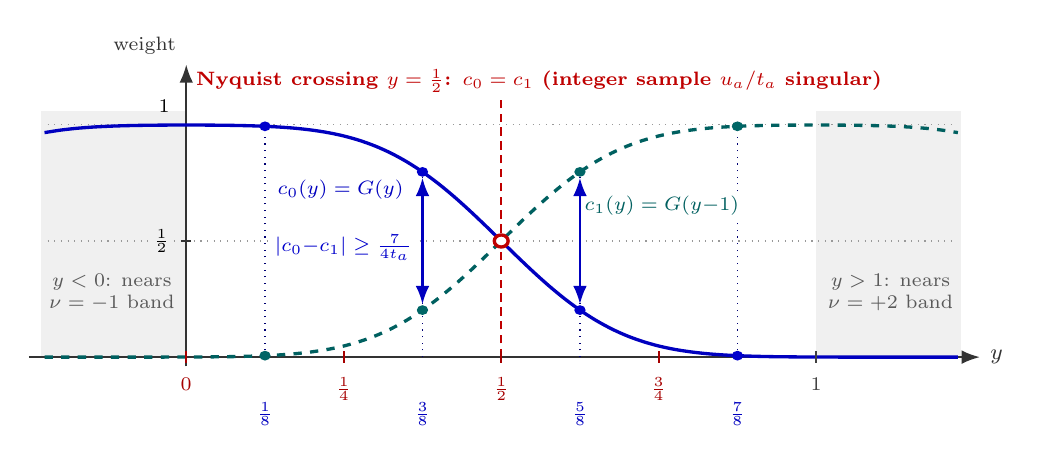
\begin{tikzpicture}[xscale=8.0, yscale=2.95, font=\footnotesize, >=Latex]
  % Shaded regions outside [0,1] where samples approach omitted alias passbands
  \fill[black!6] (-0.23, 0) rectangle (0, 1.06);
  \fill[black!6] (1.0, 0) rectangle (1.23, 1.06);
  \node[font=\scriptsize, text=black!65, align=center] at (-0.118, 0.28) {$y<0$: nears\\$\nu=-1$ band};
  \node[font=\scriptsize, text=black!65, align=center] at (1.118, 0.28) {$y>1$: nears\\$\nu=+2$ band};

  % Axes
  \draw[->, thick, black!80] (-0.25, 0) -- (1.26, 0) node[right] {$y$};
  \draw[->, thick, black!80] (0, -0.04) -- (0, 1.26) node[above left, font=\scriptsize] {weight};
  \draw[dotted, black!40] (-0.22, 1.0) -- (1.22, 1.0);
  \draw[dotted, black!40] (-0.22, 0.5) -- (1.22, 0.5);
  \draw[black!80, thick] (-0.008, 1.0) -- (0.008, 1.0);
  \draw[black!80, thick] (-0.008, 0.5) -- (0.008, 0.5);

  % Exact curves c_0(y) = G(y) and c_1(y) = G(y-1) at \tw = 8 (\alpha\sqrt\pi = 2\sqrt{8\ln 2})
  \draw[very thick, blue!75!black] plot[smooth] coordinates {
    (-0.225,0.9665) (-0.200,0.9771) (-0.175,0.9848) (-0.150,0.9901) (-0.125,0.9937)
    (-0.100,0.9961) (-0.075,0.9976) (-0.050,0.9985) (-0.025,0.9990) (0.000,0.9991)
    (0.025,0.9990) (0.050,0.9985) (0.075,0.9976) (0.100,0.9961) (0.125,0.9937)
    (0.150,0.9901) (0.175,0.9848) (0.200,0.9771) (0.225,0.9665) (0.250,0.9521)
    (0.275,0.9330) (0.300,0.9086) (0.325,0.8781) (0.350,0.8411) (0.375,0.7975)
    (0.400,0.7473) (0.425,0.6913) (0.450,0.6304) (0.475,0.5661) (0.500,0.5000)
    (0.525,0.4339) (0.550,0.3696) (0.575,0.3087) (0.600,0.2527) (0.625,0.2025)
    (0.650,0.1589) (0.675,0.1219) (0.700,0.0914) (0.725,0.0670) (0.750,0.0479)
    (0.775,0.0335) (0.800,0.0229) (0.825,0.0152) (0.850,0.0099) (0.875,0.0063)
    (0.900,0.0039) (0.925,0.0023) (0.950,0.0014) (0.975,0.0008) (1.000,0.0004)
    (1.025,0.0002) (1.050,0.0001) (1.075,0.0001) (1.100,0.0000) (1.150,0.0000)
    (1.200,0.0000) (1.225,0.0000)
  };
  \draw[very thick, teal!75!black, dashed] plot[smooth] coordinates {
    (-0.225,0.0000) (-0.200,0.0000) (-0.150,0.0000) (-0.100,0.0000) (-0.075,0.0001)
    (-0.050,0.0001) (-0.025,0.0002) (0.000,0.0004) (0.025,0.0008) (0.050,0.0014)
    (0.075,0.0023) (0.100,0.0039) (0.125,0.0063) (0.150,0.0099) (0.175,0.0152)
    (0.200,0.0229) (0.225,0.0335) (0.250,0.0479) (0.275,0.0670) (0.300,0.0914)
    (0.325,0.1219) (0.350,0.1589) (0.375,0.2025) (0.400,0.2527) (0.425,0.3087)
    (0.450,0.3696) (0.475,0.4339) (0.500,0.5000) (0.525,0.5661) (0.550,0.6304)
    (0.575,0.6913) (0.600,0.7473) (0.625,0.7975) (0.650,0.8411) (0.675,0.8781)
    (0.700,0.9086) (0.725,0.9330) (0.750,0.9521) (0.775,0.9665) (0.800,0.9771)
    (0.825,0.9848) (0.850,0.9901) (0.875,0.9937) (0.900,0.9961) (0.925,0.9976)
    (0.950,0.9985) (0.975,0.9990) (1.000,0.9991) (1.025,0.9990) (1.050,0.9985)
    (1.075,0.9976) (1.100,0.9961) (1.125,0.9937) (1.150,0.9901) (1.175,0.9848)
    (1.200,0.9771) (1.225,0.9665)
  };

  % Nyquist crossing at y = 1/2 (integer bin u_a/4 for u_a=2)
  \draw[red!75!black, thick, densely dashed] (0.5, 0) -- (0.5, 1.12);
  \draw[red!75!black, very thick, fill=white] (0.5, 0.500) circle [x radius=0.011, y radius=0.026];
  \node[red!75!black, fill=white, inner sep=1pt, font=\scriptsize\bfseries, align=center] at (0.56, 1.19)
    {Nyquist crossing $y=\tfrac12$: $c_0=c_1$ (integer sample $u_a/t_a$ singular)};

  % y-axis labels placed AFTER banner, cleanly clear of curves and dotted lines
  \node[above left=1pt and 2.5pt, font=\scriptsize] at (0, 1.0) {$1$};
  \node[left=3pt, fill=black!6, inner sep=1pt, font=\scriptsize] at (-0.008, 0.5) {$\tfrac12$};

  % Four integer-bin ticks u_a/4 \in {0, 1/4, 1/2, 3/4} in red, plus black reference tick at y=1
  \foreach \ux/\ulab in {0/0, 0.25/\tfrac14, 0.5/\tfrac12, 0.75/\tfrac34} {
    \draw[red!65!black, thick] (\ux, -0.025) -- (\ux, 0.025);
    \node[below=3pt, font=\scriptsize, text=red!65!black] at (\ux, -0.01) {$\ulab$};
  }
  \draw[black!75, thick] (1.0, -0.025) -- (1.0, 0.025);
  \node[below=3pt, font=\scriptsize, text=black!75] at (1.0, -0.01) {$1$};

  % Half-bin samples y = (u_a + 1/2)/4 for t_a = 4, \tw = 8: 1/8, 3/8, 5/8, 7/8
  \foreach \hx/\czero/\cone/\ymax/\hlab in {
    0.125/0.9937/0.0063/0.9937/\tfrac18,
    0.375/0.7975/0.2025/0.7975/\tfrac38,
    0.625/0.2025/0.7975/0.7975/\tfrac58,
    0.875/0.0063/0.9937/0.9937/\tfrac78} {
    \draw[blue!45!black, dotted] (\hx, 0) -- (\hx, \ymax);
    \fill[blue!80!black] (\hx, \czero) circle [x radius=0.009, y radius=0.021];
    \fill[teal!80!black] (\hx, \cone) circle [x radius=0.009, y radius=0.021];
    \node[below=13pt, font=\scriptsize\bfseries, text=blue!75!black] at (\hx, 0) {$\hlab$};
  }

  % Curve labels placed AFTER dotted lines, strictly inside (0.125, 0.375) and (0.625, 0.875)
  \node[blue!75!black, fill=white, inner sep=1.2pt, font=\scriptsize\bfseries] at (0.245, 0.72) {$c_0(y)=G(y)$};
  \node[teal!75!black, fill=white, inner sep=1.2pt, font=\scriptsize\bfseries] at (0.755, 0.65) {$c_1(y)=G(y{-}1)$};

  % Separation arrows at y = 3/8 and y = 5/8 (|c_0 - c_1| = 0.5949 > 7/16 = 0.4375)
  \draw[<->, thick, blue!75!black] (0.375, 0.228) -- (0.375, 0.772);
  \draw[<->, thick, blue!75!black] (0.625, 0.228) -- (0.625, 0.772);
  \node[fill=white, inner sep=1.2pt, font=\scriptsize, text=blue!80!black] at (0.250, 0.47)
    {$|c_0{-}c_1|\ge\tfrac{7}{4t_a}$};
\end{tikzpicture}
\caption{Retained alias weights $c_0(y)=G(y)$ and $c_1(y)=G(y-1)$ plotted at $\tw=8$ for $t_a=4$. Integer-bin samples $u_a/t_a\in\{0,\tfrac14,\tfrac12,\tfrac34\}$ (red ticks) include the Nyquist crossing $y=\frac12$ (at $u_a=t_a/2$), where $c_0=c_1$, making the two-alias operator singular. Negative half-bin samples $y=(u_a+\frac12)/t_a\in\{\tfrac18,\tfrac38,\tfrac58,\tfrac78\}$ (solid dots) stay strictly inside $(0,1)$ and at distance $\ge\frac{1}{2t_a}$ from $\frac12$, giving $|c_0-c_1|\ge\frac{7}{4t_a}$ and uniform conditioning $\|B_a^{-1}\|_\infty\le \frac47 t_a$.}
\label{fig:kernel-sampling}
\end{figure}

\paragraph{Triangular non-commuting factorization in $d$ dimensions.}
For general $R=t_1\cdots t_d=2^k$, put $A_a=\prod_{i<a}t_i$, write time indices as $j=\sum_{i=1}^d j_i A_i$ ($j_1$ least significant) and frequencies in reversed digit order $f(\mathbf u)=\sum_{i=1}^d u_i R/A_{i+1}$ ($u_d$ least significant). On axis $a\ge 2$, the fractional shift $\delta_a(\mathbf j)=(\sum_{i<a}j_i A_i)/A_a\in[0,1)$ depends on the \emph{original} digits below~$a$. We therefore spread the axes in \emph{descending} order $a=d,d-1,\dots,2$, forming $U=\mathcal S_2\mathcal S_3\cdots\mathcal S_d x$, so that whenever $\mathcal S_a$ acts, coordinates $1,\dots,a-1$ are still untouched. Dual to this in frequency space, shifting $f$ by $-\nu R/A_a$ modifies only the more significant frequency digits $u_1,\dots,u_{a-1}$ while leaving $u_a,\dots,u_d$ fixed. Consequently, Poisson summation along all $d-1$ spread axes factors into an exact \emph{triangular} operator product (Lemma~\ref{lem:bridge-A}):
\begin{equation}\label{eq:overview-triangular}
  F_{\mathbf t}U = \cA_2\cA_3\cdots\cA_d(F_R x), \qquad
  (\cA_a Z)_f = \sum_{\nu\in\Z} G\Bigl(\frac{u_a(f)+1/2}{t_a}-\nu\Bigr)\,Z_{(f-\nu R/A_a)\bmod R}.
\end{equation}
The operators $\cA_a$ do not commute, so deconvolution applies the two-alias cyclic inverses $B_2^{-1},B_3^{-1},\dots,B_d^{-1}$ in ascending order. Because $\|(B_2\cdots B_d)^{-1}\|_\infty\le (4/7)^{d-1}(R/t_1)\le R/t_1$, working precision $P=\Theta(p+\log R)$ and grid precision $q=P+2$ control both alias and fixed-point errors to $O(2^{-p}\max(1,\|x\|_\infty))$ (Theorem~\ref{thm:bridge-precision}). Finally, exposing each axis~$a$ by a single direct field interchange with the innermost axis~$d$ rather than a chain of adjacent swaps reduces the exposure overhead from $O(d^2)$ to $O(d)$ interchanges of cost $O\bigl(V d(1+\ell^\tau)\bigr)$ (Lemma~\ref{lem:bridge-D}).

\subsection{Butterfly layers as exact positional permutations}\label{sec:overview-walsh}

The central new idea of our middle transform is that the simultaneous butterfly layer of Proposition~\ref{prop:prop14-param} can itself execute \emph{any} permutation of the bit positions of a binary record address, bit-exactly and at the cost of $O(1)$ butterfly layers per slice.

\paragraph{Selective Walsh layers via three-layer cancellation.}
Consider an array of $2^{m_0}$ disk-valued records on the $q$-grid ($m_0=\log_2(R/r)=O(q)$), arranged so that a \emph{slice} selects one bit position from each of $D\le d$ consecutive $K$-bit address chunks. One black-box call to Proposition~\ref{prop:prop14-param} applies $H_0=\frac12\bigl(\begin{smallmatrix}1&1\\1&-1\end{smallmatrix}\bigr)$ to \emph{all} $D$ slice positions simultaneously ($H_{\mathrm{all}}$); we cannot disable individual chunks inside its recursive complex-network schedule. Observe, however, two $2\times 2$ identities involving the phase gate $S=\diag(1,i)$:
\begin{equation}\label{eq:overview-h3}
  H_0^3 = \tfrac12\,H_0, \qquad (H_0 S)^3 = \tfrac{1+i}{4}\,I.
\end{equation}
Indeed, $H_0^2=\frac12 I$ immediately gives $H_0^3=\frac12 H_0$, while cubing $H_0 S = \frac12\bigl(\begin{smallmatrix}1&i\\1&-i\end{smallmatrix}\bigr)$ yields $(H_0 S)^2 = \frac14\bigl(\begin{smallmatrix}1+i & 1+i\\ 1-i & i-1\end{smallmatrix}\bigr)$ and $(H_0 S)^3 = \frac{1+i}{4}I$. Suppose we want to apply $H_0$ only on an arbitrary subset $T$ of the $D$ slice positions ($s=|T|$) and act as the identity on the complement $U$ ($q_{\mathrm{sel}}=D-s$). Before each of \emph{three} full layer calls $H_{\mathrm{all}}$, we scan the array and multiply every record at address~$x$ by the scalar phase $(S_U z)(x) = i^{\sum_{j\in U} x_j} z(x)$. Because operators on distinct address bits tensor and commute, $(H_{\mathrm{all}} S_U)^3$ acts as $\frac12 H_0$ on every bit in~$T$ and collapses to $\frac{1+i}{4}I$ on every bit in~$U$. Rescaling by $2^s[2(1-i)]^{q_{\mathrm{sel}}}$ recovers the selective operator $H_T$ exactly (Lemma~\ref{lem:walsh-select}; Figure~\ref{fig:walsh-gadget}(a)).

\paragraph{Batched controlled flips without address movement.}
Next, conjugating $\diag(1,-1)$ by $H_0$ gives $2 H_0\diag(1,-1)H_0 = \bigl(\begin{smallmatrix}0&1\\1&0\end{smallmatrix}\bigr)$, whereas $2 H_0 I H_0 = I$. Consider $s$ pairwise disjoint control-target bit pairs $(c_j,t_j)$ whose targets $T=\{t_1,\dots,t_s\}$ lie in one slice, while the controls $c_j$ may lie \emph{anywhere} in the $m_0$-bit record address. Define the recordwise sign diagonal $(\CZ\,z)(x)=(-1)^{\sum_{j=1}^s x_{c_j} x_{t_j}}z(x)$. Then (Lemma~\ref{lem:cnot}; Figure~\ref{fig:walsh-gadget}(b))
\begin{equation}\label{eq:overview-cnot}
  \CNOT^{\otimes s} = 2^s H_T\,\CZ\,H_T
\end{equation}
moves every record from address~$x$ to the address with $x_{t_j}\mapsto x_{t_j}\oplus x_{c_j}$ for all $j=1,\dots,s$, using six full butterfly-layer calls and linear scans (Proposition~\ref{prop:cnot-batch}). Crucially, $\CZ$ never routes data between $c_j$ and $t_j$: it computes the parity $\sum_j x_{c_j} x_{t_j}\bmod 2$ from each record's address in $q^{O(1)}$ steps (absorbed by the record payload of $\Theta(rq)$ bits, Lemma~\ref{lem:transfer-long-record}) and negates the record in place.

\begin{figure}[t]
\setlength{\abovecaptionskip}{5pt}
\centering
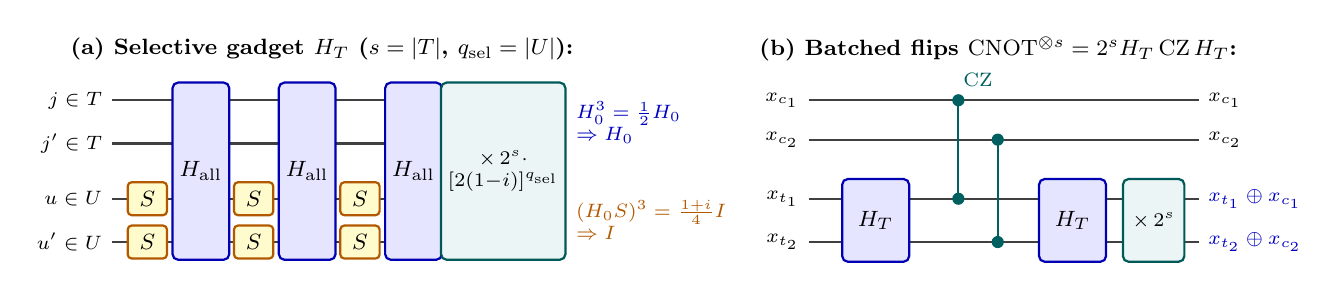
\begin{tikzpicture}[
  font=\footnotesize,
  >=Latex,
  gate/.style={draw=orange!70!black, fill=orange!15!yellow!20, thick, rounded corners=1.5pt, minimum width=0.50cm, minimum height=0.42cm, inner sep=1.5pt, align=center},
  layer/.style={draw=blue!70!black, fill=blue!10!white, thick, rounded corners=2pt, minimum width=0.72cm, inner sep=2pt, align=center},
  diagbox/.style={draw=teal!70!black, fill=teal!8!white, thick, rounded corners=2pt, inner sep=2.5pt, align=center},
  wire/.style={thick, black!75}
]
  % Panel (a): Selective Walsh gadget H_T
  \node[anchor=west, font=\footnotesize\bfseries] at (0, 2.55)
    {(a) Selective gadget $H_T$ ($s=|T|$, $q_{\mathrm{sel}}=|U|$):};

  % 4 wires: top 2 in T, bottom 2 in U
  \foreach \y/\wlab in {1.90/{$j\in T$}, 1.35/{$j'\in T$}, 0.65/{$u\in U$}, 0.10/{$u'\in U$}} {
    \draw[wire] (0.65, \y) -- (6.35, \y);
    \node[left, font=\scriptsize] at (0.65, \y) {\wlab};
  }

  % S gates on U wires before each of the 3 H_all layers
  \foreach \x in {1.10, 2.45, 3.80} {
    \node[gate] at (\x, 0.65) {$S$};
    \node[gate] at (\x, 0.10) {$S$};
  }
  % 3 full H_all boxes spanning all 4 wires
  \foreach \x in {1.78, 3.13, 4.48} {
    \node[layer, minimum height=2.25cm] at (\x, 1.00) {$H_{\mathrm{all}}$};
  }
  % Scalar box at end (wide enough so [2(1-i)]^{q_sel} fits cleanly)
  \node[diagbox, minimum height=2.25cm, minimum width=1.42cm, font=\scriptsize] at (5.62, 1.00)
    {$\times\,2^s\cdot$\\$[2(1{-}i)]^{q_{\mathrm{sel}}}$};

  \node[right, font=\scriptsize, align=left, text=blue!75!black] at (6.42, 1.62) {$H_0^3=\tfrac12 H_0$\\$\Rightarrow H_0$};
  \node[right, font=\scriptsize, align=left, text=orange!70!black] at (6.42, 0.38) {$(H_0 S)^3=\tfrac{1+i}{4}I$\\$\Rightarrow I$};

  % Panel (b): Batched CNOT = 2^s H_T CZ H_T
  \node[anchor=west, font=\footnotesize\bfseries] at (8.75, 2.55)
    {(b) Batched flips $\CNOT^{\otimes s}=2^s H_T\,\CZ\,H_T$:};

  % Control wires (top 2) and target wires in slice T (bottom 2)
  \draw[wire] (9.50, 1.90) -- (14.45, 1.90);
  \draw[wire] (9.50, 1.40) -- (14.45, 1.40);
  \draw[wire] (9.50, 0.65) -- (14.45, 0.65);
  \draw[wire] (9.50, 0.10) -- (14.45, 0.10);

  \node[left, font=\scriptsize] at (9.50, 1.90) {$x_{c_1}$};
  \node[left, font=\scriptsize] at (9.50, 1.40) {$x_{c_2}$};
  \node[left, font=\scriptsize] at (9.50, 0.65) {$x_{t_1}$};
  \node[left, font=\scriptsize] at (9.50, 0.10) {$x_{t_2}$};

  % First H_T on targets
  \node[layer, minimum height=1.05cm, minimum width=0.85cm] at (10.35, 0.375) {$H_T$};

  % CZ connections
  \draw[thick, teal!75!black] (11.40, 1.90) -- (11.40, 0.65);
  \fill[teal!75!black] (11.40, 1.90) circle (2.2pt);
  \fill[teal!75!black] (11.40, 0.65) circle (2.2pt);

  \draw[thick, teal!75!black] (11.90, 1.40) -- (11.90, 0.10);
  \fill[teal!75!black] (11.90, 1.40) circle (2.2pt);
  \fill[teal!75!black] (11.90, 0.10) circle (2.2pt);
  \node[above, font=\scriptsize, text=teal!75!black] at (11.65, 1.95) {$\CZ$};

  % Second H_T on targets + 2^s scaling
  \node[layer, minimum height=1.05cm, minimum width=0.85cm] at (12.85, 0.375) {$H_T$};
  \node[diagbox, minimum height=1.05cm, minimum width=0.78cm, font=\scriptsize] at (13.88, 0.375) {$\times\,2^s$};

  \node[right, font=\scriptsize] at (14.45, 1.90) {$x_{c_1}$};
  \node[right, font=\scriptsize] at (14.45, 1.40) {$x_{c_2}$};
  \node[right, font=\scriptsize, text=blue!75!black] at (14.45, 0.65) {$x_{t_1}\oplus x_{c_1}$};
  \node[right, font=\scriptsize, text=blue!75!black] at (14.45, 0.10) {$x_{t_2}\oplus x_{c_2}$};
\end{tikzpicture}
\caption{Turning simultaneous butterfly layers into exact controlled flips. (a)~Inserting $S=\diag(1,i)$ on $U$ before three full layers cancels $U$ to $\frac{1+i}{4}I$ while leaving $\frac12 H_0$ on $T$. (b)~Sandwiching the recordwise sign diagonal $\CZ$ between two selective $H_T$ gadgets flips all target address bits $t_j\in T$ by distant controls $c_j$ in six layer calls.}
\label{fig:walsh-gadget}
\end{figure}

\paragraph{Every positional permutation is $O(1)$ CNOT stages, and is bit-exact.}
Every permutation~$\pi$ of the $m_0$ record-address bit positions factors on its cycles as $\pi = I_1\circ I_0$, a product of two involutions, and each involution is a set of disjoint two-bit swaps implemented by three stages of disjoint CNOTs (Lemma~\ref{lem:walsh-involutions}). We partition the $m_0$ positions into $N_{\mathrm{slice}}\le m_0/d + K$ slices of $D\le d$ chunks, plus fewer than~$K$ leftover positions handled by linear two-digit stream swaps. Grouping each of the six CNOT stages by target slice then executes any positional permutation~$\pi$ in at most $36 N_{\mathrm{slice}}$ layer calls, costing $O\bigl(V[(m_0/d+K)d^{\lambda'}+K]\bigr)=O(V\ell d^{\lambda'})$ steps, the same order as the FFT butterfly rounds themselves (Theorem~\ref{thm:positional-perm}).

Why does fixed-point truncation introduce zero error across complex linear combinations? Before each CNOT batch on a $q$-grid disk array, we append $8d$ zero fractional bits to lift to precision $q_*=q+8d$ (Lemma~\ref{lem:walsh-lift}). Each normalized $D$-bit layer divides by $2^D$ ($D\le d$), while $S_U$ and $\CZ$ multiply by units in $\{\pm 1,\pm i\}$, so throughout both $H_T$ gadgets every intermediate entry lies on a dyadic grid of denominator exponent at most $q+s+3D\le q+4d < q_*$. Because Proposition~\ref{prop:prop14-param} evaluates each layer \emph{exactly} internally (using its guard~$\Delta$) before a single final truncation $Q_{q_*}$, every truncation discards only trailing zeros (Lemma~\ref{lem:walsh-exact}). Once $\CNOT^{\otimes s}$ completes, the array is an exact permutation of the original $q$-grid records, so stripping the $8d$ zero bits returns to the $q$-grid bit-exactly and resets denominator growth before the next batch.

\subsection{A direct tensor FFT and where \texorpdfstring{$2^{-46}$}{2\^{}\{-46\}} comes from}\label{sec:overview-fft}

\paragraph{Direct decimation-in-frequency tensor FFT.}
With exact positional permutations available at layer cost, Bluestein's chirp reduction and polynomial-ring convolutions over $\C[y]/(y^r+1)$ disappear completely. We evaluate $F_{\mathbf t}U$ on the $q$-grid ($t_d=r=2^\ell$, $t_i\in\{r/2,r\}$; Theorem~\ref{thm:direct-fft}) in four steps.
\begin{enumerate}[label=(\arabic*),nosep,leftmargin=*]
  \item Run a standard length-$r$ DIF FFT inside each contiguous record along axis~$d$.
  \item Apply the exact positional permutation~$L$ (Lemma~\ref{lem:walsh-layout}) to interleave $K$-bit chunks of the $d-1$ record axes.
  \item Execute the $\ell$ DIF bit-levels across all $d-1$ record axes in parallel: at most~$K$ prefix/leftover levels by exact individual butterflies in $O(VdK)$, and the remaining chunk levels by one call to Proposition~\ref{prop:prop14-param} per level in $O(V\ell d^{\lambda'})$. At each level~$v$, multiplying $d-1$ separately rounded twiddles would accumulate $O(d\ell\cdot 2^{-q})$ error. Instead, we combine all participating axis twiddles into a \emph{single} exact index $J(x)=\sum_i (r/2^{v+1})b_i j_i^{<v}\bmod r$, where $2^{v+1}$ is the DIF subproblem length, $b_i\in\{0,1\}$ is axis~$i$'s branch bit at level~$v$, and $j_i^{<v}$ is its lower $v$-bit index. Looking up that index in one $2r$-entry disk-valued phase table (Lemma~\ref{lem:phase-table}) incurs error $<6\cdot 2^{-q}$ per level regardless of~$d$.
  \item Apply the exact positional permutation $(LB)^{-1}=B^{-1}L^{-1}$ (Theorem~\ref{thm:positional-perm}) to undo both the chunk layout~$L$ and the DIF bit-reversal~$B$ in one pass.
\end{enumerate}
Because every exact DIF round is an $\ell^\infty$ contraction and the positional maps are exact, the $\ell$ last-axis levels and at most~$\ell$ record-axis rounds accumulate total error strictly below $12\ell\cdot 2^{-q}$ (Corollary~\ref{cor:walsh-middle}), with no $R/r$ error amplification and no output bit-widening.

\paragraph{Cost balance and the exponent $\kappa=2^{-46}$.}
Dividing the cost of one bridge call by $V=RP=\Theta(n)$ leaves the five normalized terms of Table~\ref{tab:cost-walsh}, where $P=\Theta(\log n)$, $d=\lfloor k^\eps\rfloor=\Theta(P^\eps)$, $\ell=\Theta(P^{1-\eps})$, $K=\lfloor d^c\rfloor=\Theta(P^{\eps c})$, and $\mathsf m(N)=\mathsf M(N)/N=(\log N)^{O(1)}$. Individual prefix butterfly rounds cost $O(dK)$ (gap $1-\eps(1+c)$ below $P^1$), simultaneous layers and the exact positional maps $L,(LB)^{-1}$ cost $O(\ell d^{\lambda'})$ (gap $\eps(1-\lambda')$), and the last-axis FFT and combined twiddle products cost $O(\ell\,\mathsf m(P))$ (gap $\eps$ up to $\log P$). Direct axis exposures and restorations cost $O\bigl(d(1+\ell^\tau)\bigr)$ (gap $(1-\eps)(1-\tau)$), and spreading and two-alias cyclic solves cost $O\bigl(d(\mathsf m(P)+\mathsf m(P^2))\bigr)$ (gap $1-\eps$ up to $\log P$). With the external chunk-swap term $P K^{\tau-1}$ gone, we are free to choose $c$ tiny so internal layer basis changes never bind. This leaves the butterfly-layer gap $g_{\mathrm{lay}}=\eps(1-\lambda') < (1-\sigma)/C_1$ as the sole bottleneck, now \emph{linear} in the complex network's deficit $1-\sigma$.

At $h=100$ ($m=10^6$), the complex network of~\cite{OAI26} has exact relative deficit $\eta_c=(W_c m - s_c)/(W_c m)=73/19{,}906{,}842{,}167{,}500$. Using the elementary rational bound $\ln 10^6 < 14$ (via $e^7>\sum_{j=0}^{11}7^j/j!>1000$, sharpening $\ln m<20$ in~\cite{OAI26}), Proposition~\ref{prop:deficits} certifies $s_c/W_c < m^\sigma$ at $\sigma=1-\xi$ with $\xi=2^{-42}$ (since $73\cdot 2^{42} > 14\cdot 19{,}906{,}842{,}167{,}500$) and $\tau=1-4\xi=1-2^{-40}$ for the bit network. Moreover, the guard bound $B_{\mathrm{net}}<10^{66}=m^{11}$ admits guard exponent $C_1=11+3=14$ (Proposition~\ref{prop:prop14-param}; cf.~\cite[\S5.4]{OAI26}). Setting $\eps=1/15$, $\beta=1/64$, $c=\xi/256$, $\lambda=1-\frac{63}{64}\xi$, and $\lambda'=1-\frac{31}{32}\xi$ gives $g_{\mathrm{lay}}=\eps(1-\lambda')=\frac{31}{480}\xi > \frac{1}{16}\xi = 2^{-46}$, yielding $\kappa=2^{-46}$ with positive slack (Section~\ref{sec:main-rows}). In short, Bluestein's chunk layout is capped quadratically at $(1-\tau)^2/(C_1\tau)\approx 2^{-83.8}$, whereas Walsh-layer permutations reach $(1-\sigma)/C_1\approx 2^{-45.8}$ linearly and already achieve $\kappa=2^{-56}$ under the printed constants of~\cite[Prop.~14]{OAI26}.

\subsection{Formal verification}\label{sec:overview-lean}

Section~\ref{sec:lean} describes our Lean~4 formalization~\cite{Lean26} of Theorem~\ref{thm:lean}. It constructs a single finite-alphabet multi-stack Turing machine in Mathlib's \texttt{Turing.TM2ComputableInTime} model and proves \texttt{SubNLogN.Challenge.IntMulSubNLogN} (exact multiplication of all $(a,b)\in\N^2$ within $C\,L\,(\log_2 L)^{1-2^{-46}}$ steps for input length $L\ge N_0$) from Lean's three standard axioms alone. That development verifies both $h=100$ finite networks, their rank and endpoint certificates, all stream and parameter-transfer procedures, and the analytical error bounds from scratch. The formal proposition does not express syntactic CRT-freeness and formalizes only the $\kappa=2^{-46}$ Walsh machine (deriving $2^{-47}$, $2^{-56}$, and $o(n\log n)$ by exponent monotonicity). It differs from the text primarily in two respects. First, it uses tie-upward nearest rounding (our bridge theorems are proved in Lean for arbitrary nearest rounding). Second, it instantiates the inner $O(N\log N)$ multiplier and its root offset via our independent Lean~4 formalization (\texttt{IntMulTM.\allowbreak intMul\_\allowbreak TM2\_\allowbreak nlogn}, kernel-checked within~\cite{Lean26}) of the two-dimensional multiplier of~\cite{MS}, which distributes its own separate Lean development.

\setlength{\textfloatsep}{20.0pt plus 2.0pt minus 4.0pt}
\setlength{\intextsep}{12.0pt plus 2.0pt minus 2.0pt}
\section{Preliminaries}\label{sec:prelim}

This section sets up the shared definitions and external facts needed to state and prove the bridge, permutation, and Fourier-transform bounds of Sections~\ref{sec:bridge}--\ref{sec:main}. Section~\ref{sec:notation} collects global notation in Table~\ref{tab:notation}, and Section~\ref{sec:prelim-model} specifies the multitape Turing machine model, tape array layout, and fixed-point rounding rules. Section~\ref{sec:prelim-dft} fixes our normalized discrete Fourier transform conventions and the two-call real convolution identity, while Section~\ref{sec:prelim-oai} records the two black-box facts borrowed from~\cite{OAI26}. A first-time reader may skim Table~\ref{tab:notation} and Section~\ref{sec:prelim-oai} and return to them when cited.

\subsection{Notation}\label{sec:notation}

We begin by fixing basic conventions for logarithms, index ranges, and $\ell^\infty$ norms used across all sections. Logarithms are natural, written $\ln$, unless written $\log_2$. Following~\cite{OAI26}, we write $\lg n=\max\{\lceil\log_2 n\rceil,1\}$, so $\lg R=\log_2 R$ whenever $R\ge 2$ is a power of two. For a positive integer $N$ we write $[N]=\{0,\dots,N-1\}$. For a complex vector~$x$, $\|x\|_\infty=\max_j|x_j|$ denotes the largest complex modulus, and for a linear map~$A$, $\|A\|_\infty$ is the induced $\ell^\infty$ operator norm, equal to the maximum absolute row sum. For an array of polynomial records in $\Rr_r=\C[y]/(y^r+1)$, $\|\cdot\|_\infty$ denotes the largest modulus of any complex coefficient across the array. Table~\ref{tab:notation} summarizes global symbols.

\begin{table}[!t]
\centering
\small
\renewcommand{\arraystretch}{0.92}
\caption{Reference summary of global symbols and parameters used throughout the paper. Bridge-specific quantities are defined in Section~\ref{sec:bridge}, and finite-network parameters in Section~\ref{sec:prelim-oai}.}
\label{tab:notation}
\begin{tabular}{@{}>{\raggedright}p{0.27\textwidth}>{\raggedright\arraybackslash}p{0.67\textwidth}@{}}
\toprule
Symbol & Meaning\\
\midrule
$n,\ \kappa$ & bit length of each input integer; log-saving exponent in $O(n(\lg n)^{1-\kappa})$\\
$R=t_1\cdots t_d,\ k=\lg R$ & bridge transform length ($t_i\ge 2$ powers of two, $d$ dimension, $r=t_d=2^\ell$) and its binary logarithm\\
$M=R/r,\ \mathsf M(N),\ \mathsf m(N)$ & number of records; cost of the independent $N$-bit integer multiplier; $\mathsf m(N)=\mathsf M(N)/N$\\
$p,\ P$ & target precision of a bridge call (errors in units of $2^{-p}$); internal working precision of the bridge\\
$q,\ v=2^{-q}$ & dyadic grid precision of Sections~\ref{sec:walsh}--\ref{sec:direct-fft}, instantiated by the bridge at $q=P+2$; unit of that grid\\
$w$ & two's-complement component width; $w=q+2=P+4$ in the bridge schedule~\eqref{eq:schedule}\\
$\tw,\ \alpha$ & alias width parameter and Gaussian width parameter of the bridge kernel\\
$a\in\{2,\dots,d\},\ \nu\in\Z$ & spread-axis index of the bridge; alias index in Poisson summation\\
$g_a,\ G$ & negative half-bin carrier on axis $a$; Fourier transform of $\sinc(s)\,e^{-\pi s^2/\alpha^2}$\\
$f(\mathbf u),\ A_a$ & scalar frequency index with digits $u_1,\dots,u_d$; $A_a=\prod_{i<a}t_i$, the cycle length of $B_a$\\
$c_0,\ c_1,\ c_{\max}$ & retained alias weights $G((u+\tfrac12)/t)$ and $G((u+\tfrac12)/t-1)$; $\max(c_0,c_1)$\\
$\cA_a,\ B_a$ & full alias operator on axis $a$; two-term cyclic operator (its two-alias truncation)\\
$\Rr_r=\C[y]/(y^r+1)$ & record ring specifying the $r$-coefficient record layout\\
$\Cg_q,\ \mathbb{D}_q$ & fixed-point grid $2^{-q}(\Z+i\Z)$; disk grid $\{z\in\Cg_q:|z|\le 1\}$\\
$Q_q,\ \Quant_q$ & componentwise truncation toward zero to $\Cg_q$; componentwise nearest rounding to $\Cg_q$\\
$V$ & logical bit volume of a stored array\\
$K=\lfloor d^c\rfloor,\ D$ & chunk width and number of active $K$-bit chunks ($1\le D\le d$) in a simultaneous butterfly layer\\
$A,\ q_{\mathrm{rad}},\ \Gamma$ & layer and stream interface symbols: prefix range (written $P$ in~\cite[Prop.~14]{OAI26}), fixed radix (written $q$ in~\cite{OAI26}), and self-delimiting header code~\cite[(1)]{OAI26}\\
$H_0,\ S$ & normalized butterfly $(u,v)\mapsto((u+v)/2,(u-v)/2)$ and phase gate $\diag(1,i)$\\
$h=100,\ m=h^3=10^6$ & ground-set size parameters of the fixed triple networks of~\cite{OAI26}\\
$W_b,s_b;\ W_c,s_c$ & role counts and recursive call counts of the bit and complex networks ($s_b<W_bm$, $s_c<W_cm$)\\
$\eta_b,\ \eta_c;\ \tau,\ \sigma$ & relative rank deficits $(Wm-s)/(Wm)$ and network exponents ($s_b/W_b<m^\tau$, $s_c/W_c<m^\sigma$)\\
$\beta,\ \nu_{\mathrm{net}},\ C_1$ & leaf-stopping exponent, guard degree $\min\{j\ge 1:m^j\ge B_{\mathrm{net}}\}=11$, and guard exponent of the layer\\
$\eps,\ c,\ \lambda,\ \lambda'$ & schedule and recurrence exponents; $d=\lfloor k^\eps\rfloor$, $K=\lfloor d^c\rfloor$\\
$S,\ L,\ B,\ K$ & also reused locally (defined at use): suffix range or pre-scale/series width~$S$, layout map or cycle/input length~$L$, bit-reversal or suffix range~$B$, general chunk width~$K$ (and $K_0,K_*$)\\
\bottomrule
\end{tabular}
\end{table}

\subsection{Machine model and fixed-point arithmetic}\label{sec:prelim-model}\label{sec:prelim-grids}

This subsection defines the multitape Turing machine cost model, the sequential tape representation of multidimensional arrays, and the fixed-point complex grids on which the algorithm operates. Our complexity bounds refer to the standard deterministic multitape Turing machine model of~\cite{SS71,HvdH21,OAI26} with one fixed finite alphabet and a fixed finite number of one-dimensional tapes. In each step the machine reads and writes at most one cell per tape and moves each head by at most one cell. The running time is the total number of steps, so every scan, head movement, rewind, counter update, and workspace cleanup is charged. The input is $x\#y$ with $x,y\in\{0,1\}^n$, and the output is the $2n$-bit binary representation of their product~\cite[\S1]{OAI26}.

Following~\cite[\S2]{OAI26}, an array on $[a_1]\times\cdots\times[a_t]$ with $a_i\ge 1$ is stored in lexicographic order with the first coordinate most significant, so addresses are implicit in tape position rather than stored per entry. Adjacent spectator fields, meaning address fields that the current operation leaves untouched, may be collapsed into one field whose range is their product. An address permutation~$f$ moves the entry at address~$x$ to $f(x)$, giving $(fA)(f(x))=A(x)$. The \emph{logical bit volume}~$V$ of an array is its total number of stored data bits; temporary copies on work tapes are charged in running time without replacing~$V$ in recursive bounds. Integer parameters in procedure headers use the self-delimiting code $\Gamma(v)=0^{b_v-1}\mathrm{bin}_{b_v}(v)$ of length $2b_v-1$, where $b_v=\lfloor\log_2 v\rfloor+1$ for $v\ge 1$~\cite[(1)]{OAI26}.

\paragraph{Independent integer multiplier.}
Ordinary products of $N$-bit integers are delegated to an independent deterministic multiplier of worst-case cost $\mathsf M(N)=N\,\mathsf m(N)$, such as Sch\"onhage--Strassen multiplication~\cite{SS71} with $\mathsf m(N)=O(\lg N\lg\lg N)$. It runs as a black-box subroutine on dedicated work tapes that are clean on return, leaving the caller's other tapes untouched and making no recursive call to Algorithm~1.

\paragraph{Grids, rounding, and faithful tables.}
All stored complex numbers lie on dyadic fixed-point grids. The next definition fixes the grid $\Cg_P$ and disk grid $\mathbb{D}_P$ at an arbitrary integer precision $P\ge 0$, and specifies how records of $r$ complex numbers in $\mathbb{D}_q$ are stored in two's-complement binary at precision $q\ge 0$. It also introduces the two rounding operators, truncation toward zero $Q_P$ and nearest rounding $\Quant_P$, whose bounds~\eqref{eq:rounding} govern where each is used below.

\begin{definition}[Fixed-point grids and rounding]\label{def:grid}
For an integer precision $P\ge 0$, define the \emph{fixed-point grid} $\Cg_P=\{2^{-P}(a+ib):a,b\in\Z\}$ (also called
the \emph{$P$-grid}) and the \emph{disk grid} $\mathbb{D}_P=\{z\in\Cg_P:|z|\le 1\}$. At precision $q\ge 0$, a
\emph{disk-grid record} is an element $\sum_{j<r}z_j y^j\in\Rr_r=\C[y]/(y^r+1)$ with every $z_j\in\mathbb{D}_q$, stored
in coefficient order $j=0,\dots,r-1$; a \emph{disk array} is an array of records with $\|z\|_\infty\le 1$. Each real or
imaginary component is stored as $2^{-q}$ times a signed $w$-bit two's-complement integer, most significant bit first,
with the real component before the imaginary one~\cite[Prop.~14]{OAI26}; any width $w\ge q+2$ represents every
disk-grid component, including $\pm 1$. For $z\in\C$ and any integer $P\ge 0$:
\begin{itemize}[leftmargin=*]
  \item $Q_P(z)$ truncates the real and imaginary parts of $z$ toward zero to $2^{-P}\Z$~\cite[(26)]{OAI26};
  \item $\Quant_P(z)$ rounds the real and imaginary parts of $z$ to a nearest element of $2^{-P}\Z$ (for concreteness
    with ties to even, though every bound we prove holds for any nearest-rounding tie rule).
\end{itemize}
Both operators act coefficientwise on records and arrays.
\end{definition}

For every $z\in\C$ and integer $P\ge 0$,
\begin{equation}\label{eq:rounding}
  |Q_P(z)-z|<\sqrt2\cdot 2^{-P},\qquad |Q_P(z)|\le |z|,\qquad |\Quant_P(z)-z|\le\tfrac{\sqrt2}{2}\cdot 2^{-P}.
\end{equation}
In particular, $Q_q$ maps the closed unit disk into $\mathbb{D}_q$, so any exact disk-preserving operator followed by $Q_q$ keeps every stored coefficient inside $\mathbb{D}_q$, whereas nearest rounding can step outside the unit disk near $\pm 1$. By contrast, inside the bridge's spreading and deconvolution stages, where norms are tracked explicitly, $\Quant_q$ halves the per-step rounding error. Precomputed transcendental entries for filter taps, solver parameters, and unit phases are never assumed to be exact nearest roundings. Instead, they are \emph{faithful} approximations computed by truncated rational series with certified error at most $2^{-q}$ for real entries and $2\cdot 2^{-q}$ for complex taps and disk-valued unit phases.

\subsection{Discrete Fourier transforms}\label{sec:prelim-dft}\label{sec:prelim-oai-transform}

This subsection fixes the normalization and sign convention of our one-dimensional and multidimensional Fourier transforms and records the identity that recovers a real cyclic convolution from two forward transforms. Dividing by the transform length~$R$ in the definition below ensures that every exact transform is an $\ell^\infty$ contraction, keeping intermediate entries bounded without rescaling across dimensions.

\begin{definition}[Normalized transforms]\label{def:dft}
For an integer $R\ge 1$, the normalized positive one-dimensional DFT $F_R\colon\C^R\to\C^R$ is
$(F_R x)_u=\frac1R\sum_{j\in[R]}x_j e^{2\pi iju/R}$. For $\mathbf t=(t_1,\dots,t_d)$ with $R=t_1\cdots t_d$, the
normalized positive tensor DFT $F_{\mathbf t}=F^+_{\mathbf t}=F_{t_1,\dots,t_d}$ acts on arrays indexed by
$[t_1]\times\cdots\times[t_d]$ via
\[
  (F_{\mathbf t}U)_{u_1,\dots,u_d}=\frac1R\sum_{j_1,\dots,j_d}U_{j_1,\dots,j_d}\,
  \exp\Bigl(2\pi i\sum_{i=1}^d\frac{j_i u_i}{t_i}\Bigr).
\]
\end{definition}

By the triangle inequality, $\|F_R\|_\infty\le 1$ and $\|F_{\mathbf t}\|_\infty\le 1$. The cyclic convolution $(a\circledast b)_j=\sum_{l\in[R]}a_l b_{(j-l)\bmod R}$ satisfies $F_R(a\circledast b)=R\,(F_R a)\odot(F_R b)$, where $\odot$ denotes entrywise multiplication. For real vectors $a,b\in\R^R$ and $z=a+ib$, the \emph{two-call identity} (cf.~\cite{MS}) recovers $a\circledast b$ from two forward transforms of length~$R$:
\begin{equation}\label{eq:two-call}
  a\circledast b=-\frac{R^2}{2}\,\mathrm{Im}\Bigl(F_R\bigl(\overline{(F_R z)\odot(F_R z)}\bigr)\Bigr).
\end{equation}
Indeed, $\sum_{u\in[R]}e^{2\pi i(j-k)u/R}$ equals $R$ for $j=k$ and $0$ otherwise, so $F_R(\overline{F_R w})=R^{-1}\overline w$ for every $w\in\C^R$. Applying this relation to $w=z\circledast z=(a\circledast a-b\circledast b)+2i(a\circledast b)$, for which $(F_R z)\odot(F_R z)=R^{-1}F_R w$, gives $F_R(\overline{(F_R z)\odot(F_R z)})=R^{-2}\overline w$, whose imaginary part is $-2R^{-2}(a\circledast b)$.

For completeness, and only for the Bluestein comparison in Appendix~\ref{app:bluestein}, we also record the synthetic transforms of~\cite[\S6]{OAI26}; a first-time reader may skip this paragraph. Over the negacyclic ring $\Rr_r=\C[y]/(y^r+1)$ with $r=2^\ell\ge 2$, multiplication by~$y$ is an $\ell^\infty$ isometry. For any power of two $t\mid 2r$, setting $\omega_t=y^{2r/t}\in\Rr_r$ defines contractions $F_t^\mp\colon\Rr_r^t\to\Rr_r^t$ by $(F_t^\mp z)_j=t^{-1}\sum_{k<t}\omega_t^{\mp jk}z_k$ satisfying $F_t^+ F_t^-=t^{-1}I$. With $B_t$ denoting $(\lg t)$-bit binary reversal on $[t]$, in-place decimation in frequency and its reverse compute $B_t F_t^-$ and $F_t^+ B_t^{-1}$. For $\mathbf t'=(t_1,\dots,t_{d-1})$ with $t_i\mid 2r$, we write $F_{\mathbf t'}^\pm=\bigotimes_{i=1}^{d-1}F_{t_i}^\pm$ and $B=\bigotimes_{i=1}^{d-1}B_{t_i}$. Our direct complex tensor FFT in Section~\ref{sec:direct-fft} uses no ring products or synthetic transforms in $\Rr_r$, keeping $\Rr_r$ only to specify the contiguous $r$-coefficient record format.

\paragraph{Motivation from two-dimensional fractional shifts.}
In dimension two ($R=t_1 r$), Section~\ref{sec:overview-bridge} read the Cooley--Tukey twiddle factor as a fractional shift of row~$j_1$ by $j_1/t_1$~\cite{MS} and spread each row by a sinc-Gaussian filter. Applying Poisson summation then relates $F_{t_1,r}$ of the spread array, on the same $t_1\times r$ grid, to a cyclic alias mixture of $F_R x$ along each column in which two aliases dominate. With a real kernel the two retained alias weights coincide at the Nyquist column $u_2=r/2$; \cite{MS} handles this by a separate alternating-sum identity, and the coincidence prevents cycle-length-independent conditioning in higher dimensions. Section~\ref{sec:bridge} removes both obstacles for general $d\ge 2$ via a negative half-bin carrier and descending axis spreading.

\subsection{Ingredients from \texorpdfstring{\cite{OAI26}}{[OAI26]}}\label{sec:prelim-oai}

This subsection states the two results from~\cite{OAI26} that our written proofs use as black boxes, and summarizes the general-parameter tape procedures derived from them in Appendix~\ref{app:parameter-transfer}. Appendix~\ref{app:oai} restates the borrowed statements in full and records the symbol-renaming map from~\cite{OAI26}: its prefix range~$P$ becomes~$A$, its fixed radix~$q$ becomes $q_{\mathrm{rad}}$, and its box size~$T$ corresponds to~$R$.

First, Fact~\ref{fact:oai-streams} packages five linear-time sequential tape-stream primitives on arrays of bit volume~$V$. These primitives cover digit permutations, stream splits and merges, cyclic row distributions into $W$ role streams, prime-radix modular shifts, and exact fixed-width binary arithmetic.

\begin{fact}[Elementary tape operations~{\cite[Lemmas~3--4]{OAI26}}]\label{fact:oai-streams}
Fix an integer radix $q_{\mathrm{rad}}\ge 2$. On a stored array of logical bit volume $V$ on a fixed number of
finite-alphabet tapes, the following operations run in $O(V)$ steps (including counter initialization, head resets, and
clearing visited workspace):
\begin{enumerate}[label=(\arabic*),nosep,leftmargin=*]
  \item applying any fixed permutation to the pair of digit values at two specified radix-$q_{\mathrm{rad}}$ address
    positions, or moving one specified radix-$q_{\mathrm{rad}}$ digit position to another while preserving the order of
    intervening positions;
  \item splitting an array on a specified radix-$q_{\mathrm{rad}}$ digit, applying a fixed pointwise map to the aligned
    streams, and merging them back;
  \item within each prefix of an array on $[A]\times[R_{\mathrm{row}}]\times[B]$, distributing whole rows cyclically
    into a fixed number $W$ of role streams and, when $W\mid R_{\mathrm{row}}$, merging them in any fixed order of row
    classes;
  \item when $q_{\mathrm{rad}}$ is prime and a target field $y\in[q_{\mathrm{rad}}^b]$ follows control fields of
    $O(b)$ digits each across arbitrary spectators, shifting $y\mapsto y+a(\mathrm{controls})\pmod{q_{\mathrm{rad}}^b}$
    for any offset computable in $b^{O(1)}$ time (in particular any fixed rational linear combination with denominators
    coprime to $q_{\mathrm{rad}}$), or multiplying $y$ modulo $q_{\mathrm{rad}}^b$ by a fixed rational unit prime to
    $q_{\mathrm{rad}}$;
  \item exact fixed-width signed binary addition, subtraction, sign change, bit-order reversal within a component, and
    multiplication or division by a power of two when guard bits prevent overflow or inexact truncation.
\end{enumerate}
\end{fact}

Second, Fact~\ref{fact:oai-networks} states the finite algebraic certificates of the two fixed linear circuits at $h=100$ and $m=h^3=10^6$. The strict inequalities $s_b<W_b m$ and $s_c<W_c m$, which say that each network's recursive rank sum falls short of the trivial product of its role count and the dimension~$m$, are the sole source of the sub-$n\log n$ exponent saving.

\begin{fact}[Finite linear networks with a rank deficit~{\cite[Props.~7--8]{OAI26}}]\label{fact:oai-networks}
At ground-set parameter $h=100$ and dimension $m=h^3=10^6$, there exist two fixed finite linear circuits (over the
three-element subsets of $[h]$) with the following certified role counts, recursive rank sums, and endpoint actions for
arbitrary initial values on all auxiliary scratch roles:
\begin{enumerate}[label=(\alph*),nosep,leftmargin=*]
  \item \emph{Bit shear network}: a fixed pointwise XOR circuit on $W_b$ roles equipped with rational $m\times m$
    terminal and gate matrices whose completed scalar action is a role permutation $\rho_b$ satisfying
    $M_{\mathrm{out}(\rho_b(w))}-M_{\mathrm{in}(w)}=I_m$ for every input role $w$ (implementing the common address shear
    $(H,D)\mapsto(H+D,D)$ on $m$-tuples of address fields). Its role count $W_b$ and total edge-difference rank
    $s_b=\sum_e\operatorname{rank}_{\Q}(M_{\mathrm{head}(e)}-M_{\mathrm{tail}(e)})$ are
    \[
      W_b=177\,176\,569\,091\,445\,000\,000,\qquad
      s_b=177\,176\,569\,088\,785\,861\,287\,000\,000<W_b m,
    \]
    giving relative rank deficit $\eta_b=(W_b m-s_b)/(W_b m)=339/22\,587\,335\,000\,000$.
  \item \emph{Complex phase network}: a fixed scalar linear circuit on $W_c$ roles with coefficients in
    $\{0,\pm 1,\pm\tfrac12\}$ and nested binary subspace labels in $\mathbb F_2^m$ whose edge-residual orthonormal bases
    have total dimension $s_c$, implementing $C^{\otimes m}$ with $C=\frac{1+i}{2}I+\frac{1-i}{2}X$ on every role after
    prescribed source/sink diagonal phases and bank restoration, with
    \[
      W_c=1\,873\,807\,244\,643\,542\,670\,000,\qquad
      s_c=1\,873\,807\,244\,636\,671\,267\,308\,000\,000<W_c m,
    \]
    giving relative rank deficit $\eta_c=(W_c m-s_c)/(W_c m)=73/19\,906\,842\,167\,500$.
\end{enumerate}
\end{fact}

\paragraph{What the written proof depends on.}
No result of~\cite{HvdH21} is used anywhere in our proofs. Our written proof of Theorem~\ref{thm:main} imports only Facts~\ref{fact:oai-streams} and~\ref{fact:oai-networks}, corresponding to~\cite[Lemmas~3--4 and Props.~7--8]{OAI26}, as black boxes. Every other step is proved in Sections~\ref{sec:bridge}--\ref{sec:main} or re-derived in Appendix~\ref{app:parameter-transfer} by following~\cite[\S\S4--5]{OAI26} with all exponents and guard parameters exposed. Lemmas~15--21 and Proposition~18 of~\cite{OAI26}, covering synthetic ring transforms, chunk-swap layout, packed products, ring convolution, Gaussian resampling, and Bluestein's chirp, are unused on the main route and appear only for comparison in Appendix~\ref{app:bluestein}. The Lean~4 proof of Theorem~\ref{thm:lean} uses neither black box, constructing and verifying both $h=100$ networks, their algebraic certificates, and all Turing machine stream procedures from scratch.

\paragraph{Parameter-exposed tape procedures.}
As printed, \cite[Lemma~12 and Prop.~14]{OAI26} fix $\tau=\sigma=1-2^{-50}$, $\beta=\tfrac12$, and $C_1=20$. In Appendix~\ref{app:parameter-transfer} we follow~\cite[\S\S4--5]{OAI26} with all structural parameters exposed, deriving two procedures from Facts~\ref{fact:oai-streams} and~\ref{fact:oai-networks} together with Lemma~\ref{lem:transfer-long-record} for long-record address scans:
\begin{itemize}[nosep,leftmargin=*]
  \item \emph{Arbitrary-width interchange} (Lemma~\ref{lem:transfer12}): for every fixed rational $\tau\in(0,1)$ with $s_b/W_b<m^\tau$, two disjoint $u$-bit address fields are interchanged across arbitrary spectator fields in $O(V u^\tau)$ steps, and in $O(V(1+u^\tau))$ steps when their widths differ by one bit.

  \item \emph{Simultaneous butterfly layer} (Proposition~\ref{prop:prop14-param}, via packed selected-bit addition in Lemma~\ref{lem:transfer13}). Fix rational exponents $\tau,\sigma,\beta,c,\eps,\lambda,\lambda'$ and an integer guard exponent $C_1\ge\nu_{\mathrm{net}}+3=14$ with $\eps C_1<1$ satisfying the network bounds and admissibility constraints~\eqref{eq:walsh-layer-a}--\eqref{eq:walsh-layer-b} of Proposition~\ref{prop:prop14-param}, with $B_{\mathrm{net}},\nu_{\mathrm{net}},C_0$ as in~\eqref{eq:walsh-guard-constants}. Under the size bands~\eqref{eq:walsh-layer-bands} with $K=\lfloor d^c\rfloor$, the layer applies $H_0$ simultaneously to one common bit offset of $D\le d$ consecutive $K$-bit address chunks on a disk array of $\Rr_r$-records at grid precision~$q$. It evaluates the exact layer~$H$ inside $\Delta=\lceil C_0 d^{C_1}\rceil=o(q)$ internal guard bits, truncates once, and returns the disk array $Q_q(Hz)$ with $\|Q_q(Hz)-Hz\|_\infty<\sqrt2\cdot 2^{-q}$ in $O(V d^{\lambda'})$ steps.
\end{itemize}
Using the rational bound $\ln 10^6<14$ in place of $\ln 10^6<20$, Proposition~\ref{prop:deficits} certifies the sharper network exponents $\tau=1-2^{-40}$ and $\sigma=1-2^{-42}$ from the integers in Fact~\ref{fact:oai-networks}. Independently, the base-$10$ comparison $m^{10}<B_{\mathrm{net}}<m^{11}$ gives $\nu_{\mathrm{net}}=11$, certifying guard exponent $C_1=\nu_{\mathrm{net}}+3=14$ as noted in~\cite[\S5.4]{OAI26}.

\section{The fractional-shift bridge}\label{sec:bridge}\label{sec:bridge-precision}

This section builds the fractional-shift bridge, the steps \textsf{Spread}, \textsf{TensorFFT}, and \textsf{Deconvolve}
of Algorithm~\ref{alg:main} (Section~\ref{sec:overview-five-steps}), which reduces a one-dimensional discrete Fourier transform $F_R$
to a $d$-dimensional tensor transform $F_{\mathbf t}$ on the same power-of-two grid $R=t_1\cdots t_d$. Before the tensor
transform, each axis above the first is smoothed by a shifted complex sinc-Gaussian filter; afterwards, for each
smoothed axis, a two-term cyclic recurrence in the frequency domain undoes that smoothing to working precision. For
Theorem~\ref{thm:main}, this reduction avoids prime transform lengths and grid expansion, and sets the linear
working-precision budget $P=O(p+\lg R)$ used throughout the multiplier. A first-time reader willing to treat the bridge
as a black box needs only Definition~\ref{def:middle-contract} for the middle-transform contract,
Theorem~\ref{thm:bridge-precision} for the bridge precision contract, and Lemma~\ref{lem:bridge-D} for the axis-exposure
bound, and may skip directly to Section~\ref{sec:walsh}.

Sections~\ref{sec:bridge-conventions}--\ref{sec:bridge-B} carry out the continuous and exact Fourier analysis. We spread
the input along axes $a=d,d-1,\dots,2$ in descending order using a negative half-bin phase carrier, and the triangular
alias identity (Lemma~\ref{lem:bridge-A}) expresses the tensor DFT of the spread array as an ordered product
$\cA_2\cdots\cA_d F_R x$ of non-commuting alias operators. Lemma~\ref{lem:bridge-B} then approximates each $\cA_a$ to
within $0.120\cdot 2^{-\tw}$ by a two-term cyclic operator $B_a$ whose inverse has $\ell^\infty$ norm at most
$4t_a/7\le t_a$, uniformly in its cycle length $A_a$. Applying $B_2^{-1},\dots,B_d^{-1}$ in that order therefore
recovers $F_R x$ up to the omitted-alias error bounded in~\eqref{eq:lemma-B-total}. Two converse results in
Appendix~\ref{app:deferred}, Propositions~\ref{prop:positive-fails} and~\ref{prop:real-kernel-fails}, show that within
this two-alias framework both the negative sign of the half-bin carrier and a complex kernel are required for uniform
bounds.

Sections~\ref{sec:bridge-alg}--\ref{sec:bridge-C} turn this analytic reduction into a fixed-point algorithm and prove
its error and bit-width bounds in Lemma~\ref{lem:bridge-C} and Theorem~\ref{thm:bridge-precision}. The rational-series
evaluation of the filter and phase tables is deferred to Lemma~\ref{lem:phase-tables} in Appendix~\ref{app:deferred}.
Finally, Section~\ref{sec:bridge-D} gives the $O(d)$ direct axis-exposure schedule on multitape machines in
Lemma~\ref{lem:bridge-D}.

\subsection{Index conventions and the carrier}\label{sec:bridge-conventions}

This subsection fixes the mixed-radix indexing of inputs and frequencies on the tensor grid and defines the shifted
complex filter used on each spread axis.

\paragraph{Parameters and index conventions.}
Let $R=t_1\cdots t_d=2^k$ with every $t_i\ge 2$ a power of two, where $k$ denotes $\lg R$ throughout the paper. Put
$A_a=\prod_{i<a}t_i$ for $1\le a\le d+1$, so that $A_1=1$ and $A_{d+1}=R$. We write input indices as
$j=\sum_{i=1}^d j_i A_i$ with $0\le j_i<t_i$, making $j_1$ the least significant digit, and identify $x\in\C^R$ with
the tensor $x_{j_1,\dots,j_d}$. Frequencies use the reversed digit order:
\begin{equation}\label{eq:freq-digits}
  f(\mathbf u)=\sum_{i=1}^d u_i\,\frac{R}{A_{i+1}},\qquad 0\le u_i<t_i,
\end{equation}
so $u_d$ is the least significant digit. The map $\mathbf u\mapsto f(\mathbf u)$ is a bijection onto $[R]$, and we write
$u_a(f)$ for the $a$-th frequency digit of $f\in[R]$. For $2\le a\le d$, the \emph{fractional shift} of axis~$a$ is
\begin{equation}\label{eq:delta}
  \delta_a(\mathbf j)=\frac{\sum_{i<a}j_i A_i}{A_a}\in[0,1),
\end{equation}
which depends only on the input digits below~$a$. In a multi-axis Cooley--Tukey decomposition of $F_R$, the twiddle
factor coupling axis~$a$ to the lower axes acts as a fractional shift by $\delta_a(\mathbf j)$ along axis~$a$,
generalizing the two-dimensional observation of~\cite{MS}.

As in~\cite{MS}, our base smoothing kernel is a sinc-Gaussian whose Fourier transform $G$ approximates the indicator of
$[-\tfrac12,\tfrac12]$. On each spread axis $a\ge 2$, we multiply this base kernel by a negative half-bin phase so that
frequency samples move from the grid points $u/t_a$ to the midpoints $(u+\tfrac12)/t_a$. The next definition records
this modulated carrier and its $t_a$-periodic folded filter, which supply the weights for axis spreading.

\begin{definition}[Kernel and carrier]\label{def:carrier}
Let $\tw\ge 8$ be the alias width, and fix $\alpha$ satisfying
\begin{equation}\label{eq:alpha}
  2\sqrt{\tw\ln 2/\pi}\le\alpha\le 4\sqrt{\tw\ln 2/\pi},
\end{equation}
with default $\alpha=2\sqrt{\tw\ln 2/\pi}$. Put $\alpha_\pi=\sqrt\pi\,\alpha$, so $\alpha_\pi\ge 2\sqrt{\tw\ln 2}$. With
$\sinc(s)=\sin(\pi s)/(\pi s)$ for $s\ne 0$, $\sinc(0)=1$, and Fourier transform $\hat\phi(\xi)=\int_{\R}\phi(s)e^{-2\pi i\xi s}\,ds$,
the transform of $\sinc(s)\,e^{-\pi s^2/\alpha^2}$ is
\begin{equation}\label{eq:G}
  G(\xi)=\int_{\xi-1/2}^{\xi+1/2}\alpha e^{-\pi\alpha^2 s^2}\,ds
  =\tfrac12\bigl[\erf\bigl(\alpha_\pi(\xi+\tfrac12)\bigr)-\erf\bigl(\alpha_\pi(\xi-\tfrac12)\bigr)\bigr].
\end{equation}
On axis $a\in\{2,\dots,d\}$, the \emph{negative half-bin carrier} is
\begin{equation}\label{eq:carrier}
  g_a(s)=e^{-\pi i s/t_a}\,\sinc(s)\,e^{-\pi s^2/\alpha^2},\qquad
  \hat g_a(\xi)=G\Bigl(\xi+\frac{1}{2t_a}\Bigr),
\end{equation}
and its \emph{folded filter} is the $t_a$-periodic function of $e\in\Z$ given by
\begin{equation}\label{eq:folded}
  H^{(a)}_\delta(e)=\sum_{s\in e+t_a\Z}g_a(s+\delta).
\end{equation}
\end{definition}

Because the carrier phase $e^{-\pi i s/t_a}$ is antiperiodic of period $t_a$ rather than periodic, the modulated kernel
itself must be folded as in~\eqref{eq:folded}. Since $e^{-\pi i(s+\delta)/t_a}=(-1)^{(e-s)/t_a}e^{-\pi i(e+\delta)/t_a}$
for $s\in e+t_a\Z$,
\begin{equation}\label{eq:negacyclic}
  H^{(a)}_\delta(e)=e^{-\pi i(e+\delta)/t_a}\sum_{s\in e+t_a\Z}(-1)^{(e-s)/t_a}\,g_0(s+\delta),\qquad
  g_0(s)=\sinc(s)\,e^{-\pi s^2/\alpha^2}.
\end{equation}
Periodizing $g_0$ first and multiplying by the carrier afterwards would drop the alternating signs $(-1)^{(e-s)/t_a}$.
Identity~\eqref{eq:negacyclic} also shows that $H^{(a)}_\delta$ can be applied as a real negacyclic convolution between
two diagonal phase scans. In Section~\ref{sec:bridge-alg}, our algorithm evaluates the complex filter directly.

\subsection{Triangular alias identity}\label{sec:bridge-A}

This subsection shows that spreading the axes in descending order expresses the tensor transform of the spread array as
an exact ordered product of one-axis alias operators applied to $F_R x$.

We spread one axis at a time. For $2\le a\le d$, let $\mathcal S_a$ spread axis~$a$ while holding all other coordinates
fixed:
\begin{equation}\label{eq:spread-axis}
  (\mathcal S_a V)_{\dots,k_a,\dots}=\sum_{j_a\in[t_a]}V_{\dots,j_a,\dots}\,H^{(a)}_{\delta_a(\mathbf j)}(j_a-k_a),
\end{equation}
where $\delta_a(\mathbf j)$ is read from the coordinates below~$a$ of the current array. We apply these operators in the
descending order $a=d,d-1,\dots,2$ and set $U=\mathcal S_2\mathcal S_3\cdots\mathcal S_d x$. When axis~$a$ is spread,
coordinates $1,\dots,a-1$ are still the original input digits $j_1,\dots,j_{a-1}$, because they are spread only at later
stages. Hence
\begin{equation}\label{eq:spread-product}
  U_{j_1,k_2,\dots,k_d}=\sum_{j_2,\dots,j_d}x_{\mathbf j}\prod_{a=2}^d H^{(a)}_{\delta_a(\mathbf j)}(j_a-k_a).
\end{equation}
In the opposite order, $\delta_a$ would be evaluated after lower digits had already been replaced by spread indices, and
\eqref{eq:spread-product} would fail.

For $2\le a\le d$, the \emph{alias operator} $\cA_a$ on $\C^R$ collects the frequency aliases $f-\nu R/A_a$ for integer
shifts $\nu\in\Z$ generated by Poisson summation along axis~$a$, weighted by half-bin samples of~$G$:
\begin{equation}\label{eq:alias-op}
  (\cA_a Z)_f=\sum_{\nu\in\Z}G\Bigl(\frac{u_a(f)+1/2}{t_a}-\nu\Bigr)\,Z_{(f-\nu R/A_a)\bmod R}.
\end{equation}
The weights of $\cA_a$ depend only on the digit $u_a(f)$, whereas shifting $f$ by a multiple of $R/A_a$ alters only the
more significant digits $u_1,\dots,u_{a-1}$.

In the product $\cA_2\cA_3\cdots\cA_d$, each factor shifts only frequency digits that no factor to its right reads. The
next lemma uses this triangular dependency to express the tensor transform of the spread array $U$ directly in terms of
the target transform $Z=F_R x$. Because the alias operators do not commute, their order dictates the left-to-right order
in which deconvolution later inverts their truncations.

\begin{lemma}[Triangular alias identity]\label{lem:bridge-A}
With $U=\mathcal S_2\mathcal S_3\cdots\mathcal S_d x$ and $Z=F_R x$,
\begin{equation}\label{eq:lemma-A}
  F_{\mathbf t}U=\cA_2\cA_3\cdots\cA_d\,Z,
\end{equation}
where the operators compose from right to left. Explicitly, for every $\mathbf u\in[t_1]\times\cdots\times[t_d]$,
\begin{equation}\label{eq:lemma-A-explicit}
  (F_{\mathbf t}U)_{\mathbf u}=\sum_{\boldsymbol\nu\in\Z^{d-1}}
  \Bigl[\prod_{a=2}^d G\Bigl(\frac{u_a+1/2}{t_a}-\nu_a\Bigr)\Bigr]\,
  Z_{(f(\mathbf u)-\sum_{a=2}^d\nu_a R/A_a)\bmod R},
\end{equation}
where $\boldsymbol\nu=(\nu_2,\dots,\nu_d)$. The operators $\cA_a$ do not commute in general, and~\eqref{eq:lemma-A}
holds in the stated order.
\end{lemma}

\emph{Proof idea.} We unfold the periodic filter on each spread axis and apply Poisson summation to express
$(F_{\mathbf t}U)_{\mathbf u}$ as an absolutely convergent sum over alias vectors $\boldsymbol\nu\in\Z^{d-1}$. Comparing
mixed-radix phases modulo~$1$ identifies each inner sum over the input grid with a shifted entry of $Z=F_R x$, yielding
\eqref{eq:lemma-A-explicit}. Expanding $\cA_2\cA_3\cdots\cA_d Z$ from left to right then shows that earlier frequency
shifts never modify the frequency digit read by a later operator.

\begin{proof}
\emph{Explicit formula.} For any Schwartz function $\phi$ and real $z,\xi$, applying Poisson summation to
$s\mapsto\phi(z-s)e^{2\pi i\xi s}$ yields
\begin{equation}\label{eq:poisson}
  \sum_{e\in\Z}\phi(z-e)e^{2\pi i e\xi}=\sum_{\nu\in\Z}\hat\phi(\xi-\nu)\,e^{2\pi i z(\xi-\nu)}.
\end{equation}
No symmetry of $\phi$ is required, so~\eqref{eq:poisson} applies directly to the complex carriers $g_a$. Substitute
\eqref{eq:spread-product} into $F_{\mathbf t}U$. For fixed $\mathbf j$ and $a\in\{2,\dots,d\}$, unfolding the
$t_a$-periodic filter $H^{(a)}_{\delta_a}$ and applying~\eqref{eq:poisson} with $\phi=g_a$, $z=j_a+\delta_a(\mathbf j)$,
and $\xi=u_a/t_a$ gives
\[
  \sum_{k_a\in[t_a]}H^{(a)}_{\delta_a}(j_a-k_a)\,e^{2\pi i k_a u_a/t_a}
  =\sum_{\nu_a\in\Z}\hat g_a\Bigl(\frac{u_a}{t_a}-\nu_a\Bigr)\,e^{2\pi i(j_a+\delta_a)(u_a/t_a-\nu_a)}.
\]
By the Gaussian decay of $g_a$ and $\hat g_a$, all sums converge absolutely and may be interchanged:
\[
  (F_{\mathbf t}U)_{\mathbf u}=\sum_{\boldsymbol\nu\in\Z^{d-1}}
  \Bigl[\prod_{a=2}^d\hat g_a\Bigl(\frac{u_a}{t_a}-\nu_a\Bigr)\Bigr]\,
  \frac1R\sum_{\mathbf j}x_{\mathbf j}
  \exp\Bigl(2\pi i\Bigl[\frac{j_1 u_1}{t_1}+\sum_{a=2}^d(j_a+\delta_a)\Bigl(\frac{u_a}{t_a}-\nu_a\Bigr)\Bigr]\Bigr).
\]
Since $A_i/A_{a+1}\in\Z$ for $i>a$, we have $j/A_{a+1}\equiv(j_a+\delta_a)/t_a\pmod 1$ and $j/A_a\equiv\delta_a\pmod 1$.
Moreover, $j/t_1\equiv j_1/t_1\pmod 1$ and $\nu_a j_a\in\Z$. The phase in brackets is therefore congruent modulo~$1$ to
\[
  \frac{j}{R}\Bigl(\sum_{i=1}^d u_i\,\frac{R}{A_{i+1}}-\sum_{a=2}^d\nu_a\,\frac{R}{A_a}\Bigr),
\]
so the inner normalized sum over $\mathbf j$ equals $Z_{(f(\mathbf u)-\sum_{a=2}^d\nu_a R/A_a)\bmod R}$. Substituting
$\hat g_a(u_a/t_a-\nu_a)=G((u_a+\tfrac12)/t_a-\nu_a)$ yields~\eqref{eq:lemma-A-explicit}.

\emph{Product form.} Subtracting $\nu R/A_a$ from $f$ modifies only the digits $u_1,\dots,u_{a-1}$, because $R/A_a$ is
the positional weight of $u_{a-1}$ in~\eqref{eq:freq-digits} and borrows propagate toward $u_1$. The lower digits
$u_a,\dots,u_d$ remain unchanged. When $(\cA_2\cA_3\cdots\cA_d Z)_{f(\mathbf u)}$ is expanded from left to right, every
frequency shift accumulated before the weight of $\cA_a$ is evaluated comes from factors $\cA_{a'}$ with $a'<a$, which
leave the digit $u_a$ invariant. Every weight in the expansion is therefore evaluated at the original digit $u_a$ of
$f(\mathbf u)$, matching the right-hand side of~\eqref{eq:lemma-A-explicit}. In the reverse order a shift from
$\cA_{a+1}$ can alter $u_a$ before $\cA_a$ reads it, so the factors do not commute.
\end{proof}

Consequently, deconvolution must invert the approximate factors from left to right: first $B_2^{-1}$, then $B_3^{-1}$,
and so on through $B_d^{-1}$, where $B_a$ is the two-alias truncation of $\cA_a$ analyzed in
Section~\ref{sec:bridge-B}. The next remark illustrates why reversing this order fails already in dimension three, the
smallest case with two alias operators.

\begin{remark}[Non-commutativity in dimension three]\label{rem:bridge-d3}
Take $\mathbf t=(2,2,2)$, so $R=8$, $A_2=2$, $A_3=4$, $j=j_1+2j_2+4j_3$, and $f=4u_1+2u_2+u_3$, with retained aliases
$f-4\nu_2-2\nu_3$ ($\nu_2,\nu_3\in\{0,1\}$). For $x=e_3$ ($(j_1,j_2,j_3)=(1,1,0)$), we have $\delta_2=\tfrac12$,
$\delta_3=\tfrac34$, and $Z_f=\tfrac18 e^{2\pi i\,3f/8}$. At $\mathbf u=(1,0,1)$ ($f=5$), the four retained aliases
$(\nu_2,\nu_3)=(0,0),(1,0),(0,1),(1,1)$ land at frequencies $5,1,3,7$, with values $1,-1,i,-i$ times $Z_5$; with
$c_0=G(\tfrac14)$ and $c_1=G(\tfrac34)$, axis~$2$ contributes weights $(c_0,c_1)$ and axis~$3$ weights $(c_1,c_0)$, so
up to omitted aliases~\eqref{eq:lemma-A-explicit} gives
$\frac{c_0-c_1}{8\sqrt2}\bigl((c_0+c_1)+i(c_0-c_1)\bigr)$.
Similarly, writing $c_{a,\nu}(u)=G((u+\tfrac12)/t_a-\nu)$ for the weights of the two-term operator $B_a$
in~\eqref{eq:Bh} below and taking $Z$ to be the unit vector at frequency~$6$, evaluating $B_2 B_3 Z$ and $B_3 B_2 Z$ at
frequency~$0$ gives $c_{2,0}(0)c_{3,1}(0)$ and $c_{3,1}(0)c_{2,0}(1)$, which differ since
$c_{2,0}(0)=G(\tfrac14)>G(\tfrac34)=c_{2,0}(1)$ and $c_{3,1}(0)>0$.
\end{remark}

\subsection{Two-term cyclic deconvolution}\label{sec:bridge-B}

This subsection replaces each infinite alias operator $\cA_a$ by a two-term cyclic operator $B_a$ and proves that $B_a$
is well conditioned uniformly in its cycle length.

Because each $\cA_a$ sums over all $\nu\in\Z$, the algorithm inverts its two-alias truncation. For $2\le a\le d$, the
\emph{two-term cyclic operator} $B_a$ retains the terms $\nu\in\{0,1\}$ of~\eqref{eq:alias-op}: with
$y=(u_a(f)+\tfrac12)/t_a\in(0,1)$,
\begin{equation}\label{eq:Bh}
  (B_a Z)_f=c_0 Z_f+c_1 Z_{(f-R/A_a)\bmod R},\qquad c_0=G(y),\quad c_1=G(y-1).
\end{equation}
Each orbit of $f\mapsto(f-R/A_a)\bmod R$ has length $A_a$, and the digit $u_a(f)$ is constant along every orbit. Thus
$B_a$ decomposes as a direct sum of cyclic bidiagonal operators $B\colon Z_j\mapsto c_0 Z_j+c_1 Z_{j-1}$ on cycles of
length $L=A_a$, each with constant coefficients $(c_0,c_1)$. In the balanced shape of Section~\ref{sec:bridge-alg},
$A_a$ grows up to $R/r$, far larger than $t_a$, so the conditioning of $B^{-1}$ must be independent of the cycle length
$L$.

Because the negative half-bin carrier places every sample $y=(u+\tfrac12)/t_a$ strictly inside $(0,1)$, all omitted
aliases lie at distance greater than $\tfrac12$ from the Gaussian center. Since $t_a$ is even, no sample hits the
Nyquist midpoint $y=\tfrac12$ where $c_0$ and $c_1$ would tie. The next lemma turns these two geometric margins into a
uniform $O(2^{-\tw})$ truncation bound on $\cA_a-B_a$ and a cycle-length-independent bound
$\|B_a^{-1}\|_\infty\le 4t_a/7$, ensuring that inverting $B_2,\dots,B_d$ recovers $F_R x$ up to the omitted-alias error
of order $(d-1)(R/t_1)2^{-\tw}\|x\|_\infty$ in~\eqref{eq:lemma-B-total}.

\begin{lemma}[Negative half-bin kernel and conditioning]\label{lem:bridge-B}
Let $\tw\ge 8$, let $\alpha$ satisfy~\eqref{eq:alpha}, and let $t=t_a\ge 2$ be a power of two ($2\le a\le d$). For every
frequency digit $0\le u<t$, with $y=(u+\tfrac12)/t$, $c_0=G(y)$, and $c_1=G(y-1)$:
\begin{enumerate}[label=(\roman*),leftmargin=*]
  \item $\|\cA_a\|_\infty\le 1$ and $\|B_a\|_\infty\le 1$;
  \item \textup{(omitted aliases)} $\|\cA_a-B_a\|_\infty<0.120\cdot 2^{-\tw}$;
  \item \textup{(passband)} $c_{\max}:=\max(c_0,c_1)\ge\tfrac12-0.060\cdot 2^{-4\tw}>0.49999999$;
  \item \textup{(separation)} $|c_0-c_1|\ge 7/(4t)$;
  \item \textup{(conditioning)} on a cycle of any length $L\ge 1$, the operator $B\colon Z_j\mapsto c_0 Z_j+c_1 Z_{j-1}$
    is invertible with $\|B^{-1}\|_\infty\le 1/|c_0-c_1|\le 4t/7$ (with equality in the first bound when $L$ is even);
    consequently $\|B_a^{-1}\|_\infty\le 4t_a/7\le t_a$;
  \item \textup{(product)} $\|(B_2\cdots B_d)^{-1}\|_\infty\le(4/7)^{d-1}R/t_1\le R/t_1$, and for $Y=F_{\mathbf t}U$,
    \begin{equation}\label{eq:lemma-B-total}
      \|(B_2\cdots B_d)^{-1}Y-F_R x\|_\infty\le 0.120\,(d-1)\,\frac{R}{t_1}\,2^{-\tw}\,\|x\|_\infty.
    \end{equation}
\end{enumerate}
\end{lemma}

\emph{Proof idea.} Parts~(i)--(iii) bound the row sums, omitted Gaussian tails, and passband weight of $G$ by tiling
$\R$ with unit intervals and using the convexity of the complementary error function. Part~(iv) lower-bounds the weight
gap $|c_0-c_1|$ by differentiating $G(\tfrac12-e)-G(\tfrac12+e)$ and using the half-bin distance $|y-\tfrac12|\ge 1/(2t)$
from the midpoint. Parts~(v)--(vi) invert each cyclic bidiagonal block via a finite Neumann series whose row sum cancels
the cycle-closure denominator, and then telescope the product error across axes.

\begin{proof}
\emph{(i) Norms.} The intervals $[\xi-\nu-\tfrac12,\xi-\nu+\tfrac12]$ for $\nu\in\Z$ tile $\R$, so
$\sum_{\nu\in\Z}G(\xi-\nu)=\int_{\R}\alpha e^{-\pi\alpha^2 s^2}\,ds=1$ with all terms positive. The absolute row sums of
$\cA_a$ and $B_a$ are at most $\sum_{\nu\in\Z}G(y-\nu)=1$ and $c_0+c_1<1$, respectively.

\emph{(ii) Omitted aliases.} Removing the intervals for $\nu\in\{0,1\}$ leaves
$(-\infty,y-\tfrac32]\cup[y+\tfrac12,\infty)$, so the omitted alias weight at $y$ is
$\Psi(y)=\tfrac12\erfc(\alpha_\pi(y+\tfrac12))+\tfrac12\erfc(\alpha_\pi(\tfrac32-y))$, which bounds every absolute row
sum of $\cA_a-B_a$. Since $\erfc''>0$ on $(0,\infty)$, $\Psi$ is convex on $[0,1]$ and symmetric about $\tfrac12$, whence
$\Psi(y)\le\Psi(0)$ for all $y\in(0,1)$. Using $\erfc z\le e^{-z^2}/(\sqrt\pi z)$ for $z>0$ and
$\alpha_\pi/2\ge\sqrt{\tw\ln 2}$, we obtain for $\tw\ge 8$ that
\[
  \Psi(0)\le\frac{2^{-\tw}}{2\sqrt{\pi\tw\ln 2}}+\frac{2^{-9\tw}}{6\sqrt{\pi\tw\ln 2}}<0.120\cdot 2^{-\tw}.
\]
Because every half-bin sample $y=(u+\tfrac12)/t$ lies in $(0,1)$, this bound is uniform in $t\ge 2$.

\emph{(iii) Passband.} Since $G$ is even and strictly decreasing on $[0,\infty)$ and $\min(y,1-y)\le\tfrac12$, we have
$c_{\max}\ge G(\tfrac12)=\tfrac12\erf(\alpha_\pi)=\tfrac12-\tfrac12\erfc(\alpha_\pi)$, and
$\tfrac12\erfc(\alpha_\pi)\le e^{-\alpha_\pi^2}/(2\sqrt\pi\,\alpha_\pi)<0.060\cdot 2^{-4\tw}$ for $\tw\ge 8$.

\emph{(iv) Separation.} For $0\le e\le\tfrac12$, put $\Delta_G(e)=G(\tfrac12-e)-G(\tfrac12+e)$. Differentiating
\eqref{eq:G} and using $\pi\alpha^2=\alpha_\pi^2$ gives
\[
  \Delta_G'(e)=\alpha\bigl[2e^{-\alpha_\pi^2 e^2}-e^{-\alpha_\pi^2(1-e)^2}-e^{-\alpha_\pi^2(1+e)^2}\bigr]
  =2\alpha e^{-\alpha_\pi^2 e^2}\bigl(1-e^{-\alpha_\pi^2}\cosh(2\alpha_\pi^2 e)\bigr)>0
\]
on $[0,\tfrac12]$, so $\Delta_G$ is strictly increasing on $[0,\tfrac12]$. For $0\le e\le\tfrac14$, we have
$e^{-\alpha_\pi^2}\cosh(2\alpha_\pi^2 e)\le e^{-\alpha_\pi^2(1-2e)}\le e^{-\alpha_\pi^2/2}\le 2^{-2\tw}\le 2^{-16}$, so
$\Delta_G'(e)\ge 2\alpha(1-2^{-16})e^{-\alpha_\pi^2 e^2}$, and integrating from $0$ yields
$\Delta_G(e)\ge(1-2^{-16})\erf(\alpha_\pi e)$. Because $t\ge 2$ is even, the midpoint $(t-1)/2$ is a half-integer, so
every $u\in[t]$ satisfies $e=|y-\tfrac12|=|u-\tfrac{t-1}{2}|/t\ge\frac{1}{2t}$, with $\frac{1}{2t}\le\tfrac14$. By
concavity of $\erf$ on $[0,\infty)$ and $2/t\le 1$,
\[
  \erf\Bigl(\frac{\alpha_\pi}{2t}\Bigr)\ge\frac{2}{t}\,\erf\Bigl(\frac{\alpha_\pi}{4}\Bigr)\ge\frac{2}{t}\,\erf(\sqrt{2\ln 2}),
\]
since $\alpha_\pi/4\ge\tfrac12\sqrt{\tw\ln 2}\ge\sqrt{2\ln 2}$. The tail bound of part~(iii) gives
$\erf(\sqrt{2\ln 2})>1-\frac{1}{4\sqrt{2\pi\ln 2}}>\frac{22}{25}$, and therefore
\[
  t\,|c_0-c_1|\ge t\,\Delta_G\Bigl(\frac{1}{2t}\Bigr)>2\,(1-2^{-16})\,\frac{22}{25}>\frac{7}{4}.
\]

\emph{(v) Conditioning.} Set $\rho=\min(c_0,c_1)/c_{\max}<1$ and let $T$ be the cyclic shift $(TZ)_j=Z_{(j-1)\bmod L}$.
If $c_0>c_1$, then $BZ=Y$ reads $(I+\rho T)Z=Y/c_0$. If $c_1>c_0$, it reads $(I+\rho T^{-1})Z=T^{-1}Y/c_1$. For
$S\in\{T,T^{-1}\}$, the Neumann identity gives $(I+\rho S)^{-1}=(1-(-\rho)^L)^{-1}\sum_{i<L}(-\rho S)^i$. Since the $L$
powers of $S$ occupy distinct columns in each row, every absolute row sum of $(I+\rho S)^{-1}$ equals
$(1+\rho+\cdots+\rho^{L-1})/|1-(-\rho)^L|$, which is $1/(1-\rho)$ for even $L$ and
$\frac{1-\rho^L}{1+\rho^L}\cdot\frac{1}{1-\rho}\le\frac{1}{1-\rho}$ for odd $L$. Because $c_{\max}(1-\rho)=|c_0-c_1|$,
part~(iv) gives $\|B^{-1}\|_\infty\le 1/|c_0-c_1|\le 4t/7$. Since $B_a$ is a direct sum of such operators on cycles of
even length $A_a$, we have $\|B_a^{-1}\|_\infty\le 4t_a/7\le t_a$.

\emph{(vi) Product.} By submultiplicativity of $\|\cdot\|_\infty$ and part~(v), we obtain
$\|(B_2\cdots B_d)^{-1}\|_\infty=\allowbreak\|B_d^{-1}\cdots B_2^{-1}\|_\infty\le\allowbreak\prod_{a=2}^d(4t_a/7)=\allowbreak(4/7)^{d-1}R/t_1\le\allowbreak R/t_1$.
Telescoping
\[
  \cA_2\cdots\cA_d-B_2\cdots B_d=\sum_{a=2}^d B_2\cdots B_{a-1}(\cA_a-B_a)\cA_{a+1}\cdots\cA_d
\]
and applying the product bound together with parts~(i) and~(ii), $\|F_R x\|_\infty\le\|x\|_\infty$, and
Lemma~\ref{lem:bridge-A} yields~\eqref{eq:lemma-B-total}.
\end{proof}

Notice that the spread array has the same shape $t_1\times\cdots\times t_d$ as the input: the bridge expands no axis.
Appendix~\ref{app:deferred} proves two converse bounds within this two-alias framework. With the positive carrier $e^{+\pi i s/t_a}g_0(s)$ and retained pair
$\nu\in\{0,1\}$, the sample $u=0$ lands at $y=-\frac{1}{2t_a}\notin(0,1)$ and loses uniform $O(2^{-\tw})$ alias decay,
as shown in Proposition~\ref{prop:positive-fails}. Likewise, for any real-valued kernel, $|c_0|=|c_1|$ at the Nyquist
sample $\xi=\tfrac12$, forcing $\|B^{-1}\|_\infty\ge\Omega(L)$ on cycles of length $L=A_a$ by
Proposition~\ref{prop:real-kernel-fails}.

\subsection{The fixed-point bridge algorithm and middle-transform contract}\label{sec:bridge-alg}

This subsection specifies the five-step fixed-point bridge algorithm on dyadic grids and states the interface contract
required of its middle transform.

\paragraph{Parameters.}
Throughout the remainder of this section, $R=t_1\cdots t_d=2^k$ has \emph{balanced shape}: $d\ge 2$, $t_d=r=2^\ell$ with
$\ell\ge 2$, and $t_i\in\{r/2,r\}$ for $1\le i<d$. For the input $x$, we write $X=\max(1,\|x\|_\infty)$. We denote by
$P$ the internal working precision of the bridge, by $q=P+2$ its dyadic grid precision, and by $v=2^{-q}$ the unit of
the $q$-grid $\Cg_q$.

The bridge interacts with the multidimensional transform at its core solely through a black-box accuracy and bit-width
interface. The next definition states this contract: given a bounded spread tensor on the $q$-grid, the middle transform
must return an approximation to $F_{\mathbf t}U$ on the $q$-grid within $E_{\rm mid}v$ in natural frequency order.

\begin{definition}[Middle-transform contract]\label{def:middle-contract}
A \emph{middle transform at precision $q$ with error factor $E_{\rm mid}$ and widening $\delta_{\rm mid}$} is a
procedure that accepts a complete tensor $U$ in natural axis order $(j_1,\dots,j_d)$, with the last axis contiguous,
entries on $\Cg_q$, and $\|U\|_\infty\le 1/8$, and returns an array $\widehat Y$ on $\Cg_q$ in natural frequency order
$(u_1,\dots,u_d)$, with component width at most $q+2+\delta_{\rm mid}$ ($0\le\delta_{\rm mid}\le P$) and
\[
  \|\widehat Y-F_{\mathbf t}U\|_\infty\le E_{\rm mid}\,v,\qquad E_{\rm mid}\le 16R(k+1).
\]
\end{definition}

In our main algorithm, the Walsh middle-transform corollary (Corollary~\ref{cor:walsh-middle} in
Section~\ref{sec:direct-fft}) supplies a middle transform at precision $q$ with $E_{\rm mid}=12\ell$ and
$\delta_{\rm mid}=0$. It applies to every parameter tuple $(q,d,r,K)$ satisfying the hypotheses of the direct tensor FFT
theorem (Theorem~\ref{thm:direct-fft}) at precision~$q$. Lemma~\ref{lem:root-family} verifies those hypotheses along
the root parameter family of Section~\ref{sec:main-alg}, the grid sizes and precisions that the top-level multiplier uses
as functions of~$n$. For comparison, the Bluestein middle transform analyzed in Lemma~\ref{lem:bridge-E}
of Appendix~\ref{app:bluestein} also satisfies Definition~\ref{def:middle-contract}, with
$E_{\rm mid}=\sqrt2\,M(3\ell+1)+12d+16$ and $\delta_{\rm mid}=\lg M$, where $M=R/r$.

Given $x\in\Cg_{p+2}^R$ with $\|x\|_\infty\le 2^p$, the bridge computes $\widehat F_R x$ in five steps:
\begin{enumerate}[label=(\arabic*),leftmargin=*]
  \item \emph{Pre-scaling.} Scan $x$ once to find an integer $H$ with $X\le 2^H<4X$, set
    $S=2^{H+\lceil(\lg(R/t_1))/2\rceil+4}$, and form $x'=x/S$ without rounding on the $q$-grid.

  \item \emph{Spreading.} Reorder the input digits $(j_d,\dots,j_1)$ into natural tensor order $(j_1,\dots,j_d)$ and
    spread the axes $a=d,d-1,\dots,2$ in descending order via~\eqref{eq:spread-axis}, exposing each axis~$a$ as the
    innermost axis by Lemma~\ref{lem:bridge-D}. Along each exposed line of length $t_a$, spreading is a complex cyclic
    convolution with the reflected filter $e\mapsto H^{(a)}_{\delta_a(\mathbf j)}(-e)$ truncated to unfolded offsets
    $|s|\le P$, whose taps are generated once per line.

    We evaluate each line by overlap-add with signed Kronecker packing (cf.~\cite{MS}). First, partition the line into
    blocks of $W_t=\min(2P+1,t_a)$ entries. For each block, pack its signed real and imaginary numerators
    $(u_j)_{j<W_t}$, and those of the $W_t$-tap reflected filter, each into one signed integer $\sum_{j<W_t}u_j B_0^j$
    in base $B_0=2^{4P+16}$ via a one-pass borrow scan across $(4P+16)$-bit slots. Second, compute four exact real integer
    products per block, and extract the exact convolution coefficients sequentially in the balanced range
    $[-B_0/2,B_0/2)$ by subtracting each balanced residue modulo $B_0$ and shifting right by $4P+16$ bits. Third,
    accumulate the overlaps at fractional scale $2q$, wrapping positions modulo $t_a$, and round each completed line
    entry once to $\Cg_q$ by $\Quant_q$.

  \item \emph{Middle transform.} Apply a middle transform at precision $q$ satisfying
    Definition~\ref{def:middle-contract} to the computed spread array $\widehat U$, producing $\widehat Y$.

  \item \emph{Deconvolution.} Apply two-pass cyclic streaming solvers for $B_2^{-1},B_3^{-1},\dots,B_d^{-1}$ in that
    order on the array in natural one-dimensional frequency order, as analyzed in parts~(iv) and~(v) of
    Lemma~\ref{lem:bridge-C} and Section~\ref{sec:bridge-D}.

  \item \emph{Output.} Scale the deconvolved array by the power-of-two factor $S$ without rounding, and round once to
    $\Cg_{p+2}$ by $\Quant_{p+2}$.
\end{enumerate}

All precomputed tables of folded taps, solver parameters, and unit phases are faithful approximations in the sense of
Section~\ref{sec:prelim-model}, certified in part~(iii) of Lemma~\ref{lem:bridge-C}.

\subsection{Component error bounds and the precision contract}\label{sec:bridge-C}\label{sec:bridge-thm}

This subsection bounds the numerical error and bit cost of each finite-precision bridge stage and combines them into the
bridge precision contract (Theorem~\ref{thm:bridge-precision}).

Before assembling the full bridge, we bound each local source of finite-precision error on the $q$-grid ($q=P+2$,
$v=2^{-q}$) for $P\ge 20$, $8\le\tw\le P$, and rational $\lambda_G\in[1,4]$ in $\alpha^2=4\lambda_G\tw\ln 2/\pi$. The
next lemma shows that truncating the unfolded filter to $|e|\le P$ leaves an exponentially small spatial tail. With taps
certified within $2v$, Kronecker-packed spreading of a $q$-grid array of norm at most~$1$ loses at most $4(P+1)v$ per
axis. Rational series evaluate all kernel and phase tables without a transcendental oracle. Moreover, on even cycles with
faithfully stored parameters and $v\le 1/(64t_a)$, the two-pass cyclic solver for $B_a^{-1}$ incurs error at most
$32t_a^2 v\max(1,\|Y\|_\infty)$, independently of the cycle length.

\begin{lemma}[Finite-precision spreading and deconvolution]\label{lem:bridge-C}
Let $P\ge 20$, $q=P+2$, $v=2^{-q}$, and $8\le\tw\le P$. Let $\alpha^2=4\lambda_G\tw\ln 2/\pi$ with a fixed rational
$\lambda_G\in[1,4]$ (so $\alpha$ satisfies~\eqref{eq:alpha}), and let $t=t_a$ ($2\le a\le d$).
\begin{enumerate}[label=(\roman*),leftmargin=*]
  \item \textup{(Filter norms and spatial tail)} For every $\delta\in[0,1)$, $\|H^{(a)}_\delta\|_2\le 1$ and
    $\|H^{(a)}_\delta\|_1\le\sqrt{t}$ over one period $[t]$. Truncating the unfolded kernel to $|e|\le P$ leaves a
    spatial tail $\sum_{|e|>P}|g_a(e+\delta)|<0.10\cdot 2^{-P}=0.40\,v$.
  \item \textup{(Spreading)} With complex taps certified to error at most $2v$, step~(2) of
    Section~\ref{sec:bridge-alg} maps any $q$-grid array $z$ with $\|z\|_\infty\le 1$ to a $q$-grid array within
    $4(P+1)v$ of $\mathcal S_a z$. Each line of length $t$ uses at most $2t/W_t$ blocks ($W_t=\min(2P+1,t)$), with four
    exact products of integers of at most $W_t(4P+16)+1$ bits per block and $O(tP)$ bit operations for packing,
    extraction, and exact accumulation.
  \item \textup{(Tables and phases)} For every integer $b\ge\max(8,P)$, each unfolded kernel sample, alias weight
    $c_0,c_1$, solver parameter $c_{\max}^{-1}$ and $\rho=\min(c_0,c_1)/c_{\max}$, and rational-angle unit phase used by
    the bridge can be computed deterministically with certified error at most $2^{-b}$ in $O((b+k)^3)$ bit operations,
    without any transcendental oracle. In particular, every truncated folded tap can be stored on $\Cg_q$ with certified
    error below $v$ (in $O(P(P+k)^3)$ bit operations per tap), the solver parameters $\hat\mu,\hat\rho$ on $2^{-q}\Z$
    with $\hat\rho\ge 0$ and error below $v$, every unit phase $e$ as a disk-grid entry $\hat e\in\mathbb{D}_q$ with
    $|\hat e-e|<2v$, and a $d$-factor tensor chirp in $\mathbb{D}_q$ with error at most $4dv$.
  \item \textup{(Cyclic solver)} Let $L\ge 2$ be an even cycle length (every bridge cycle length $A_a$, $a\ge 2$, is
    even). Suppose $v\le 1/(64t)$ and the stored parameters satisfy $|\hat\mu-c_{\max}^{-1}|\le v$,
    $|\hat\rho-\rho|\le v$, $\hat\rho\ge 0$, and $|\hat\gamma-(1-\hat\rho^L)^{-1}|\le v$. Then the two-pass cyclic sweep,
    with every product rounded by $\Quant_q$, returns an approximation $\widehat Z$ to $Z=B^{-1}Y$ satisfying
    \[
      \|\widehat Z-Z\|_\infty\le 32t^2\,v\max(1,\|Y\|_\infty),
    \]
    and every intermediate state has modulus strictly below $7t\max(1,\|Y\|_\infty)$.
  \item \textup{(Closure parameter)} Under $v\le 1/(64t)$ and even $L\ge 2$, computing $\hat\rho^L$ from the stored
    $\hat\rho$ by binary powering with truncation at precision $Q=q+\lceil\lg L\rceil+2\lceil\lg(4t)\rceil+10$, followed
    by one guarded division and rounding to $2^{-q}\Z$, produces $\hat\gamma$ with
    $|\hat\gamma-(1-\hat\rho^L)^{-1}|\le v$ using $O(P+\lg L+\lg t)$-bit arithmetic (which is $O(P+k)$ for $L=A_a\le R$).
  \item \textup{(Product norm)} $\|(B_2\cdots B_d)^{-1}\|_\infty\le R/t_1$.
\end{enumerate}
\end{lemma}

\emph{Proof idea.} Part~(i) bounds the filter norms via Parseval's identity and estimates the truncated Gaussian tail by
an exponential integral. Part~(ii) combines this tail with tap approximation error and checks that the Kronecker base
$B_0=2^{4P+16}$ prevents carry wrap during signed overlap-add. Parts~(iv) and~(v) analyze the two-pass cyclic recurrence
for $(I+\hat\rho T)^{-1}$. For even cycle length~$L$, the geometric sum $S_L=\sum_{j<L}\hat\rho^j$ multiplies the
per-step rounding error in the prefix pass and cancels against the closure denominator $1-\hat\rho^L$, yielding a bound
independent of~$L$.

\begin{proof}
\emph{(i) Filter norms and spatial tail.} For $u\in[t]$, unfolding $H^{(a)}_\delta$ and applying~\eqref{eq:poisson}
gives $\sum_{e\in[t]}H^{(a)}_\delta(e)e^{-2\pi i eu/t}=\sum_{\nu\in\Z}G(\frac{u+1/2}{t}-\nu)e^{2\pi i\delta(u/t-\nu)}$,
whose modulus is at most $\sum_{\nu\in\Z}G(\frac{u+1/2}{t}-\nu)=1$. Parseval's identity over $\Z_t$ yields
$\|H^{(a)}_\delta\|_2\le 1$, and Cauchy--Schwarz gives $\|H^{(a)}_\delta\|_1\le\sqrt{t}$. For the spatial tail,
$|g_a(s)|\le e^{-\pi s^2/\alpha^2}/(\pi|s|)$. Since $\alpha\le 4\sqrt{\tw\ln 2/\pi}$ and $\tw\le P$, we have
$\alpha\sqrt{P\ln 2/\pi}\le(4\ln 2/\pi)\sqrt{\tw P}<P$. Thus on each side of $[-P,P]$, the first omitted sample
contributes less than $2^{-P}/(\pi P)$. Substituting $z=\pi s^2/\alpha^2$ and using
$\int_b^\infty e^{-z}z^{-1}\,dz\le e^{-b}/b$ for $b\ge P\ln 2$ bounds the remaining samples by
$\int_P^\infty e^{-\pi s^2/\alpha^2}(\pi s)^{-1}\,ds\le 2^{-P}/(2\pi P\ln 2)$. Summing both sides gives
$\sum_{|e|>P}|g_a(e+\delta)|\le(\frac{2}{\pi P}+\frac{1}{\pi P\ln 2})2^{-P}<0.06\cdot 2^{-P}<0.10\cdot 2^{-P}=0.40\,v$
for $P\ge 20$.

\emph{(ii) Spreading.} Truncating the unfolded kernel to $|s|\le P$ leaves at most $2P+1$ effective taps, folded modulo
$t$ when $t<2P+1$. Each tap is certified to error at most $2v$, while the omitted spatial tail adds at most $0.40\,v$
by part~(i). Hence the effective filter error has $\ell^1$ norm at most $(4P+2.4)v$. Since $\|z\|_\infty\le 1$ and the
single final rounding $\Quant_q$ adds at most $\frac{\sqrt2}{2}v<v$, each output entry differs from $\mathcal S_a z$ by
at most $(4P+3.4)v<4(P+1)v$.

For the packing width, $\|z\|_\infty\le 1$, and part~(i) gives $\|H^{(a)}_\delta\|_\infty\le\|H^{(a)}_\delta\|_2\le 1$,
so every certified tap has modulus below~$2$. At base $B_0=2^{4P+16}$, each numerator satisfies
$|u_j|<2\cdot 2^q<B_0/2$, so $|\sum_{j<W_t}u_j B_0^j|<B_0^{W_t}/2<2^{W_t(4P+16)}$ fits in at most $W_t(4P+16)+1$ signed
bits and is formed by a linear borrow scan in $O(W_t P)$ bit operations. Likewise, every real product coefficient $c_m$
and overlap sum at fractional scale $2q$ has magnitude at most $16(2P+1)2^{2q}<2^{4P+15}=B_0/2$, so
$c_m\in(-B_0/2,B_0/2)$ is the unique balanced residue of $\sum_{k\ge m}c_k B_0^{k-m}$ modulo $B_0$. Reading
$(4P+16)$-bit slots from low to high, subtracting $c_m$, and shifting right by $4P+16$ bits recovers all $c_m$ and
accumulates overlaps at scale $2q$ with no wrap or intermediate rounding. Partitioning the line into
$\lceil t/W_t\rceil\le 2t/W_t$ blocks gives four exact integer products of width at most $W_t(4P+16)+1$ bits per block,
plus $O(tP)$ bit operations for packing, extraction, and accumulation.

\emph{(iii) Tables and phases.} This is Lemma~\ref{lem:phase-tables}, proved in Appendix~\ref{app:deferred}.

\emph{(iv) Cyclic solver.} Assume $c_0>c_1$; the opposite case $c_1>c_0$ reduces to the same forward recurrence via the
reorientation $z_i=Z_{(-i)\bmod L}$ and $y'_i=Y_{(1-i)\bmod L}$, encoding the one-step shift from part~(v) of the proof
of Lemma~\ref{lem:bridge-B}. Let $T$ be the cyclic shift $(TZ)_j=Z_{(j-1)\bmod L}$. Starting from $z=0$, the first pass
computes $b_j=\Quant_q(\hat\mu Y_j)$ and updates $z\leftarrow b_j+\Quant_q(-\hat\rho z)$ for $j=0,\dots,L-1$. It then
closes the cycle via $\widehat Z_{L-1}=\Quant_q(\hat\gamma z)$, and a second pass from $z=\widehat Z_{L-1}$ computes
$\widehat Z_0,\dots,\widehat Z_{L-2}$ by the same recurrence.

By parts~(iii) and~(iv) of Lemma~\ref{lem:bridge-B} and $v\le 1/(64t)$, we have $\rho\le 1-7/(4t)$, which implies $0\le\hat\rho\le 1-1/(2t)$,
$\|(I+\rho T)^{-1}\|_\infty\le t$, and $\|(I+\hat\rho T)^{-1}\|_\infty\le 2t$. Moreover $c_{\max}^{-1}<2.0000001$, so
$|\hat\mu|<2.01$. By the resolvent identity, the exact solution $\tilde Z=\hat\mu(I+\hat\rho T)^{-1}Y$ for the stored
parameters $(\hat\mu,\hat\rho)$ satisfies
$\|\tilde Z-Z\|_\infty\le(2t+2.01\cdot 2t^2)v\|Y\|_\infty\le 6t^2 v\|Y\|_\infty$. Each step of the first pass introduces
at most two nearest roundings of $\frac{\sqrt2}{2}v$ each, adding at most $2v$ in total. Because earlier steps are
damped by powers of $\hat\rho$, the accumulated prefix error at the end of the pass is at most $2v S_L$ with
$S_L=\sum_{j<L}\hat\rho^j$. Since $L$ is even, $(I+\hat\rho T)^{-1}$ closes with denominator
$1-(-\hat\rho)^L=1-\hat\rho^L$, giving the exact cancellation
\[
  \frac{S_L}{1-\hat\rho^L}=\frac{1}{1-\hat\rho}\le 2t.
\]
Relative to $\tilde Z_{L-1}$, the prefix rounding error therefore contributes at most $2v S_L/(1-\hat\rho^L)\le 4tv$ to
$\widehat Z_{L-1}$. Since the prefix states satisfy
$|z|\le S_L(\max_j|b_j|+2v)<4.1t\max(1,\|Y\|_\infty)$, the closure error $|\hat\gamma-(1-\hat\rho^L)^{-1}|\le v$ adds at
most $v|z|<4.1tv\max(1,\|Y\|_\infty)$, and the final $\Quant_q$ adds at most $v$, so
$|\widehat Z_{L-1}-\tilde Z_{L-1}|\le 12tv\max(1,\|Y\|_\infty)$ independently of $L$. The second pass adds at most
$2v/(1-\hat\rho)\le 4tv$, giving
\[
  \|\widehat Z-Z\|_\infty\le(6t^2+16t)v\max(1,\|Y\|_\infty)\le 32t^2 v\max(1,\|Y\|_\infty).
\]
Finally, $\|\tilde Z\|_\infty\le|\hat\mu|\,\|(I+\hat\rho T)^{-1}\|_\infty\|Y\|_\infty<4.02t\|Y\|_\infty$, and every
second-pass state lies within $16tv\max(1,\|Y\|_\infty)\le\tfrac14\max(1,\|Y\|_\infty)$ of $\tilde Z$, so all states have
modulus strictly below $7t\max(1,\|Y\|_\infty)$.

\emph{(v) Closure parameter.} Binary powering of $\hat\rho\in[0,1)$ with truncation toward zero at precision $Q$ incurs
error at most $2L\cdot 2^{-Q}$ and never exceeds $\hat\rho^L$. Since $1-\hat\rho^L\ge 1-\hat\rho\ge 1/(2t)$, both exact
and truncated denominators are at least $1/(2t)$, where the derivative of $x\mapsto(1-x)^{-1}$ is at most $4t^2$. The
powering error therefore perturbs $(1-\hat\rho^L)^{-1}$ by at most $4t^2\cdot 2L\cdot 2^{-Q}\le v/2048$, and one guarded
division followed by nearest rounding to $2^{-q}\Z$ stays within error $v$. Because $\hat\gamma$ is computed from the
stored dyadic $\hat\rho$ without any exact power oracle, the cancellation $S_L/(1-\hat\rho^L)=1/(1-\hat\rho)$ in
part~(iv) holds with no condition relating $L$ to $2^P$.

\emph{(vi) Product norm.} This is part~(vi) of Lemma~\ref{lem:bridge-B}.
\end{proof}

We now combine the stage bounds of Lemma~\ref{lem:bridge-C} with the truncation estimate of Lemma~\ref{lem:bridge-B} to
state the main precision interface of the bridge. For $p\ge\max(8,k)$ and an input $x$ on the $(p+2)$-grid of norm at
most $2^p$, assume the precision schedule~\eqref{eq:schedule} (which makes $P=O(p+\lg R)$), default~$\alpha$, faithful
tables, guarded closure parameters, and any middle transform at precision~$q$ satisfying
Definition~\ref{def:middle-contract}. Then the fixed-point bridge computes $F_R x$ within $\ell^\infty$ error below
$0.18\cdot 2^{-p}\max(1,\|x\|_\infty)$, with the constant made explicit in~\eqref{eq:bridge-total}. Every stored and
intermediate number stays within $O(P)$ bits. Later sections invoke the bridge solely through this schedule~$P$, the grid
precision $q=P+2$, and the component width $w=q+2$.

\begin{theorem}[Bridge precision contract]\label{thm:bridge-precision}
Let $p\ge\max(8,k)$ and let $x\in\Cg_{p+2}^R$ satisfy $\|x\|_\infty\le 2^p$, with $X=\max(1,\|x\|_\infty)$. Set
\begin{equation}\label{eq:schedule}
  \tw=p+k+\lceil\lg d\rceil+20,\qquad
  P=2p+12k+32\lceil\lg(p+k+2)\rceil+256,\qquad
  q=P+2,\qquad
  w=q+2,
\end{equation}
take $\alpha=2\sqrt{\tw\ln 2/\pi}$, certify real table entries to error $v=2^{-q}$ and complex taps and unit phases to
$2v$, and compute closure parameters at precision $Q=q+\lceil\lg L\rceil+2\lceil\lg(4t)\rceil+10$. Then for every middle
transform at precision $q$ satisfying Definition~\ref{def:middle-contract}, the algorithm of
Section~\ref{sec:bridge-alg} returns $\widehat F_R x\in\Cg_{p+2}^R$ satisfying
\begin{equation}\label{eq:bridge-total}
  \|\widehat F_R x-F_R x\|_\infty<\Bigl(\frac{\sqrt2}{8}+2^{-12}+2^{-23}\Bigr)2^{-p}X<0.177021\cdot 2^{-p}X.
\end{equation}
Specifically, before the final rounding the arithmetic error is at most $2^{-p-12}X$ and the omitted-alias error is at
most $2^{-p-23}X$, while the final rounding adds at most $\frac{\sqrt2}{8}\,2^{-p}$. Every stored and intermediate
component has width $O(P)$ bits (Table~\ref{tab:widths}), with $P=O(p+\lg R)$.
\end{theorem}

\emph{Proof idea.} From the linear precision schedule~\eqref{eq:schedule} we first derive a single master margin
inequality~\eqref{eq:master-margin}, which simultaneously discharges all smallness hypotheses of Lemma~\ref{lem:bridge-C}.
Pre-scaling shrinks the input by $\Theta(\sqrt{R/t_1})$ so that every intermediate spread array stays within norm $1/8$,
meeting the input bound of Definition~\ref{def:middle-contract}. Propagating the spreading, middle-transform, and
cyclic-solver errors through $B_2^{-1},\dots,B_d^{-1}$ yields bounds that do not depend on the cycle lengths $A_a$, and
adding the omitted-alias bound and final rounding gives~\eqref{eq:bridge-total}.

\begin{proof}
Write $U=\mathcal S_2\cdots\mathcal S_d x'$ for the exact spread array of $x'=x/S$ and $\widehat U$ for the computed
spread array passed to the middle transform.

\emph{Margins.} Put $z=p+k+2\ge 12$ and $b=\lceil\lg z\rceil$. From~\eqref{eq:schedule}, $P+1\le 44z+233\le 64z$, so
$\lg(P+1)\le b+6$; also $d\le k$. Consequently
$\log_2\bigl(2^{14}d(P+1)R^3 v\bigr)\le 18+4k+b-P\le -p-12$, since $P-(p+4k+b+30)=p+8k+31b+226>0$. This master margin
\begin{equation}\label{eq:master-margin}
  2^{14}d(P+1)R^3 v\le 2^{-p-12}
\end{equation}
implies $16d(P+1)\sqrt{R/t_1}\,v<\frac{1}{16}$, $E_{\rm mid}v\le 16R(k+1)v<\frac{1}{100}$,
$v\le 1/(64\max_a t_a)$, and $64v\sum_{a=2}^d t_a<1$, while $8\le\tw\le P$, verifying all hypotheses of
Lemma~\ref{lem:bridge-C}.

\emph{Pre-scaling.} Let $C=\max(1,\max_j|\mathrm{Re}\,x_j|,\max_j|\mathrm{Im}\,x_j|)$ and $H=1+\lceil\log_2 C\rceil$;
then $X\le 2^H<4X$ and $H\le p+1$. With $S=2^{H+\lceil(\lg(R/t_1))/2\rceil+4}$ we obtain
$16\sqrt{R/t_1}\,X\le S<128\sqrt{R/t_1}\,X$, whence $\|x'\|_\infty\le 1/(16\sqrt{R/t_1})$. Moreover $x'$ has at most
$(p+2)+H+\lceil(\lg(R/t_1))/2\rceil+4\le 2p+\lceil(\lg(R/t_1))/2\rceil+7\le q$ fractional bits, so $x'\in\Cg_q^R$ is
exact.

\emph{Spreading.} By part~(i) of Lemma~\ref{lem:bridge-C}, $\|\mathcal S_a\|_\infty\le\sqrt{t_a}$, so every exact partial
spread has $\ell^\infty$ norm at most $\|x'\|_\infty\prod_{a=2}^d\sqrt{t_a}=\|x'\|_\infty\sqrt{R/t_1}\le 1/16$. By
part~(ii) of Lemma~\ref{lem:bridge-C} and induction over the $d-1$ stages $a=d,\dots,2$, the spreading error
$E_{\rm spread}=\|\widehat U-U\|_\infty$ satisfies
\[
  E_{\rm spread}\le 4(P+1)v\sum_{a=2}^d\prod_{j=2}^{a-1}\sqrt{t_j}\le 16d(P+1)\sqrt{R/t_1}\,v<\frac{1}{16}
\]
by~\eqref{eq:master-margin}. Every computed partial spread therefore has norm at most $\frac{1}{16}+\frac{1}{16}=\frac18\le 1$,
maintaining the input bound of part~(ii) of Lemma~\ref{lem:bridge-C} at each stage and ensuring
$\|\widehat U\|_\infty\le 1/8$ for Definition~\ref{def:middle-contract}.

\emph{Middle transform.} Applying Definition~\ref{def:middle-contract} to $\widehat U$ and using
$\|F_{\mathbf t}\|_\infty\le 1$, $E_{\rm mid}\le 16R(k+1)$, and $k+1\le P+1$, the middle-transform output $\widehat Y$
satisfies $\|\widehat Y-F_{\mathbf t}U\|_\infty\le E_Y:=E_{\rm spread}+E_{\rm mid}v\le 32d(P+1)Rv$ and
$\|\widehat Y\|_\infty<\frac18+\frac{1}{100}<1$.

\emph{Deconvolution.} Put $R_a=\prod_{j=2}^a t_j$ for $2\le a\le d$ and $R_1=1$, so $R_d=R/t_1$. Because
$32v\sum_{a=2}^d t_a<\ln 2$, induction with part~(iv) of Lemma~\ref{lem:bridge-C} and $\|B_a^{-1}\|_\infty\le t_a$ shows
that the input to solver stage~$a$ has norm at most $2R_{a-1}$. Stage~$a$ therefore introduces local error at most
$32t_a^2 v\cdot 2R_{a-1}$, which the subsequent exact inverses $B_d^{-1}\cdots B_{a+1}^{-1}$ amplify by at most
$R_d/R_a$. Since $t_a^2 R_{a-1}(R_d/R_a)=t_a(R/t_1)$, which does not depend on the cycle lengths $A_a$, the total solver
error satisfies
\[
  E_{\rm solver}\le 64\,\frac{R}{t_1}\,v\sum_{a=2}^d t_a\le 64dR^2 v.
\]
Meanwhile, part~(vi) of Lemma~\ref{lem:bridge-C} bounds the amplification of $E_Y$ by
$\|(B_2\cdots B_d)^{-1}\|_\infty\le R/t_1\le R$.
The normalized arithmetic error is thus at most $(R/t_1)E_Y+E_{\rm solver}\le 96d(P+1)R^2 v$, and after exact scaling by
$S<128\sqrt{R/t_1}\,X\le 128RX$,
\[
  E_{\rm arith}\le 2^{14}d(P+1)R^3 v X\le 2^{-p-12}X
\]
by~\eqref{eq:master-margin}.

\emph{Aliases and output.} Applying~\eqref{eq:lemma-B-total} to $x'$ and rescaling by $S$ bounds the omitted-alias error
by $0.120(d-1)(R/t_1)2^{-\tw}X<0.120\cdot 2^{-p-20}X<2^{-p-23}X$, since $(d-1)2^{-\lceil\lg d\rceil}<1$ and $R/t_1<2^k$.
Because $X\ge 1$, nearest rounding $\Quant_{p+2}$ adds at most
$\frac{\sqrt2}{2}2^{-p-2}=\frac{\sqrt2}{8}2^{-p}\le\frac{\sqrt2}{8}2^{-p}X$. Since $1.4142136^2>2$ gives
$\sqrt2<1.4142136$, rational arithmetic yields $\frac{\sqrt2}{8}+2^{-12}+2^{-23}<0.17702096<0.177021$,
proving~\eqref{eq:bridge-total}. All component widths match Table~\ref{tab:widths}; any middle-transform widening
$\delta_{\rm mid}$ is stripped only after verifying $\|\widehat Y\|_\infty<1$, which alters no value.
\end{proof}

\begin{table}[ht]
\centering
\small
\caption{Bit widths of all stored and intermediate quantities inside the fixed-point bridge. Widths follow the precision
schedule of Theorem~\ref{thm:bridge-precision} at grid precision $q=P+2$; on the direct tensor FFT route of
Section~\ref{sec:direct-fft}, the middle-transform widening is $\delta_{\rm mid}=0$.}\label{tab:widths}
\begin{tabular}{@{}>{\raggedright}p{0.38\textwidth}>{\raggedright\arraybackslash}p{0.58\textwidth}@{}}
\toprule
Object & Width or scale\\
\midrule
normalized input $x'$, completed spread arrays & $q+2=P+4$ bits per real/imaginary component\\
table evaluation (Lemma~\ref{lem:phase-tables}) & $S=2b+8\lceil\lg b\rceil+64$ fractional bits ($b\le q+O(\lg P)$) plus $O(b+k)$ integer bits; temporaries $\le 3S+O(k)$ fractional bits\\
exact overlap-add accumulators & fractional scale $2q$, plus $O(\lg P)$ integer bits\\
packed spread operands & $O(P)$ slots of $4P+16$ bits\\
middle-transform output $\widehat Y$ & $q+2+\delta_{\rm mid}$ bits ($0\le\delta_{\rm mid}\le P$)\\
deconvolution states and prefixes & $q+k+6=P+k+8$ bits\\
closure powering (Lemma~\ref{lem:bridge-C}(v)) & $Q=q+\lceil\lg L\rceil+2\lceil\lg(4t)\rceil+10$ fractional, $O(\lg t)$ integer bits\\
final exact scaling by $S$ and output & add $\log_2 S$ to exponent; one rounding $\Quant_{p+2}$ to $\Cg_{p+2}$\\
\bottomrule
\end{tabular}
\end{table}

\subsection{Axis exposures and streaming layout}\label{sec:bridge-D}

This subsection shows how to expose each spread axis on a multitape Turing machine and stream the cyclic deconvolutions
without full array transpositions.

Spreading operates on the lines of one axis~$a$ at a time, which lie contiguously on the tape only when that axis is
innermost. Bubbling each axis inward through $O(d)$ adjacent swaps would cost $O(Vd^2\ell^\tau)$ steps per sweep over
the $d$ axes, more than the cost analysis of Section~\ref{sec:main} can absorb at our dimension exponent~$\eps$.
Instead, we exchange axis~$a$ directly with the innermost axis in a single call to the arbitrary-width interchange
(Lemma~\ref{lem:transfer12}). The Walsh positional
permutations of Section~\ref{sec:walsh} do not apply here because bridge line operations carry $O(P)$-bit scalar entries
rather than length-$r$ polynomial payloads.

To run a line operation along axis~$a$, we swap axis~$a$ directly with axis~$d$ and swap it back afterwards. The next
lemma bounds the tape cost of each exposure and restoration by $O(V(1+\ell^\tau))$ steps even when the two axis
bit-widths differ by one bit, so sweeping across all $d$ axes costs $O(Vd(1+\ell^\tau))$ steps rather than
$O(Vd^2\ell^\tau)$.

\begin{lemma}[Axis exposures via chunk interchanges]\label{lem:bridge-D}
Let $\tau\in(0,1)$ be any rational interchange exponent satisfying $s_b/W_b<m^\tau$ in Lemma~\ref{lem:transfer12} (for
instance $\tau=1-2^{-40}$ by Proposition~\ref{prop:deficits}, or $\tau=1-2^{-50}$ as in~\cite[Lemma~12]{OAI26}). Let a
complete tensor of logical bit volume $V$ have axis bit-widths in $\{\ell-1,\ell\}$ ($\ell\ge 2$) and a nonempty record
payload. Given the selected axis and the lengths of the collapsed prefix, gap, and suffix fields as a fixed number of
binary integers (their computation from the axis list is charged to the caller), any axis can be exposed as the
innermost axis, and the original axis order restored afterwards, in $O(V(1+\ell^\tau))$ steps. A sweep of line
operations over all axes uses at most $2(d-1)$ such exchanges, and reversing the axis order uses at most
$\lfloor d/2\rfloor$ more, so a constant number of sweeps costs $O(Vd(1+\ell^\tau))$ steps.
\end{lemma}

\emph{Proof idea.} We collapse the axes before the chosen axis~$a$ into a prefix field, the axes strictly between~$a$ and
the innermost axis~$d$ into a gap field, and the record payload into a suffix field, as Lemma~\ref{lem:transfer12}
requires. When the two axes have equal bit-width, one interchange suffices; when their widths differ by one bit, we split
off the extra bit and combine one equal-width interchange with one linear-time single-bit move.

\begin{proof}
Collapse all axes preceding the chosen axis~$a$ into the prefix field $A$, all axes strictly between~$a$ and the
innermost axis~$d$ into the gap field $G$, and the scalar payload into the suffix $B$ of Lemma~\ref{lem:transfer12}. If
axes $a$ and $d$ have equal bit-width $\ell$ or $\ell-1$, one call to Lemma~\ref{lem:transfer12} exchanges them in
$O(V\ell^\tau)$ steps, independently of the size of $G$.

Now suppose their widths differ by one bit. If the earlier field is longer, write it as $(x_0,X)$ with $|X|=|Y|$, where
$Y$ is the later field, and execute $(x_0,X,G,Y)\mapsto(x_0,Y,G,X)\mapsto(Y,G,x_0,X)$. This uses one equal-width
interchange of cost $O(V\ell^\tau)$ followed by one single-bit move of cost $O(V)$ from item~(1) of
Fact~\ref{fact:oai-streams} and item~(2) of Lemma~\ref{lem:transfer-streams}, totaling $O(V(1+\ell^\tau))$. If the later
field is longer, execute $(X,G,y_0,Y)\mapsto(y_0,X,G,Y)\mapsto(y_0,Y,G,X)$. Running the inverse sequence after the line
operation restores the layout. Axis~$d$ requires no exchange, so a full sweep uses at most $2(d-1)$ exchanges, and
reversing the $d$ axes factors into $\lfloor d/2\rfloor$ disjoint exchanges of the same form.
\end{proof}

Two streaming observations complete the tape implementation of Section~\ref{sec:bridge-alg}:
\begin{itemize}[leftmargin=*]
  \item \emph{Deconvolution without transposition.} In natural one-dimensional frequency order, write any frequency
    $f\in[R]$ as $f=j\,(R/A_a)+s$ with $0\le j<A_a$ and $0\le s<R/A_a$. For each fixed $s$, the entries
    $j=0,1,\dots,A_a-1$ form a single cycle of $B_a$ along which $u_a(f)$ is constant, while the tape stores, for
    $j=0,1,\dots,A_a-1$ in order, the contiguous row of all $s\in[R/A_a]$.

    On a sequential state tape, we maintain one $O(P)$-bit solver state record for each $s\in[R/A_a]$, holding the
    current state $z$ and the column parameters $\hat\mu,\hat\rho,\hat\gamma$. Because these parameters depend only on
    $a$ and $u_a$, they are replayed rather than recomputed. We scan each data row $j$ in lockstep with the state tape
    and rewind only the state tape after each row. This costs $O(V)$ tape movement per pass and per axis~$a$,
    independently of $A_a$, while the $O(1)$ multiplications per entry are charged in Section~\ref{sec:main-tables}.
    Columns with $c_0>c_1$ and $c_1>c_0$ are processed in two masked passes. For $c_1>c_0$, linear-time row-block
    reversals implement the index reflections $j\mapsto(-j)\bmod A_a$ and $j\mapsto(1-j)\bmod A_a$ from the proof of
    part~(iv) of Lemma~\ref{lem:bridge-C} and undo them afterwards. This lockstep scan relies on
    Definition~\ref{def:middle-contract} returning $\widehat Y$ in natural frequency order.

  \item \emph{Amortized tap and table generation.} Each exposed axis~$a$ has $R/t_a\le 2R/r$ lines, and generating the
    $O(P)$ folded taps of a line takes $\mathrm{poly}(P,k)$ bit operations by part~(iii) of Lemma~\ref{lem:bridge-C}. Even
    regenerating taps for every line therefore costs $O(dR(P+k)^{O(1)}/r)$ steps, which is $o(RP)$ whenever $r$
    exceeds every fixed polynomial in~$P$ for large~$P$, as holds along the root family of Lemma~\ref{lem:root-family}.
    The same bound applies to the solver and phase tables.
\end{itemize}

\section{Walsh-layer permutations}\label{sec:walsh}

This section and the next replace the Bluestein middle transform and chunk-exchange layout of~\cite{OAI26} by a direct
complex tensor FFT. The key new tool is an exact procedure that permutes the \emph{positions} of a binary record
address using simultaneous butterfly layers, per-record diagonal phases, and dyadic scalings, together with elementary
two-digit permutations at fewer than $K$ leftover positions outside the chunks (Section~\ref{sec:walsh-perm}). Three
full layers apply $H_0=\frac12\bigl(\begin{smallmatrix}1&1\\1&-1\end{smallmatrix}\bigr)$ exactly to any subset of the
selected bits (Section~\ref{sec:walsh-select}), two such selective layers around a sign diagonal execute a batch of
disjoint controlled flips (Section~\ref{sec:walsh-cnot}), and six stages of batched flips execute every positional
permutation (Section~\ref{sec:walsh-perm}).

Throughout this section and Section~\ref{sec:direct-fft}, stored arrays lie on the $q$-grid
$\Cg_q=2^{-q}(\Z+i\Z)$, which the bridge of Section~\ref{sec:bridge} instantiates at $q=P+2$. For arrays of records,
$\|\cdot\|_\infty$ denotes the largest complex modulus of a coefficient, and a \emph{disk array} is one with
$\|z\|_\infty\le1$. By~\eqref{eq:rounding}, componentwise truncation $Q_q$ toward zero to $\Cg_q$ satisfies
\begin{equation}\label{eq:walsh-truncation}
  \|Q_qz\|_\infty\le\|z\|_\infty,\qquad \|Q_qz-z\|_\infty<\sqrt2\cdot2^{-q}.
\end{equation}

We invoke the simultaneous butterfly layer through Proposition~\ref{prop:prop14-param}, proved in
Appendix~\ref{app:parameter-transfer} from the elementary stream primitives of Fact~\ref{fact:oai-streams} and the
fixed triple networks at $h=100$, $m=h^3=10^6$ of Fact~\ref{fact:oai-networks}. Let us recall its signature at grid
precision~$q$. Fix rational network exponents $0<\tau<1$ and $0\le\sigma<1$ satisfying $s_b/W_b<m^\tau$ and
$s_c/W_c<m^\sigma$, rational parameters $0<\beta<1$, $c>0$, $0<\eps<1$, $\lambda$, $\lambda'$ with
$\max\{\tau,\sigma,\tau(1+c/\beta)\}<\lambda<1$ and $\max\{\lambda,\sigma+\beta(1-\sigma)\}<\lambda'<1$, a guard
exponent $C_1\ge14$ with $\eps C_1<1$, and band constants $a_d\le b_d$, $a_r\le b_r$, $C_M$,
$C_{\rm desc}$ and $C_w>1$. For all $q$ above a fixed cutoff with
\[
  a_dq^{\eps}\le d\le b_dq^{\eps},\qquad 2^{a_rq/d}\le r\le 2^{b_rq/d},\qquad K=\lfloor d^c\rfloor,
\]
and integers $1\le D\le d$, $A,S\ge1$ and $0\le\rho<K$ satisfying $M=AS\,2^{KD}$, $\lg(2M)\le C_Mq$ and
$q+2\le w\le C_wq$, the procedure accepts a disk-grid array in lexicographic order on $[A]\times[2^K]^D\times[S]$
together with the header $\Gamma(q)\Gamma(d)\Gamma(r)\Gamma(D)\Gamma(A)\Gamma(S)\Gamma(K)\Gamma(\rho+1)\Gamma(w)$ of
length at most $C_{\rm desc}q$. Each address carries a length-$r$ record in $\Rr_r$ stored in coefficient order, each
real or imaginary component being $2^{-q}$ times a signed $w$-bit two's-complement integer written most significant bit
first. Let $H$ apply $H_0$ simultaneously to bit~$\rho$ (counted from the least significant end) of each of the $D$
active chunks. Proposition~\ref{prop:prop14-param} evaluates $Hz$ \emph{exactly} over $\Z[i,1/2]$ using
$\Delta=\lceil C_0d^{C_1}\rceil=o(q)$ internal guard bits ($q+\Delta$ fractional and $\Delta+3$ integer and sign bits
per real component) before applying one final truncation $Q_q$. It returns $Q_q(Hz)$ in the original record and
component format, as a disk array satisfying $\|Q_q(Hz)-Hz\|_\infty<\sqrt2\cdot2^{-q}$, in $O(Vd^{\lambda'})$ steps,
where $V=2Mrw$.

\subsection{Selective Walsh operations}\label{sec:walsh-select}

Controlled flips require $H_0$ on an arbitrary subset of a \emph{slice}, the set of $D$ positions selected by one call
of the butterfly layer (Definition~\ref{def:walsh-positional} fixes the slices used for positional maps); three full
layers provide this selective operator exactly. Positions in a binary record address are numbered from the most
significant end, while within each $K$-bit chunk the offset $\rho$ is counted from the least significant end. Let
$S=\diag(1,i)$, and for any set $U$ of record-address positions define the recordwise diagonal
\begin{equation}\label{eq:walsh-SU}
  (S_Uz)(x)=i^{\sum_{j\in U}x_j}\,z(x),
\end{equation}
which multiplies every coefficient of the record at address~$x$ by the same fourth-root phase.

\begin{lemma}[Three-layer selection]\label{lem:walsh-select}
Let a slice consist of $D$ selected positions ($1\le D\le d$) and let $T$ be any subset of them, with $s=|T|$, $U$ the
selected positions of the slice not in~$T$, and $q_{\rm sel}=|U|=D-s$. Let $H_{\rm all}$ apply $H_0$ on all $D$
positions and $H_T$ only on those in~$T$. Then
\begin{equation}\label{eq:walsh-three-layer}
  H_0^3=\tfrac12H_0,\qquad (H_0S)^3=\tfrac{1+i}{4}I,\qquad
  H_T=2^s\,[2(1-i)]^{q_{\rm sel}}\,(H_{\rm all}S_U)^3 .
\end{equation}
If $q_{\rm sel}=2f+e$ with $e\in\{0,1\}$, then $2^s[2(1-i)]^{q_{\rm sel}}=2^{s+3f+e}(-i)^f(1-i)^e$.
\end{lemma}

\begin{proof}
The first identity follows from $H_0^2=\frac12I$, and cubing
$H_0S=\frac12\bigl(\begin{smallmatrix}1&i\\1&-i\end{smallmatrix}\bigr)$ gives the second. Operators on different
positions commute and tensor independently, so $(H_{\rm all}S_U)^3$ acts position by position: as $\frac12H_0$ on each
position in~$T$ and as $\frac{1+i}{4}I$ on each position in~$U$. Hence
$(H_{\rm all}S_U)^3=2^{-s}(\frac{1+i}{4})^{q_{\rm sel}}H_T$, and $(\frac{1+i}{4})^{-1}=2(1-i)$. Finally,
$[2(1-i)]^2=-8i$ gives the last formula.
\end{proof}

In chronological order, the \emph{gadget} of Lemma~\ref{lem:walsh-select} applies
$S_U,H_{\rm all},S_U,H_{\rm all},S_U,H_{\rm all}$ and then the scalar $2^s[2(1-i)]^{q_{\rm sel}}$; there are three
$S_U$ diagonals, including the initial one. The scalar is applied in one scan: a fourth-root phase, at most one
multiplication by $1-i$ via $(\Re z,\Im z)\mapsto(\Re z+\Im z,\Im z-\Re z)$, and one binary shift. Every external
diagonal and scalar correction is applied only at completed layer boundaries in the ordinary record layout, after the
layer call has restored its role routing and removed its padding, with position masks kept as caller data on separate
tapes.

\begin{lemma}[Exact boundaries]\label{lem:walsh-exact}
Let the input be a disk array on the $q$-grid and let a slice have $1\le D\le d$ selected positions. Put $q_*=q+8d$,
lift the representation exactly to precision $q_*$, and execute the gadget of Lemma~\ref{lem:walsh-select} by completed
calls of Proposition~\ref{prop:prop14-param} at precision~$q_*$, each with its internal guard~$\Delta$. Then the gadget
is exact: every final truncation $Q_{q_*}$ of a layer call discards only zeros, and the output is $H_Tz$, on a grid of
denominator exponent at most $q+s$. After any diagonal with entries in $\{1,-1,i,-i\}$ (which preserves both the grid
and the disk), a second gadget with the same $T$ is again exact, with output on a grid of denominator exponent at most
$q+2s$. All completed outputs are disk arrays.
\end{lemma}

\begin{proof}
A full normalized $D$-bit layer has Gaussian dyadic entries with denominator dividing~$2^D$, and $S_U$ adds no
denominator bits. The three layer outputs of the first gadget therefore lie on grids of denominator exponent at most
$q+D$, $q+2D$ and $q+3D$, all strictly below $q_*=q+8d$, so each $Q_{q_*}$ is the identity; the internal computation of
each layer is exact by Proposition~\ref{prop:prop14-param}, whose internal denominators are controlled by~$\Delta$.
After the exact scalar scan, the value equals $H_Tz$, which has denominator exponent at most $q+s$. A diagonal with
entries in $\{1,-1,i,-i\}$ multiplies every coefficient by a unit of $\Z[i]$, preserving both this denominator exponent
and the modulus of every coefficient. The second gadget therefore again starts from a disk array, now on denominator
exponent at most $q+s$; its three layer outputs have denominator exponents at most $q+s+3D\le q+4D<q_*$, and its
completed output $H_T(\cdot)$ has exponent at most $q+2s$. Each full layer and each $S_U$ is a contraction in
$\|\cdot\|_\infty$, and the completed gadget output equals $H_T$ applied to a disk array, hence is itself a disk array:
this operator identity, rather than a bound on the intermediate scalar, verifies the disk-input condition of the next
layer call. The scalar scan requires only a constant number of temporary integer bits.
\end{proof}

\begin{lemma}[Lifting]\label{lem:walsh-lift}
Lifting a $q$-grid array to precision $q_*=q+8d$ costs $O(V)$: append $8d$ fractional zero bits to every numerator and
use component width $w_*=w+8d$, so that $q_*+2\le w_*\le C_wq_*$, and rebuild the header with $q_*$, $w_*$ and the same
$d$, $r$, $K$. Since $d=O(q^\eps)$ with $\eps<1$, eventually $q_*\le2q$, and the comparison bands
$a_dq^\eps\le d\le b_dq^\eps$ and $2^{a_rq/d}\le r\le 2^{b_rq/d}$ at~$q$ imply
$(a_d/2)q_*^\eps\le d\le b_dq_*^\eps$ and $2^{(a_r/2)q_*/d}\le r\le2^{b_rq_*/d}$. Hence one fixed set of widened
comparison constants serves both $q$ and $q_*$.
\end{lemma}

\begin{proof}
Because $C_w>1$ and $w\le C_wq$, we have $w_*=w+8d\le C_w(q+8d)=C_wq_*$. Appending $8d$ low zero bits represents the
exact same dyadic values at scale $2^{-q_*}$ (whereas changing only the precision field in the header would rescale the
array), and the internal guarded width $q_*+2\Delta+3$ remains $O(q)$. All re-encoding scans are linear in~$V$.
\end{proof}

\subsection{Exact controlled flips}\label{sec:walsh-cnot}

Two selective layers around a sign diagonal perform a batch of controlled flips exactly. For disjoint pairs
$(c_j,t_j)$, $1\le j\le s$, of distinct record-address positions, let $T=\{t_1,\dots,t_s\}$ and define
\begin{equation}\label{eq:walsh-CZ}
  (\CZ\,z)(x)=(-1)^{\sum_{j=1}^sx_{c_j}x_{t_j}}\,z(x).
\end{equation}

\begin{lemma}[Controlled flips]\label{lem:cnot}
As array operators, $\CNOT^{\otimes s}=2^sH_T\,\CZ\,H_T$, where the left-hand side moves the record at address $x$ to
the address obtained by $x_{t_j}\mapsto x_{t_j}\oplus x_{c_j}$ for all $1\le j\le s$ and changes no coefficient.
\end{lemma}

\begin{proof}
For a single pair $(c_1,t_1)$, fix the control bit $x_{c_1}$. If $x_{c_1}=0$, the target diagonal is $I$ and
$2H_0^2=I$. If $x_{c_1}=1$, the target diagonal is $\diag(1,-1)$ and
$2H_0\diag(1,-1)H_0=\bigl(\begin{smallmatrix}0&1\\1&0\end{smallmatrix}\bigr)$. Tensoring over the $s$ disjoint pairs
gives the identity. Because the address map is an involution, the move and pull conventions coincide.
\end{proof}

\begin{proposition}[Slice-batched controlled flips]\label{prop:cnot-batch}
Assume the hypotheses of Proposition~\ref{prop:prop14-param} at grid precision~$q$. Suppose all targets $t_1,\dots,t_s$
of a batch of disjoint controlled flips lie among the selected positions of one slice, while the controls $c_1,\dots,c_s$
lie anywhere else in the record address (including selected positions of the same slice outside~$T$). On disk arrays on
the $q$-grid, the batch is performed exactly in $O(Vd^{\lambda'})$ steps by six completed layer calls at precision
$q_*=q+8d$ and a constant number of linear scans, returning the output in the original $q$-grid format.
\end{proposition}

\begin{proof}
Lift the input from $q$ to $q_*=q+8d$ (Lemma~\ref{lem:walsh-lift}), apply the first selective gadget for $H_T$, the sign
diagonal $\CZ$, and the second selective gadget for $H_T$, multiply exactly by $2^s$, and lower from $q_*$ back to~$q$.
Since $\CZ$ has entries in $\{\pm1\}$, Lemma~\ref{lem:walsh-exact} applies: all six layer truncations discard only
zeros. If a control $c_j$ lies in the same slice outside~$T$, the internal layers of a gadget mix that bit temporarily,
but the completed gadget acts on it as the identity before $\CZ$ is applied. By Lemma~\ref{lem:cnot}, the value after
multiplying by $2^s$ is an exact permutation of the input $q$-grid records, so lowering from $q_*$ to $q$ discards only
zero low bits; this relies on the permutation identity rather than denominator counting alone. There is no
control-before-target ordering requirement because $\CZ$ is a recordwise value diagonal rather than a controlled address
rotation. For each record, the phases of~\eqref{eq:walsh-SU} and the parity of~\eqref{eq:walsh-CZ} are computed once
from its address and the caller's mask or pair list in time polynomial in~$q$, which is absorbed by the record length
$r$ (Lemma~\ref{lem:transfer-long-record}), while lifting and lowering are elementary streams
(Lemma~\ref{lem:transfer-streams}) and the lifted volume remains $O(V)$. Thus Proposition~\ref{prop:prop14-param} gives
total time $O(Vd^{\lambda'})$.
\end{proof}

Because a completed batch is an exact record permutation on $\Cg_q$, it neither amplifies inherited numerical error nor
accumulates denominator bits across batches.

\subsection{Positional permutations}\label{sec:walsh-perm}

\begin{definition}[Positional maps and slices]\label{def:walsh-positional}
A \emph{positional map} on $m_0$ record-address positions is a permutation $\pi$ of $\{0,\dots,m_0-1\}$ under the move
convention: the bit at position $j$ is placed at position $\pi(j)$. It induces an array operator that permutes whole
records while leaving each record's coefficient list unchanged; $f\circ g$ applies $g$ first. Put
$J=\lfloor m_0/K\rfloor$, partition the first $JK$ positions into consecutive $K$-bit chunks, and group those chunks
into consecutive groups of at most $d$ chunks. For a group starting at position $j_0$ with $D$ chunks ($1\le D\le d$)
and an offset $0\le\rho<K$, the corresponding \emph{slice} consists of the positions $j_0+jK+(K-1-\rho)$ for
$0\le j<D$, with complete rectangular layer shape $[2^{j_0}]\times[2^K]^D\times[2^{m_0-j_0-DK}]$. The fewer than $K$
remaining address positions are \emph{leftover} positions.
\end{definition}

The number of slices is
\begin{equation}\label{eq:walsh-slices}
  N_{\rm slice}=K\lceil J/d\rceil\le \frac{m_0}{d}+K .
\end{equation}

\begin{lemma}[Two involutions]\label{lem:walsh-involutions}
Every positional map is a composition $I_1\circ I_0$ of two involutions. Each involution is a set of disjoint
positional swaps, and each set of disjoint swaps is implemented by three stages of disjoint controlled flips.
\end{lemma}

\begin{proof}
On a cycle $(i_0,\dots,i_{n_c-1})$ with $\pi(i_j)=i_{j+1}$ (indices modulo~$n_c$), define $I_0(i_j)=i_{-j}$ and
$I_1(i_j)=i_{1-j}$. Both are involutions and $I_1(I_0(i_j))=i_{j+1}$; defining them independently on every cycle of
$\pi$ gives $\pi=I_1\circ I_0$. A swap of two positions $b_1,b_2$ factors into three controlled flips,
$x_{b_1}\leftarrow x_{b_1}\oplus x_{b_2}$, $x_{b_2}\leftarrow x_{b_2}\oplus x_{b_1}$,
$x_{b_1}\leftarrow x_{b_1}\oplus x_{b_2}$; within each of the three stages, distinct swaps act on disjoint pairs of
positions and therefore commute.
\end{proof}

\begin{theorem}[Positional permutations]\label{thm:positional-perm}
Assume the parameter family of Proposition~\ref{prop:prop14-param} at grid precision~$q$. Let a complete $m_0$-bit
record-address cube, with $m_0=O(q)$, carry disk-valued $q$-grid records of $r$ complex coefficients, so that
$V=2^{m_0}\cdot2rw$. For every positional map~$\pi$ on $\{0,\dots,m_0-1\}$, a fixed multitape procedure performs the
induced record permutation exactly in
\begin{equation}\label{eq:walsh-perm-cost}
  O\Bigl(V\Bigl[\Bigl(\frac{m_0}{d}+K\Bigr)d^{\lambda'}+K\Bigr]\Bigr)
\end{equation}
steps, which is $O(Vqd^{\lambda'-1})$ when $dK=o(q)$. The output is returned in the original $q$-grid format.
\end{theorem}

\begin{proof}
\emph{Schedule.} Execute the three stages of $I_0$ followed by the three stages of $I_1$ from
Lemma~\ref{lem:walsh-involutions}. Within each stage, partition the controlled-flip pairs according to the slice that
contains their target bit; reordering batches within a stage is valid because the pairs of a stage have pairwise
disjoint supports. Each slice batch satisfies Proposition~\ref{prop:cnot-batch} (including pairs whose control bit lies
in a leftover position or in another slice). Any pair whose target bit is a leftover position is executed directly by a
two-digit stream permutation (Lemma~\ref{lem:transfer-streams}(1)); since there are fewer than $K$ leftover positions,
each of the six stages performs fewer than $K$ such permutations, costing $O(VK)$ in total.

\emph{Bookkeeping.} Cycle decompositions, involution tables, slice masks and nine-field headers have size polynomial
in~$q$ and are constructed by polynomially many scans of polynomial-size tables, absorbed into $O(V)$ by the record
length (Lemma~\ref{lem:transfer-long-record}). Every slice acts on the complete cube of $2^{m_0}$ records, its two
spectator ranges contribute at most $2m_0+2$ header bits, and the record length contributes $2\lg r+1=O(q)$ bits, so a
single pair of constants $C_M,C_{\rm desc}$ serves every slice call.

\emph{Cost.} Six stages with at most $N_{\rm slice}$ slice batches per stage and six layer calls per nonempty batch use
at most $36N_{\rm slice}$ completed layer calls. Combining~\eqref{eq:walsh-slices} with Proposition~\ref{prop:cnot-batch}
yields~\eqref{eq:walsh-perm-cost}. Each layer completes its own padding and cleanup, and each batch returns to the
$q$-grid before the next begins; internal packed basis changes (Lemmas~\ref{lem:transfer12}--\ref{lem:transfer13}) are
already accounted for in $O(Vd^{\lambda'})$. When $m_0=O(q)$ and $dK=o(q)$, we have
$(m_0/d+K)d^{\lambda'}+K=O(qd^{\lambda'-1})$.
\end{proof}

Note that Theorem~\ref{thm:positional-perm} permutes the bit positions of a complete binary record address carrying a
long contiguous payload via intermediate linear combinations on $\Cg_{q_*}$. It does not execute arbitrary permutations
of the $2^{m_0}$ records or apply to short payloads without a record factor~$r$.

\section{Direct tensor FFT}\label{sec:direct-fft}

This section implements the middle transform of the fractional-shift bridge directly as a complex tensor FFT
$F_{\mathbf t}$ on the $q$-grid. We store the last coordinate as a contiguous record of $r=2^\ell$ complex coefficients
and transform that last axis inside each record. We then run decimation-in-frequency rounds across all $d-1$
record-address axes in parallel, combining the simultaneous butterfly layers of Proposition~\ref{prop:prop14-param} with
the exact positional permutations of Theorem~\ref{thm:positional-perm}.

For Theorem~\ref{thm:main}, computing this
tensor transform directly over $\C$ achieves additive error below $12\ell\cdot 2^{-q}$ with zero output widening. It
needs no Bluestein chirp and no polynomial-ring convolution in~$\Rr_r$, and its error does not grow with the number
$M=R/r$ of records, as it does on the Bluestein route of Appendix~\ref{app:bluestein}. A first-time
reader willing to take the middle transform as a black box needs only Theorem~\ref{thm:direct-fft} for the direct tensor
FFT and Corollary~\ref{cor:walsh-middle} for its bridge interface, and may skip directly to Section~\ref{sec:main}.

\paragraph{Parameters and conventions.}
Throughout this section, let
\[
  t_d=r=2^\ell,\qquad t_i\in\{2^{\ell-1},2^{\ell}\}\ (1\le i<d),\qquad R=t_1\cdots t_d,\qquad M=R/r,\qquad m_0=\lg M .
\]
The last coordinate is stored as the contiguous length-$r$ coefficient list of each record; here $\Rr_r$ specifies only
the record format, and no multiplication in that ring is performed. The exact transform is the normalized positive
tensor DFT $F^+_{\mathbf t}=F_{\mathbf t}$ of Definition~\ref{def:dft}. Stored arrays lie on the $q$-grid $\Cg_q$ with
component width $q+2\le w\le C_wq$. Scalar integer products are delegated to an independent multiplier of cost
$\mathsf M(N)=N\,\mathsf m(N)$ on $N$-bit integers, such as Sch\"onhage--Strassen~\cite{SS71}, and never to a recursive
call of the algorithm of this paper.

\subsection{Phases and scalar products}\label{sec:direct-fft-phases}

This subsection builds the two scalar primitives needed in every FFT round, ensuring that both keep all intermediate
complex numbers inside the closed unit disk.

Because the simultaneous butterfly layer requires disk-array inputs at every round, approximate roots of unity cannot
exceed modulus~$1$ by even a single grid unit. The next lemma constructs a $2r$-entry table of $2r$-th roots of unity on
the $q$-grid by rational series evaluation followed by slight inward shrinking. Each entry has modulus at most~$1$,
error below $2\cdot 2^{-q}$, and deterministic evaluation cost $O(q^3)$ bit operations.

\begin{lemma}[Disk-valued phases]\label{lem:phase-table}
For every precision $q\ge8$ and $r=2^\ell$ with $\ell\le q$, the $2r$ phases $\theta_j=e^{\pi ij/r}$, $0\le j<2r$, have
deterministically computable approximations $\tilde\theta_j\in\Cg_q$ satisfying
\[
  |\tilde\theta_j|\le1,\qquad |\tilde\theta_j-\theta_j|<2\cdot2^{-q}.
\]
The fourth roots of unity are returned exactly. Each entry costs $O(q^3)$ bit operations on dyadic numbers of $O(q)$
bits, on a fixed number of tapes.
\end{lemma}

\emph{Proof idea.} Using trigonometric symmetries, we reduce the angle to $[-\pi/4,\pi/4]$, approximate $\pi$ via
Machin's formula, and sum alternating Taylor series for cosine and sine at $S=2(q+5)+O(\lg q)$ fractional bits.
On non-axis angles, multiplying by $1-2^{-q-3}$ before truncating toward zero keeps the modulus at most~$1$ and the
total error under $2\cdot 2^{-q}$.

\begin{proof}
Put $u_0=2^{-q}$ and $b=q+5$. We compute with dyadic numbers of $S=2b+8\lceil\lg b\rceil+64$ fractional bits, rounding
each product and quotient once with error at most $2^{-S}$, as in part~(iii) of Lemma~\ref{lem:bridge-C} and
Appendix~\ref{app:deferred}. Exact products before a rounding use at most $2S$ fractional bits. We evaluate $\theta_j$
by rational series to within $u_0/16$, then shrink the result slightly and truncate it into the disk.

\emph{Reduction.} Reduce the dyadic rational $\rho=j/r$ without error modulo~$2$ and then, by the symmetries of sine and
cosine, to $|\rho|\le\frac14$. The symmetries contribute only a sign, a conjugation, or a factor $\pm i$, which act
without error; the four fourth roots of unity are recognized directly from the index.

\emph{The angle.} Machin's identity $\pi=16\arctan\frac15-4\arctan\frac1{239}$, summed to $N=4S$ terms with one rounded
division per term, gives $\tilde\pi$ with $|\tilde\pi-\pi|\le21N2^{-S}$, since the omitted series tails lie below
$20\cdot5^{-2N-1}$. Because $\rho$ is dyadic with denominator dividing $r=2^\ell$, the product $x=\tilde\pi\rho$ is
formed without error on the grid of $S+\ell$ fractional bits and rounded once to $S$ fractional bits, adding at most
$2^{-S}$. Thus $|x|<1$ and $|x-\pi\rho|\le(21N+1)2^{-S}$.

\emph{Series.} Sum $\cos x$ and $\sin x$ as the alternating Taylor polynomials $\sum_{n<N}(-1)^nT_n$, with $T_0=1$ and
$T_n=T_{n-1}x^2/((2n)(2n-1))$ for the cosine, and $T_0=x$ and $T_n=T_{n-1}x^2/((2n)(2n+1))$ for the sine. Because the
step multipliers satisfy $x^2/2<\frac13$, every rounding residue is damped, so each sum has rounding error below
$4N2^{-S}$ and tail below $2(1.6\,\mathrm e/N)^N$. Since $\cos$ and $\sin$ are $1$-Lipschitz, the resulting complex
approximation $a$ satisfies
\[
  |a-\theta_j|\le64N2^{-S}+4(1.6\,\mathrm e/N)^N\le2^{-b-4}<\frac{u_0}{16},
\]
as $S-b-4=b+8\lceil\lg b\rceil+60$.

\emph{Into the disk.} Set $\tilde\theta_j=Q_q((1-u_0/8)a)$. Before truncation, the modulus is at most
$(1-u_0/8)(1+u_0/16)<1$ and the error from $\theta_j$ is at most $u_0/16+(u_0/8)(1+u_0/16)<u_0/4$, so
by~\eqref{eq:walsh-truncation} we obtain $|\tilde\theta_j|\le1$ and
$|\tilde\theta_j-\theta_j|<(\sqrt2+\frac14)u_0<2u_0$.

\emph{Cost.} All operands have $O(S)=O(q)$ bits and there are $O(N)=O(q)$ arithmetic steps, so schoolbook arithmetic
takes $O(q^3)$ bit operations per entry without any transcendental oracle.
\end{proof}

Multiplying a disk-grid coefficient by a disk-valued phase must likewise remain inside the unit disk without
intermediate rounding drift. The next lemma shows that forming the complex product without rounding at precision $2q$
and truncating once toward zero preserves $\mathbb D_q$ with error below $\sqrt2\cdot 2^{-q}$.

\begin{lemma}[Disk-preserving products]\label{lem:disk-product}
If $a,b\in\Cg_q$ satisfy $|a|,|b|\le1$, then $Q_q(ab)$ is computed by four exact products of $O(q)$-bit integers and
$O(q)$ further work, lies in the disk $\mathbb D_q$, and satisfies $|Q_q(ab)-ab|<\sqrt2\cdot2^{-q}$.
\end{lemma}

\begin{proof}
Write $a=a_0+ia_1$ and $b=b_0+ib_1$, form $(a_0b_0-a_1b_1)+i(a_0b_1+a_1b_0)$ exactly on the $2q$-bit fractional grid
without rounding the four real products separately, and truncate both components toward zero by $Q_q$. Since $|ab|\le1$,
\eqref{eq:walsh-truncation} gives both claims.
\end{proof}

\subsection{The decimation-in-frequency schedule and its positional maps}\label{sec:direct-fft-layout}

This subsection defines the two positional maps $L$ and~$U$ of the direct tensor FFT and checks that the chunk rounds
between them have the layer shape required by Proposition~\ref{prop:prop14-param}.

The decimation-in-frequency (DIF) recursion runs on all $d-1$ record axes in parallel, one bit level per round. A
positional map $L$ groups their address slots into $K$-bit chunks so that each bulk chunk round becomes a single call to
Proposition~\ref{prop:prop14-param}, and a second positional map $U$ restores natural frequency order afterwards. For a
transform of even length $u$, one positive normalized DIF step applies $H_0$ followed, on the branch $b=1$, by
multiplication by $e^{2\pi ij/u}$:
\begin{equation}\label{eq:dif}
  (F^+_uz)_{2v+b}=\frac{1}{u/2}\sum_{j<u/2}e^{2\pi ivj/(u/2)}\,e^{2\pi ibj/u}\,\frac{z_j+(-1)^bz_{j+u/2}}2,\qquad
  b\in\{0,1\}.
\end{equation}
Successive address slots from high to low thus receive frequency bits from low to high, so the completed DIF recursion
produces bit-reversed frequency order.

\paragraph{Named slots and chunked layout.}
Following the named-slot arrangement of~\cite[Lemma~16]{OAI26}, put $a_i=\lg t_i$ for $1\le i\le d-1$, and name the
address slots of record axis~$i$ from most to least significant by $(i,a_i-1),\dots,(i,0)$. Let
$b_0=(\ell-1)\bmod K$ and $J_{\rm blk}=(\ell-1-b_0)/K$. The original slot list is
$\mathcal O=((i,v):i=1,\dots,d-1,\ v=a_i-1,\dots,0)$. The reordered list begins with the prefix
\[
  \mathcal P=\bigl((i,\ell-1):a_i=\ell,\ i\text{ increasing}\bigr)\ \Vert\
  \bigl((i,v):v=b_0-1,\dots,0\text{ (outer)},\ i\text{ increasing (inner)}\bigr)
\]
and continues with the chunked list
\[
  \mathcal C=\mathop{\Vert}_{j=0}^{J_{\rm blk}-1}\ \mathop{\Vert}_{i=1}^{d-1}
  \bigl((i,v):v=\ell-2-jK,\dots,\ell-1-(j+1)K\bigr),
\]
empty sublists being omitted. Let $L$ be the positional map moving each named slot from its position in $\mathcal O$ to
its position in $\mathcal P\Vert\mathcal C$, and let $B$ be the per-axis bit reversal $(i,v)\mapsto(i,a_i-1-v)$ on
$\mathcal O$.

Once the address slots are reordered into $\mathcal P\Vert\mathcal C$, every bulk DIF round across the $d-1$ record axes
acts on a common bit offset $\rho$ of $d-1$ consecutive $K$-bit chunks, matching the input layout of
Proposition~\ref{prop:prop14-param}. The next lemma verifies this layer shape and shows that applying $U=(LB)^{-1}$
after the rounds untangles both the layout permutation~$L$ and the DIF bit reversal~$B$.

\begin{lemma}[Layout and natural-order restoration]\label{lem:walsh-layout}
In a round at named slot $v$ with $b_0\le v\le\ell-2$, the selected positions in $\mathcal P\Vert\mathcal C$ are bit
$\rho=(v-b_0)\bmod K$, counted from the least significant end, of $D=d-1$ consecutive $K$-bit chunks. With $n_P$ and
$n_S$ denoting the numbers of record-address bits before and after these $d-1$ chunks, the round has layer shape
$[2^{n_P}]\times[2^K]^{d-1}\times[2^{n_S}]$ for Proposition~\ref{prop:prop14-param} (unlike a slice of
Definition~\ref{def:walsh-positional}, whose chunks start at position~$0$, here they start after~$\mathcal P$). The DIF
rounds on the $d-1$ record axes, executed in layout~$L$ on input in the original order, have exact counterpart
$L\,B\,F^+_{\mathbf t_{<d}}$, where $F^+_{\mathbf t_{<d}}$ is the tensor DFT over the first $d-1$ axes. Natural
frequency order is restored by the positional map
\begin{equation}\label{eq:unshuffle}
  U=(LB)^{-1}=B^{-1}L^{-1}.
\end{equation}
Both $L$ and $U$ are compiled in time polynomial in~$q$ and executed exactly by Theorem~\ref{thm:positional-perm}.
\end{lemma}

\emph{Proof idea.} Stripping the top bit of length-$2^\ell$ axes and the lowest $b_0$ bits into $\mathcal P$ leaves an
exact multiple of $K$ bits per record axis. The list $\mathcal C$ interleaves those remaining bits block by block so
that slot~$v$ lands at a common chunk offset~$\rho$, and conjugating the per-axis DIF recursion by $L$ produces
$LBF^+_{\mathbf t_{<d}}$, which $U=(LB)^{-1}$ inverts.

\begin{proof}
\emph{The layout.} The prefix $\mathcal P$ removes the extra top slot of each axis of length $2^\ell$ and the lowest
$b_0$ slots of all $d-1$ record axes. The remaining $\ell-1-b_0=J_{\rm blk}K$ slots of each record axis split into
$J_{\rm blk}$ chunks of width~$K$, which $\mathcal C$ orders first by chunk block $j$ and then by axis $i\in\{1,\dots,d-1\}$.

\emph{The rounds.} In a round at named slot $v$ with $b_0\le v\le\ell-2$, every record axis uses chunk block
$j=\lfloor(\ell-2-v)/K\rfloor$, whose least significant slot is $\ell-1-(j+1)K=(J_{\rm blk}-j-1)K+b_0$. Its offset from
the least significant end of that chunk is therefore $(v-b_0)\bmod K$, while the preceding and following address bits act
as spectators of lengths $n_P$ and~$n_S$.

\emph{The output order.} Applying~\eqref{eq:dif} inductively along each record axis yields the bit-reversed output
order~$B$. Relocating the named slots by $L$ conjugates each physical round by $L$, so executing the rounds in layout
$L$ after applying $L$ to the original-order input computes $LBF^+_{\mathbf t_{<d}}$, proving~\eqref{eq:unshuffle}.

\emph{Compilation.} The slot lists have $m_0=O(q)$ entries, so computing ranks, compositions, and inverses to form $U$ as
$(L\circ B)^{-1}$ takes time polynomial in~$q$.
\end{proof}

The next remark gives a small example showing that the two factors of $U$ in~\eqref{eq:unshuffle} do not commute, and
records that executing $L$ by chunk exchanges, as in~\cite{OAI26}, would reintroduce the cost term that
Theorem~\ref{thm:positional-perm} avoids.

\begin{remark}\label{rem:walsh-unshuffle}
In general $B^{-1}L^{-1}\ne L^{-1}B^{-1}$, and~\eqref{eq:unshuffle} requires the former: for two record axes of bit
widths $(4,3)$ and $K=2$ ($\ell=4$, $b_0=1$), in zero-based destination-list notation $L=(0,3,4,1,5,6,2)$ and
$B=(3,2,1,0,6,5,4)$, so $L\circ B$ sends position~$0$ to~$1$ whereas $B\circ L$ sends it to~$3$. Executing $L$ via
width-$K$ chunk exchanges as in~\cite[Lemma~16]{OAI26} (Appendix~\ref{app:bluestein}) would reintroduce the normalized
cost term $qK^{\tau-1}$; here $L$ and $U$ are executed instead by Theorem~\ref{thm:positional-perm}.
\end{remark}

\subsection{One combined twiddle per record}\label{sec:direct-fft-twiddle}

This subsection combines the up to $d-1$ per-axis twiddle factors of a parallel DIF round into a single root-of-unity
phase per record, so that rounding error does not grow with the dimension~$d$.

Adding their angles exactly, as one integer index into the phase table, before touching the record coefficients ensures
that a round incurs only one phase approximation and one complex multiplication error per coefficient, regardless
of~$d$.

At named slot $v$, each participating record axis $i$ has current subproblem length $u_i=2^{v+1}$. For a record address
$x$, reading the named-slot table gives its current branch bit $b_i=x_{(i,v)}$ and its unprocessed lower index
$j_i^{<v}=\sum_{0\le s<v}2^sx_{(i,s)}$. Because the twiddle of axis~$i$ depends only on the bits of axis~$i$, it
commutes with the butterflies on all other axes, so one parallel round has exact counterpart
\begin{equation}\label{eq:combined-round}
  z\mapsto D_\zeta Hz,\qquad
  \zeta(x)=\exp\Bigl(2\pi i\sum_{i\ \mathrm{participating}}\frac{b_ij_i^{<v}}{u_i}\Bigr),
\end{equation}
where $H$ applies $H_0$ to slot $v$ of each participating axis and $D_\zeta$ multiplies record~$x$ by $\zeta(x)$. Since
every $u_i$ divides $r=2^\ell$, the integer
\[
  J(x)=\sum_{i\ \mathrm{participating}}\frac{r}{u_i}\,b_ij_i^{<v}\bmod r
\]
is computed without error, and the round multiplies every coefficient of record~$x$ by the single phase entry
$\tilde\theta_{2J(x)}$ from Lemma~\ref{lem:phase-table}.

\subsection{The direct tensor FFT}\label{sec:direct-fft-thm}

This subsection assembles the intra-record transform, the layout permutations, and the parallel record-axis rounds into
the complete direct tensor FFT and bounds its error and running time.

Under the parameter regime below, on a tensor~$z$ of the shape fixed above ($t_d=r,\ t_i\in\{r/2,r\}$) with disk-grid
entries in natural tensor order, four sequential stages approximate $F^+_{\mathbf t}z$ directly on the $q$-grid without
widening the component width. First comes an intra-record DIF transform on the last axis, then the layout
permutation~$L$, then at most $\ell$ parallel record-axis butterfly-and-twiddle rounds, and finally the restoring
permutation $U=(LB)^{-1}$. Each of the $\ell$ last-axis levels and at most $\ell$ record-axis rounds adds error below
$6\cdot 2^{-q}$, and the two positional permutations add none, so the total error stays under $12\ell\cdot 2^{-q}$.

\begin{theorem}[Direct complex tensor FFT]\label{thm:direct-fft}
Assume the parameter family of Proposition~\ref{prop:prop14-param} at grid precision~$q$. Suppose $q\ge8$, $d\ge2$,
$r=2^\ell$ with $2\le\ell<q$, $d\ell\le C_\ell q$, $1\le K\le\ell-1$, $t_i\in\{r/2,r\}$ for $1\le i<d$, and
$q+2\le w\le C_wq$. On a disk array on the $q$-grid in natural tensor order, a fixed multitape procedure returns a disk
array on the $q$-grid in natural frequency order on every axis, in component width~$w$ (with no $\lg M$ widening),
satisfying
\begin{equation}\label{eq:direct-fft-error}
  \|\widehat F^+_{\mathbf t}z-F^+_{\mathbf t}z\|_\infty<12\ell\cdot2^{-q},
\end{equation}
in
\begin{equation}\label{eq:direct-fft-cost}
  O\bigl(V[dK+\ell d^{\lambda'}+\ell\,\mathsf M(q+2)/q]\bigr)
  =O\bigl(V[dK+\ell d^{\lambda'}+\ell\,\mathsf m(q+2)]\bigr)
\end{equation}
steps, where $V=2Rw=\Theta(Rq)$.
\end{theorem}

\emph{Proof idea.} The last-axis transform acts inside each length-$r$ record and commutes with record-level operations,
so Lemma~\ref{lem:walsh-layout} identifies the exact composition of the four stages with $F^+_{\mathbf t}$. One
precomputed $2r$-entry phase table supplies all twiddles via sequential tape scans, while bulk record-axis rounds call
Proposition~\ref{prop:prop14-param} and the few remaining prefix rounds apply $H_0$ sequentially at extra precision
before a single truncation. Because every stage keeps entries in the unit disk $\mathbb D_q$ and each exact round
contracts $\|\cdot\|_\infty$, local errors below $6\cdot 2^{-q}$ per level add linearly across $\ell$ last-axis levels
and at most $\ell$ record-axis rounds.

\begin{proof}
The procedure executes four stages sequentially:
\begin{enumerate}[label=(\roman*),leftmargin=*]
  \item Apply a normalized positive DIF FFT on every length-$r$ contiguous record, followed by bit-reversal restoration
    inside each record.

  \item Apply the positional map $L$ on the record addresses via Theorem~\ref{thm:positional-perm}.

  \item Run record-axis rounds at named slots $v=\ell-1,\dots,0$, where at $v=\ell-1$ only axes of length $r$
    participate. Chunk rounds with $b_0\le v\le\ell-2$ call Proposition~\ref{prop:prop14-param} with $D=d-1$, while
    prefix rounds with $v=\ell-1$ or $v<b_0$ apply exact individual butterflies before a single truncation. Each
    completed butterfly round is followed by the combined twiddle multiplication of Section~\ref{sec:direct-fft-twiddle}.

  \item Apply the restoring positional map $U=(LB)^{-1}$ on the record addresses via Theorem~\ref{thm:positional-perm}.
\end{enumerate}
Because the last-axis transform acts within records and commutes with record-axis operations and record permutations,
\eqref{eq:dif} and Lemma~\ref{lem:walsh-layout} show that the exact counterpart of the four stages is
$F^+_{\mathbf t}$.

\emph{Phase table.} One master $2r$-entry phase table from Lemma~\ref{lem:phase-table} serves all rounds. Building it
once costs $rq^{O(1)}=o(V)$, since $M\ge r/2$ and $r$ exceeds every fixed polynomial in~$q$ under the band
$r\ge2^{a_rq/d}$ with $d\le b_dq^\eps$. Every subsequent table lookup is a charged sequential scan, so no random access
is assumed.

\emph{Last axis.} At a DIF level of block length~$u$, stream the two halves of each block onto aligned tapes, form each
half-sum and half-difference without error, and truncate to $\Cg_q$ by $Q_q$. Multiply the $b=1$ branch by its stage
phase via Lemma~\ref{lem:disk-product}. One scan of the master table extracts the stage table
$(\tilde\theta_{(2r/u)j})_{j<u/2}$, which is replayed with a local rewind across the blocks of each record. Splits,
merges, and the final bit reversal on the $\ell$ intra-record bit positions are elementary streams by
Lemma~\ref{lem:transfer-streams}; this intra-record reversal is separate from~$U$. Each level costs
$O(rq+r\,\mathsf M(q+2))$ per record, and the intra-record bit reversal costs $O(rq\ell)$ per record.

\emph{Record axes.} In each chunk round, Lemma~\ref{lem:walsh-layout} gives the layer shape, and setting
$C_M=C_\ell+1$ and $C_{\rm desc}=32(C_\ell+C_w+1)$ satisfies the header hypotheses of
Proposition~\ref{prop:prop14-param}. Indeed, there are $2^{m_0}$ records with $m_0\le d\ell\le C_\ell q$, so
$\lg(2\cdot2^{m_0})\le(C_\ell+1)q$, and the nine-field header has length at most $2(C_\ell+1)q+O(\lg q)\le C_{\rm desc}q$
for large~$q$. In each prefix round, the at most $d-1$ participating $H_0$ factors are applied sequentially without
rounding before one truncation $Q_q$. Intermediate values lie in the disk on denominator exponent at most $q+d-1$, and
temporary sums have modulus at most~$2$, requiring $q+d+O(1)=O(q)$ bits.

In both kinds of record-axis round, for each record~$x$, the index $J(x)$ is computed in time polynomial in~$q$, and
$\tilde\theta_{2J(x)}$ is fetched by one scan of the master table. Every coefficient of the record is then multiplied by
$\tilde\theta_{2J(x)}$ via Lemma~\ref{lem:disk-product}, with total address and scan overhead $O(V)$ by
Lemma~\ref{lem:transfer-long-record}. Every record-axis round thus implements
\begin{equation}\label{eq:round-protocol}
  z\mapsto Q_q\bigl(\tilde D\,Q_q(Hz)\bigr),
\end{equation}
where $\tilde D$ is the recordwise diagonal of stored phases.\footnote{Unlike monomial twists in $\Rr_r$, general
complex twiddles do not commute with componentwise truncation $Q_q$, and the rounded map need not be a contraction
between arbitrary inputs. The error analysis below therefore compares each computed round directly against its exact
contraction $D_\zeta H$ on disk inputs.}

\emph{Error.} Put $u_0=2^{-q}$, let $z$ be a disk array, and set $z'=Q_q(Hz)$. By~\eqref{eq:walsh-truncation},
Lemma~\ref{lem:phase-table}, and Lemma~\ref{lem:disk-product},
\begin{align*}
  \|Q_q(\tilde Dz')-D_\zeta Hz\|_\infty
  &\le\|Q_q(\tilde Dz')-\tilde Dz'\|_\infty+\|(\tilde D-D_\zeta)z'\|_\infty+\|D_\zeta(z'-Hz)\|_\infty\\
  &<(\sqrt2+2+\sqrt2)u_0<6u_0 .
\end{align*}
The same $6u_0$ bound holds for each last-axis level, whose $b=0$ branch incurs one truncation and whose $b=1$ branch
incurs two truncations and one phase error. Every computed intermediate array entering a round is a disk array, because
$H_0$ layers preserve the disk, $Q_q$ does not increase modulus, $|\tilde\theta_j|\le1$, and positional maps permute
values. Since every exact round $A$ is a contraction in $\|\cdot\|_\infty$, for computed input $x$ and ideal input $x_0$
we have $\|\widehat Ax-Ax_0\|_\infty\le\|\widehat Ax-Ax\|_\infty+\|x-x_0\|_\infty$. Summing the local bound $6u_0$ over
$\ell$ last-axis levels and at most $\ell$ record-axis rounds, while $L$ and $U$ act without error by
Theorem~\ref{thm:positional-perm}, gives~\eqref{eq:direct-fft-error}.

\emph{Time.} The at most $b_0+1\le K$ prefix rounds cost $O(VdK)$, and the at most $\ell$ chunk rounds cost
$O(V\ell d^{\lambda'})$. Scalar complex products across the last-axis FFT and the record-axis twiddles cost
$O(V\ell+R\ell\,\mathsf M(q+2))=O(V\ell\,\mathsf M(q+2)/q)$. By Theorem~\ref{thm:positional-perm}, the positional maps
$L$ and $U$ cost $O(V[(m_0/d+K)d^{\lambda'}+K])=O(V\ell d^{\lambda'})$, since $m_0/d\le\ell$ and $K\le\ell-1$. All
subroutines run sequentially on a fixed number of tapes and clean their workspaces on return.
\end{proof}

\subsection{Interface with the bridge}\label{sec:direct-fft-bridge}

This subsection specializes the direct tensor FFT to the grid precision of the fractional-shift bridge and verifies that
it fulfills the middle-transform contract.

Instantiating Theorem~\ref{thm:direct-fft} at the bridge's grid precision $q=P+2$ and component width $w=q+2$, where $P$
is the internal working precision of Theorem~\ref{thm:bridge-precision}, supplies the middle transform used in
Algorithm~\ref{alg:main}. The corollary below records that its error factor is $E_{\rm mid}=12\ell$ and its output widening is
$\delta_{\rm mid}=0$, both well within the limits of Definition~\ref{def:middle-contract}.

\begin{corollary}[Walsh middle transform]\label{cor:walsh-middle}
Assume the hypotheses of Theorem~\ref{thm:direct-fft} at the bridge's grid precision $q=P+2$ with component width
$w=q+2$ (verified for the root family in Lemma~\ref{lem:root-family}, with Lemma~\ref{lem:walsh-lift} covering the
lifted precision $q+8d$ of the internal controlled-flip batches). Applied to a complete tensor $U$ in natural axis order
$(j_1,\dots,j_d)$ with the last axis contiguous and entries in $\mathbb D_q$ (in particular the bridge's prepared spread
array, which satisfies $\|U\|_\infty\le1/8$), Theorem~\ref{thm:direct-fft} returns a disk array on the $q$-grid in
natural frequency order $(u_1,\dots,u_d)$, in component width $q+2$, satisfying
\begin{equation}\label{eq:walsh-middle-error}
  \|\widehat F^+_{\mathbf t}U-F^+_{\mathbf t}U\|_\infty<12\ell\cdot2^{-q}.
\end{equation}
In particular, it satisfies the middle-transform contract (Definition~\ref{def:middle-contract}) of
Theorem~\ref{thm:bridge-precision} with $E_{\rm mid}=12\ell$ and output widening $\delta_{\rm mid}=0$.
\end{corollary}

\begin{proof}
Immediate from Theorem~\ref{thm:direct-fft} and Proposition~\ref{prop:cnot-batch} at grid precision~$q$ and width
$w=q+2$; internal guard allocations and temporary lifts to $q+8d$ return to width $q+2$ at completed boundaries.
\end{proof}

The middle transform uses Theorem~\ref{thm:positional-perm} for $L$ and $U$, where every record carries $r$
coefficients. By contrast, Lemma~\ref{lem:bridge-D} implements the bridge's line-spreading axis exposures by the chunk
interchanges of Lemma~\ref{lem:transfer12} at cost $O(Vd(1+\ell^\tau))$, since a single-line operation has no long
retained record payload.

\section{Multiplier, cost analysis, and proof of the main theorem}\label{sec:main}

This section assembles the complete integer multiplication algorithm from the fractional-shift bridge of
Section~\ref{sec:bridge} and the direct tensor FFT of Section~\ref{sec:direct-fft}, balances its parameters, and proves
Theorem~\ref{thm:main}. Two $n$-bit integers are cut into $(\log n)$-bit digits, packed into a single complex vector of
power-of-two length~$R$, and multiplied via two bridge calls, one pointwise squaring, nearest-integer rounding, and
carry propagation. Summing the normalized tape costs of all stages shows that each stage falls short of $n\log n$ by a positive power of
$\log n$. These five exponent gaps are collected in~\eqref{eq:gaps}, and the explicit parameter tuple of
Table~\ref{tab:walsh-rows} yields the saving exponent $\kappa=2^{-46}$ with strict positive slack. A first-time reader interested primarily in how the components fit together
and why $\kappa=2^{-46}$ emerges can read Sections~\ref{sec:main-alg}--\ref{sec:main-rows} and skim the symbolic cutoff
calculation in Section~\ref{sec:main-thm}.

\subsection{The algorithm and its root parameter family}\label{sec:main-alg}

This subsection defines the power-of-two grid dimensions as functions of the input bit length~$n$ and summarizes how the
top-level multiplier connects its subroutines.

\paragraph{Parameters of the root family.}
We consider two $n$-bit integers with $n$ at least the threshold $n_*$ defined in Section~\ref{sec:main-thm}; for
$n<n_*$, the machine invokes the independent inner multiplier directly. Let $b=\lfloor\log_2n\rfloor$ and
$N_{\rm dig}=\lceil n/b\rceil$, and let $R=2^k$ be the least power of two satisfying $R\ge2N_{\rm dig}$. Given fixed
rational exponents $\eps$ and $c$, chosen in Section~\ref{sec:main-rows}, define
\begin{equation}\label{eq:root-sizes}
  p=2b+2k+6,\qquad d=\lfloor k^\eps\rfloor,\qquad \ell=\lceil k/d\rceil,\qquad r=2^\ell,\qquad K=\lfloor d^c\rfloor.
\end{equation}
Because $0\le d\ell-k<d$, we set the first $d\ell-k$ axis lengths to $r/2$ and the remaining axis lengths, including
$t_d$, to $r$, so that $\prod_{i=1}^dt_i=R$. The alias width~$\tw$, internal working precision~$P$, grid precision
$q=P+2$, and component width $w=q+2$ follow the bridge schedule~\eqref{eq:schedule}; we call these sizes the \emph{root
family}. Fixed rational powers are computed by exact integer comparisons: for $\eps=\eps_1/\eps_2$, the integer
$d=\lfloor k^\eps\rfloor$ is the largest $y\in\N$ satisfying $y^{\eps_2}\le k^{\eps_1}$. Every transform length in this
root family is a power of two. As in Section~\ref{sec:direct-fft}, $\mathsf M(N)=N\,\mathsf m(N)$ denotes the cost of
the independent inner multiplier on $N$-bit integers.

\paragraph{Top-level pipeline.}
The multiplier packs the radix-$2^b$ digits of the two inputs into one complex vector of length~$R$ and recovers the
product polynomial from two one-dimensional transforms $F_R$ via the root-packing proposition
(Proposition~\ref{prop:root-packing}). Each $F_R$ is evaluated by the fractional-shift bridge under the bridge precision contract
(Theorem~\ref{thm:bridge-precision}); the axis exposures of Lemma~\ref{lem:bridge-D} bring each axis $a=d,\dots,2$
innermost for spreading with the negative half-bin carrier. Inside the bridge, the direct tensor FFT of
Corollary~\ref{cor:walsh-middle} evaluates the tensor transform. Its two address permutations, the layout map~$L$ and the
restoring map $U=(LB)^{-1}$ of Section~\ref{sec:direct-fft-layout}, are executed without error by the
positional-permutation theorem (Theorem~\ref{thm:positional-perm}). Finally, chronological deconvolutions
$B_2^{-1},\dots,B_d^{-1}$ undo the spreading to working precision.

The butterfly layer, the Walsh permutation routines, and the direct tensor FFT of
Sections~\ref{sec:walsh}--\ref{sec:direct-fft} assume that the dimension~$d$, the last-axis length~$r$, the chunk
width~$K$, and the grid precision stay inside fixed comparison bands. When $0<\eps<\frac1{14}$, $c>0$, and
$\eps(1+c)<1$, the next lemma verifies all of these size and growth conditions simultaneously for all sufficiently
large~$n$, both at the bridge grid precision~$q$ and at the lifted precision $q+8d$ of Lemma~\ref{lem:walsh-lift}.

\begin{lemma}[Uniform root family]\label{lem:root-family}
Fix any rational exponents $0<\eps<\frac1{14}$ and $c>0$ with $\eps(1+c)<1$ (in particular the primary parameter tuple
of Table~\ref{tab:walsh-rows}, as well as the comparison rows of Appendix~\ref{app:bluestein}). For all sufficiently
large~$n$: $RP=\Theta(n)$, $P=\Theta(q)=\Theta(k)=\Theta(\log n)$, $d=\Theta(P^\eps)$, $K=\Theta(P^{\eps c})$, and
$\ell=\Theta(P^{1-\eps})$. At both precisions $q'\in\{q,\ q+8d\}$, the comparison bands of
Proposition~\ref{prop:prop14-param} hold with the fixed constants
\begin{equation}\label{eq:bands}
  a_d=\tfrac14,\quad b_d=1,\quad a_r=\tfrac1{128},\quad b_r=\tfrac18,\quad C_\ell=1,\quad C_M=2,\quad C_w=2,\quad
  C_{\rm desc}=128,
\end{equation}
that is, $a_d(q')^{\eps}\le d\le b_d(q')^{\eps}$ and $2^{a_rq'/d}\le r\le2^{b_rq'/d}$. Moreover $dK=o(P)$, $K=o(\ell)$,
$K/\log P\to\infty$, and $r/P^j\to\infty$ for every fixed~$j$.
\end{lemma}

\emph{Proof idea.} From $R=\Theta(n/\log n)$ and $b=\Theta(\log n)$, the linear bridge schedule~\eqref{eq:schedule} pins
both $q$ and $q+8d$ within constant multiples of $k=\lg R$. Substituting $16k\le q'\le 64k$ and $\eps<1/14$ into the
definitions of $d$, $\ell$, and $K$ directly verifies each band constant in~\eqref{eq:bands} and the asymptotic growth
ratios.

\begin{proof}
\emph{Sizes.} From $2N_{\rm dig}\le R<4N_{\rm dig}$ we have $k\le b\le2k$ for large $n$ and $b/k\to1$, so the bridge
schedule~\eqref{eq:schedule} gives $P/k\to20$ and $q/k\to20$. In particular, $16k\le q\le32k$ for all $k\ge4096$, and
$q+8d\le64k$. Since $R=\Theta(n/\log n)$, we also have $RP=\Theta(n)$.

\emph{Bands.} Because $0<\eps<\frac1{14}$, once $k^\eps\ge2$ we have $\frac12k^\eps\le d\le k^\eps$. Since
$64^{1/14}=2^{3/7}<2$, for $q'\in\{q,q+8d\}$ we obtain
\[
  d\ge\tfrac12\Bigl(\frac{q'}{64}\Bigr)^\eps\ge\tfrac12\,64^{-1/14}(q')^\eps>\tfrac14(q')^\eps,
\]
while $d\le k^\eps\le(q')^\eps$. Because $k/d\le\ell\le2k/d$ and $16k\le q'\le64k$, we obtain
$q'/(128d)\le\ell\le q'/(8d)$. The remaining constants of~\eqref{eq:bands} hold as well: $d\ell\le k+d\le2k<q'$ and
$\lg(2\cdot R/r)\le k+1<2q'$. The nine-field headers have length $O(k)\le C_{\rm desc}q'$, and the component widths
$w=q+2$ and $w_*=q+2+8d$ satisfy $q'+2\le w_{q'}\le2q'$.

\emph{Growth.} Finally, $dK/k=O(k^{\eps(1+c)-1})\to0$, which implies $K=o(\ell)$ since $\ell=\Theta(k/d)$. The limits
$K/\log P\to\infty$ and $r/P^j\to\infty$ follow from $\eps c>0$ and $\ell\ge k^{1-\eps}$.
\end{proof}

\subsection{Exact recovery}\label{sec:main-recovery}

This subsection proves that two approximate bridge transforms and one rounded pointwise squaring determine every integer
convolution coefficient without error.

Packing the radix-$2^b$ digits of the two inputs as $x_j=2^{-b}(x^{(0)}_j+ix^{(1)}_j)$ lets the two-call
identity~\eqref{eq:two-call} express their cyclic convolution through two forward transforms $F_R$. The next proposition
tracks the bridge error bound~\eqref{eq:bridge-total} through the squaring and second transform to show that, at target
precision $p=2b+2k+6$, every scaled output entry lies within $\frac12$ of the true integer convolution coefficient.
Nearest-integer rounding and carry propagation then recover the exact $2n$-bit product.

\begin{proposition}[Two-call root packing]\label{prop:root-packing}
Let $x^{(0)}_j,x^{(1)}_j\in[0,2^b)$ ($0\le j<N_{\rm dig}$) be the radix-$2^b$ digits of the two $n$-bit inputs (with
$x^{(0)}_j=x^{(1)}_j=0$ for $N_{\rm dig}\le j<R$), and set $x_j=2^{-b}(x^{(0)}_j+ix^{(1)}_j)$ for $0\le j<R$. Compute
$\hat y\approx F_Rx$ by the bridge, $\hat w=\overline{\Quant_{p+2}(\hat y\odot\hat y)}$, and $\hat z\approx F_R\hat w$
by the bridge. Then
\[
  c_j=\mathrm{round}\bigl(-2^{2b-1}R^2\,\mathrm{Im}\,\hat z_j\bigr)
\]
equals the exact convolution coefficient $\sum_{u+v=j}x^{(0)}_u x^{(1)}_v$, and radix-$2^b$ carry propagation returns
the exact $2n$-bit product. Outside the two bridge calls, the cost is $O(R\,\mathsf M(P)+n)=O(RP\,\mathsf m(P)+n)$.
\end{proposition}

\emph{Proof idea.} Because $R\ge 2N_{\rm dig}$, the cyclic convolution of length~$R$ coincides with the non-cyclic digit
convolution. Applying the bridge error bound $0.177021\cdot 2^{-p}X$ of~\eqref{eq:bridge-total} twice, with
$X=\max(1,\|\cdot\|_\infty)$ evaluated on each bridge input, and accounting for the intermediate squaring and rounding
bounds the unscaled error by $1.2391\cdot 2^{-p}$. Multiplying by $2^{2b-1}R^2=2^{p-7}$ keeps the final error below
$1.2391\cdot 2^{-7}<\frac12$.

\begin{proof}
\emph{The identity.} Applying~\eqref{eq:two-call} to $2^{-b}x^{(0)}$ and $2^{-b}x^{(1)}$ gives
$x^{(0)}\circledast x^{(1)}=-2^{2b-1}R^2\,\allowbreak\mathrm{Im}\,\allowbreak F_R(\overline{(F_Rx)\odot(F_Rx)})$, which
has no cyclic wrap because the product polynomial has degree at most $2N_{\rm dig}-2<R$.

\emph{The error.} Put $u_0=2^{-p}$. Each $x_j$ lies on the $(p+2)$-grid with $\|x\|_\infty<\sqrt2$, so
Theorem~\ref{thm:bridge-precision} gives $\|\hat y-y\|_\infty<0.177021\sqrt2\,u_0<0.25035\,u_0$, where $y=F_Rx$ and
$\|y\|_\infty\le\|x\|_\infty<\sqrt2$. Since $p\ge14$, we have
$\|\hat y\odot\hat y-y\odot y\|_\infty\le(\|\hat y\|_\infty+\|y\|_\infty)\|\hat y-y\|_\infty<0.7082\,u_0$, and rounding
to $\Cg_{p+2}$ adds at most $\frac{\sqrt2}{8}u_0<0.17678\,u_0$. Hence $\|\hat w-\overline{y\odot y}\|_\infty<0.8850\,u_0$
and $\|\hat w\|_\infty<2.0001$. The second bridge call adds less than $0.177021\cdot2.0001\,u_0<0.35406\,u_0$, and
$\|F_R\|_\infty\le1$, so $\|\hat z-F_R(\overline{y\odot y})\|_\infty<1.2391\,u_0$. Multiplying by
$2^{2b-1}R^2=2^{2b+2k-1}=2^{p-7}$ yields an error below $1.2391\cdot2^{-7}<\frac12$, so rounding to the nearest integer
recovers every $c_j$ without error. On $\Cg_{p+2}$, if $n_j\in\Z$ is the numerator of $\mathrm{Im}\,\hat z_j$, then
$-2^{2b-1}R^2\,\mathrm{Im}\,\hat z_j=-n_j/512$.

\emph{Carries and cost.} Each coefficient satisfies $0\le c_j\le N_{\rm dig}(2^b-1)^2$. Setting $s_0=0$,
$\gamma_j=(c_j+s_j)\bmod2^b$, and $s_{j+1}=\lfloor(c_j+s_j)/2^b\rfloor$ produces the radix-$2^b$ digits $\gamma_j$ of
the product, which is strictly below $2^{2n}$, emitting $2n$ bits. Pointwise squaring uses $R$ complex multiplications
on $O(P)$-bit integers, and all remaining steps are linear scans.
\end{proof}

By Proposition~\ref{prop:root-packing}, the total running time $\mathsf M_{\rm W}(n)$ of the multiplier satisfies
\begin{equation}\label{eq:root-cost}
  \mathsf M_{\rm W}(n)\le2\,\mathsf T_{\rm W}(R,P)+O(R\,\mathsf M(P)+n),
\end{equation}
where $\mathsf T_{\rm W}(R,P)$ is the cost of one bridge call on the Walsh route, with no recursive call to
$\mathsf M_{\rm W}$ itself.

\subsection{Cost analysis of a bridge call}\label{sec:main-tables}

This subsection tallies all setup work, inner integer multiplications, and tape-routing steps in one bridge call,
normalizing each contribution by the stored bit volume $V=RP$.

Put $V=RP$. Because $\eps C_1<1$, all internal and external component widths, including the layer guard
$\Delta=\lceil C_0d^{C_1}\rceil=o(P)$ and the $8d$-bit Walsh lift, remain $O(P)$, so $V$ is the stored bit volume up to
constant factors. One-time and per-line or per-record setup work that is not repeated per coefficient covers cycle
decompositions, masks, headers, named-slot lists, filter taps, solver parameters, phase tables, and recursion
descriptors. Each such object is built in time polynomial in~$P$ across at most $(R/r+r)P^{O(1)}$ objects. Hence, for
fixed constants $C_{\rm set},D_{\rm set}$, the setup cost satisfies
\begin{equation}\label{eq:setup}
  \mathcal S(R,P)\le C_{\rm set}\bigl((R/r)P^{D_{\rm set}}+rP^{D_{\rm set}}+P^{D_{\rm set}}\bigr)=o(RP),
\end{equation}
by Lemma~\ref{lem:root-family} and $R/r\ge r/2$.

\paragraph{Operand widths of all inner integer products.}
Per-coefficient multiplications are delegated to an independent integer multiplier of cost
$\mathsf M(N)=N\,\mathsf m(N)$ on $N$-bit operands, assuming only $\mathsf m(N)=(\lg N)^{O(1)}$, as satisfied by
Sch\"onhage--Strassen~\cite{SS71} with $\mathsf m(N)=O(\lg N\lg\lg N)$. Its operands and output occupy dedicated work
tapes, leaving the caller's other tapes untouched and cleaning its workspace on return. Fixing a regular majorant
$\overline{\mathsf M}(N)=A\,N(\lg(2N))^J$ of $\mathsf M$ gives $\overline{\mathsf M}(c'N)=O(\overline{\mathsf M}(N))$
for every constant $c'>0$. Every ordinary integer product on the Walsh route occurs at one of four sites and has at most
$O(P^2)=O((\log n)^2)$ bits:
\begin{enumerate}[label=(\arabic*),leftmargin=*]
  \item \emph{Root packing} in Proposition~\ref{prop:root-packing}: $R$ complex squarings on $\Cg_{p+2}$, using
    $O(P)$-bit integer products of total cost $O(R\,\mathsf M(P))=O(V\,\mathsf m(P))$.

  \item \emph{Direct tensor FFT} in Theorem~\ref{thm:direct-fft} at $q=P+2$: $\ell$ last-axis levels and at most $\ell$
    record-axis combined twiddles, each performing four exact $(q+2)$-bit integer products per complex multiplication by
    Lemma~\ref{lem:disk-product}, of total cost $O(V\ell\,\mathsf m(P))$. Neither the butterfly layers of
    Proposition~\ref{prop:prop14-param} nor the positional permutations of Theorem~\ref{thm:positional-perm} perform
    general multiplications.

  \item \emph{Cyclic deconvolution} in part~(iv) of Lemma~\ref{lem:bridge-C}: $O(1)$ multiplications per entry on
    operands of at most $P+k+8=O(P)$ bits across $d-1$ axes, of total cost $O(Vd\,\mathsf m(P))$. Truncated binary
    powering on $O(P+k)$-bit integers for the closures in part~(v) of Lemma~\ref{lem:bridge-C} and rational-series
    evaluations on $O(P)$-bit integers in part~(iii) of Lemma~\ref{lem:bridge-C} and Lemma~\ref{lem:phase-table} belong
    to the setup term~\eqref{eq:setup}.

  \item \emph{Line spreading} in part~(ii) of Lemma~\ref{lem:bridge-C}: on each of $d-1$ axes, overlap-add blocks of
    $W_t=\min(2P+1,t_a)=\Theta(P)$ entries are packed via signed Kronecker substitution into $(4P+16)$-bit slots. Each
    block performs four exact products of integers of at most $W_t(4P+16)+1=O(P^2)$ bits across $O(R/P)$ blocks per
    axis, costing $O(Vd\,\mathsf m(P^2))$.
\end{enumerate}
In particular, because no polynomial-ring multiplication in $\Rr_r$ is performed, no $\Theta(rP)$-bit packed product
arises, and both $\mathsf m(P)$ and $\mathsf m(P^2)$ are $(\lg P)^{O(1)}$.

Under Theorem~\ref{thm:positional-perm}, both $L$ and $U=(LB)^{-1}$ cost
$O(V[(m_0/d+K)d^{\lambda'}+K])=O(V\ell d^{\lambda'})$. Combining this bound with Theorem~\ref{thm:direct-fft},
Lemma~\ref{lem:bridge-D}, and Lemma~\ref{lem:bridge-C} yields the normalized cost breakdown in
Table~\ref{tab:cost-walsh}.

\begin{table}[ht]
\centering
\small
\caption{Normalized running time of each stage in one bridge call on the Walsh route. Costs are divided by the bit
volume $V=RP$, with $d=\Theta(P^\eps)$, $\ell=\Theta(P^{1-\eps})$, and $K=\Theta(P^{\eps c})$; a row with gap $g$ has
normalized cost $O(P^{1-g})$ up to polylogarithmic factors in~$P$ where indicated
(Section~\ref{sec:main-gaps}).}\label{tab:cost-walsh}
\begin{tabular}{@{}lll@{}}
\toprule
operation & normalized cost & gap below $P^1$\\
\midrule
individual prefix butterfly rounds & $dK$ & $1-\eps(1+c)$\\
butterfly layers and positional layouts $L,U$ & $\ell d^{\lambda'}$ & $\eps(1-\lambda')$\\
complex twiddles and last-axis FFT & $\ell\,\mathsf m(P)$ & $\eps$, up to logarithms\\
axis exposures and restorations & $d(1+\ell^\tau)$ & $(1-\eps)(1-\tau)$\\
line spreading and cyclic solves & $d(\mathsf m(P)+\mathsf m(P^2))$ & $1-\eps$, up to logarithms\\
\bottomrule
\end{tabular}
\end{table}

Summing the rows of Table~\ref{tab:cost-walsh} and absorbing~\eqref{eq:setup} gives
\begin{equation}\label{eq:cost-W}
  \mathsf T_{\mathrm W}(R,P)=O\bigl(RP\,[dK+\ell d^{\lambda'}+\ell\,\mathsf m(P)+d(1+\ell^\tau)
  +d(\mathsf m(P)+\mathsf m(P^2))]\bigr).
\end{equation}
Here the direct axis exposures of Lemma~\ref{lem:bridge-D} contribute $d(1+\ell^\tau)$ in place of the
$d^2(1+\ell^\tau)$ adjacent-axis schedule of~\cite[\S9]{OAI26}. Executing $L$ and $U=(LB)^{-1}$ via
Theorem~\ref{thm:positional-perm} eliminates the external chunk-exchange term $PK^{\tau-1}$, while the internal packed
basis changes of Proposition~\ref{prop:prop14-param} are already included in $d^{\lambda'}$.

\subsection{Gaps and slack}\label{sec:main-gaps}

This subsection expresses the condition for saving a power of $\log n$ in terms of five exponent gaps. It also shows why
replacing chunk exchanges by Walsh permutations makes the exponent depend linearly, rather than quadratically, on the
network deficit introduced in Section~\ref{sec:overview}.

By Table~\ref{tab:cost-walsh}, a row with gap $g$ contributes $O(V\,P^{1-g}(\lg P)^{O(1)})$ steps. An admissible
parameter tuple therefore yields the saving exponent $\kappa$ whenever $0<\kappa<g_{\min}$, where $g_{\min}$ is the
minimum of the five gaps
\begin{equation}\label{eq:gaps}
  g_{\rm pre}=1-\eps(1+c),\quad g_{\rm lay}=\eps(1-\lambda'),\quad g_{\rm last}=\eps,\quad
  g_{\rm axis}=(1-\eps)(1-\tau),\quad g_{\rm short}=1-\eps.
\end{equation}
Any strict positive slack $s=g_{\min}-\kappa>0$ absorbs fixed powers of $\lg P$: for every integer $j\ge0$ and $P\ge2$,
\[
  (\lg(2P))^j\le4^j(\ln P)^j\le j!\,(4/s)^j\,P^{s},
\]
by the $j$-th term of the exponential series for $e^{s\ln P}$.

\paragraph{Linear vs.\ quadratic bottleneck.}
On the Walsh route, the binding gap is the butterfly-layer gap $g_{\rm lay}=\eps(1-\lambda')$. Since the layer
hypotheses require $\lambda'>\sigma$ and $\eps<1/C_1$, this gap is at most $(1-\sigma)/C_1$, which is \emph{linear} in
the complex network's exponent deficit $1-\sigma$. By contrast, if the layout $L$ is executed by width-$K$ chunk
exchanges as on a Bluestein middle transform in~\eqref{eq:old-bottleneck} of Appendix~\ref{app:bluestein}, the
normalized cost term $PK^{\tau-1}$ introduces the additional gap $g_{\rm chunk}=\eps c(1-\tau)$. Because
Proposition~\ref{prop:prop14-param} requires $c<\beta(1-\tau)/\tau$ and $\eps<1/C_1$, this forces
\[
  g_{\rm chunk}=\eps c(1-\tau)<\frac{\beta(1-\tau)^2}{C_1\tau}<\frac{(1-\tau)^2}{C_1\tau},
\]
capping $\kappa$ quadratically in $1-\tau$.

\subsection{Parameter choice}\label{sec:main-rows}

This subsection fixes the explicit rational parameter tuple for Theorem~\ref{thm:main} and verifies all admissibility
inequalities and positive cost gaps in exact rational arithmetic.

Proposition~\ref{prop:deficits} in Appendix~\ref{app:parameter-transfer} fixes the network exponents at $h=100$ and
$m=10^6$. With $\xi=2^{-42}$, the exact network counts of Fact~\ref{fact:oai-networks} together with the rational bound
$\ln 10^6<14$ certify that $\tau=1-4\xi=1-2^{-40}$ and $\sigma=1-\xi=1-2^{-42}$ satisfy $s_b/W_b<m^\tau$ and
$s_c/W_c<m^\sigma$. Likewise, the
bound $B_{\rm net}<m^{11}$, which gives $\nu_{\mathrm{net}}=11$ in~\eqref{eq:walsh-guard-constants}, certifies that the
guard exponent $C_1=\nu_{\mathrm{net}}+3=14$ is admissible in Proposition~\ref{prop:prop14-param}.
Table~\ref{tab:walsh-rows} records the parameter tuple used to prove Theorem~\ref{thm:main}.

\begin{table}[ht]
\centering
\caption{Explicit rational parameters for the primary Walsh multiplier. With $\xi=2^{-42}$, this tuple satisfies all
butterfly-layer and root-family constraints and yields the saving exponent $\kappa=2^{-46}$ in
Theorem~\ref{thm:main}.}\label{tab:walsh-rows}
\begin{tabular}{@{}lcccccccc@{}}
\toprule
$\kappa$ & $C_1$ & $\eps$ & $\beta$ & $c$ & $\tau$ & $\sigma$ & $\lambda$ & $\lambda'$\\
\midrule
$2^{-46}$ & $14$ & $1/15$ & $1/64$ & $\xi/256$ & $1-4\xi$ & $1-\xi$ & $1-63\xi/64$ & $1-31\xi/32$\\
\bottomrule
\end{tabular}
\end{table}

We verify the admissibility inequalities of Proposition~\ref{prop:prop14-param} and the gaps of~\eqref{eq:gaps} for
Table~\ref{tab:walsh-rows} in exact rational arithmetic:
\begin{itemize}[leftmargin=*]
  \item \emph{Layer and guard hypotheses.} We have $\max\{\tau,\sigma\}=1-\xi<\lambda=1-\frac{63}{64}\xi<1$ with margin
    $\lambda-\sigma=\frac{\xi}{64}>0$. Since $c/\beta=\xi/4$, we have
    $\tau(1+c/\beta)=(1-4\xi)(1+\xi/4)=1-\frac{15}{4}\xi-\xi^2$, giving the strict margin
    $\lambda-\tau(1+c/\beta)=\frac{177}{64}\xi+\xi^2>0$. Moreover $\sigma+\beta(1-\sigma)=1-\frac{63}{64}\xi=\lambda$, so
    $\max\{\lambda,\sigma+\beta(1-\sigma)\}=\lambda<\lambda'=1-\frac{31}{32}\xi<1$ with margin
    $\lambda'-\lambda=\frac{\xi}{64}>0$. Finally, $C_1=14$ is admissible and $1-\eps C_1=\frac1{15}>0$.

  \item \emph{Gaps and slack.} Evaluating~\eqref{eq:gaps} gives
    \[
      g_{\rm lay}=\frac{31}{480}\xi,\qquad g_{\rm axis}=\frac{56}{15}\xi,\qquad g_{\rm last}=\frac1{15},\qquad
      g_{\rm short}=\frac{14}{15},\qquad g_{\rm pre}=\frac{14}{15}-\frac{\xi}{3840}>\frac{13}{15}.
    \]
    The unique minimum is $g_{\min}=g_{\rm lay}=\frac{31}{480}\xi$. Comparing against $\kappa=2^{-46}=\frac{\xi}{16}
    =\frac{30}{480}\xi$ gives strict positive slack $s=g_{\min}-\kappa=\frac{\xi}{480}>0$, with ratio
    $g_{\min}/\kappa=31/30$.
\end{itemize}

The next remark isolates the architectural gain of the Walsh middle transform by evaluating the saving exponent under
the untuned network constants printed in~\cite{OAI26}.

\begin{remark}[Exponent with the printed constants of~\cite{OAI26}, and comparison rows]\label{rem:printed-optimal}
To isolate the gain of the Walsh middle transform from parameter retuning, fix the structural constants $\beta=\frac12$,
$\tau=\sigma=1-2^{-50}=1-2u$ ($u=2^{-51}$) and $C_1=20$ printed in~\cite[Prop.~14]{OAI26}. With these constants, the
printed statements~\cite[Lemma~12, Prop.~14]{OAI26} apply directly without Appendix~\ref{app:parameter-transfer}. Taking
$\eps=1/21$, $c=u/4$, $\lambda=1-129u/128$ and $\lambda'=1-63u/64$ satisfies all hypotheses of~\cite[Prop.~14]{OAI26}
(with $\tau(1+c/\beta)=1-\frac32u-u^2<\lambda$, $\sigma+\beta(1-\sigma)=1-u<\lambda'$, and $1-\eps C_1=1/21$) and gives
$g_{\min}=g_{\rm lay}=3u/64=3\cdot2^{-57}$, yielding $\kappa=u/32=2^{-56}$ with slack $2^{-57}$. Because any choice of
the free parameters with these fixed structural constants must satisfy $\lambda'>\sigma+\beta(1-\sigma)=1-u$ and
$\eps<1/C_1=1/20$, one has $\kappa<g_{\rm lay}=\eps(1-\lambda')<u/20=\frac85\,2^{-56}<2^{-55}$; thus $2^{-56}$ is the
largest exponent of the form $2^{-j}$ ($j\in\N$) that our analysis admits with those constants.
Appendix~\ref{app:bluestein} gives the full comparison with a Bluestein middle transform (reproducing $2^{-182}$ at the
parameters of~\cite[(38)]{OAI26} and reaching $2^{-84}$ with retuned parameters) together with the $C_1=20$ Walsh row
($\kappa=2^{-47}$).
\end{remark}

\subsection{The cutoff and proof of Theorem~\ref{thm:main}}\label{sec:main-thm}

This subsection defines the symbolic input-length threshold $n_*$ above which all asymptotic bounds activate
simultaneously, and completes the proof of Theorem~\ref{thm:main}.

Because the tape procedures derived from Facts~\ref{fact:oai-streams}--\ref{fact:oai-networks} have unspecified implied
constants and eventual thresholds, we define the fallback threshold symbolically; Section~\ref{sec:discussion} discusses
the resulting astronomical activation sizes.

\paragraph{Cutoff parameters.}
For the tuple of Table~\ref{tab:walsh-rows}, put $s=g_{\min}-\kappa=\xi/480>0$. Fix integers $C\ge2$, $j\ge1$, and
$D_{\rm set}\ge1$ such that every normalized cost term in~\eqref{eq:cost-W} and~\eqref{eq:root-cost} is at most
$CP^{1-g_{\min}}(\lg(2P))^j$ and~\eqref{eq:setup} holds with coefficient at most~$C$ and degree at most $D_{\rm set}$.
Let $P_{\rm tape}$ be a common precision threshold under the bands~\eqref{eq:bands} for both the butterfly layer of
Proposition~\ref{prop:prop14-param} and the arbitrary-width interchange of Lemma~\ref{lem:transfer12}. Let $C_0$ be the
guard constant~\eqref{eq:walsh-guard-constants} of Proposition~\ref{prop:prop14-param} from
Appendix~\ref{app:parameter-transfer}. For $\alpha_0>0$ and $b_*\ge1$ put
$\Phi(\alpha_0,b_*)=2^{\lceil(64b_*/\alpha_0)^2\rceil}$, and put
$K_{\log}=2^{\lceil\max\{2,(16j/s)^2,(8/s)\lg(2C)\}\rceil}$. Define the constant
\begin{equation}\label{eq:cutoff}
\begin{aligned}
  K_*=\Bigl\lceil\max\Bigl\{&4096,\ P_{\rm tape},\ (4C_0)^{1/(1-\eps C_1)},\ \Phi(\eps c,1),\ 2^{2/\eps},\
  2^{2/(1-\eps(1+c))},\\
  &\Phi\bigl(1-\eps,\lceil D_{\rm set}+2+\lg(8C)\rceil\bigr),\ K_{\log}\Bigr\}\Bigr\rceil
\end{aligned}
\end{equation}
and set $n_*=2^{4K_*}$; here $K_*$ is a fixed threshold rather than the chunk width~$K$.

For $n\ge n_*$ we have $b=\lfloor\log_2n\rfloor\ge4K_*$, so $2N_{\rm dig}\ge2n/b>2^{2K_*}$ and hence $k\ge K_*$. We now
verify that $k\ge K_*$ activates all asymptotic bounds simultaneously. If $k\ge\Phi(\alpha_0,b_*)$ and $z=\log_2k$, then
$z\ge(64b_*/\alpha_0)^2$ implies $(\ln2)\alpha_0z\ge32b_*\sqrt z\ge\ln(b_*(z+5)^2)$, so $k^{\alpha_0}\ge b_*(z+5)^2$.
Since $q\le32k$ gives $\log_2q\le z+5$, taking $\alpha_0=\eps c$ and $b_*=1$ makes $K\ge6$ and $K/\log P$ large. Taking
$\alpha_0=1-\eps$ and $b_*=\lceil D_{\rm set}+2+\lg(8C)\rceil$ gives $r\ge8CP^{D_{\rm set}+1}$ and
$R/r\ge r/2\ge4CP^{D_{\rm set}+1}$, so the setup~\eqref{eq:setup} is at most $RP$. The term $(4C_0)^{1/(1-\eps C_1)}$
ensures $\Delta\le C_0k^{\eps C_1}+1\le k/2$, and the terms $2^{2/\eps}$ and $2^{2/(1-\eps(1+c))}$ ensure $d\ge2$ and
$dK\le k/4$. Finally, $K_{\log}$ ensures $\ln C+j\ln\lg(2P)\le\frac s2\ln P$, so half of the slack $s$ survives all
implied constants and polylogarithmic factors.

\emph{Proof idea.} Below the fixed threshold $n_*$, the machine delegates multiplication directly to a standard
$N(\log N)^{O(1)}$ inner multiplier in bounded time. For $n\ge n_*$, the cutoff~\eqref{eq:cutoff} makes every size band,
guard-bit margin, and setup bound derived in Sections~\ref{sec:main-alg}--\ref{sec:main-rows} hold simultaneously. Two
calls to the fractional-shift bridge, instantiated with the direct complex tensor FFT and exact Walsh-layer address
permutations, recover the exact $2n$-bit product by Proposition~\ref{prop:root-packing}. The strict slack
$s=g_{\min}-\kappa=\xi/480>0$ absorbs all polylogarithmic factors in $P=\Theta(\log n)$, yielding total step count
$O(n(\log n)^{1-2^{-46}})$ on a single uniform multitape machine.

\begin{proof}[Proof of Theorem~\ref{thm:main}]
Fix the parameter tuple of Table~\ref{tab:walsh-rows} with $\kappa=2^{-46}$ and the cutoff $n_*=2^{4K_*}$
from~\eqref{eq:cutoff}. Let the independent inner multiplier have cost $\mathsf M(N)=N(\log N)^{O(1)}$, such as
Sch\"onhage--Strassen~\cite{SS71}, and for $n<n_*$ invoke this inner multiplier directly on the two $n$-bit inputs. We
verify parameter admissibility, correctness, outer CRT-freeness, running time, and machine uniformity for $n\ge n_*$.

\emph{Admissibility.} Proposition~\ref{prop:deficits} certifies the network exponents $\tau=1-2^{-40}$ and
$\sigma=1-2^{-42}$ and the admissibility of $C_1=14$ at $h=100$, and the strict margins of
Proposition~\ref{prop:prop14-param} hold as checked after Table~\ref{tab:walsh-rows}. Since $\eps=1/15<1/14$ and
$\eps(1+c)<1$, Lemma~\ref{lem:root-family} guarantees the comparison bands~\eqref{eq:bands}, component widths, complete
rectangular shapes, and long-record conditions at both precisions $q=P+2$ and $q_*=q+8d$.

\emph{Correctness and outer structure.} All transform lengths $R=2^k$ and $t_1,\dots,t_d\in\{r/2,r\}$ are powers of two;
the outer reduction uses no Chinese remainder map, no prime transform length, no coprime-length resampling, and no
Fourier-grid expansion. Inside each bridge call, Theorem~\ref{thm:positional-perm} executes the layout map $L$ and the
restoring map $U=(LB)^{-1}$ without error on $\Cg_q$, returning from the lifted precision $q+8d$ to $\Cg_q$ at proved
exact permutation boundaries. Theorem~\ref{thm:direct-fft} and Corollary~\ref{cor:walsh-middle} therefore supply a
middle transform at grid precision~$q$ with $E_{\rm mid}=12\ell$ and $\delta_{\rm mid}=0$. By
Theorem~\ref{thm:bridge-precision} and Lemma~\ref{lem:bridge-D}, the two bridge transforms satisfy the precision
bound~\eqref{eq:bridge-total}, and Proposition~\ref{prop:root-packing} recovers the exact $2n$-bit product.

\emph{Inner products and running time.} As verified in Section~\ref{sec:main-tables}, every ordinary integer product in
the algorithm has at most $O(P^2)=O((\log n)^2)$ bits and is executed by the independent multiplier $\mathsf M$, with no
recursive call to the algorithm of Theorem~\ref{thm:main}. By~\eqref{eq:root-cost}, \eqref{eq:cost-W}, the logarithmic
absorption of Section~\ref{sec:main-gaps}, and the positive slack $s=g_{\min}-\kappa=\xi/480>0$, the running time for
$n\ge n_*$ satisfies $\mathsf M_{\rm W}(n)=O(RP\cdot P^{1-\kappa})$. Since $RP=\Theta(n)$ and $P=\Theta(\log n)$ by
Lemma~\ref{lem:root-family}, this is $O(n(\log n)^{1-2^{-46}})$ uniformly for $n\ge n_*$. On the finitely many input
lengths $n<n_*$, the direct call to the inner multiplier takes bounded time, absorbed into the implied constant.

\emph{Uniformity.} All lists of axis lengths, masks, phase and filter tables, and positional-map decompositions are
generated deterministically by the machine as tape data. Moreover, every subroutine is a sequential composition of
fixed-tape procedures over a fixed finite alphabet and tape count independent of~$n$.
\end{proof}

Finally, the next remark explains how the black-box inner multiplier $\mathsf M$ is instantiated when one also wishes to
avoid prime transform lengths inside the $O((\log n)^2)$-bit scalar products, as in our Lean~4 formalization.

\begin{remark}[CRT-free inner multiplication]\label{rem:crt-free}\label{cor:crt-free}
Theorem~\ref{thm:main} treats the inner multiplier $\mathsf M$ as a black box on $O((\log n)^2)$-bit integers and does
not depend on~\cite{MS}. If one instantiates $\mathsf M$ instead with the two-dimensional fractional-shift $O(N\log N)$
multiplier of~\cite{MS} in place of~\cite{SS71}, then the inner integer products likewise use only power-of-two Fourier
transforms without a Chinese remainder map or prime transform lengths. Its written
analysis uses faithful phase and filter tables as in Section~\ref{sec:bridge}. In the formal proof of Theorem~\ref{thm:lean},
the inner multiplier is supplied by an independent Lean~4 formalization of the two-dimensional multiplier of~\cite{MS}
(headline \texttt{IntMulTM.\allowbreak intMul\_\allowbreak TM2\_\allowbreak nlogn}), developed for this paper and
kernel-checked as part of~\cite{Lean26} (Section~\ref{sec:lean}). The companion manuscript~\cite{MS} distributes its
own, separate Lean development (headline \texttt{IntMul.\allowbreak tmIntMul\_\allowbreak evalsToInTime\_\allowbreak n\_\allowbreak log\_\allowbreak n}).
\end{remark}

\section{Formal verification in Lean~4}\label{sec:lean}\label{sec:prov-lean}

\paragraph{What is proved.}
Theorem~\ref{thm:lean} establishes the $O\bigl(n(\log n)^{1-2^{-46}}\bigr)$ complexity bound of Theorem~\ref{thm:main} in the Lean~4 proof assistant~\cite{dMU21} against its mathematical library Mathlib~\cite{Mathlib20}; the formal development is~\cite{Lean26}. Our written proofs in Sections~\ref{sec:bridge}--\ref{sec:main} take the elementary stream primitives (Fact~\ref{fact:oai-streams}) and the $h=100$ finite-network certificates (Fact~\ref{fact:oai-networks}) of~\cite{OAI26} as black boxes. By contrast, the formal proof assumes no result of~\cite{OAI26}, of~\cite{MS}, or of any other paper as a hypothesis or axiom. Both triple networks of~\cite[\S3]{OAI26} at $h=100$ and their rank and endpoint certificates, all multi-stack Turing machine procedures, the parameter-exposed reductions of Appendix~\ref{app:parameter-transfer}, and the $O(N\log N)$ inner integer multiplier are defined and proved inside Lean. The formalization uses only the three standard axioms of Lean's logic (\texttt{propext}, \texttt{Classical.choice}, and \texttt{Quot.sound}).

\paragraph{The formal statement.}
The top-level theorem of the development is
\begin{Verbatim}[fontsize=\small,frame=single,framesep=2mm]
theorem SubNLogN.Assembly.intMul_challenge : SubNLogN.Challenge.IntMulSubNLogN
\end{Verbatim}
The proposition \texttt{IntMulSubNLogN} and its input encoding are defined in the self-contained statement file \texttt{SubNLogN/Challenge.lean}, inside \texttt{namespace SubNLogN.Challenge} with \texttt{Computability} open. We quote them verbatim, omitting only docstrings, the decoder with its helper functions and correctness lemmas, and two sanity checks:
\begin{Verbatim}[fontsize=\small,frame=single,framesep=2mm]
inductive PairSym
  | bit (b : Bool)
  | sep
  deriving DecidableEq, Fintype

def encodeNatPair (p : ℕ × ℕ) : List PairSym :=
  (encodeNat p.1).map PairSym.bit ++ PairSym.sep :: (encodeNat p.2).map PairSym.bit

def encNatPair : Encoding (ℕ × ℕ) PairSym where
  encode := encodeNatPair
  decode := decodeNatPair
  decode_encode := decodeNatPair_encodeNatPair

def IntMulSubNLogN : Prop :=
  ∃ M : Turing.TM2ComputableInTime encNatPair.encode encodingNatBool.encode
      (fun p : ℕ × ℕ => p.1 * p.2),
    (∀ k, Finite (M.tm.Γ k)) ∧
    ∃ C N₀ : ℕ, 0 < C ∧ ∀ L ≥ N₀,
      (M.time L) ^ (2 ^ 46) ≤ (C * L) ^ (2 ^ 46) * (Nat.log2 L) ^ (2 ^ 46 - 1)
\end{Verbatim}
In words, \texttt{IntMulSubNLogN} asserts that there exists a single multi-stack Turing machine~$M$ in Mathlib's model, with finite stack alphabets on all stacks, that transforms $\mathrm{bits}(a)\,\mathtt{sep}\,\mathrm{bits}(b)$ into $\mathrm{bits}(ab)$ for all $a,b\in\N$ and halts within $C\,L\,(\log_2 L)^{1-2^{-46}}$ steps on all inputs of length $L\ge N_0$. Here $\mathrm{bits}(x)$ is least-significant-bit-first binary with no zero at the most-significant end, empty for $x=0$.

\paragraph{Correspondence to Theorem~\ref{thm:main}.}
\begin{enumerate}[label=(\alph*),leftmargin=*]
\item \emph{Machine model.} \texttt{Turing.TM2ComputableInTime} packages a machine of Mathlib's \texttt{Turing.\allowbreak FinTM2} model with input/output alphabet identifications and a time bound \texttt{M.time}; the conjunct \texttt{∀ k, Finite (M.tm.Γ k)} enforces finiteness of every stack alphabet (Mathlib itself requires this only of the input alphabet). Each stack is a tape whose head remains at its top cell, and one \texttt{FinTM2} step executes a bounded number of push, pop, peek, and state-branch operations, costing $O(1)$ standard multitape steps. Translating between fixed-width $n$-bit operand encodings and \texttt{encNatPair}/\texttt{encodingNatBool} takes $O(n)$ steps (these routine model translations are not formalized).
\item \emph{Input, output, and worst-case time.} Execution starts with \texttt{encodeNatPair (a, b)} on the input stack and all other stacks empty, and must reach Mathlib's halting configuration holding $\mathrm{bits}(ab)$ on the output stack with all other stacks empty within $T(L)=\texttt{M.time L}$ steps, for every $(a,b)\in\N^2$. For $L=|\mathrm{bits}(a)|+|\mathrm{bits}(b)|+1\ge N_0$, taking $2^{46}$-th roots of $T(L)^{2^{46}}\le (CL)^{2^{46}}\lfloor\log_2 L\rfloor^{2^{46}-1}$ gives $T(L)\le C\,L\,(\log_2 L)^{1-2^{-46}}$. For $n$-bit operands $0\le a,b<2^n$ ($n\ge 2$), stripping leading zeros gives $1\le L\le 2n+1$: inputs with $L<\max(N_0,2)$ take at most $\max_{1\le L'<\max(N_0,2)} T(L')=O(1)$ steps, while inputs with $\max(N_0,2)\le L\le 2n+1$ satisfy $T(L)\le C(2n+1)(\log_2(2n+1))^{1-2^{-46}}$ by monotonicity, so together with the $O(n)$ fixed-width wrapper this yields $O\bigl(n(\log n)^{1-2^{-46}}\bigr)$.
\item \emph{Exponents.} Alongside \texttt{intMul\_challenge} (and \texttt{intMul\_TM2\_sub\_nlogn\_46}), the development derives by exponent monotonicity with the same machine the bounds with exponents $2^{-47}$ (\texttt{intMul\_TM2\_sub\_nlogn\_47}) and $2^{-56}$ (\texttt{intMul\_TM2\_sub\_nlogn\_56}) as well as $o(n\log n)$ (\texttt{intMul\_TM2\_littleO\_nlogn}). Only the $\kappa=2^{-46}$ Walsh parameterization is constructed as a formal machine; the printed-constants parameterization and the Bluestein comparison route (Appendix~\ref{app:bluestein}) are not formalized separately.
\item \emph{Natural numbers.} The formal statement is over $\N$; signed $n$-bit integers reduce to $\N$ by a linear-time sign-and-magnitude wrapper (not formalized).
\end{enumerate}

\paragraph{The formalized algorithm.}
Although \texttt{IntMulSubNLogN} is existential, inspection of the definitions confirms that the constructed machine implements the Walsh route at the $\kappa=2^{-46}$ parameter tuple of Table~\ref{tab:walsh-rows} (\texttt{SubNLogN/Math/Cost/Row46.lean}: $C_1=14$, $\eps=1/15$, $\beta=1/64$, $c=\xi/256$, $\tau=1-4\xi$, $\sigma=1-\xi$, $\lambda=1-63\xi/64$, $\lambda'=1-31\xi/32$ with $\xi=2^{-42}$). It combines the $h=100$ bit and complex networks, the fractional-shift bridge (Section~\ref{sec:bridge}), the direct tensor FFT (Theorem~\ref{thm:direct-fft}, Corollary~\ref{cor:walsh-middle}), and two-call root packing (Proposition~\ref{prop:root-packing}). For the inner $O(N\log N)$ multiplier (and the fallback below the cutoff $K_*$), it uses an independent Lean~4 formalization of the two-dimensional multiplier of~\cite{MS} (949 files, about 185{,}000 lines; headline \texttt{IntMulTM.\allowbreak intMul\_\allowbreak TM2\_\allowbreak nlogn}), developed for this paper and kernel-checked as part of it. The companion manuscript~\cite{MS} distributes its own, separate Lean development (headline \texttt{IntMul.\allowbreak tmIntMul\_\allowbreak evalsToInTime\_\allowbreak n\_\allowbreak log\_\allowbreak n}). Syntactic CRT-freeness is not expressed in the formal proposition. Table~\ref{tab:lean-map} maps the paper's components to their Lean theorems.

\begin{table}[ht]
\centering\small
\caption{\protect\raggedright Correspondence between the components of the $\kappa=2^{-46}$ proof and Lean~4 theorems, given without their namespace prefixes (\texttt{SubNLogN} and its sub-namespaces under \texttt{Math}, \texttt{Machine}, \texttt{Assembly}, and \texttt{S5}; top-level and gate-checked names are listed in \texttt{SubNLogN/GateCheck.lean} and the archive \texttt{README.md}), except \texttt{IntMulTM.intMul\_TM2\_nlogn}.}\label{tab:lean-map}
\begin{tabular}{@{}>{\raggedright\arraybackslash}p{5.3cm}>{\raggedright\arraybackslash}p{10.5cm}@{}}
\toprule
Paper component & Lean~4 theorems \\
\midrule
Fact~\ref{fact:oai-streams}; Lemmas~\ref{lem:transfer-streams} and~\ref{lem:transfer-long-record} &
\texttt{FinTM2} stream kernels with proved step bounds (\texttt{k1PairPerm\_holds}, \texttt{k2Distribute\_holds}, \texttt{k3Add\_holds}, \texttt{k4RotateCtl\_holds}, \texttt{c3LongRecordScan\_holds}) on a framed, re-entrant procedure calculus. \\
Fact~\ref{fact:oai-networks}; Definition~\ref{def:fixed-network-premises}, Proposition~\ref{prop:deficits} &
\texttt{bitNetCert\_holds}, \texttt{complexNetCert\_holds}, \texttt{deficitsH100\_holds}. \\
Lemma~\ref{lem:transfer-shear}, Proposition~\ref{prop:transfer11}, Lemmas~\ref{lem:transfer12}--\ref{lem:transfer-phase} &
\texttt{shearFactorization\_holds}, \texttt{existsValidFac\_holds}, \texttt{packedAdd\_correct}, \texttt{cCoreProc\_correct}; machine level: \texttt{c6\_holds}, \texttt{c7Extract\_holds}. \\
Proposition~\ref{prop:prop14-param} ($C_1=14$, $\beta=1/64$) &
\texttt{prop71\_final}, \texttt{prop71Guard\_holds} (layer machine inside \texttt{walshMiddle\_holds}). \\
Section~\ref{sec:walsh} (Lemmas~\ref{lem:walsh-select}, \ref{lem:cnot}; Theorem~\ref{thm:positional-perm}) &
\texttt{walsh\_exact}, \texttt{cnot\_batch}, \texttt{positional\_perm}; machine level: \texttt{cnot1Machine\_holds}, \texttt{positionalPermMachine\_of\_leaves} (parametric in the layer contracts; hypotheses discharged by \texttt{cnotScan\_holds} and \texttt{posPermSched\_holds}). \\
Lemmas~\ref{lem:bridge-A}--\ref{lem:bridge-C}; Theorem~\ref{thm:bridge-precision} &
\texttt{lemmaA}; \texttt{lemmaB\_i}, \dots, \texttt{lemmaB\_vi}; \texttt{lemmaC\_ii} and companions; \texttt{bridge\_precision} (for arbitrary nearest rounding). \\
Theorem~\ref{thm:direct-fft}, Corollary~\ref{cor:walsh-middle} &
\texttt{direct\_fft}, \texttt{walsh\_middle}; machine level: \texttt{walshMiddle\_holds}. \\
Proposition~\ref{prop:root-packing} &
\texttt{root\_packing}, \texttt{bridgeFixed\_contract}, \texttt{rootW8\_Fnew}. \\
Cost table, gaps, and $\kappa=2^{-46}$ row (Sections~\ref{sec:main-tables}--\ref{sec:main-rows}) &
\texttt{headlineCost\_walshNat46\_W8}, \texttt{kappa\_lt\_gaps}, \texttt{wrec\_le\_rpow}; step budget: \texttt{walshCostClause\_walshMidData}. \\
Inner multiplier, $\mathsf M(N)=O(N\log N)$ &
\texttt{mulBig\_holds} (assembled from the \texttt{WP} stage programs that also yield \texttt{IntMulTM.\allowbreak intMul\_TM2\_nlogn}); below-cutoff pipeline \texttt{w9\_\allowbreak pipeline\_\allowbreak headline\_\allowbreak runs}; standalone $O(n\log n)$ machine \texttt{IntMulTM.\allowbreak intMul\_TM2\_nlogn} (transported to \texttt{encNatPair} by \texttt{S5.intMul\_\allowbreak TM2\_\allowbreak nlogn\_\allowbreak subNLogNSpec}). \\
Theorems~\ref{thm:main} and~\ref{thm:lean} ($\kappa=2^{-46}$) &
\texttt{intMul\_TM2\_sub\_nlogn\_46}, \texttt{intMul\_challenge}. \\
\bottomrule
\end{tabular}
\end{table}

\paragraph{Departures from the written text.}
The formal construction departs from the written text in the following minor ways:
\begin{enumerate}[label=(\arabic*),leftmargin=*]
\item \emph{Root parameters.} The formal proof uses the root schedule of~\cite{MS}, $R=2^{K_0}$ with $p_0=2b+2K_0+6$ and $K_0\le k+2$ (so $R$ is at most four times the value in Lemma~\ref{lem:root-family}), the same schedule as our independent formalization of the two-dimensional multiplier, and proves the cost chain directly for that family.
\item \emph{Rounding.} The machine rounds half-way ties upward rather than to even; Theorem~\ref{thm:bridge-precision}, Proposition~\ref{prop:root-packing}, and the table bounds are proved in Lean for every nearest rounding.
\item \emph{Cutoff.} The threshold $K_*$ is defined as the least admissible integer rather than the closed form~\eqref{eq:cutoff}.
\item \emph{Costs.} Machine steps are counted directly, unrolling the recurrences of Appendix~\ref{app:parameter-transfer} in the exact form $W F_k \le s F_{k-1} + W c$.
\end{enumerate}
Conversely, the formal development supplies three items left black-box or informal in the written text. These are a machine-checked proof of the $h=100$ network certificates (Fact~\ref{fact:oai-networks}), a fully typed formulation of Definition~\ref{def:fixed-network-premises}(b), and a re-entrant calling contract for the recursive exact complex core of Lemma~\ref{lem:transfer-phase}.

\paragraph{Trust base and kernel checks.}
Accepting the formal proof requires trusting only four components. First is the Lean~4 kernel (version~4.33.1). Second are the Mathlib definitions referenced in the statement at Mathlib commit \texttt{0df444a3} (\texttt{Turing.\allowbreak FinTM2}, \texttt{Turing.\allowbreak TM2ComputableInTime}, \texttt{Computability.\allowbreak encodeNat}, \texttt{Computability.\allowbreak decodeNat}, \texttt{encodingNatBool}, \texttt{Encoding}, and \texttt{Finite}), together with Lean core's \texttt{Nat.log2}. Third is the 80-line statement file \texttt{SubNLogN/\allowbreak Challenge.lean}, whose core specification is quoted above and which imports only two Mathlib modules (SHA-256 \texttt{7aa50930\allowbreak 921c494e\allowbreak 50803b03\allowbreak 7c4cc6ed\allowbreak 9be880c3\allowbreak f795e4b1\allowbreak 71e16ab5\allowbreak 9cf61fb5}). Fourth are the three logical axioms \texttt{propext}, \texttt{Classical.choice}, and \texttt{Quot.sound}. Everything else (roughly 299{,}000 lines across 1{,}062 files for the sub-$n\log n$ reduction, about 185{,}000 lines across 949 files in our independent formalization of the two-dimensional multiplier of~\cite{MS}, and Mathlib's proofs) is verified by the kernel and need not be read line by line. On the distributed snapshot (\cite{Lean26}; comment-stripped sources byte-identical to commit \texttt{3480d37}), the following three checks passed (commands and logs in \texttt{replay/} of the archive):
\begin{enumerate}[label=(\arabic*),leftmargin=*]
\item Every module of the development was built without errors by Lean~4.33.1 (\texttt{lake build}, exit~0), and every declaration was replayed through the Lean kernel with \texttt{leanchecker}: each of the 2{,}011 modules against its imports, and the full import closure of each headline module (874{,}850 and 555{,}268 constants, including the Mathlib it uses) into a fresh kernel environment.
\item \texttt{\#print axioms} confirmed that \texttt{intMul\_challenge} and its corollaries depend only on the three standard axioms, with zero occurrences of \texttt{sorry}, \texttt{axiom}, \texttt{native\_decide}, \texttt{implemented\_by}, \texttt{extern}, or \texttt{unsafe}.
\item \texttt{comparator}\footnote{\url{https://github.com/leanprover/comparator}} verified that the exported theorem has exactly the type stated in \texttt{SubNLogN/\allowbreak Challenge.lean}, that its proof uses only \texttt{propext}, \texttt{Quot.sound} and \texttt{Classical.choice}, and replayed the proof both in Lean's kernel and in the independent kernel \texttt{nanoda}\footnote{\url{https://github.com/ammkrn/nanoda_lib}}. The same pipeline rejected seven negative controls: three altered statements (exponent $2^{45}$ instead of $2^{46}$; the finite-alphabet conjunct dropped; $\le$ replaced by $<$) and four altered proofs (\texttt{sorry}; an added axiom; an extra axiom used through a lemma; a \texttt{native\_decide} step).
\end{enumerate}

\paragraph{Availability.}
The Lean~4 formalization~\cite{Lean26} (including \texttt{SubNLogN/Challenge.lean}, the axiom-check gate modules, and the scripts that check the comment-stripped sources against the recorded digests and scan for \texttt{sorry}, \texttt{axiom}, \texttt{native\_decide}, \texttt{implemented\_by}, \texttt{extern}, and \texttt{unsafe}), the exact-arithmetic Python reference implementation~\cite{Code26} (Appendix~\ref{app:impl}), and the standalone C/GMP implementation~\cite{CGMP26} of the two-dimensional multiplier of~\cite{MS} (Section~\ref{sec:intro-verification}) are available in our \href{https://github.com/lockqueue/intmul}{github repository}. In~\cite{Lean26}, the distributed source snapshot \texttt{00b8a4d2b263} (first 12 hex digits of the SHA-256 of \texttt{MANIFEST.sha256}) has comment-stripped \texttt{.lean} sources byte-identical to commit \texttt{3480d37} and was rebuilt under Lean~4.33.1 and Mathlib \texttt{0df444a3} (\texttt{lake build}, exit~0). That byte-identity was checked by the authors with the comparison mode of \texttt{tools/\allowbreak check\_semantic\_freeze.py}, while the archive's standalone mode re-verifies the shipped tree against the recorded digests \texttt{MANIFEST\_\allowbreak stripped.sha256} and \texttt{SPEC\_LOCK.sha256}.

\section{Discussion and open problems}\label{sec:discussion}

\subsection{Where the exponent comes from}\label{sec:disc-kappa}

The asymptotic saving $\kappa$ is governed by fundamentally different mechanisms depending on how record-address bits are grouped into chunks (Section~\ref{sec:main}). In~\cite{OAI26} and on the Bluestein comparison route (Appendix~\ref{app:bluestein}), the layout map $L$ is executed by width-$K$ chunk interchanges. Under that layout, the layer constraint $c<\beta(1-\tau)/\tau$ and the guard constraint $\eps<1/C_1$ force the chunk-exchange gap $\eps c(1-\tau)$ below $\beta(1-\tau)^2/(C_1\tau)$, capping $\kappa$ quadratically in the bit network's deficit $1-\tau$. Executing $L$ and $(LB)^{-1}$ via exact Walsh-layer positional permutations (Theorem~\ref{thm:positional-perm}) eliminates this external chunk-exchange cost altogether. The binding constraint becomes the simultaneous butterfly-layer gap $\eps(1-\lambda')$: since Proposition~\ref{prop:prop14-param} requires $\lambda'>\lambda>\sigma$ and $\eps<1/C_1$, every admissible choice satisfies
\[
  \kappa < \eps(1-\lambda') < \frac{1-\sigma}{C_1},
\]
which is \emph{linear} in the complex network's deficit $1-\sigma$.

This inequality bounds $\kappa$ in terms of the \emph{selected} rational exponent~$\sigma$; it is not yet the exact ceiling of the $h=100$ complex network itself. For our certified dyadic choice $1-\sigma=2^{-42}$ and guard exponent $C_1=14$, $(1-\sigma)/C_1\approx 2^{-45.8}$, so $\kappa=2^{-46}$ comes within a factor below~$2$ of the dyadic limit (and at $C_1=20$, $(1-\sigma)/C_1\approx 2^{-46.3}$, approached by $\kappa=2^{-47}$). The $h=100$ complex network admits any $\sigma$ with $s_c/W_c<m^\sigma$, that is, $1-\sigma<\gamma_c=-\ln(1-\eta_c)/\ln m\approx 2.654\cdot 10^{-13}$ (compared with $2^{-42}\approx 2.274\cdot 10^{-13}$). Already the rational test of Proposition~\ref{prop:deficits} at $L=14$ certifies $\sigma=1-\frac98\cdot 2^{-42}$, yielding non-dyadic exponents slightly above $2^{-42}/C_1$ up to the fixed-network ceiling $\gamma_c/C_1$. When the structural constants are instead fixed to the values $\beta=\frac12$, $1-\tau=1-\sigma=2^{-50}$, and $C_1=20$ printed in~\cite[Prop.~14]{OAI26}, the leaf condition $\lambda'>\sigma+\beta(1-\sigma)=1-2^{-51}$ imposes the tighter ceiling $\kappa<\eps(1-\beta)(1-\sigma)<2^{-51}/20<2^{-55}$, making $\kappa=2^{-56}$ the largest exponent of the form $2^{-j}$ admitted by our analysis with those constants. Finally, our guard exponent $C_1=14$ matches the threshold $11+3=14$ noted in~\cite[\S5.4]{OAI26} and proved in Proposition~\ref{prop:prop14-param}; we make no claim regarding smaller guard exponents.

\subsection{Activation sizes, scope, and practical limitations}\label{sec:disc-limitations}\label{sec:disc-perm}

Theorem~\ref{thm:main} is purely an asymptotic bit-complexity result and yields no practical speedup at any feasible input size. Even reaching dimension $d=\lfloor k^\eps\rfloor\ge 2$ at $\eps=1/15$ requires transform length $R=2^k$ with $k\ge 2^{15}$, while the chunk-width condition $K=\lfloor d^c\rfloor\ge 6$ at $\kappa=2^{-46}$ requires $\log_2 k\ge 3840\cdot 2^{42}\log_2 6$, before accounting for the guard constant $C_0\approx 10^{139}$ or the unspecified tape-stream thresholds of Facts~\ref{fact:oai-streams}--\ref{fact:oai-networks}. Moreover, even if all leading constants were~$1$, the asymptotic saving factor $(\log_2 n)^\kappa$ at $\kappa=2^{-46}$ would be smaller than $1+10^{-12}$ for all $n\le 10^{12}$. Accordingly, Algorithm~1 itself is executed only at test scale in exact arithmetic (Appendix~\ref{app:impl}).

By contrast, the C/GMP implementation (\texttt{algo=1}) of the two-dimensional~\cite{MS}-type $O(n\log n)$ multiplier uses a windowed sinc-Gaussian real kernel with additive precision schedule and Nyquist-column alternating-sum identity, and has modest enough constants to execute bit-exactly against GMP up to $10^9$ bits. That benchmarked program is not Algorithm~1 and not the negative-carrier or sub-$n\log n$ algorithm. On one Zen~3 core (one vCPU of a lightly loaded KVM guest; measurement details in~\cite{CGMP26}) at $10^8$ bits, it takes $92.5\,\mathrm{s}$ single-threaded vs.\ $0.606\,\mathrm{s}$ for GMP ($153\times$ excluding $5.5\,\mathrm{s}$ table setup, or $6.31\,\mathrm{s}$ and $10.4\times$ on $64$ threads). At $10^9$ bits, it takes $2613\,\mathrm{s}$ single-threaded vs.\ $8.10\,\mathrm{s}$ for GMP ($323\times$ excluding $26.0\,\mathrm{s}$ table setup), with $67.3\,\mathrm{GiB}$ (about $72\,\mathrm{GB}$) peak RAM~\cite{CGMP26} (at $10^9$ bits the natural threshold selects a second recursion level, $2^{27}\to 2^{14}\to 128$, whose parameters lie outside the regime covered by the written analysis of~\cite{MS}; the output is nevertheless bit-exact).

We also emphasize the scope of Theorem~\ref{thm:positional-perm}: it permutes the $m_0$ bit \emph{positions} of a complete binary record address carrying a long contiguous payload. It is not a sub-$n\log n$ routine for arbitrary permutations of $2^{m_0}$ records, nor does it replace the general field interchange of Lemma~\ref{lem:transfer12} used for the bridge's $O(d)$ axis exposures (where lines carry no long retained payload). Because the gadget forms complex Walsh--Hadamard linear combinations between exact permutation boundaries, it operates outside pure data-movement models~\cite[\S1.4]{HvdH25}.

\subsection{What became simpler, and what it cost}\label{sec:disc-simpler}

Relative to~\cite{HvdH21} and~\cite{OAI26}, the outer reduction discards every number-theoretic and polynomial-ring layer around the two $h=100$ finite networks (Table~\ref{tab:components}). Working on one power-of-two length $R=t_1\cdots t_d=2^k$ eliminates the Chinese remainder map onto distinct odd primes, trial-division prime search, and coprime-length Gaussian resampling with its Fourier-grid expansion. Modulating the sinc-Gaussian kernel by a negative half-bin phase eliminates the Nyquist special case of~\cite{MS} and gives one two-term cyclic solver with $\|B_a^{-1}\|_\infty\le\frac47 t_a$ uniformly across all cycle lengths. Direct axis exposures replace $O(d^2)$ adjacent swaps by $O(d)$ interchanges. Exact Walsh-layer positional permutations replace $O(k/K)$ chunk interchanges, Bluestein's chirp, last-axis twists, $\C[y]/(y^r+1)$ ring convolutions, $M$-fold error amplification, $\lg M$-bit output widening, and $\Theta(rP)$-bit packed products by a plain complex tensor FFT. That FFT delegates only $O(P^2)$-bit integer products under a single precision contract $P=O(p+\lg R)$. Correspondingly, the external dependency surface of the written proof shrinks to zero results of~\cite{HvdH21} and only the stream primitives and $h=100$ network certificates of~\cite[Lemmas~3--4, Props.~7--8]{OAI26} as black boxes (and to zero external results in the Lean~4 formalization).

These simplifications come with concrete costs of their own. The sub-$n\log n$ saving still originates entirely in the two $h=100$ finite networks of~\cite{OAI26}. Turning the simultaneous butterfly layer into an exact positional-permutation engine requires six completed layer calls per slice-batched $\CNOT$ stage (at most $36 N_{\mathrm{slice}}$ layer calls per positional map), together with a temporary precision lift of $8d$ fractional bits so intermediate dyadic denominators never truncate (Section~\ref{sec:walsh}). Reaching $\kappa=2^{-46}$ beyond the $\kappa=2^{-56}$ printed-constants bound also still requires the parameter-exposed re-derivation of the interchange, packed-addition, and butterfly-layer procedures in Appendix~\ref{app:parameter-transfer}. Once those network-backed tape primitives are in place, however, the entire reduction from integer multiplication to them consists of a fixed convolution kernel, a power-of-two FFT, and a two-term recurrence.

\subsection{Open problems}\label{sec:disc-open}

\begin{enumerate}[label=(\arabic*),leftmargin=*]
  \item \emph{Larger deficits and smaller guards.} Construct finite linear networks with relative rank deficit substantially larger than $\eta_c\approx 3.67\cdot 10^{-12}$, or establish butterfly-layer guard bounds with exponent $C_1<14$. By Section~\ref{sec:disc-kappa}, either advance translates linearly into a larger exponent~$\kappa$.
  \item \emph{Explicit numerical cutoff.} Extract explicit constants for all multi-stack or multitape stream primitives so as to give an explicit numerical upper bound on the threshold $n_*$ in Theorem~\ref{thm:main}.
  \item \emph{Other applications of Walsh-layer permutations.} Determine whether exact positional permutations via selective butterfly layers improve the exponents of other problems accelerated by the networks of~\cite{OAI26}, notably matrix transposition~\cite[\S11]{OAI26} and the exact discrete Fourier transform~\cite{OAI26b}.
  \item \emph{Downstream arithmetic primitives.} Decide whether the CRT-free fractional-shift bridge also simplifies downstream operations such as integer division and square roots~\cite[\S10]{OAI26}. Since these reduce to multiplication by Newton iteration (and $\mathsf M(n)/n$ is nondecreasing for our bound), they inherit the $O\bigl(n(\log n)^{1-2^{-46}}\bigr)$ complexity in the standard way, though we have not checked the details (nor those for base conversion).
\end{enumerate}


\bibliographystyle{alphakey}
\bibliography{refs}

\appendix
\section{Butterfly layer and interchanges with general parameters}\label{app:parameter-transfer}\label{app:certificates}

Starting from the elementary tape operations (Fact~\ref{fact:oai-streams}, \cite[Lemmas~3--4]{OAI26}) and the finite
linear network certificates (Fact~\ref{fact:oai-networks}, \cite[Props.~7--8]{OAI26}), this appendix establishes the
exact network-exponent and guard certificates at $h=100$ (Proposition~\ref{prop:deficits}), the parameter-exposed
address interchanges (Proposition~\ref{prop:transfer11} and Lemma~\ref{lem:transfer12}), and the packed selected-bit
addition (Lemma~\ref{lem:transfer13}). From these it derives the recursive complex phase-frame reduction
(Lemma~\ref{lem:transfer-phase}) and the simultaneous butterfly layer with general structural and guard parameters
(Proposition~\ref{prop:prop14-param}). In particular, we do not invoke~\cite[Prop.~14]{OAI26} outside its printed parameter
tuple; instead we follow the written arguments of~\cite[\S\S4--5]{OAI26} step by step with all exponents and guard
parameters exposed. The finite-network constructions themselves are those of~\cite[\S\S3.1--3.3, Lemmas~5--6]{OAI26},
used here solely through the finite algebraic data of Definition~\ref{def:fixed-network-premises}
(\cite[Props.~7--8, \S\S3.4--3.5]{OAI26}).

\paragraph{Conventions.} We use the machine model and array conventions of Section~\ref{sec:prelim-model} and
Appendix~\ref{app:oai} (\cite[\S2]{OAI26}). Arrays are stored in lexicographic order with the first field most
significant, and addresses are implicit. A trailing payload of $B$ bits may be viewed as a final field of range $[B]$,
and an address permutation $f$ moves the entry at $x$ to $f(x)$. The logical volume $V$ is the number of data bits of
the current array; temporary copies and parked streams are charged in time but never replace $V$ in a recurrence. Every
machine has a fixed finite alphabet and a fixed finite number of tapes; implied constants may depend on the fixed
networks, the fixed rational exponents and the fixed comparison constants, but not on field lengths or data. Every
supplied shape is given by a fixed number of canonical binary lengths unless a longer list is explicitly charged to the
caller, and products of adjacent spectator lengths are formed before a primitive is called. As in
Sections~\ref{sec:walsh} and~\ref{sec:direct-fft}, $q$ denotes the dyadic grid precision at which the layer operates,
and $Q_q$ truncates real and imaginary components toward zero to $2^{-q}\Z$ (so that $\|Q_qz\|_\infty\le\|z\|_\infty$
and $\|Q_qz-z\|_\infty<\sqrt2\cdot2^{-q}$). Finally, $\Gamma$ is the self-delimiting header code~\eqref{eq:oai-gamma}
(\cite[(1)]{OAI26}), and $q_{\mathrm{rad}}$ is a fixed prime radix.

\subsection{Fixed network data, certified exponents, and elementary procedures}\label{sec:transfer-premises}

\begin{definition}[Fixed network data]\label{def:fixed-network-premises}
The following finite data are fixed by Fact~\ref{fact:oai-networks}:
\begin{enumerate}[label=(\alph*),leftmargin=*]
\item \emph{Bit network.} A finite pointwise XOR circuit on $W_b$ roles, auxiliary roles included, whose completed
  scalar action is a permutation $\rho_b$ of all inputs, for arbitrary initial auxiliary values. Each terminal and gate
  carries a rational $m\times m$ matrix, common to all incidences of a gate. With
  $A_e=M_{\mathrm{head}(e)}-M_{\mathrm{tail}(e)}$ and $s_b=\sum_e\operatorname{rank}_{\Q}A_e$,
  \[
    M_{\mathrm{out}(\rho_b(w))}-M_{\mathrm{in}(w)}=I_m\quad\text{for every input role }w,\qquad s_b<W_bm .
  \]
\item \emph{Complex network.} A finite scalar linear circuit on $W_c$ roles with coefficients in
  $\{0,\pm1,\pm\frac12\}$ and binary subspace labels as in~\cite[Prop.~8, \S3.5]{OAI26}. Adjacent labels are nested,
  the nonzero edge residuals have fixed orthonormal bases, and their total dimension is $s_c<W_cm$. The scalar circuit
  exchanges its two data banks with the prescribed signs and restores its auxiliary values for arbitrary initial
  values; its source, sink and bank corrections are those of~\cite[proof of Prop.~8, \S3.5, pp.~19--20]{OAI26}. We use
  only that this scalar circuit is fixed and finite; no bound on its number of gates is assumed
  (Remark~\ref{rem:transfer-guard-explicit}).
\end{enumerate}
For the triple-network constructions at $h=100$ (\cite[\S3.1, (3)--(4); Props.~7--8, \S\S3.4--3.5; \S5.4, p.~35]{OAI26}),
\[
  m=10^6,\quad W_b=177\,176\,569\,091\,445\,000\,000,\quad s_b=177\,176\,569\,088\,785\,861\,287\,000\,000,
\]
\[
  W_c=1\,873\,807\,244\,643\,542\,670\,000,\quad s_c=1\,873\,807\,244\,636\,671\,267\,308\,000\,000,
\]
with exact relative deficits (\cite[\S3.6]{OAI26})
\[
  \eta_b=\frac{W_bm-s_b}{W_bm}=\frac{339}{22\,587\,335\,000\,000},\qquad
  \eta_c=\frac{W_cm-s_c}{W_cm}=\frac{73}{19\,906\,842\,167\,500}.
\]
\end{definition}

Following~\cite[\S5.4]{OAI26}, we define from the complex-network counts $(m,W_c,s_c)$ the guard constants
\begin{equation}\label{eq:walsh-guard-constants}
  E_{\rm net}=64(W_c+m+1)^3,\quad B_{\rm net}=s_c+E_{\rm net},\quad
  \nu_{\mathrm{net}}=\min\{j\ge1:m^j\ge B_{\rm net}\},\quad C_0=128\,m\,B_{\rm net}^2
\end{equation}
(written $\nu$ in~\cite[\S5.4]{OAI26}, subscripted here to avoid collision with the bridge alias index $\nu\in\Z$ of
Section~\ref{sec:bridge}). At $h=100$ the exact integer values are
\begin{align*}
  W_bm-s_b&=2\,659\,138\,713\,000\,000,\qquad W_cm-s_c=6\,871\,402\,692\,000\,000,\\
  E_{\rm net}&=421\,070\,402\,185\,313\,436\,016\,911\,541\,181\,936\,724\,563\,007\,566\,900\,236\,040\,789\,184\,640\,064,\\
  B_{\rm net}&=421\,070\,402\,185\,313\,436\,016\,911\,541\,181\,936\,724\,564\,881\,374\,144\,872\,712\,056\,492\,640\,064,\\
  C_0&=22\,694\,436\,300\,352\,206\,084\,304\,065\,594\,397\,346\,702\,264\,594\,168\\
     &\phantom{{}={}}261\,607\,007\,508\,662\,043\,469\,612\,184\,775\,064\,463\,128\,060\,707\,693\\
     &\phantom{{}={}}386\,195\,338\,619\,369\,397\,054\,146\,227\,284\,214\,284\,288\,000\,000,
\end{align*}
where the three lines of $C_0$ concatenate to a $140$-digit integer ($C_0\approx2.2694\times10^{139}$,
$\log_2C_0=462.93\ldots$). Table~\ref{app:cert-closed} records the exact closed-form counts across representative
ground-set sizes $h$, showing the thresholds at which each family first achieves a rank saving ($h=39$ for the bit
network and $h=22$ for the complex network).

\begin{table}[htbp]
\centering\scriptsize
\caption{Exact closed-form counts ($m=h^3$) for the triple networks of~\cite[\S3]{OAI26}: roles $W$, edge-rank sum $s$,
signed saving $Wm-s$, and certified rational upper bound on $\ln m$. Only $h=100$ is used in the theorems.}
\label{app:cert-closed}\label{app:cert-ln}
\setlength{\tabcolsep}{3.5pt}
\begin{tabular}{@{}rlrrrl@{}}
\toprule
$h$ & network & $W$ & $s$ & $Wm-s$ & upper bound $\ln m$\\
\midrule
21 & bit & 3\,244\,397\,863\,700 & 30\,046\,370\,943\,598\,100 & $-$2\,327\,872\,400 & 9.133567313171\\
21 & complex & 6\,145\,204\,591\,400 & 56\,910\,739\,919\,072\,200 & $-$198\,116\,800 & 9.133567313171\\
22 & bit & 5\,628\,295\,349\,600 & 59\,930\,092\,117\,403\,200 & $-$3\,234\,862\,400 & 9.273127360075\\
22 & complex & 11\,249\,136\,760\,400 & 119\,780\,808\,120\,388\,800 & 104\,350\,400 & 9.273127360075\\
39 & bit & 4\,329\,455\,044\,049\,525 & 256\,818\,943\,756\,887\,996\,302 & 1\,085\,777\,173 & 10.990684938389\\
39 & complex & 16\,598\,761\,236\,611\,294 & 984\,621\,917\,049\,702\,208\,108 & 744\,843\,140\,678 & 10.990684938389\\
100 & bit & 177\,176\,569\,091\,445\,000\,000 & 177\,176\,569\,088\,785\,861\,287\,000\,000 & 2\,659\,138\,713\,000\,000 & 13.815510557965\\
100 & complex & 1\,873\,807\,244\,643\,542\,670\,000 & 1\,873\,807\,244\,636\,671\,267\,308\,000\,000 & 6\,871\,402\,692\,000\,000 & 13.815510557965\\
\bottomrule
\end{tabular}
\end{table}

\begin{proposition}[Network exponents at $h=100$]\label{prop:deficits}
For the integers $W_b,s_b,W_c,s_c$ of the triple networks of~\cite[\S3]{OAI26} at $h=100$ ($m=10^6$;
Definition~\ref{def:fixed-network-premises}),
\[
  \frac{s_b}{W_b}<m^{1-2^{-40}},\qquad \frac{s_c}{W_c}<m^{1-2^{-42}},
\]
so $\tau=1-2^{-40}$ and $\sigma=1-2^{-42}$ are admissible in Proposition~\ref{prop:prop14-param}. Moreover
$\nu_{\mathrm{net}}=11$, so $C_1=20$ and $C_1=14$ are both admissible. These are exact arithmetic properties of the
displayed integers; that the integers are the counts of working networks is Fact~\ref{fact:oai-networks}.
\end{proposition}

\begin{proof}
By Definition~\ref{def:fixed-network-premises} (\cite[\S3.6, (10)]{OAI26}) the relative deficits are
$\eta_b=339/22\,587\,335\,000\,000$ and $\eta_c=73/19\,906\,842\,167\,500$, with $s_b/W_b=m(1-\eta_b)$ and
$s_c/W_c=m(1-\eta_c)$. For $u>0$ and any $L\ge\ln m$,
\begin{equation}\label{eq:deficit-test}
  m^{1-u}=m\,e^{-u\ln m}>m(1-u\ln m)\ge m(1-Lu).
\end{equation}
Hence $s/W<m^{1-u}$ whenever $\eta\ge Lu$; with $u=2^{-e}$, it suffices to check $\eta\cdot2^e\ge L$. Take $L=14$:
since $\sum_{j=0}^{11}7^j/j!=41\,438\,755\,442/39\,916\,800>1000$, we have $e^7>10^3$ and hence $\ln 10^6<14$. The
exact integer comparisons
\[
  339\cdot2^{40}=372\,734\,441\,816\,064>316\,222\,690\,000\,000=14\cdot22\,587\,335\,000\,000,
\]
\[
  73\cdot2^{42}=321\,057\,395\,310\,592>278\,695\,790\,345\,000=14\cdot19\,906\,842\,167\,500
\]
give $\eta_b>14\cdot2^{-40}$ and $\eta_c>14\cdot2^{-42}$. For the guard degree, $10^{21}<W_c+m+1<2\cdot10^{21}$ and
$s_c<2\cdot10^{27}$, so $10^{60}<B_{\rm net}<512\cdot10^{63}+2\cdot10^{27}<10^{66}$; since $m^{10}=10^{60}$ and
$m^{11}=10^{66}$, we obtain $\nu_{\mathrm{net}}=11$.
\end{proof}

\begin{remark}[Sharper logarithm enclosure and sharpness]\label{rem:deficit-margins}
At $h=100$ the scaled deficits are $\eta_b2^{40}=16.50\ldots$ and $\eta_c2^{42}=16.12\ldots$, so the bound $\ln m<20$
used in~\cite[\S3.6]{OAI26} to certify $1-2^{-50}$ does not certify $1-2^{-40}$ or $1-2^{-42}$. Any certified upper
bound $L\le16.125$ suffices, and $L=14$ in Proposition~\ref{prop:deficits} is already elementary. A twelve-decimal
rational enclosure follows from $\ln10^6=36\operatorname{atanh}\frac13+12\operatorname{atanh}\frac19$: with
$S_N(z)=\sum_{j<N}z^{2j+1}/(2j+1)$ and $0<\operatorname{atanh}z-S_N(z)<z^{2N+1}/((2N+1)(1-z^2))$, taking $N=20$ yields
\[
  13.815510557964<\ln10^6<13.815510557965
\]
by finite rational comparisons (giving margins $\eta_b2^{40}-L=2.6864\ldots$ and $\eta_c2^{42}-L=2.3124\ldots$).
Moreover, the exponent $1-2^{-40}$ is false for the complex network at $h=100$: with $u=2^{-40}$ we have
$\eta_c2^{40}<5$ and $10<\ln m<20$, so $1-e^{-u\ln m}\ge u\ln m-\frac12u^2(\ln m)^2>u(10-200u)>5u>\eta_c$, whence
$s_c/W_c=m(1-\eta_c)>m^{1-2^{-40}}$ (and similarly for the bit network at $h=39$).
\end{remark}

\begin{lemma}[Elementary streams]\label{lem:transfer-streams}
Fix a radix $q_{\mathrm{rad}}\ge2$. The following operations have linear bit cost on a fixed number of tapes:
\begin{enumerate}[label=(\arabic*),leftmargin=*]
\item any fixed permutation of the pair of values at two specified radix-$q_{\mathrm{rad}}$ digit positions;
\item moving one specified radix-$q_{\mathrm{rad}}$ digit position to another position, preserving the order of the
  intervening positions;
\item splitting at a specified radix-$q_{\mathrm{rad}}$ digit, applying a fixed pointwise map to the aligned
  streams, and merging;
\item distributing complete rows cyclically among a fixed number $W$ of streams and, when the number of rows in each
  prefix is a multiple of $W$ (so that all streams have the same shape), merging them in a fixed order of the row
  classes;
\item exact fixed-width addition, subtraction, sign changes, and binary shifts by a supplied integer exponent $t$, when
  the necessary guard bits are present; a shift of $N$ words costs $O(N(w_{\rm in}+w_{\rm out})+\lg(2+|t|))$, linear in
  the input and output widths plus the length of the exponent's encoding, which is read once.
\end{enumerate}
Moreover, let a target field of range $[Q]$, $Q=q_{\mathrm{rad}}^b$, follow its control fields, each relevant control
having $O(b)$ digits. A cyclic shift of the target by an offset computable from the controls in $b^{O(1)}$ time costs
$O(V)$, and so does multiplication of the target coordinate by a fixed rational unit modulo $Q$ whose numerator and
denominator are prime to $q_{\mathrm{rad}}$.
\end{lemma}

\begin{proof}
\emph{Items~(1)--(4).} For~(1), split the array among $q_{\mathrm{rad}}^2$ tapes according to the two digit values;
within every stream the remaining address fields keep their order, so merging with the permuted pair of labels gives
the result. For~(2) and~(3), use $q_{\mathrm{rad}}$ streams and change the place in the nested merge at which the
selected digit is inserted. The number of streams is fixed, and complete spectator fields and trailing payloads are
copied without decoding. For~(4), send row $r$ to stream $r\bmod W$; each stream keeps the row order, and a merge reads
the streams in the prescribed order of row classes, copying every row a constant number of times.

\emph{Overheads and item~(5).} Binary counters are stored least significant bit first. An increment, including the
return of the head over the changed prefix, has constant amortized cost, and wraparound and reset costs are charged to
the preceding traversal. Initial shape preparation takes at most $C(\log_2(2V))^{J}$ steps for fixed $C,J$, which is
at most $C'V$ for all $V\ge1$. This accounting covers counters, head returns and clearing the regions visited by a
call. Fixed-width coefficient arithmetic uses ordinary carry scans, and a bit reversal inside a coefficient, when
needed, is a charged linear pass. For a shift by a supplied exponent $t$, partition the source and destination words
into the retained interval and the intervals of known zeros or redundant sign bits; then copy the retained interval and
fill the rest in one traversal. Exact right shifts discard only known zero low bits, and local counter preparation
costs $O(\log(2w))$ per $w$-bit word, absorbed by its scan. Thus a shift by $t$ is executed in one traversal rather
than $t$ one-bit shifts, as~\cite[\S5.4, p.~36]{OAI26} also notes. This gives~(5).

\emph{Controlled shifts and units.} Fix the preceding coordinates. The target fiber consists of $Q$ consecutive suffix
blocks, and a rotation splits it at the computed cut and concatenates the two intervals in the opposite order. The
offset computation is polynomial in $b$, whereas the fiber contains at least $q_{\mathrm{rad}}^b$ bits, so the fiber
scan absorbs the offset work, uniformly in $b$. Multiplication by a fixed positive integer $a$ prime to $Q$ splits the
target coordinates into the at most $a$ intervals on which $x\mapsto ax-kQ$ lies in $[Q]$; on each interval the outputs
increase and lie in one residue class modulo $a$, and these classes are distinct since $\gcd(a,Q)=1$. Merging the fixed
number of streams in output order gives the product, and the inverse uses the reversed schedule. A negative multiplier
adds the negation $y\mapsto-y\bmod Q$, which fixes the block at $y=0$ and reverses the order of the other $Q-1$ blocks
while preserving each block's internal order: push the blocks onto a temporary tape and reverse each popped block once
more, as in~\cite[proof of Lemma~4, \S2.1]{OAI26}. A rational unit is an integer multiplication composed with an
inverse one. We use the fixed-tape details of~\cite[Lemmas~3--4, \S2.1]{OAI26} as summarized in
Fact~\ref{fact:oai-streams} (applied in~\cite[proof of Lemma~10, proof of Prop.~11, \S5.2, and \S5.3 (25)]{OAI26}).
\end{proof}

The next lemma justifies the address-dependent Walsh diagonals $S_U$ and $\CZ$ of Section~\ref{sec:walsh} and the
twiddle-index preparation of Section~\ref{sec:direct-fft}.

\begin{lemma}[Long-record address-dependent scans]\label{lem:transfer-long-record}
Fix a recordwise address routine and payload routine and constants $C_0,C_1,C_2,J$. Suppose that, on an array of
$M\ge1$ records, the address preparation of every record takes at most $C_1q^J$ steps, the payload processing of a
record of $\rho$ bits takes at most $C_2\rho$ steps, and a one-time setup takes at most $C_0q^J$ steps. Then the total
time is at most $C_0q^J+M(C_1q^J+C_2\rho_{\max})+O(V)$; in particular, if every record has at least $q^J$ bits (which
holds for records of $\Theta(rq)$ bits once $r\ge q^J$, as in every family with $r/q^j\to\infty$ for each fixed $j$),
the total time is $O(V)$ with a constant depending only on $C_0,C_1,C_2$. Consequently, an address-dependent phase in
$\{1,-1,i,-i\}$ may be computed once per record and applied to all its coefficients in $O(V)$ time, and selecting a
twiddle from a table of $O(rq)$ bits by one scan per record has $O(V)$ overhead (with general coefficient
multiplications charged separately).
\end{lemma}

\begin{proof}
Let the records have $\rho_1,\dots,\rho_M$ bits, so that $V=\rho_1+\dots+\rho_M\le M\rho_{\max}$. Summing over the
records, setup, address preparation and payload processing take at most $C_0q^J+MC_1q^J+C_2V$ steps, and traversing the
array on a fixed number of tapes adds $O(V)$. When every record has at least $q^J$ bits, $q^J\le V$ and $Mq^J\le V$,
giving $O(V)$. For records of $\Theta(rq)$ bits, maintaining and decoding the record address, scanning a polynomial-size
mask or position list, and evaluating a fixed polynomial-time address routine cost at most $Cq^J$ per record, so the
total is $O(M(q^J+rq))=O(Mrq)=O(V)$, and a table scan and rewind cost $O(rq)$ per record. The same long-record
amortization appears in~\cite[\S5, p.~26 and \S5.3, pp.~33--34]{OAI26}.
\end{proof}

\subsection{Rational shears and power-width interchanges}\label{sec:transfer-power}

For chunks of $m^k$ digits, the bit network, with the shears of Lemma~\ref{lem:transfer-shear} as frame changes,
reduces one interchange to $s_b$ interchanges of chunks $m$ times shorter, each on $1/W_b$ of the volume, plus linear
work (Proposition~\ref{prop:transfer11}).

\begin{lemma}[Lower triangular factorization and shear]\label{lem:transfer-shear}
Every rational $m\times m$ matrix $A$ of rank $a$ has a factorization $A=E_1\Pi E_2$, where $E_1,E_2$ are invertible
lower triangular rational matrices and $\Pi$ is a partial permutation matrix with exactly $a$ ones. For a fixed finite
collection of such matrices there is a fixed odd prime $q_{\mathrm{rad}}$ such that, on two ordered groups
$H=(H_1,\dots,H_m)$ and $D=(D_1,\dots,D_m)$ of fields of range $[q_{\mathrm{rad}}^b]$ with every $H_i$ before every
$D_j$ and arbitrary spectator fields, the shear $(H,D)\mapsto(H+AD,D)$ uses exactly $a$ interchanges of pairs of
$b$-digit fields, each between an $H$ field and a $D$ field, and $O(V)$ further work.
\end{lemma}

\begin{proof}
\emph{Factorization.} If the active matrix is nonzero, choose its topmost nonzero row and the rightmost nonzero entry
of that row as the pivot. Right multiplication by lower triangular elementary matrices clears entries to the left of
the pivot, and left multiplication by lower triangular elementary matrices clears entries below it. Scale the pivot to
one and delete its row and column from the active index sets, retaining their original orders. Subsequent operations
remain lower triangular and preserve earlier pivots, so after $a$ steps the result is a partial permutation matrix with
$a$ ones; inverting the accumulated triangular matrices gives $A=E_1\Pi E_2$ (\cite[Lemma~9, \S4.1]{OAI26}).

\emph{The shear.} Fix the factorizations for the finite collection once and for all, and choose an odd prime
$q_{\mathrm{rad}}$ avoiding all denominators of the factors and their inverses and all numerators of their diagonal
entries by finite rational arithmetic and trial division (\cite[proof of Lemma~10, \S4.1]{OAI26}). Every identity then
specializes modulo $q_{\mathrm{rad}}^b$ with invertible triangular factors. A lower triangular map costs $O(V)$ by
updating coordinates in descending physical order using only earlier, still-unmodified coordinates
(Lemma~\ref{lem:transfer-streams}, since $m$ is fixed). Transform $D$ by $E_2$ and $H$ by $E_1^{-1}$, add $\Pi D$ to
$H$, and undo both triangular changes. Each one of $\Pi$ at $(i,j)$ is executed by
\[
  D_j\leftarrow D_j+H_i,\qquad(H_i,D_j)\leftarrow(D_j,H_i),\qquad D_j\leftarrow H_i-D_j ,
\]
which maps $(h,d)\mapsto(h+d,d)$ using one interchange and two linear updates to the later field
(\cite[proof of Lemma~10, \S4.1]{OAI26}).
\end{proof}

\begin{proposition}[Parameterized power-width interchange]\label{prop:transfer11}
Take the bit network of Definition~\ref{def:fixed-network-premises}, and choose the prime $q_{\mathrm{rad}}$ of
Lemma~\ref{lem:transfer-shear} for the edge matrices $A_e$, also avoiding the denominators of the assigned terminal and
gate matrices. For every fixed rational $\tau\in(0,1)$ with $s_b/W_b<m^\tau$, two disjoint contiguous chunks of $e=m^k$
radix-$q_{\mathrm{rad}}$ digits can be interchanged in $O(Ve^\tau)$ time if a row field preceding both chunks has
length divisible by $W_b^k$. All other fields are preserved, and the machine, tape count and time constant are uniform
in all field lengths and data.
\end{proposition}

\begin{proof}
\emph{Construction and frame invariant.} Write $W=W_b$ and $s=s_b$. The case $k=0$ is Lemma~\ref{lem:transfer-streams}(1).
For $k>0$, write each chunk as $m$ fields of $b=e/m$ digits, and split whole rows cyclically among $W$ role streams:
writing the old row index as $Wg+(w-1)$, role $w$ has row index $g$, volume $V/W$, and row count divisible by
$W^{k-1}$. For a rational matrix $M$ let $\Phi_M$ move $(H,D)$ to $(H+MD,D)$, so $\Phi_{M'}\Phi_M=\Phi_{M'+M}$ and
$\Phi_M^{-1}=\Phi_{-M}$. Apply $\Phi_{A_e}$ on each circuit edge by Lemma~\ref{lem:transfer-shear} with recursive pivot
interchanges, and apply each circuit gate pointwise to aligned role streams. Defining the logical array at a vertex
with frame $\Phi_M$ as $\Phi_M^{-1}$ of the physical array, edges preserve the logical array and common address
permutations commute with pointwise gates, so input role $w$ reaches output role $\rho_b(w)$ with physical operator
$\Phi_{M_{\mathrm{out}(\rho_b(w))}}\Phi_{-M_{\mathrm{in}(w)}}=\Phi_{I_m}$. Merging output role $\rho_b(w)$ back into row
class $w$ applies $H\leftarrow H+D$ on every original row, including auxiliary rows with arbitrary initial contents
(\cite[proof of Prop.~11, \S4.2]{OAI26}). Then $D\leftarrow D-H$, $H\leftarrow H+D$, $D\leftarrow H-D$ executes
$(H,D)\mapsto(D,H)$ with one circuit call and two $O(V)$ updates (\cite[proof of Prop.~11, pp.~22--23]{OAI26}).

\emph{Recurrence, fixed tapes, and descriptors.} There are $s$ recursive calls on volume $V/W$ plus $O(V)$ work, so
$F_0=O(1)$ and $F_k\le(s/W)F_{k-1}+O(1)$; since $a=s/W<m^\tau$, $\sum_{j=0}^ka^j=O(m^{k\tau})$ and $F_k=O(e^\tau)$
(\cite[proof of Prop.~11, (12)]{OAI26}). Depth-first scheduling uses $W$ role tapes, fixed I/O and work tapes, a
parking-stack tape and a descriptor-stack tape. Inactive streams are pushed before a child call, parent role areas are
erased while traversed, and popped streams are written from the right end of their known destination intervals to
restore direction without scanning ancestor parked data, adding $O(V)$ at the parent (\cite[\S4.2, p.~23]{OAI26}). At
depth $j$ from root width $e_0=m^{k_0}$, inactive digits remain spectators, so $V_j\ge q_{\mathrm{rad}}^{2e_0}$ and
$\log V_0=O(\log(2V_j))$, absorbing the $\mathrm{poly}(\log(2V_j))$ child-descriptor work into $O(V_j)$
(\cite[\S4.2, pp.~23--24]{OAI26}).
\end{proof}

\subsection{Arbitrary-width interchanges}\label{sec:transfer-arbitrary}

\begin{lemma}[Parameterized arbitrary-width interchange]\label{lem:transfer12}
Under the hypotheses of Proposition~\ref{prop:transfer11}, for the same fixed $\tau$, a bit array on
$[A]\times[2^u]\times[G]\times[2^u]\times[B]$, $u\ge1$, can be transformed by $(x,h,g,d,z)\mapsto(x,d,g,h,z)$ in
$O(Vu^\tau)$ time, uniformly in all positive $A,G,B$ and all data (including shape processing, padding, unpadding and
cleanup, with $B=1$ permitted). Two fields whose widths differ by one bit are interchanged across the intervening field
by one such interchange and one single-bit move.
\end{lemma}

\begin{proof}
\emph{Radix-$q_{\mathrm{rad}}$ chunks.} First let the chunks have range $[q_{\mathrm{rad}}^e]$. Put
$k=\lceil\log_me\rceil$ and $k_{\rm hi}=\min\{j\ge0:q_{\mathrm{rad}}^{2j}\ge W_b^k\}$. For large $e$,
$1\le k_{\rm hi}<e$ with $k_{\rm hi}=O(\log(2e))$ (bounded widths use individual digit swaps). Split each chunk into
its top $k_{\rm hi}$ digits and the rest, $h=(h_+,h_-)$ and $d=(d_+,d_-)$. Interchange $h_+$ and $d_+$ digit by digit
and move $h_+$ immediately after $d_+$, transforming $(h_+,h_-,g,d_+,d_-)\mapsto(d_+,h_+,h_-,g,d_-)$ in $O(Vk_{\rm hi})$
steps so that $(d_+,h_+)$ forms a row field of range $R_{\rm row}=q_{\mathrm{rad}}^{2k_{\rm hi}}\ge W_b^k$ before both
remaining chunks. Pad this row range in each prefix to $R'_{\rm row}=W_b^k\lceil R_{\rm row}/W_b^k\rceil<2R_{\rm row}$.
Expand $e-k_{\rm hi}=\sum_{j=0}^ka_jm^j$ ($0\le a_j<m$) and interchange corresponding power-of-$m$ pieces by
Proposition~\ref{prop:transfer11} in cost $O(V)\sum_ja_jm^{j\tau}=O(Ve^\tau)$. Delete the padded rows and reverse only
the joining moves to reach $(d_+,d_-,g,h_+,h_-)$, with descriptor and movement overhead $O(V\log(2e))=O(Ve^\tau)$.
These steps follow~\cite[proof of Lemma~12, \S4.3]{OAI26}; none uses the specific value $1-2^{-50}$ fixed
in~\cite[\S4.2, p.~24]{OAI26}.

\emph{Binary chunks.} Choose the least $e$ with $q_{\mathrm{rad}}^e\ge2^u$ and pad both ranges numerically from $[2^u]$
to $[q_{\mathrm{rad}}^e]$ (increasing volume by less than $q_{\mathrm{rad}}^2$ without per-address radix conversion, as
numerical and lexicographic orders coincide). After the radix-$q_{\mathrm{rad}}$ interchange, scan away entries with
either coordinate $\ge2^u$; since $e=O(u)$, the time is $O(Vu^\tau)$ (\cite[proof of Lemma~12, p.~25]{OAI26}). Widths
differing by one bit use one equal-width interchange and one single-bit move as in~\cite[\S4.3, p.~25]{OAI26}.
\end{proof}

\subsection{Packed selected-bit addition}\label{sec:transfer-packed}

\begin{lemma}[Parameterized packed selected-bit addition]\label{lem:transfer13}
Fix $\tau$ as in Lemma~\ref{lem:transfer12}. Let $R_{\mathrm{rec}}\ge1$, $K\ge6$, $f\ge1$, $L=fK$ and $0\le\rho<K$, let
$N_0,\dots,N_3$ be positive integers, and let $(\chi_1,\chi_2,\chi_3)$ be a permutation of the chunk names $(x,y,z)$.
Consider $R_{\mathrm{rec}}$-bit records on the complete rectangle
$[N_0]\times[2^L]_{\chi_1}\times[N_1]\times[2^L]_{\chi_2}\times[N_2]\times[2^L]_{\chi_3}\times[N_3]$, and put
$M=2^{3L}\prod_{j=0}^3N_j$, $V=MR_{\mathrm{rec}}$ and $A_{\mathrm{rect}}=\lceil\log_2(2V)\rceil$. One fixed-tape
procedure performs $y_{\rho+iK}\leftarrow y_{\rho+iK}\oplus x_{\rho+iK}$ for $0\le i<f$, preserves every other address
bit and every payload, and restores the entire auxiliary chunk $z$ for every initial address value. Its time is
\begin{equation}\label{eq:transfer-packed}
  O\bigl(V(L^\tau+1)+MA_{\mathrm{rect}}^3+\delta_{\mathrm{bad}}MA_{\mathrm{rect}}(R_{\mathrm{rec}}+A_{\mathrm{rect}})\bigr),
  \qquad \delta_{\mathrm{bad}}=\min\{1,80(f-1)2^{-K}\}.
\end{equation}
In particular, if $A_{\mathrm{rect}}^3\le R_{\mathrm{rec}}$ and
$80(f-1)2^{-K}A_{\mathrm{rect}}(1+A_{\mathrm{rect}}/R_{\mathrm{rec}})\le1$, the bound is $O(V(L^\tau+1))$ with an
absolute implied constant; both hold for all sufficiently large $q$, uniformly in shapes and payloads, whenever
$A_{\mathrm{rect}}\le C_Aq$, $f\le d\le q$, $R_{\mathrm{rec}}\ge q^4$ and $K\ge3\log_2q+\log_2(160\,C_A)$.
\end{lemma}

\begin{proof}
\emph{Scalar program and packing.} For $c\in\{0,1\}$ and integers $u,w$, execute in chronological order (congruences
modulo~$2$, using current values):
\[
\begin{array}{llll}
u\leftarrow u-c[w\equiv0], & w\leftarrow w-c[u\equiv0], & u\leftarrow u+c[w\equiv0], & w\leftarrow w+c[u\equiv0],\\
w\leftarrow w+c[u\equiv1], & u\leftarrow u+c[w\equiv1], & w\leftarrow w-c[u\equiv1], & u\leftarrow u-c[w\equiv1].
\end{array}
\]
For $c=0$ this is the identity; for $c=1$ the two halves induce $(00\ 01\ 10)$ and $(01\ 10\ 11)$ on each square
$\{2u_0,2u_0+1\}\times\{2w_0,2w_0+1\}$, composing to $(u',w')=(u+c(1-2(u\bmod2)),\,w)$ with displacement at most four
(\cite[proof of Lemma~13, (20)--(21)]{OAI26}). Omitting the top selected bit $j_{f-1}$, write the $K$-bit segments at
$j_i=\rho+iK$ ($i<f-1$) in $y,z$ as $u_i=2g_i+a_i$, $w_i=2h_i+b_i$. Each program line across all $i<f-1$ is a single
cyclic shift modulo $2^L$ (e.g.\ $y\leftarrow y+\epsilon\sum_{i=0}^{f-2}2^{j_i}[x_{j_i}=1][z_{j_i}=b]\bmod2^L$), hence
a bijection of the rectangle. Let $B$ be the set of addresses where some guard $g_i$ or $h_i$ fails
$10\le g\le2^{K-1}-11$. Off $B$, every segment starts in $[20,2^K-21]$ and stays within $[0,2^K-1]$ without inter-segment
carries, so the eight-shift composite $S_0$ agrees with the ideal XOR map $T_0$ on $i<f-1$. By the union bound over
$2(f-1)$ guards with $20$ excluded values out of $2^{K-1}$ each, $|B|\le\delta_{\mathrm{bad}}M$; since $T_0$ preserves
guards, $T_0S_0^{-1}$ permutes $B$ and fixes $B^c$ (\cite[proof of Lemma~13, (22)--(24)]{OAI26}).

\emph{Movement and deterministic repair.} Moving each shift's target to the rightmost chunk position by
Lemma~\ref{lem:transfer12}, applying the controlled rotation of Lemma~\ref{lem:transfer-streams}, and undoing the swap
uses at most $16$ interchanges and $8$ rotations at cost $O(V(L^\tau+1))$ (\cite[proof of Lemma~13, pp.~30--31]{OAI26}).
Next scan with a record-rank counter, test membership in $B$ in $O(A_{\mathrm{rect}}^3)$ steps per record, extract
records $q_{\rm addr}\in B$ with destination rank of $T_0(S_0^{-1}(q_{\rm addr}))$, mark their holes, radix-sort the
extracted bank in $O(|B|A_{\mathrm{rect}}(R_{\mathrm{rec}}+A_{\mathrm{rect}}))$ time, and reinsert in one forward scan;
finally apply the omitted two-bit XOR at $j_{f-1}$ by Lemma~\ref{lem:transfer-streams}(1) in $O(V)$ time
(\cite[proof of Lemma~13, (19), p.~31]{OAI26}). Neither $B$ nor the repair depends on $\tau$.
\end{proof}

\subsection{Complex frames and the simultaneous butterfly layer}\label{sec:transfer-frames}

Put $H_{\mathrm u}=\sqrt2H_0$, $S=\diag(1,i)$, $Z=\diag(1,-1)$ and $C=H_{\mathrm u}SH_{\mathrm u}=aI+bX$ with
$a=\frac{1+i}2$, $b=\frac{1-i}2$ and $X=\bigl(\begin{smallmatrix}0&1\\1&0\end{smallmatrix}\bigr)$. Direct multiplication
gives $H_0=bSCS$, $C^{-1}=-iZCZ$ and $b^2=-i/2$ (\cite[\S5.1, (13)--(14) and \S5.4, p.~36]{OAI26}).

\begin{lemma}[Exact recursive complex contract]\label{lem:transfer-phase}
For the complex network of Definition~\ref{def:fixed-network-premises}, on a group of $e=mf$ consecutive $K$-bit chunks
with one common selected offset, $C^{\otimes e}$ is obtained on every role, exactly over $\Z[i,1/2]$, by
\begin{enumerate}[label=(\arabic*),leftmargin=*]
\item exactly $s_c$ forward child calls $C^{\otimes f}$, each on one slot of $f$ consecutive chunks;
\item a fixed number of packed binary row additions and their inverses;
\item a fixed number of coefficientwise Gaussian dyadic scalar gates, address signs and fourth-root phases.
\end{enumerate}
No extra child call is needed for an inverse directional factor or for an endpoint correction.
\end{lemma}

\begin{proof}
For a binary subspace label $U$ put $q_U(x)=\operatorname{wt}(P_Ux)\bmod4$ and
$C_U=H_{\mathrm u}^{\otimes m}\diag_x(i^{q_U(x)})H_{\mathrm u}^{\otimes m}$. Orthogonal binary vectors meet in an even
number of coordinates, so weight is additive modulo~$4$ on orthogonal sums. On a nested edge with orthonormal residual
basis $\mathcal B$, $q_V(x)-q_U(x)=\sum_{v\in\mathcal B}\operatorname{wt}(v)[v\cdot x]\bmod4$ (negated on a decreasing
edge), with each $\operatorname{wt}(v)$ odd. Since $i^{[v\cdot x]}=a+b(-1)^{v\cdot x}$ and conjugating
$\diag_x((-1)^{v\cdot x})$ by $H_{\mathrm u}^{\otimes m}$ yields $(X_vf)(x)=f(x+v)$, each $v\in\mathcal B$ contributes
$aI+bX_v$ or its inverse (\cite[proof of Prop.~8, \S3.5]{OAI26}).

Extending $\mathcal B$ to $M\in\mathrm{GL}(m,\mathbb F_2)$ with first columns $\mathcal B$, the move permutation $P_M$
satisfies $P_MX_vP_M^{-1}=X_{Mv}$, realizing the edge on $f$ columns by $P_M^{-1}$, one coordinate kernel per
$v\in\mathcal B$, and $P_M$, where inverse factors use $(C^{-1})^{\otimes f}=(-i)^fZ^{\otimes f}C^{\otimes f}Z^{\otimes f}$
without extra child calls (\cite[\S5.1, (15)--(17)]{OAI26}). Each fixed $M^{\pm1}$ factors into at most $m(m-1)+3m$ row
additions, each executed across two $f$-chunk slots by Lemma~\ref{lem:transfer13} using a third slot ($m\ge3$) as
restored scratch (\cite[\S5.1, p.~27 and \S5.2, pp.~31--32]{OAI26}). Commutation of common address-linear frames with
pointwise role gates, together with the source/sink signs $Z_{a,f}$, scalar $i^{27f}$ and bank restoration, yields
$C^{\otimes e}$ on every role from $s_c$ child calls (\cite[proof of Prop.~8, \S3.5 and \S5.1, pp.~27--28]{OAI26}).
Finally,
\begin{equation}\label{eq:oai-h0-transfer}
  H_0^{\otimes D}=b^D\mathcal S_DC^{\otimes D}\mathcal S_D,\qquad
  (\mathcal S_Dz)(x)=i^{\sum_{j=1}^Dx_j}z(x),\qquad b^D=(-i/2)^{\lfloor D/2\rfloor}b^{D\bmod2},
\end{equation}
as in~\cite[\S5.1, (18)]{OAI26}, with $\mathcal S_D$ executed in $O(V)$ time by Lemma~\ref{lem:transfer-long-record}.
\end{proof}

\begin{proposition}[Simultaneous butterfly layer with general parameters]\label{prop:prop14-param}
Let $\nu_{\mathrm{net}}$ and $C_0$ be as in~\eqref{eq:walsh-guard-constants}. Fix rationals $0<\tau<1$ and $0\le\sigma<1$ with
\[
  s_b/W_b<m^{\tau},\qquad s_c/W_c<m^{\sigma},
\]
and rational parameters $0<\beta<1$, $c>0$, $0<\eps<1$, $\lambda$, $\lambda'$ with
\begin{align}
  \max\{\tau,\sigma\}<\lambda<1,\qquad \tau(1+c/\beta)<\lambda,\label{eq:walsh-layer-a}\\
  \max\{\lambda,\ \sigma+\beta(1-\sigma)\}<\lambda'<1.\label{eq:walsh-layer-b}
\end{align}
Fix an integer $C_1\ge\nu_{\mathrm{net}}+3$ with $\eps C_1<1$, and positive constants $a_d\le b_d$, $a_r\le b_r$, $C_M$,
$C_{\rm desc}$ and $C_w>1$. Then there are a cutoff $q_{\min}$, one fixed finite-alphabet multitape procedure and a
uniform time constant with the following property. Suppose that
\begin{equation}\label{eq:walsh-layer-bands}
  q\ge q_{\min},\qquad a_dq^{\eps}\le d\le b_dq^{\eps},\qquad 2^{a_rq/d}\le r\le 2^{b_rq/d},\qquad K=\lfloor d^c\rfloor,
\end{equation}
and let $1\le D\le d$, $A,S\ge1$ and $0\le\rho<K$ be integers with
\[
  M=AS\,2^{KD},\qquad \lg(2M)\le C_Mq,\qquad q+2\le w\le C_wq.
\]
The input is a disk-grid array in lexicographic order on $[A]\times[2^K]^D\times[S]$. Each address carries a record in
$\Rr_r$, stored in coefficient order, and each component is $2^{-q}$ times a signed $w$-bit two's-complement integer,
most significant bit first. The supplied header is
$\Gamma(q)\Gamma(d)\Gamma(r)\Gamma(D)\Gamma(A)\Gamma(S)\Gamma(K)\Gamma(\rho+1)\Gamma(w)$, of length at most
$C_{\rm desc}q$, with $\Gamma$ as in~\eqref{eq:oai-gamma}. Let $H$ apply $H_0$ to bit~$\rho$, counted from the least
significant end, of each of the $D$ chunks. The procedure returns $Q_q(Hz)$, in the original record and component
format, in $O(Vd^{\lambda'})$ steps, where $V=2Mrw$. It evaluates the entire layer exactly before this final
truncation; the output is a disk array and $\|Q_q(Hz)-Hz\|_\infty<\sqrt2\cdot2^{-q}$. The recursion stops when
$e<d^\beta$ (with $e=1$ always a leaf). With $\Delta=\lceil C_0d^{C_1}\rceil$, the procedure uses at most $q+\Delta$
fractional and $\Delta+3$ integer and sign bits per real component internally; these widths are $O(q)$. The time
includes padding, deterministic repair, role-stream scheduling, unpadding and workspace cleanup.
\end{proposition}

\begin{remark}[Where the parameters enter]\label{rem:prop14-ledger}\label{rem:walsh-delta}\label{rem:transfer-guard}
As printed, \cite[Prop.~14]{OAI26} fixes $\beta=\frac12$, $\tau=\sigma=1-2^{-50}$ and $C_1=20$. In the proof below,
following~\cite[\S\S5.1--5.4]{OAI26}, the parameters enter only through the hypotheses of
Proposition~\ref{prop:prop14-param}. The parameter $\beta$ enters the leaf test $e<d^\beta$ (evaluated for
$\beta=\beta_1/\beta_2$ as the integer comparison $e^{\beta_2}<d^{\beta_1}$) and the bound $K\le e^{c/\beta}$. The
exponents $\tau$ and $\sigma$ enter the interchange costs of Lemmas~\ref{lem:transfer12}--\ref{lem:transfer13} and the
time unrolling via $s_c/W_c<m^\sigma$, respectively. Finally, $C_1\ge\nu_{\mathrm{net}}+3$ enters the actual guard
allocation $\Delta=\lceil C_0d^{C_1}\rceil$ together with $\eps C_1<1$, which ensures $\Delta=o(q)$ (already noted
in~\cite[\S5.4, p.~35]{OAI26} as requiring only exponent $14=\nu_{\mathrm{net}}+3$).
\end{remark}

\subsection{Proof of Proposition~\ref{prop:prop14-param}}\label{sec:transfer-layer}

\emph{Individual kernels.} Applying $C(u,v)=\bigl(\frac{u+v+i(u-v)}2,\frac{u+v-i(u-v)}2\bigr)$ at one selected bit splits
on that bit, scans aligned coefficient pairs, and merges in $O(V)$ time at any $O(q)$ guarded width, so $e$ individual
kernels cost $O(Ve)$ (\cite[\S5.3, (25)]{OAI26}).

\emph{Rows, pieces, and scheduling.} Put $d_0=\lceil\log_2W_c\rceil\lceil\log_m(2d)\rceil$ and $k_0=\lceil\log_md\rceil$.
If $D\le d_0$, use individual kernels. Otherwise apply individual kernels to the first $d_0$ selected bits; their
complete consecutive chunks form a row field of range $R_{\mathrm{row}}=2^{d_0K}\ge W_c^{k_0}$, padded in each prefix to
the next multiple of $W_c^{k_0}$ (at most doubling volume), and the remaining $D-d_0$ chunks split into at most
$(m-1)(1+\lfloor\log_md\rfloor)$ consecutive power-of-$m$ pieces. At each internal node, cyclic row splitting gives $W_c$
role streams of volume $V/W_c$ with row count divisible by $W_c^{k_0-j}$ at depth $j\le k_0$, supporting recursion down
to one chunk regardless of $\beta$ and preserving the three-slot rectangles of Lemma~\ref{lem:transfer13}
(\cite[\S5.3, pp.~33--34]{OAI26}). Depth-first parking as in Proposition~\ref{prop:transfer11} adds $O(V)$ overhead per
node across the fixed number $s_c$ of children, and completed invocations commute with the row-bit kernels and leave
padded zero rows zero for removal (\cite[\S5.3, pp.~33--34]{OAI26}).

\emph{Arithmetic depth and guard.} Let $E_*$ be the constant number of elementary coefficient operations (additions,
subtractions, halvings, signs and multiplications by~$i$) performed outside child calls at one internal node by the
fixed finite scalar circuit and its fourth-root/sign corrections. Then the dependency depth satisfies
$A(e)\le s_cA(e/m)+E_*$ at internal nodes and $A(e)\le8e$ at leaves (\cite[\S5.4, p.~35]{OAI26}). Over
$j_{\max}\le\lceil\log_md\rceil$ levels with $1<s_c<m^5$, we have $s_c^{j_{\max}}\le s_cd^5$ and
$A(e)\le C_{\rm dep}d^6$ where $C_{\rm dep}=s_c(8+E_*/(s_c-1))$. Across at most $md$ pieces (for large $d$), at most $d$
preprocessing kernels, the two outer diagonals $\mathcal S_D$ and the scalar $b^D$ (whose shift by $t=\lfloor D/2\rfloor$
is charged as $t$ halvings), total denominator and magnitude growth obeys (\cite[\S5.4, p.~36]{OAI26})
\begin{equation}\label{eq:walsh-guard-growth}
  G(d)\le mC_{\rm dep}d^7+8d+t+9\le(mC_{\rm dep}+18)\,d^7\le C_0d^{C_1}\qquad(d\ge d_*),
\end{equation}
with $d_*=\bigl\lceil((mC_{\rm dep}+18)/C_0)^{1/(C_1-7)}\bigr\rceil$ finite since $C_1\ge\nu_{\mathrm{net}}+3=14>7$; the condition
$d\ge d_*$ holds via $d\ge a_dq^\eps$ once $q\ge q_{\min}$. Starting from disk inputs on $2^{-q}\Z[i]$, values at depth
$j$ lie in $2^{-(q+j)}\Z[i]$ with modulus at most $2^j$, so $\Delta=\lceil C_0d^{C_1}\rceil$ ($q+\Delta$ fractional and
$\Delta+3$ integer/sign bits) represents every intermediate value exactly, and temporary bit-level interchanges cause no
coefficient rounding (\cite[\S5.4, p.~36]{OAI26}). Since $d\le b_dq^\eps$ and $\eps C_1<1$, $\Delta=o(q)$, so
$\Delta\le q$ for $q\ge q_{\min}$ and guarded records have width $R_g=2r(q+2\Delta+3)\in[2rq,12rq]$.

\emph{Uniform packed-call cost and time recurrence.} Every packed child has
$A_*=\lceil\log_2(2M_{\rm child}R_g)\rceil\le C_Aq$ with $C_A=C_M+b_r+7$, while $K\ge\frac12a_d^cq^{\eps c}$ and
$r\ge2^{(a_r/b_d)q^{1-\eps}}$, so both extra normalized terms of~\eqref{eq:transfer-packed} tend to zero uniformly across
all children and descriptors/masks are absorbed by Lemma~\ref{lem:transfer-long-record}
(\cite[\S5.3, pp.~33--34 and proof of Prop.~14, \S5.4, pp.~37--38]{OAI26}). With $a_c=s_c/W_c$ and $F(e)$ the time
divided by current logical volume,
\begin{equation}\label{eq:walsh-layer-recurrence}
  F(e)\le a_cF(e/m)+O((eK)^{\tau}+1),\qquad F(e)=O(e)\quad(e<d^\beta).
\end{equation}
For $e\ge d^\beta$ we have $K\le d^c\le e^{c/\beta}$, so~\eqref{eq:walsh-layer-a} bounds the node overhead by
$O(e^\lambda)$ and internal nodes sum to $O(e^\lambda)$ since $a_c<m^\sigma<m^\lambda$, while leaves of size
$u=e/m^j<d^\beta$ contribute $O(a_c^ju)\le O(e^\sigma u^{1-\sigma})\le O(e^\sigma d^{\beta(1-\sigma)})$. Summing over
the base-$m$ pieces and preprocessing yields
\begin{equation}\label{eq:walsh-layer-unrolled}
  O\bigl(\log(2d)\,[d^{\lambda}+d^{\sigma+\beta(1-\sigma)}+1]\bigr)=O(d^{\lambda'})
\end{equation}
by~\eqref{eq:walsh-layer-b} (\cite[\S5.3, p.~34]{OAI26}).

\emph{Order of operations and output.} Re-encode into the guarded format (sign-extending or trimming redundant sign bits
to $\Delta+3$ integer/sign bits and appending $\Delta$ fractional zero bits, giving exact width $q+2\Delta+3$), apply
$\mathcal S_D$ in the original layout, execute the row-bit kernels, row padding and power-of-$m$ pieces for
$C^{\otimes D}$, unpad, apply $\mathcal S_D$ again and $b^D$ as in~\eqref{eq:oai-h0-transfer}, and apply $Q_q$ once.
The chronological order matters: for $D=1$, placing both $\mathcal S_1=S$ factors after $C$ would give
$bS^2C(1,0)^{\mathsf T}=(\frac12,\frac i2)^{\mathsf T}\ne H_0(1,0)^{\mathsf T}$. The final truncation acts on the
absolute numerator and then restores the sign, implementing componentwise truncation toward zero $Q_q$ in two's
complement; because each row of $H=H_0^{\otimes D}$ has absolute sum~$1$, $H$ preserves the unit disk, and $Q_q$
preserves the disk with error $<\sqrt2\cdot2^{-q}$ in width $w\ge q+2$ (\cite[proof of Prop.~14, p.~38]{OAI26}). Taking
$q_{\min}$ above the finitely many thresholds proves Proposition~\ref{prop:prop14-param}.\qed

\begin{remark}[Explicit gate-count threshold]\label{rem:transfer-guard-explicit}
The proof above uses only finiteness of the scalar circuit. Counting at most $12W_c$ scalar gates of at most $2W_c^2$
operations each, $4s_c$ inverse-child operations and $4W_c+4$ endpoint operations as in the proof text
of~\cite[\S5.4, pp.~35--36]{OAI26} gives $E_*\le24W_c^3+4s_c+4W_c+4<E_{\rm net}$, whence
$A(e)\le8B_{\rm net}^2d^{\nu_{\mathrm{net}}+1}$ and $G(d)<128mB_{\rm net}^2d^{\nu_{\mathrm{net}}+3}\le C_0d^{C_1}$ as soon as the piece count is at
most $md$, without any unspecified $d_*$. No theorem of this paper relies on that gate count.
\end{remark}

\begin{remark}[Lifted precision]\label{rem:transfer-lift}
Proposition~\ref{prop:prop14-param} applies directly at the lifted precision $q_*=q+8d$ used by the Walsh gadgets of
Section~\ref{sec:walsh} (with width $w_*=w+8d$ and halved lower band constants $(a_d/2,b_d,a_r/2,b_r)$ once $q_*\le2q$;
Lemma~\ref{lem:walsh-lift}).
\end{remark}

\section{Deferred proofs for the fractional-shift bridge}\label{app:deferred}

This appendix supplies two deferred parts of Section~\ref{sec:bridge}. Section~\ref{sec:bridge-negative} proves the two
negative results justifying the negative half-bin complex carrier within our two-alias deconvolution framework, and
Section~\ref{sec:deferred-tables} gives the certified rational-series evaluation of the bridge's filter, solver, and
phase tables (proving Lemma~\ref{lem:bridge-C}(iii)). Throughout we follow the notation of
Sections~\ref{sec:prelim} and~\ref{sec:bridge}: $a\in\{2,\dots,d\}$ indexes the spread axes, $\nu\in\Z$ indexes the
frequency aliases, and $\alpha_\pi=\sqrt\pi\,\alpha$.

\subsection{Limits of positive-carrier and real-kernel designs}\label{sec:bridge-negative}

On spread axis~$a$ of even power-of-two length $t=t_a\ge 2$, Lemma~\ref{lem:bridge-B} retains the two aliases
$\nu\in\{0,1\}$ of~\eqref{eq:alias-op}, obtaining both an omitted-alias bound $<0.120\cdot 2^{-\tw}$ uniform over all
$t\ge 2$ and an inverse norm $\|B_a^{-1}\|_\infty\le 4t_a/7$ independent of the cycle length $L=A_a$. The two
propositions below show why both the sign of the half-bin modulation and the complex nature of the kernel are needed
within this fixed two-alias design.

First consider the \emph{positive} half-bin carrier
$g_a^+(s)=e^{+\pi i s/t_a}\sinc(s)\,e^{-\pi s^2/\alpha^2}$, whose Fourier transform is
$\hat g_a^+(\xi)=G(\xi-\frac{1}{2t_a})$. For $u\in[t]$, its frequency samples lie at $y=(u-\tfrac12)/t$; in particular,
the $u=0$ sample lands at $y=-\frac{1}{2t}\notin(0,1)$, within distance $\tfrac12-\frac{1}{2t}$ of the passband of the
omitted alias $\nu=-1$.

\begin{proposition}[No uniform alias bound for the positive carrier with retained pair $\{0,1\}$]\label{prop:positive-fails}
With the positive carrier $g_a^+$, Gaussian width $\alpha=2\sqrt{\tw\ln 2/\pi}$ ($\tw\ge 8$), and retained alias pair
$\nu\in\{0,1\}$, the omitted alias weight on an axis of length $t=t_a\ge 2$ at frequency digit $u=0$ is at least
$\tfrac12\erfc\bigl(\alpha_\pi(\tfrac12-\frac{1}{2t})\bigr)$. For $t=2$ this equals
$\tfrac12\erfc(\tfrac12\sqrt{\tw\ln 2})=\Theta(\tw^{-1/2}2^{-\tw/4})$. Consequently there is no constant $C$ such that
the omitted alias weight is at most $C\cdot 2^{-\tw}$ for all $\tw\ge 8$ and all powers of two $t\ge 2$. This already
occurs in dimension $d=2$.
\end{proposition}

\begin{proof}
At $u=0$ we have $y=-\frac{1}{2t}$. As in the proof of Lemma~\ref{lem:bridge-B}(ii), removing the intervals
$[y-\nu-\tfrac12,y-\nu+\tfrac12]$ of the retained aliases $\nu\in\{0,1\}$ leaves
$(-\infty,y-\tfrac32]\cup[y+\tfrac12,\infty)$, so the omitted alias weight is
\[
  \Psi^+(y)=\tfrac12\erfc\bigl(\alpha_\pi(y+\tfrac12)\bigr)+\tfrac12\erfc\bigl(\alpha_\pi(\tfrac32-y)\bigr)
  \ge\tfrac12\erfc\Bigl(\alpha_\pi\Bigl(\frac12-\frac{1}{2t}\Bigr)\Bigr).
\]
With $\alpha_\pi=2\sqrt{\tw\ln 2}$ and $t=2$, the right-hand side is $\tfrac12\erfc(z)$ where
$z=\tfrac12\sqrt{\tw\ln 2}\ge\sqrt{2\ln 2}>1$. Integrating $\frac{2}{\sqrt\pi}e^{-s^2}$ over $[z,z+1/z]$ and using
$(z+1/z)^2=z^2+2+z^{-2}\le z^2+3$ yields
\[
  \erfc(z)\ge\frac{2}{\sqrt\pi\,z}\,e^{-(z+1/z)^2}\ge\frac{2e^{-3}}{\sqrt\pi\,z}\,e^{-z^2},
\]
so substituting $z=\tfrac12\sqrt{\tw\ln 2}$ and $e^{-z^2}=2^{-\tw/4}$ gives
\[
  \Psi^+\Bigl(-\frac14\Bigr)\ge\frac12\erfc(z)\ge\frac{2e^{-3}}{\sqrt{\pi\tw\ln 2}}\,2^{-\tw/4},
\]
whose ratio to $2^{-\tw}$ grows without bound as $\tw\to\infty$. More generally, for any fixed $t\ge 2$ the omitted
weight at $u=0$ is $\Theta(\tw^{-1/2}2^{-\tw(1-1/t)^2})$, which exceeds $C\cdot 2^{-\tw}$ once $\tw$ is large relative
to $t$.
\end{proof}

Three modifications restore uniform $O(2^{-\tw})$ decay: reversing the sign of the carrier (our choice in
Definition~\ref{def:carrier}), switching the retained pair at $u=0$ to $\nu\in\{-1,0\}$, or widening $\alpha$ by a
factor $t/(t-1)$. Numerically, at $\tw=64$ the worst-column omitted weight drops from $1.5\times 10^7\cdot 2^{-64}$
(positive carrier) to $5\times 10^{-13}\cdot 2^{-64}$ (negative carrier) at $t=4$, from $1564\cdot 2^{-64}$ to
$3\times 10^{-7}\cdot 2^{-64}$ at $t=8$, and from $0.17\cdot 2^{-64}$ to $0.01\cdot 2^{-64}$ at $t=64$. (Note that
Proposition~\ref{prop:positive-fails} concerns uniformity over all pairs $(\tw,t)$. When $t\ge\tw$, as along the root
family of Lemma~\ref{lem:root-family} where $t_a\ge r/2\gg\tw$, the inequality $(1-1/t)^2\ge 1-2/t$ still bounds the
positive carrier's omitted weight by $O(2^{-\tw})$, whereas the negative carrier holds uniformly for every $t\ge 2$ with
no coupling between $t$ and $\tw$.)

The second result shows why no real-valued kernel can give a two-alias cyclic operator whose inverse is bounded
independently of the cycle length $L$.

\begin{proposition}[No real kernel gives a uniformly conditioned two-alias inverse]\label{prop:real-kernel-fails}
Let $g$ be any real-valued Schwartz kernel and retain the two aliases $\nu\in\{0,1\}$ at the Nyquist sample
$\xi=\tfrac12$, with coefficients $c_0=\hat g(\tfrac12)$ and $c_1=\hat g(-\tfrac12)$. Then $|c_0|=|c_1|=:c$, and
whenever the cyclic bidiagonal operator $B\colon Z_j\mapsto c_0 Z_j+c_1 Z_{(j-1)\bmod L}$ on a cycle of length $L\ge 1$
is invertible, every row of $B^{-1}$ has absolute sum
\[
  \|B^{-1}\|_\infty=\frac{L}{c\,|1-(-c_1/c_0)^L|}\ge\frac{L}{2c}.
\]
In particular, if $g$ is even, then $c_0=c_1$ and $B$ is singular for every even cycle length $L$.
\end{proposition}

\begin{proof}
Because $g$ is real-valued, $\hat g(-\xi)=\overline{\hat g(\xi)}$, so $|c_0|=|c_1|=c$. If $c=0$, then $B=0$ is never
invertible. Assume $c>0$ and write $B=c_0(I+\zeta T)$ where $\zeta=c_1/c_0$ satisfies $|\zeta|=1$ and
$(TZ)_j=Z_{(j-1)\bmod L}$. If $(-\zeta)^L=1$, the nonzero vector $v_j=(-\zeta)^j$ ($0\le j<L$) is well-defined on
$\Z_L$ and satisfies $v_j+\zeta v_{(j-1)\bmod L}=0$ for all $j\in[L]$, so $B$ is singular. If $(-\zeta)^L\ne 1$, then
\[
  B^{-1}=c_0^{-1}\bigl(1-(-\zeta)^L\bigr)^{-1}\sum_{i=0}^{L-1}(-\zeta T)^i,
\]
each row of which has $L$ nonzero entries in distinct columns, every one of modulus
$\bigl(c\,|1-(-\zeta)^L|\bigr)^{-1}\ge(2c)^{-1}$. When $g$ is even, $\hat g$ is even, so $\zeta=1$ and $(-\zeta)^L=1$
for every even $L$.
\end{proof}

On the bridge's deconvolution cycles of even length $L=A_a=\prod_{i<a}t_i$, any real kernel therefore either fails to
be invertible or amplifies errors by at least $A_a/(2c)$ rather than $O(t_a)$.

\subsection{Certified evaluation of filter, solver, and phase tables}\label{sec:deferred-tables}

We now prove Lemma~\ref{lem:bridge-C}(iii) in full detail, showing that every transcendental constant used by the bridge
can be generated deterministically on a multitape Turing machine in polynomial bit complexity from truncated rational
power series, with certified error bounds and no exact-rounding oracle.

\begin{lemma}[Certified evaluation of bridge and phase tables]\label{lem:phase-tables}
Let $P\ge 20$, $q=P+2$, $v=2^{-q}$, and $8\le\tw\le P$. Let $\alpha^2=4\lambda_G\tw\ln 2/\pi$ with a fixed rational
$\lambda_G\in[1,4]$, and let $R=t_1\cdots t_d=2^k$ with each $t_i\ge 2$ a power of two and $A_a=\prod_{i<a}t_i$.
\begin{enumerate}[label=(\alph*),leftmargin=*]
  \item For every integer precision $b\ge\max(8,P)$, each unfolded kernel sample $g_a(e+\delta)$ ($2\le a\le d$,
    $|e|\le P$, $\delta\in A_a^{-1}\Z\cap[0,1)$), each alias weight $c_0=G(y)$ and $c_1=G(y-1)$ at
    $y=(u+\tfrac12)/t_a$ ($u\in[t_a]$), the solver parameters $c_{\max}^{-1}$ and $\rho=\min(c_0,c_1)/c_{\max}$, and
    every unit phase $e^{\pi i\vartheta}$ ($\vartheta\in\Q$ with $O(k+\lg P)$-bit numerator and denominator) can be
    computed deterministically with certified error at most $2^{-b}$ in $O((b+k)^3)$ bit operations on a fixed number of
    tapes, without any transcendental oracle.
  \item Consequently, at grid precision $q=P+2$:
    \begin{itemize}[nosep,leftmargin=*]
      \item every truncated folded tap $\sum_{s\in e+t_a\Z,\,|s|\le P}g_a(s+\delta)$ ($e\in[t_a]$) is computed as an
        entry $\hat H^{(a)}_\delta(e)\in\Cg_q$ with certified error below $0.71\,v<v$ relative to the truncated sum and
        below $0.95\,v<v$ relative to the full folded tap $H^{(a)}_\delta(e)$, in $O(P(P+k)^3)$ bit operations per tap;
      \item the solver parameters $\hat\mu,\hat\rho\in 2^{-q}\Z$ satisfy $\hat\rho\ge 0$, $|\hat\mu-c_{\max}^{-1}|<v$,
        and $|\hat\rho-\rho|<v$;
      \item every unit phase $e=e^{\pi i\vartheta}$ has a disk-grid approximation $\hat e\in\mathbb{D}_q$ with
        $|\hat e|\le 1$ and $|\hat e-e|<2v$ (with fourth roots of unity exact), and a $d$-factor tensor chirp formed by
        sequentially multiplying $d$ one-axis disk phases with $Q_q$ truncation after each product lies in
        $\mathbb{D}_q$ with error at most $4dv$.
    \end{itemize}
\end{enumerate}
\end{lemma}

\begin{proof}
\emph{1. Primitives and exact rational reductions.}
With $\alpha^2=4\lambda_G\tw\ln 2/\pi$ ($\lambda_G\in[1,4]$; Theorem~\ref{thm:bridge-precision} takes $\lambda_G=1$), we
have $\alpha_\pi^2=\pi\alpha^2=4\lambda_G\tw\ln 2$, and the Gaussian spatial exponent is
$x=\pi s^2/\alpha^2=\pi^2 s^2/(4\lambda_G\tw\ln 2)$, which requires no square root of $\pi$. Every table entry is built
from five scalar primitives evaluated at exact rational arguments:
\begin{enumerate}[label=(\roman*),nosep,leftmargin=*]
  \item the constants $\pi$, $\ln 2$, $\sqrt\pi$, and $\alpha_\pi=2\sqrt{\lambda_G\tw\ln 2}$;
  \item $\cos(\pi\vartheta)$ and $\sin(\pi\vartheta)$ for $\vartheta\in\Q$, used for the carrier
    $e^{-\pi i(e+\delta)/t_a}$, for $\sin(\pi s)$, and for unit phases (twiddles, twists, and chirps);
  \item $\sinc(s)=\sum_{n\ge 0}(-1)^n(\pi s)^{2n}/(2n+1)!$ for $|s|\le\tfrac12$;
  \item $e^{-x}$ for $x\ge 0$;
  \item $\erf(z)$ for $z\in\{\alpha_\pi(y+\tfrac12),\,\alpha_\pi(y-\tfrac12),\,\alpha_\pi(y-\tfrac32)\}$ at
    $y=(u+\tfrac12)/t_a$, giving $c_0=\tfrac12[\erf(\alpha_\pi(y+\tfrac12))-\erf(\alpha_\pi(y-\tfrac12))]$ and
    $c_1=\tfrac12[\erf(\alpha_\pi(y-\tfrac12))-\erf(\alpha_\pi(y-\tfrac32))]$.
\end{enumerate}
The unfolded offsets $s=e+\delta$ ($|e|\le P$, $\delta\in A_a^{-1}\Z\cap[0,1)$, $A_a\le R=2^k$), the angles $\vartheta$,
and the half-bin coordinates $y$ are rationals with $O(k+\lg P)$-bit numerators and denominators, manipulated in exact
rational arithmetic. Each angle $\vartheta$ is reduced modulo $2$ and then by exact octant symmetries of $\sin$ and
$\cos$ into $[-\tfrac14,\tfrac14]$ (using $\sin(\pi s)=(-1)^e\sin(\pi\delta)$ for $s=e+\delta$), so only reduced angles
$|\vartheta|\le\tfrac14$ multiply our approximation to $\pi$ in~(ii). Because $y\in(0,1)$, we have
$|y+\tfrac12|,|y-\tfrac12|,|y-\tfrac32|\le\tfrac32$, so every $\erf$ argument satisfies
$z^2\le\tfrac94\alpha_\pi^2=9\lambda_G\tw\ln 2\le 36\tw\ln 2<25P$, while $|s|<P+1$ and $\tw\ge 8$ give
$x\le\pi^2(P+1)^2/(32\ln 2)<0.45(P+1)^2$.

\emph{2. Working scale and fundamental constants.}
Given $b\ge\max(8,P)\ge 20$, set $S=2b+8\lceil\lg b\rceil+64$, $N=4S$, and $u_S=2^{-S}$. All intermediate approximate
values lie on the dyadic grid $2^{-S}\Z$: additions and subtractions are exact, and each multiplication or division is
rounded once to $2^{-S}\Z$ (error at most $u_S$).
\begin{itemize}[nosep,leftmargin=*]
  \item Sum Machin's identity $\pi=16\arctan\tfrac15-4\arctan\tfrac{1}{239}$ and the series
    $\ln 2=2\sum_{j\ge 0}(2j+1)^{-1}3^{-2j-1}$ to $N$ terms ($0\le j<N$), obtaining each signed term directly at scale
    $2^S$ by one rounded integer division. Their truncation tails are below $20\cdot 5^{-2N-1}<u_S$ and
    $3^{-2N}<u_S$, respectively, yielding $|\tilde\pi-\pi|\le 21N u_S$ and $|\widetilde{\ln 2}-\ln 2|\le 3N u_S$.
  \item Extracting integer square roots of the $2^{2S}$-scaled approximations to $\pi$ and $4\lambda_G\tw\ln 2$ gives
    $|\widetilde{\sqrt\pi}-\sqrt\pi|\le\frac{21N u_S}{2\sqrt 3}+u_S\le 7N u_S$ and
    $|\tilde\alpha_\pi-\alpha_\pi|\le\sqrt{\frac{\lambda_G\tw}{\ln 2}}\,3N u_S+u_S\le 8N\sqrt{P}\,u_S$ (since
    $\sqrt{4/\ln 2}\cdot 3<7.21$), whence $|\tilde z-z|\le\tfrac32|\tilde\alpha_\pi-\alpha_\pi|+u_S\le 13N\sqrt{P}\,u_S$
    for every $\erf$ argument $z$ in~(v).
\end{itemize}

\emph{3. Trigonometric, sinc, and Gaussian series.}
Primitives~(ii)--(iv) reduce to alternating power series in a nonnegative argument of magnitude at most $\pi/4$ (for
$\cos,\sin$), $\pi/2$ (for $\sinc(s)$ on $|s|\le\tfrac12$), or $\ln 2$ (for $e^{-r}$ after range reduction). Up to sign,
their terms follow the recurrences $T_j=T_{j-1}w_0/((2j)(2j\pm 1))$ ($w_0\le(\pi/2)^2$, multiplier $\le\pi^2/24<0.42$)
or $T_n=T_{n-1}r/n$ ($r\le\widetilde{\ln 2}<0.70$), so every step multiplier is strictly below $0.71$. Rounding errors
in the term recurrence are therefore geometrically damped at every step: every computed term lies within $4u_S$ of its
exact value for the approximate argument, and the $N$-term sum incurs rounding error at most $4N u_S$, while the series
tail beyond $N=4S$ is at most $2(1.6\,\mathrm e/N)^N\ll u_S$. All four functions are $1.01$-Lipschitz.

For $e^{-x}$ in~(iv), if the computed exponent satisfies $\tilde x\ge(b+5)\widetilde{\ln 2}$, then $x\ge(b+4)\ln 2$ and
$e^{-x}\le 2^{-b-4}$, so returning $0$ incurs error at most $2^{-b-4}$. Otherwise $x<(b+6)\ln 2$: set
$q_0=\lfloor\tilde x/\widetilde{\ln 2}\rfloor\le b+5$ and $\tilde r=\tilde x-q_0\widetilde{\ln 2}\in[0,\widetilde{\ln 2})$,
evaluate the $N$-term Taylor series of $e^{-\tilde r}$, and shift right exactly by $q_0$ bits; the range-reduction error
is at most $23N(b+6)u_S$. For $\sinc(s)$ when $|s|>\tfrac12$, divide the value of $(-1)^e\sin(\pi\delta)$ from~(ii) by
$\tilde\pi s$, noting $|\tilde\pi s|>1.5$. Combining argument, recurrence, and tail errors shows that every primitive
in~(ii)--(iv) and every unfolded kernel sample $g_a(s)$ formed from them has certified error at most
$50N(b+P+8)u_S\le 2^{-b-4}$ (and at most $2^{-b-4}$ as well when the $e^{-x}$ cutoff triggers).

\emph{4. Error-function series.}
Because $\erf$ is odd, assume $z\ge 0$. If $\tilde z^2\ge(b+5)\widetilde{\ln 2}$, then $z^2\ge(b+4)\ln 2$,
$z\ge 1/\sqrt\pi$, and $1-\erf(z)=\erfc(z)\le e^{-z^2}/(\sqrt\pi z)\le 2^{-b-4}$, so returning $1$ has error at most
$2^{-b-4}$. Otherwise $w_z=\tilde z^2$ (formed exactly on $2S$ fractional bits) satisfies $w_z<(b+6)\ln 2+u_S$, so
$e^{w_z}<2^{b+7}$ and $\mathrm e\,w_z/N\le\mathrm e/8$ (since $N=4S>8(b+6)\ln 2+8$). Evaluate
$\frac{2}{\widetilde{\sqrt\pi}}\sum_{n=0}^{N-1}(-1)^n T_n/(2n+1)$ with $T_0=\tilde z$ and $T_n=T_{n-1}w_z/n$ (forming
$T_{n-1}w_z$ on $3S$ fractional bits before rounding to $u_S$). A rounding error made at step $n_0$ is multiplied at
step $n>n_0$ by $\prod_{n_0<j\le n}(w_z/j)\le w_z^{n-n_0}/(n-n_0)!\le e^{w_z}$, so the total recurrence and division
error is below $2N^2 e^{w_z}u_S$; the tail beyond $N$ is below $2\tilde z(\mathrm e/8)^N$, and
$|\erf(\tilde z)-\erf(z)|\le\frac{2}{\sqrt\pi}|\tilde z-z|$. Summing these contributions bounds the total error in
$\erf(z)$, and hence in $c_0$ and $c_1$, by $2N^2 2^{b+8}u_S\le 2^{-b-4}$ (since $S=2b+8\lceil\lg b\rceil+64$ and
$b\ge 20$).

\emph{5. Assembly of $q$-grid entries.}
Which of $c_0,c_1$ equals $c_{\max}$ is decided without numerical error ($c_0>c_1$ if and only if $u<t_a/2$, by
Lemma~\ref{lem:bridge-B}(iv)), and $c_{\max}>0.49999999$ by Lemma~\ref{lem:bridge-B}(iii). Hence one guarded division
each gives $c_{\max}^{-1}$ and $\rho=\min(c_0,c_1)/c_{\max}$ within $4.01\cdot 2^{-b-4}+u_S<2^{-b-1}<2^{-b}$, completing
part~(a). Setting $b=q+1$ and applying $\Quant_q$ (followed by $\max(0,\cdot)$ for $\hat\rho$, which cannot increase the
error since $\rho\ge 0$) gives $|\hat\mu-c_{\max}^{-1}|<2^{-q-2}+2^{-q-1}<v$ and $|\hat\rho-\rho|<v$.

For a truncated folded tap $\sum_{s\in e+t_a\Z,\,|s|\le P}g_a(s+\delta)$, there are at most $2P+1$ terms. Evaluating
each unfolded sample with $b=q+g$ where $g=\lceil\lg(2P+2)\rceil+12$, summing the residue class exactly at scale $2^{-S}$,
and applying a single complex nearest rounding $\Quant_q$ certifies the stored tap within
$(2P+1)2^{-q-g-4}+\frac{\sqrt2}{2}v<0.71\,v<v$ of the truncated folded tap; adding the spatial tail bound
$0.06\cdot 2^{-P}=0.24\,v$ from the proof of Lemma~\ref{lem:bridge-C}(i) places it within $0.95\,v<v$ of the full folded
tap $H^{(a)}_\delta(e)$.

For a unit phase $e=e^{\pi i\vartheta}$, fourth roots of unity ($2\vartheta\in\Z$) are returned exactly; otherwise
evaluating~(ii) at $b=q+5$ gives $e_0$ with $|e_0-e|<2^{-q-9}<v/16$, and setting $\hat e=Q_q((1-v/8)e_0)$ satisfies
$|(1-v/8)e_0|\le(1-v/8)(1+v/16)<1$, so $\hat e\in\mathbb{D}_q$ and
$|\hat e-e|<(\sqrt2+\tfrac{3}{16}+v)v<2v$ by~\eqref{eq:rounding}. Multiplying any disk operand $z$ ($|z|\le 1$) by a
stored phase $\hat e\in\mathbb{D}_q$ and truncating via $Q_q$ preserves the closed unit disk and introduces error below
$(2+\sqrt2)v<4v$; iterating across $d$ one-axis factors therefore produces a tensor chirp in $\mathbb{D}_q$ within
$2v+4(d-1)v\le 4dv$ of the exact chirp, completing part~(b).

\emph{6. Bit complexity.}
Each series evaluation uses $N=O(b)$ arithmetic operations on integers of $O(b)$ bits (the $\erf$ numerators remain below
$2^{b+8}\sqrt{b}\cdot 2^S$), taking $O(b^3)$ bit operations even under schoolbook arithmetic, while the exact rational
reductions on $O(k+\lg P)$-bit numerators and denominators take $O((k+\lg P)^2)$ bit operations. Each primitive or
sample in~(a) therefore costs $O((b+k)^3)$ bit operations on a fixed number of tapes, and each folded tap in~(b) (with
$b=q+O(\lg P)=P+O(\lg P)$) costs $O(P(P+k)^3)$ bit operations, using at most $3S+O(k)$ fractional bits for exact
temporary products prior to rounding.
\end{proof}

\section{Comparison with a Bluestein middle transform and additional parameter rows}\label{app:bluestein}

This appendix analyzes an alternative middle transform for our fractional-shift bridge and explains why our main text does not use it. In Sections~\ref{sec:walsh}--\ref{sec:direct-fft}, we evaluate the middle power-of-two tensor DFT directly over~$\C$ using Walsh-layer positional permutations, reaching $\kappa=2^{-46}$. Instead, one can keep the synthetic-ring architecture of~\cite[\S\S6--7]{OAI26}, reducing the tensor DFT to a normalized cyclic convolution over $\Rr_r=\C[y]/(y^r+1)$ via Bluestein's chirp identity~\cite{Bluestein70} and a last-axis twist. Recording that Bluestein route on the same bridge isolates why chunk-exchange layouts cap $\kappa$ quadratically at $(1-\tau)^2/(C_1\tau)$, and establishes all secondary comparison rows checked by \texttt{tools/h5\_rows\_check.py}. No result of this appendix is used in the proof of Theorem~\ref{thm:main}, so a first-time reader may skip it entirely.

\subsection{Synthetic transforms and normalized ring convolution}\label{sec:transfer-transform}

This subsection sets up polynomial-ring transforms over $\Rr_r=\C[y]/(y^r+1)$ when record-address bits are grouped by chunk interchanges rather than by Walsh permutations. For a power of two $r\ge2$, let $\Rr_r=\C[y]/(y^r+1)$ carry the coefficient norm $\|\sum_{j<r}z_jy^j\|_\infty=\max_j|z_j|$. For any divisor $t\mid2r$, set $\omega_t=y^{2r/t}$, define $(F_t^\mp z)_j=t^{-1}\sum_{u<t}\omega_t^{\mp ju}z_u$ on $\Rr_r^t$, and let $B_t$ map each index~$j$ to its $(\lg t)$-bit reversal. For $\mathbf t=(t_1,\dots,t_{d-1})$ with $t_i\in\{r/2,r\}$ and $M=\prod_{i<d}t_i$, put $F_{\mathbf t}^\pm=\bigotimes_{i<d}F_{t_i}^\pm$ and $B=\bigotimes_{i<d}B_{t_i}$.

Both the direct Walsh route and the Bluestein route use the named-slot layout map~$L$ of Lemma~\ref{lem:walsh-layout}, matching the layout in~\cite[proof of Lemma~16, pp.~41--42]{OAI26}. The crucial difference lies in how $L$ is executed on tape. Here Lemma~\ref{lem:transfer16} executes $L$ by width-$K$ chunk exchanges from Lemma~\ref{lem:transfer12} rather than by exact Walsh-layer positional permutations.

Lemma~\ref{lem:transfer16} states the forward and inverse synthetic polynomial transforms across the $d-1$ record axes and bounds their tape cost. We need it to isolate the $O(VqK^{\tau-1})$ chunk-exchange layout term that becomes the binding bottleneck of the Bluestein route. Notice that both directions keep all intermediate records inside the unit disk with total rounding error below $\sqrt2\,\ell\,2^{-q}$.

\begin{lemma}[Synthetic transform interface]\label{lem:transfer16}
Fix the rational parameters of Proposition~\ref{prop:prop14-param} and its band constants $a_d\le b_d$, $a_r\le b_r$.
Fix constants $C_\ell>0$ and $C_w>1$, and instantiate Proposition~\ref{prop:prop14-param} with $C_M=C_\ell+1$ and
$C_{\rm desc}=32(C_\ell+C_w+1)$, as in~\cite[Lemma~16, \S6.2]{OAI26}. There are a cutoff $q_1$, fixed-tape procedures
and a time constant with the following property. Let $q\ge q_1$ and $d,r$ satisfy the bands~\eqref{eq:walsh-layer-bands},
with $d\ge2$, $r=2^\ell$, $2\le\ell<q$, $d\ell\le C_\ell q$ and $1\le K=\lfloor d^c\rfloor\le\ell-1$; let
$t_i\in\{2^{\ell-1},2^\ell\}$ for $1\le i<d$, $M=\prod_{i<d}t_i$, $R=rM$ and $q+2\le w\le C_wq$. Given the header
$\Gamma(q)\Gamma(d)\Gamma(r)\Gamma(K)\Gamma(w)\Gamma(t_1)\cdots\Gamma(t_{d-1})$ and $M$ contiguous disk-grid records in
$\Rr_r$ at grid precision $q$ and width $w$, the forward procedure has exact counterpart $LBF^-_{\mathbf t}$ and the
opposite procedure, which consumes that order, has exact counterpart $F^+_{\mathbf t}B^{-1}L^{-1}$. Both return disk
arrays on the $q$-grid in the same format, have error less than $\sqrt2\,\ell\,2^{-q}$, and cost
\[
  O\bigl(V[dK+qK^{\tau-1}+\ell d^{\lambda'}]\bigr),\qquad V=2Rw .
\]
\end{lemma}

\begin{proof}
\emph{Step 1: Layout rearrangement.}
Set $b_0=(\ell-1)\bmod K$ and $J_{\rm blk}=(\ell-1-b_0)/K$ as in Lemma~\ref{lem:walsh-layout}. Moving the at most $(d-1)K$ prefix slots $\mathcal P$ to the front via single-bit moves from Lemma~\ref{lem:transfer-streams}(2) costs $O(VdK)$. Rearranging the remaining $N=(d-1)J_{\rm blk}\le C_\ell q/K$ consecutive $K$-bit chunks into chunk-level-major order $\mathcal C$ factors into at most $N-1$ transpositions. Each transposition is an equal-width chunk exchange costing $O(VK^\tau)$ by Lemma~\ref{lem:transfer12}. Hence $L$, and in reverse $L^{-1}$, runs in time $O(V[dK+qK^{\tau-1}])$.

\emph{Step 2: Parallel butterfly rounds.}
Once in layout~$L$, we run the normalized decimation-in-frequency recursion of~\cite[\S6.1, (27)]{OAI26} across all $d-1$ record axes in parallel at named slots $v=\ell-1,\dots,0$. At slot~$v$, every axis with $\lg t_i>v$ applies $H_0$ on slot~$v$ and then multiplies branch $b_i=1$ by $\omega_{2^{v+1}}^{-k_i}=y^{-(2r/2^{v+1})k_i}$. Multiplying those factors across axes produces a single recordwise monomial $y^E$. By Lemma~\ref{lem:transfer-long-record}, that monomial is a signed cyclic shift of the $r$ coefficients costing $O(rq)$ per record.

The at most $1+b_0\le K$ prefix rounds evaluate their at most $d-1$ factors of $H_0$ exactly using $q+d$ fractional bits before a single truncation $Q_q$, in total cost $O(VdK)$. Each of the at most $\ell$ chunk rounds for $b_0\le v\le\ell-2$ invokes Proposition~\ref{prop:prop14-param} on $d-1$ consecutive $K$-bit chunks, costing $O(V\ell d^{\lambda'})$ in total.

\emph{Step 3: Error bound and inverse transform.}
Monomials are isometries that commute with $Q_q$, and normalized butterfly groups are contractions, so the per-round truncation errors below $\sqrt2\cdot2^{-q}$ sum to less than $\sqrt2\,\ell\,2^{-q}$. Reversing the schedule with $H_0$ in place of $2H_0$ and inverting each monomial before its butterfly realizes $M^{-1}(LBF^-_{\mathbf t})^{-1}=F^+_{\mathbf t}B^{-1}L^{-1}$, since $F^+_{\mathbf t}F^-_{\mathbf t}=M^{-1}I$~\cite[Lemma~15, \S6.1]{OAI26}.
\end{proof}

After transforming along the first $d-1$ axes, corresponding polynomial records in $\Rr_r$ must be multiplied pointwise. Lemma~\ref{lem:transfer17} packs each polynomial product into four $\Theta(rq)$-bit integer multiplications via Kronecker substitution. Unlike our direct complex FFT, which multiplies only $O(q)$-bit scalars, this step requires an inner integer multiplier on $\Theta(rq)$-bit operands.

\begin{lemma}[Packed polynomial products]\label{lem:transfer17}
Let $r=2^\ell<2^q$ with $q\ge2$, and let $f,g\in\Rr_r$ be disk-grid polynomials at precision $q$. For any independent
integer multiplier of cost $\mathsf M(N)$ on operands of at most $N$ bits, one can return $Q_q(fg/r)$ in time
$O(\mathsf M(4rq+2)+rq)$, using four signed integer products of at most $4rq+2$ bits. The output is a disk-grid
polynomial with error less than $\sqrt2\cdot2^{-q}$ from $fg/r$.
\end{lemma}

\begin{proof}
Pack each of the four signed real and imaginary numerator lists, whose entries lie in $[-2^q,2^q]$, into base $B_0=2^{4q}$. Every ordinary convolution coefficient has modulus at most $r2^{2q}<2^{3q}<B_0/2$, so carries between blocks cannot overlap. Blockwise balanced-base decoding in $O(rq)$ bit operations therefore recovers the exact ordinary polynomial product. Subtracting the upper half at lag~$r$ reduces modulo $y^r+1$, and dividing by~$r$ followed by $Q_q$ returns a disk-grid output within $\sqrt2\cdot2^{-q}$ of $fg/r$, since $\|fg/r\|_\infty\le1$.
\end{proof}

Proposition~\ref{prop:transfer18} combines the forward and inverse synthetic transforms with pointwise record products to compute a normalized cyclic convolution over $\Rr_r$. Notice two features that distinguish this ring convolution from our direct tensor FFT: its runtime carries the chunk-exchange term $O(VqK^{\tau-1})$, and its final multiplication by $M$ widens components by $\lg M$ bits while amplifying rounding error by~$M$.

\begin{proposition}[Normalized ring convolution]\label{prop:transfer18}
Under the hypotheses of Lemma~\ref{lem:transfer16}, the cyclic convolution in the first $d-1$ axes, normalized as
$\mathcal M_r(f,g)=(f*g)/(rM)$, of two disk-grid arrays has an approximation with error less than
$\sqrt2\,M(3\ell+1)2^{-q}$, computed in time
\[
  O\bigl(V[dK+qK^{\tau-1}+\ell d^{\lambda'}]+M\,\mathsf M(O(rq))\bigr),
\]
returned in the original array and coefficient order at component width $w+\lg M$. If one exact input has norm at most
$\varrho<1$ and $\sqrt2\,M(3\ell+1)2^{-q}\le1-\varrho$, the output is a disk array.
\end{proposition}

\begin{proof}
Recall that $F^+_{\mathbf t}F^-_{\mathbf t}=M^{-1}I$ and $F^-_{\mathbf t}(f*g)=M(F^-_{\mathbf t}f)(F^-_{\mathbf t}g)$ by~\cite[Lemma~15, \S6.1]{OAI26}. We apply the forward procedure of Lemma~\ref{lem:transfer16} to $f$ and~$g$, multiply aligned records in their common order $LB$ using Lemma~\ref{lem:transfer17}, and apply the opposite transform. Appending $\lg M$ low zero bits then multiplies the result exactly by~$M$, canceling the permutation $LB$ to match $(f*g)/(rM)$. Because $(u,v)\mapsto uv/r$ is a bilinear contraction on disk arrays, the two forward transforms, the record product, and the opposite transform accumulate error below $(3\sqrt2\,\ell+\sqrt2)2^{-q}$ prior to scaling by~$M$.
\end{proof}

\subsection{The power-of-two Bluestein adapter}\label{sec:bridge-E}

This subsection connects the ring convolution of Proposition~\ref{prop:transfer18} to the complex tensor DFT required by our bridge. Lemma~\ref{lem:bridge-E} uses Bluestein's quadratic-phase chirp identity together with a negacyclic twist along the last axis to turn $F^+_{\mathbf t}$ into a single normalized convolution over $\Rr_r$. Doing so satisfies the middle-transform contract of Section~\ref{sec:bridge}, at the price of error factor $\Emid=\Theta(M\ell)$ and bit widening $\delta_{\rm mid}=\lg M$.

\begin{lemma}[Power-of-two Bluestein adapter]\label{lem:bridge-E}
Let every $t_i$ ($1\le i\le d$) be even and put $a_{\mathbf j}=\exp(\pi i\sum_{i=1}^dj_i^2/t_i)$. Then $a$ is periodic
in every axis and
\begin{equation}\label{eq:chirp}
  F^+_{\mathbf t}z=a\odot\bigl(\bar a*(a\odot z)\bigr)/R,
\end{equation}
where $*$ is cyclic tensor convolution over $\prod_{i=1}^d\Z/t_i\Z$. The twist $x_d\mapsto\zeta y$, $\zeta=e^{\pi i/r}$,
of the last axis maps cyclic convolution along that axis to multiplication in $\Rr_r=\C[y]/(y^r+1)$, and untwisting
recovers the cyclic coefficients. Assume that $(q,d,r,K)$, $t_1,\dots,t_{d-1}$ and $w=q+2$ satisfy the hypotheses of
Lemma~\ref{lem:transfer16} and the disk margin $(\sqrt2\,M(3\ell+1)+12d+16)\,v\le\frac78$, where $v=2^{-q}$ and
$M=R/r$. Evaluating~\eqref{eq:chirp} via Proposition~\ref{prop:transfer18} satisfies the bridge middle-transform
contract (Section~\ref{sec:bridge}) with
\[
  \Emid=\sqrt2\,M(3\ell+1)+12d+16,\qquad \delta_{\rm mid}=\lg M.
\]
\end{lemma}

\begin{proof}
Because every $t_i$ is even, $a_{\mathbf j+t_i\mathbf e_i}/a_{\mathbf j}=e^{2\pi ij_i+\pi it_i}=1$, and $R^{-1}a_{\mathbf j}\overline{a_{\mathbf j-\mathbf k}}a_{\mathbf k}=R^{-1}e^{2\pi i\sum_ij_ik_i/t_i}$ establishes~\eqref{eq:chirp}. For $k'+l'=j+hr$, we have $\zeta^{k'+l'}(-1)^h=\zeta^j$, which verifies the negacyclic twist along the last axis.

Forming the chirp array~$a$ from its $d$ one-dimensional phase tables, each certified to $2v$ inside the unit disk, with componentwise truncations yields $\|\hat a-a\|_\infty\le4dv$ and $\|\hat a\|_\infty\le1$. On bridge-normalized input satisfying $\|z\|_\infty\le1/8$, the twisted data operand incurs error at most $(4d+6)v$, while the twisted kernel $\bar a$ incurs error at most $(4d+4)v$.

By bilinear contraction of $\mathcal M_r$ on operands of norms at most $1/8$ and~$1$, Proposition~\ref{prop:transfer18} shows that the convolution output at width $w+\lg M$ lies within $(\sqrt2M(3\ell+1)+8d+10)v\le\frac78$ of a vector of norm at most $1/8$. Hence that output remains inside the unit disk, and its redundant sign bits can be stripped cleanly. Untwisting and multiplying by the output chirp add less than $(4d+6)v$, bringing the total error below $\Emid v$. Finally, $7\sqrt2Mv\le\frac78$ implies $\lg M\le q-4\le P$.
\end{proof}

The next remark verifies that the unit-disk margin hypothesis of Lemma~\ref{lem:bridge-E} holds automatically under the bridge precision schedule of Section~\ref{sec:bridge}.

\begin{remark}[Automatic disk margin under the bridge schedule]\label{rem:bluestein-margin}
Since $M\le R$, $\ell\le k$, $d\le k$ and $R\ge4$, we have $\sqrt2\,M(3\ell+1)+12d+16\le16R(k+1)$. Under the bridge
precision schedule of Theorem~\ref{thm:bridge-precision}, $16R(k+1)v<\frac1{100}\le\frac78$, so the disk margin of
Lemma~\ref{lem:bridge-E} holds automatically along the root family. (In~\cite[Lemma~21]{OAI26}, the chirp is written
with the opposite sign $e^{-\pi i\sum_is_ij_i^2/t_i}$, placing conjugation bars on the outer factors instead of the
convolution kernel; for $s_i=1$ both forms coincide.)
\end{remark}

\subsection{Bluestein cost table and the quadratic layout bottleneck}

This subsection sums the step costs of one Bluestein-backed bridge call and derives the resulting quadratic ceiling on the saving exponent~$\kappa$. Combining Theorem~\ref{thm:bridge-precision}, Lemma~\ref{lem:bridge-D}, Proposition~\ref{prop:transfer18}, and Lemma~\ref{lem:bridge-E} gives the term-by-term accounting in Table~\ref{tab:cost-bluestein}, with total step count
\begin{equation}\label{eq:cost-B}
  \mathsf T_{\mathrm B}(R,P)=O\bigl(RP\,[dK+PK^{\tau-1}+\ell d^{\lambda'}+d(1+\ell^\tau)+d(\mathsf m(P)+\mathsf m(P^2))
  +\mathsf m(rP)]\bigr).
\end{equation}
Here $\mathsf m(N)=\mathsf M(N)/N$ is the per-bit cost of the independent inner multiplier (Section~\ref{sec:prelim-model}). Notice that the packed ring products of Lemma~\ref{lem:transfer17} multiply integers of $\Theta(rq)=\Theta(rP)$ bits, where $\lg(rP)=\Theta(P^{1-\eps})$. Thus the $\mathsf m(rP)$ term achieves gap~$\eps$ up to logarithms only when the inner multiplier satisfies $\mathsf m(N)=O(\lg N\,(\lg\lg N)^{O(1)})$, such as Sch\"onhage--Strassen multiplication~\cite{SS71}. By contrast, our direct Walsh route multiplies only $O(P^2)$-bit integers and needs only $\mathsf m(N)=(\lg N)^{O(1)}$.

\begin{table}[htbp]
\centering\small
\caption{Step-cost breakdown of one bridge call using the Bluestein middle transform. Costs are normalized by the bit volume $V=RP$ under the scaling $d=\Theta(P^\eps)$, $\ell=\Theta(P^{1-\eps})$, $K=\Theta(P^{\eps c})$, and $q=\Theta(P)$.}\label{tab:cost-bluestein}
\begin{tabular}{@{}lll@{}}
\toprule
operation & normalized cost & gap below $P^1$\\
\midrule
prefix-slot moves and individual rounds & $dK$ & $1-\eps(1+c)$\\
synthetic transform layout (chunk exchanges) & $PK^{\tau-1}$ & $\eps c(1-\tau)$\\
simultaneous butterfly rounds & $\ell d^{\lambda'}$ & $\eps(1-\lambda')$\\
axis exposures and restorations & $d(1+\ell^\tau)$ & $(1-\eps)(1-\tau)$\\
spreading and cyclic solves & $d(\mathsf m(P)+\mathsf m(P^2))$ & $1-\eps$, up to logarithms\\
packed polynomial products & $\mathsf m(rP)$ & $\eps$, up to logarithms\\
chirps, twists, and scalar products & $d\,\mathsf m(P)$ & $1-\eps$, up to logarithms\\
\bottomrule
\end{tabular}
\end{table}

\paragraph{Why Bluestein is quadratically capped.}
On the Bluestein route, executing the layout permutation~$L$ via chunk exchanges introduces the exponent gap $g_{\rm chunk}=\eps c(1-\tau)$. Inside Proposition~\ref{prop:prop14-param}, the basis-change inequality $\tau(1+c/\beta)<\lambda<1$ forces $c<\beta(1-\tau)/\tau$, while the guard inequality $\eps C_1<1$ forces $\eps<1/C_1$. Multiplying those three factors gives
\begin{equation}\label{eq:old-bottleneck}
  \kappa<g_{\rm chunk}=\eps c(1-\tau)<\frac{\beta(1-\tau)^2}{C_1\tau}<\frac{(1-\tau)^2}{C_1\tau},
\end{equation}
which is \emph{quadratic} in the bit-network deficit $1-\tau$. Even with our certified deficit $1-\tau=2^{-40}$, this inequality caps $\kappa$ below $(1-\tau)^2/(20\tau)\approx2^{-84.3}$ at $C_1=20$ and below $(1-\tau)^2/(14\tau)\approx2^{-83.8}$ at $C_1=14$. On the Walsh route, Theorem~\ref{thm:positional-perm} executes both $L$ and $U=(LB)^{-1}$ in $O(V\ell d^{\lambda'})$ steps, eliminating $g_{\rm chunk}$ altogether so the binding gap becomes $g_{\rm lay}=\eps(1-\lambda')<(1-\sigma)/C_1$, which is \emph{linear} in $1-\sigma$.

\subsection{Additional parameter rows and full exponent comparison}

This final subsection compares concrete certified parameter tuples across both middle-transform architectures and both sets of network constants. Set $\xi=2^{-42}$, $\zeta=2^{-40}$, and $u=2^{-51}$; in this subsection and in Table~\ref{tab:all-rows}, $\zeta$ and $u$ denote these numbers, not the twist root $\zeta=e^{\pi i/r}$ of Lemma~\ref{lem:bridge-E} or the field width~$u$ of Lemma~\ref{lem:transfer12}. Table~\ref{tab:all-rows} collects all seven verified parameter rows across the Walsh and Bluestein routes, starting from the baseline schedule of~\cite[(38)]{OAI26}.

\begin{table}[htbp]
\centering\footnotesize
\caption{Side-by-side comparison of seven certified parameter schedules across the Bluestein and direct Walsh routes. With $\xi=2^{-42}$, $\zeta=2^{-40}$, and $u=2^{-51}$, ``printed'' rows hold $\beta=\frac12$, $\tau=\sigma=1-2^{-50}$, and $C_1=20$ fixed as in~\cite[Prop.~14]{OAI26}, whereas ``exposed'' rows invoke Propositions~\ref{prop:deficits} and~\ref{prop:prop14-param}. The bottom row gives Theorem~\ref{thm:main} in Section~\ref{sec:main}, verified in Lean~4.}\label{tab:all-rows}
\setlength{\tabcolsep}{3.8pt}
\begin{tabular}{@{}llllllllll@{}}
\toprule
Route & Layer & $C_1$ & $\beta$ & $\eps$ & $c$ & $(\tau,\,\sigma)$ & $(\lambda,\,\lambda')$ & Binding gap $g_{\min}$ & $\kappa$ (slack)\\
\midrule
Bluestein & printed & $20$ & $\frac12$ & $2^{-75}$ & $2^{-56}$ & $(1{-}2^{-50},1{-}2^{-50})$ & $(1{-}2^{-52},1{-}2^{-54})$ & $g_{\rm chunk}=2^{-181}$ & $2^{-182}$ ($2^{-182}$)\\
Bluestein & printed & $20$ & $\frac12$ & $\frac1{32}$ & $2^{-52}$ & $(1{-}2^{-50},1{-}2^{-50})$ & $(1{-}2^{-51},1{-}2^{-52})$ & $g_{\rm chunk}=2^{-107}$ & $2^{-108}$ ($2^{-108}$)\\
Bluestein & exposed & $20$ & $\frac{15}{16}$ & $\frac1{21}$ & $\frac78\zeta$ & $(1{-}\zeta,1{-}\frac\zeta4)$ & $(1{-}\frac\zeta{32},1{-}\frac\zeta{128})$ & $g_{\rm chunk}=\frac{\zeta^2}{24}$ & $2^{-85}$ ($\frac{\zeta^2}{96}$)\\
Bluestein & exposed & $14$ & $\frac{15}{16}$ & $\frac9{128}$ & $\frac{29}{32}\zeta$ & $(1{-}\zeta,1{-}\frac\zeta4)$ & $(1{-}\frac\zeta{32},1{-}\frac\zeta{128})$ & $g_{\rm chunk}=\frac{261}{4096}\zeta^2$ & $2^{-84}$ ($5{\cdot}2^{-92}$)\\
\midrule
Walsh & printed & $20$ & $\frac12$ & $\frac1{21}$ & $\frac u4$ & $(1{-}2u,1{-}2u)$ & $(1{-}\frac{129}{128}u,1{-}\frac{63}{64}u)$ & $g_{\rm lay}=\frac{3u}{64}$ & $2^{-56}$ ($2^{-57}$)\\
Walsh & exposed & $20$ & $\frac18$ & $\frac1{21}$ & $\frac\xi4$ & $(1{-}4\xi,1{-}\xi)$ & $(1{-}\frac78\xi,1{-}\frac34\xi)$ & $g_{\rm lay}=\frac\xi{28}$ & $2^{-47}$ ($\frac\xi{224}$)\\
Walsh & exposed & $14$ & $\frac1{64}$ & $\frac1{15}$ & $\frac\xi{256}$ & $(1{-}4\xi,1{-}\xi)$ & $(1{-}\frac{63}{64}\xi,1{-}\frac{31}{32}\xi)$ & $g_{\rm lay}=\frac{31\xi}{480}$ & $2^{-46}$ ($\frac\xi{480}$)\\
\bottomrule
\end{tabular}
\end{table}

\paragraph{Verification of the secondary rows.}
The primary $\kappa=2^{-46}$ row is checked in Section~\ref{sec:main-rows}. Here we record the exact rational margins for the remaining six rows:
\begin{itemize}[leftmargin=*,itemsep=2pt]
\item \emph{Walsh with printed structural constants, $\kappa=2^{-56}$.} Fix $\beta=\frac12$, $\tau=\sigma=1-2u$, and $C_1=20$. Then $\sigma+\beta(1-\sigma)=1-u$ and $\tau(1+c/\beta)=(1-2u)(1+u/2)=1-\frac32u-u^2$. The resulting layer margins are $\lambda-\tau=\frac{127}{128}u$, $\lambda-\tau(1+c/\beta)=\frac{63}{128}u+u^2$, $\lambda'-(1-u)=\frac{u}{64}$, $\lambda'-\lambda=\frac{3u}{128}$, and $1-\eps C_1=\frac1{21}$. The binding gap is $g_{\rm lay}=\frac{3u}{64}=3\cdot2^{-57}$ against $\kappa=2^{-56}$, while the axis gap of~\eqref{eq:gaps} is $g_{\rm axis}=\frac{40}{21}u$. That $2^{-56}$ is the largest exponent of the form $2^{-j}$ admitted under these constants is shown in Remark~\ref{rem:printed-optimal}.

\item \emph{Walsh with $C_1=20$, $\kappa=2^{-47}$.} Using $\tau=1-4\xi$ and $\sigma=1-\xi$ from Proposition~\ref{prop:deficits}, we have $\tau(1+c/\beta)=(1-4\xi)(1+2\xi)=1-2\xi-8\xi^2$. That gives positive margins $\lambda-\sigma=\frac\xi8$, $\lambda-\tau(1+c/\beta)=\frac98\xi+8\xi^2$, $\lambda'-\lambda=\frac\xi8$ with $\sigma+\beta(1-\sigma)=\lambda$, and $1-\eps C_1=\frac1{21}$, yielding binding gap $g_{\rm lay}=\frac\xi{28}$ above $\kappa=\frac\xi{32}=2^{-47}$.

\item \emph{Bluestein rows, $\kappa=2^{-182},2^{-108},2^{-85},2^{-84}$.} At the schedule of~\cite[(38)]{OAI26}, our bridge paired with the Bluestein middle transform reproduces $\kappa=2^{-182}$ with $g_{\rm chunk}=2^{-181}$, confirming that replacing the CRT front end alone leaves $\kappa$ unchanged. Retuning $(\eps,c)$ under the printed structural constants raises the bound to $\kappa=2^{-108}$ with $g_{\rm chunk}=2^{-107}$, using the $O(d)$ axis exposures of Lemma~\ref{lem:bridge-D} in place of the $O(d^2)$ adjacent swaps of~\cite[\S9]{OAI26}.

Exposing $(\beta,\tau,\sigma)$ via Propositions~\ref{prop:deficits} and~\ref{prop:prop14-param} yields $\kappa=2^{-85}$ at $C_1=20$, since $\tau(1+c/\beta)=(1-\zeta)(1+\frac{14}{15}\zeta)<1-\frac\zeta{15}<\lambda$ and $g_{\rm chunk}=\frac{\zeta^2}{24}$. Lowering the guard exponent to $C_1=14$ gives $\kappa=2^{-84}$, with $\lambda-\tau(1+c/\beta)=\frac\zeta{480}+\frac{29}{30}\zeta^2>0$, $1-14\eps=\frac1{64}$, and $g_{\rm chunk}=\frac{261}{4096}\zeta^2$.
\end{itemize}

At equal guard exponents, removing the chunk-layout bottleneck through Walsh-layer positional permutations replaces the quadratic ceiling~\eqref{eq:old-bottleneck} in $1-\tau$ by a binding gap linear in $1-\sigma$. Consequently, $\kappa$ rises from $2^{-85}$ to $2^{-47}$ at $C_1=20$, from $2^{-84}$ to $2^{-46}$ at $C_1=14$, and from $2^{-108}$ to $2^{-56}$ under the printed structural constants.

\section{Statements and notation from \texorpdfstring{\cite{OAI26}}{[OAI26]}}\label{app:oai}

This appendix records the symbol translation between~\cite{OAI26} (version of 23 September 2026) and the present paper,
and restates the results of~\cite{OAI26} cited as black boxes in Section~\ref{sec:prelim-oai}
(Facts~\ref{fact:oai-streams}--\ref{fact:oai-networks}) together with the printed form of~\cite[Prop.~14]{OAI26} for
comparison with Proposition~\ref{prop:prop14-param}.

\paragraph{Notation map.} Table~\ref{tab:oai-renaming} lists every symbol of~\cite{OAI26} that is renamed here to avoid
collision with the bridge parameters. Headers that concatenate positive integer parameters use the self-delimiting
code~\cite[(1)]{OAI26}:
\begin{equation}\label{eq:oai-gamma}
  b_v=\lfloor\log_2v\rfloor+1,\qquad \Gamma(v)=0^{\,b_v-1}\,\mathrm{bin}_{b_v}(v),\qquad |\Gamma(v)|=2b_v-1
  \qquad(v\ge1).
\end{equation}

\begin{table}[htbp]
\centering\small
\caption{Symbol correspondence between~\cite{OAI26} and this paper.}\label{tab:oai-renaming}
\begin{tabular}{@{}>{\raggedright}p{4.0cm}>{\raggedright}p{3.4cm}>{\raggedright\arraybackslash}p{8.1cm}@{}}
\toprule
\cite{OAI26} & This paper & Meaning\\
\midrule
$P$ (\S2, Lemmas~3, 12, Prop.~14) & $A$ & collapsed prefix address range ($P$ is our bridge working precision)\\
$q$ (\S2, Lemmas~3--4; \S4, Lemmas~10--12) & $q_{\mathrm{rad}}$ & fixed integer or odd prime radix ($q$ is our layer grid precision)\\
$p$ (\S\S5--9, Prop.~14) & $q$ & dyadic grid precision of layers and middle transforms ($q=P+2$ in \S\ref{sec:bridge})\\
$R$ (\S2, Lemma~3; \S5.2, Lemma~13) & $R_{\mathrm{row}},\,R_{\mathrm{rec}}$ & row-field range; record bit width ($R=t_1\cdots t_d$ is our DFT length)\\
$E,\,B,\,\nu,\,k$ (\S5.4) & $E_{\mathrm{net}},\,B_{\mathrm{net}},\,\nu_{\mathrm{net}},\,j_{\max}$ & complex-network guard constants, guard degree, and recursion depth ($k=\lg R$)\\
$T,\,L=\log_2T$ (\S\S6--9) & $R,\,k=\lg R$ & total power-of-two transform box size and its binary logarithm\\
$\epsilon,\,\log$ & $\eps,\,\ln$ & dimension exponent; natural logarithm ($\lg=\log_2$)\\
\bottomrule
\end{tabular}
\end{table}

\subsection{Machine model and elementary stream lemmas}\label{sec:prelim-oai-model}

In~\cite[\S2]{OAI26}, a multitape Turing machine has a fixed finite alphabet and a fixed finite number of
one-dimensional tapes; an array on $[a_1]\times\dots\times[a_t]$ is stored in lexicographic order (first coordinate
most significant) with implicit addresses, logical bit volume $V$, and move convention $(fA)(f(x))=A(x)$. The following
two lemmas of~\cite[\S2.1]{OAI26} constitute Fact~\ref{fact:oai-streams}.

\begin{proposition}[{\cite[Lemma~3, \S2.1]{OAI26}}]\label{oai:lem3}
Fix a radix $q_{\mathrm{rad}}\ge2$. On an array of volume $V$, each of the following takes $O(V)$ steps on a fixed
number of one-dimensional tapes (including shape preparation, counter initialization/resets, and workspace cleanup):
(1)~any fixed permutation of the pair of digit values at two specified radix-$q_{\mathrm{rad}}$ positions;
(2)~moving one specified radix-$q_{\mathrm{rad}}$ digit to another position, preserving the order of intervening
positions;
(3)~splitting on a specified radix-$q_{\mathrm{rad}}$ digit, applying a fixed pointwise map to the aligned streams, and
merging; and
(4)~within each prefix of an array on $[A]\times[R_{\mathrm{row}}]\times[B]$, splitting whole rows cyclically into a
fixed number $W$ of streams and, when $W\mid R_{\mathrm{row}}$, merging them in any fixed order of the row classes.
\end{proposition}

\begin{proposition}[{\cite[Lemma~4, \S2.1]{OAI26}}]\label{oai:lem4}
Fix a prime $q_{\mathrm{rad}}$, a fixed number of control fields, and finitely many rational coefficients with
denominators prime to $q_{\mathrm{rad}}$ (and numerators prime to $q_{\mathrm{rad}}$ when used as units). Put
$Q=q_{\mathrm{rad}}^b$ ($b\ge1$), and let a target field $y\in[Q]$ follow its control fields, each control used in an
offset having $O(b)$ digits, with arbitrary spectator fields and suffix records. An update
$y\mapsto y+a(\text{controls})\pmod Q$ costs $O(V)$ whenever the offset is computable in $b^{O(1)}$ time from the
controls (in particular for fixed rational linear combinations modulo $Q$), and so does multiplication of $y$ by any of
the specified rational units or its inverse. Fixed-width signed fixed-point addition, subtraction, sign change, and
shifts by fixed powers of two (with sufficient guard bits), as well as intra-record bit reversal, also have $O(V)$ bit
cost.
\end{proposition}

\subsection{Finite-network certificates and printed butterfly layer}

At $h=100$, $v=\binom{h}{3}=161\,700$, $N=v^3$, and $m=h^3=10^6$, \cite[\S3.1]{OAI26} constructs a three-stage
bit network over $\mathbb F_2$ ($W_b$ wires, neighbor rule $|S\cap T|=1$) and complex network over $\Z[i,1/2]$ ($W_c$
wires, distinct triples with $|S\cap T|$ even) on two data banks $X_a,Y_a$ ($a\in\binom{[h]}{3}^3$) and per-invocation
scratch wires. By~\cite[Lemmas~5--6, \S\S3.1--3.3]{OAI26}, the forward-inverse-forward schedule sends
$(X_a,Y_a)\mapsto(-Y_a,X_a)$, restores all scratch wires from arbitrary initial values, and attaches nested
nondegenerate subspaces of $\mathcal F=F^{\otimes3}$ ($\dim\mathcal F=m$) whose only decreasing edges lose dimension $h$
on central wires ($L_b/N=100/539$, $L_c/N=101/539$). Here $F=\Q^h$ under $x^{\mathsf T}(I_h-J_h/9)y$ for the bit
network (where $I_h$ and $J_h$ are the $h\times h$ identity and all-ones matrices), and $F=\mathbb F_2^h$ under the dot
product for the complex network. The resulting
certificates form Fact~\ref{fact:oai-networks}:

\begin{proposition}[{\cite[Props.~7--8, \S\S3.4--3.5]{OAI26}}]\label{oai:networks}\label{oai:prop8}
\begin{enumerate}[label=(\alph*),leftmargin=*]
\item \emph{Bit network (\cite[Prop.~7]{OAI26}).} Assigning orthogonal projections $P_U$ at gates/sinks, $-P_{U_a}$ at
  sources $X_a$ and $0$ at other sources, the bit network uses only pointwise XOR gates on $W_b$ roles, induces the role
  permutation $\rho_b$ exchanging $X_a$ and $Y_a$ while fixing scratch roles, satisfies
  $M_{\mathrm{sink}(\rho_b(w))}-M_{\mathrm{source}(w)}=I_m$ for every input role $w$, and has total rational edge-rank
  sum $s_b=W_bm-N+2L_b<W_bm$ with the exact integers of Definition~\ref{def:fixed-network-premises}.
\item \emph{Complex network (\cite[Prop.~8]{OAI26}).} With $H_{\mathrm u}=\frac1{\sqrt2}\bigl(\begin{smallmatrix}1&1\\1&-1\end{smallmatrix}\bigr)$,
  $C=H_{\mathrm u}\diag(1,i)H_{\mathrm u}=aI+bX$ ($a=\frac{1+i}2$, $b=\frac{1-i}2$), $q_U(x)=\operatorname{wt}(P_Ux)\bmod4$
  over $\mathbb F_2$ and $C_U=H_{\mathrm u}^{\otimes m}\diag_x(i^{q_U(x)})H_{\mathrm u}^{\otimes m}$, each edge frame
  difference $C_VC_U^{-1}$ is a product of one translation kernel $aI+bX_v$ or its inverse per vector in an orthonormal
  basis of the edge residual, with total basis length $s_c=W_cm-2N+2L_c<W_cm$ as in
  Definition~\ref{def:fixed-network-premises}. After source/sink diagonal sign corrections ($Z_{a,f}$ before $X_a$ and
  $i^{27f}Z_{a,f}$ after $Y_a$ on $f$ columns) and undoing the signed bank exchange, telescoping yields
  $(C^{\otimes m})^{\otimes f}$ on every role, including scratch roles with arbitrary initial values.
\end{enumerate}
\end{proposition}

By~\cite[(18), \S5.1]{OAI26}, $C^{\otimes D}$ converts to the normalized butterfly layer $H_0^{\otimes D}$ via
\begin{equation}\label{eq:oai-h0}
  H_0^{\otimes D}=b^D\,\mathcal S_D\,C^{\otimes D}\,\mathcal S_D,\qquad
  (\mathcal S_Dz)(x)=i^{x_1+\dots+x_D}z(x),\qquad b^D=(-i/2)^{\lfloor D/2\rfloor}b^{D\bmod2}.
\end{equation}
Finally, for comparison with Proposition~\ref{prop:prop14-param}, we record~\cite[Prop.~14]{OAI26} as printed:

\begin{proposition}[{\cite[Prop.~14, \S5.4]{OAI26}}, printed constants]\label{oai:prop14}
 Proposition~\ref{prop:prop14-param} holds as stated in~\cite[Prop.~14]{OAI26} at the fixed structural constants
$\beta=\frac12$, $\tau=\sigma=1-2^{-50}$ and $C_1=20$ (with $q$ written $p$ and $A$ written $P$ there), for any fixed
positive rationals $c,\eps,\lambda,\lambda'$ satisfying~\eqref{eq:walsh-layer-a}--\eqref{eq:walsh-layer-b} and
$\eps C_1<1$.
\end{proposition}

\section{Reference implementation}\label{app:impl}\label{sec:impl}

This appendix documents the exact-arithmetic Python~3.13 reference implementation that accompanies the written proofs and the Lean~4 formalization of Section~\ref{sec:lean}. We built this package so that every data layout, rounding rule, error budget, and finite-network certificate in the paper can be inspected and tested on concrete inputs. Its purpose is clarity and bit-exact verification at small sizes; it is a RAM program, not a fast multiplier, does not simulate multitape Turing-machine head movements, and measures or claims no running time. Inside the engines, some address permutations are executed directly as index maps, and built-in integer multiplication handles inner products unless the internal multiplier-hierarchy mode is enabled. Table~\ref{tab:executability} summarizes each component, whether it is executed or certified, how it is tested, its largest configuration, and its measured versus proved error. A reader interested only in the mathematical proofs may skip this appendix.

\paragraph{Exact-arithmetic design and implemented components.}
No floating-point arithmetic occurs on any data path of the multiplier or network certifier; floating-point numbers appear only in test-suite reference oracles, an optional table cross-check mode, and report formatting. Every stored and intermediate number is represented in exact integer or rational arithmetic, and every rounding step is an explicit integer operation. On the dyadic grids of the fractional-shift bridge in Section~\ref{sec:bridge}, values round to nearest. On the disk-valued records of the butterfly layers and middle transforms in Sections~\ref{sec:walsh}--\ref{sec:direct-fft} and Appendix~\ref{app:parameter-transfer}, values truncate componentwise toward zero.

All transcendental lookup tables, namely sinc-Gaussian spreading taps, cyclic deconvolution coefficients, and roots of unity, are generated from certified rational interval enclosures. Each enclosure is recomputed at doubling precision until it determines the rounded value or reaches a precision cap (Ziv's precision refinement), guaranteeing faithful rounding onto the target dyadic grid.

The package implements every algorithmic step in four modular parts:
\begin{itemize}[leftmargin=*,itemsep=2pt]
\item The $d$-dimensional fractional-shift bridge with negative half-bin modulation, overlap-add spreading in descending axis order $d,\dots,2$, chronological cyclic deconvolution $B_2^{-1},\dots,B_d^{-1}$, and two-call root packing and carry recovery.

\item The direct complex tensor FFT of Section~\ref{sec:direct-fft}, including the three-layer selective $H_0$ gadget, slice-batched $\CNOT$ flips, two-involution positional permutations from Section~\ref{sec:walsh}, and combined per-record twiddles. For comparison, the package also implements the Bluestein middle transform and normalized $\Rr_r$-convolution of Appendix~\ref{app:bluestein}.

\item The recursive power-width and arbitrary-width chunk interchanges, the packed selected-bit addition with its eight-shift program and deterministic radix-sort repair on the exceptional set, and the recursive $C^{\otimes e}$ phase-frame engine of Appendix~\ref{app:parameter-transfer}.

\item A non-recursive inner-multiplier hierarchy that routes every packed and word-scale integer product above $64$ bits through the internal multiplier rather than Python's built-in big-integer multiplication.
\end{itemize}

\paragraph{Test-scale execution and asymptotic caveat.}
As discussed in Section~\ref{sec:discussion}, the sub-$n\log n$ schedule activates only at astronomically large input sizes. Reaching dimension $d\ge2$ at $\eps=1/15$ already requires a transform length $R=2^k$ with $k\ge2^{15}$, and the guard allocation $\Delta=\lceil C_0d^{14}\rceil$ involves $C_0\approx2.27\times10^{139}$. In addition, the $h=100$ triple networks have $m=10^6$ and $W_c\approx1.87\times10^{21}$ roles. Consequently, at every feasible input size, the parameter schedule of Theorem~\ref{thm:main}, when no test override is in force, falls back to a two-dimensional $O(n\log n)$ fractional-shift multiplier with negative half-bin carrier. That fallback is the $d=2$ case of Section~\ref{sec:bridge}; see~\cite{MS} for the real-kernel two-dimensional variant.

To test the multi-axis pipeline end to end, test schedules override the asymptotic thresholds and force small shapes with dimensions $d\in\{2,\dots,10\}$, transform lengths up to $R=4096$, and chunk widths $K\in\{1,2\}$. Those tests run the recursive interchange and butterfly-layer engines on small substitute network fixtures with $W=3$ and $m\in\{2,3\}$ in place of the $h=100$ networks, using guard widths compiled from the active fixture's depth recurrence. These fixtures satisfy every structural, scratch-restoration, frame, and endpoint identity of Definition~\ref{def:fixed-network-premises}, exercising all recursive, basis-change, and exceptional-repair code paths, although they have $s>Wm$ and hence no rank saving. The $h=100$ networks themselves are certified symbolically and never executed; requesting their execution raises a runtime error.

\paragraph{What the test suites verify.}
Three test suites exercise the implementation against independent references and against our analytic bounds:
\begin{enumerate}[label=(\arabic*),leftmargin=*,itemsep=2pt]
\item \emph{Bit-exact products and component equivalence.} Across $2{,}067$ tests, $1{,}832$ pass and one is deferred in the fast suite while all $234$ pass in the slow suite, checking every returned integer product bit for bit against Python's built-in multiplication. The same bit-exact check passes on full-cascade runs with no stub on $70$- and $96$-bit inputs under a forced $d=2$ test schedule with substitute network fixtures for the Walsh and Bluestein transforms. In those runs, every inner product above $64$ bits goes through the internal multiplier hierarchy.

Component tests also verify bit-identical agreement between the network-driven interchange and butterfly-layer engines and direct dense reference operators. At runtime, assertions check exact zero-bit halvings, guarded-width bounds, unit-disk containment, scratch restoration, and the hole-key bijection in the sorting repair.

\item \emph{Measured errors against proved bounds.} Across $71$ transform configurations spanning dimensions $d\in\{2,\dots,5\}$ and lengths up to $R=1024$, the measured final rounded error never exceeds $2^{-2.51}\cdot2^{-p}$. That value is just below the final rounding term $(\sqrt2/8)\cdot2^{-p}=2^{-2.5}\cdot2^{-p}$ of Theorem~\ref{thm:bridge-precision}; the pre-rounding errors reported next are many bits smaller. On the $15$ non-leaf runs among the $17$ two-dimensional fallback configurations, with the other $2$ being base-FFT leaves, pre-rounding errors lie at least $12.9$ bits below the nominal node certificate. That certificate is called nominal because the fallback rounds negacyclic root-of-unity twist factors and leaf twiddles to nearest rather than into the unit disk.

On the $d$-dimensional bridge with a direct reference middle transform across $24$ configurations, pre-rounding errors lie at least $21.5$ bits below our proved analytic budget. On the Walsh and Bluestein middle-transform routes across $30$ configurations, pre-rounding errors lie at least $23.9$ bits below the proved budget. Direct tests of the Walsh middle transform against multiprecision reference DFTs also confirm its $12\ell\cdot2^{-q}$ error bound from Theorem~\ref{thm:direct-fft}.

\item \emph{Exact symbolic network certificates.} For the $h=100$ triple networks of~\cite[\S3]{OAI26}, a symbolic certifier exploits the $(S_h)^3$ permutation symmetry of the three ground sets to inspect one representative role per orbit. On each representative edge, it decomposes $F^{\otimes 3}$ into mutually orthogonal tensor-product subspaces, called \emph{cells} in~\cite{Code26}, and computes residuals and ranks in exact arithmetic without materializing $10^6\times10^6$ matrices. For each network, it verifies the closed-form role counts $W_b,W_c$, edge-rank sums $s_b,s_c$, endpoint identities, relative deficits $\eta_b,\eta_c$, and guard constants $\nu_{\mathrm{net}}=11$ and the $140$-digit integer $C_0$. An exact rational interval series for $\ln m$ computes a width-$2^{-80}$ enclosure that rounds outward to $13.815510557964\le\ln10^6\le13.815510557965$, matching Table~\ref{app:cert-closed} and Remark~\ref{rem:deficit-margins} and confirming $\tau=1-2^{-40}$ and $\sigma=1-2^{-42}$ in Proposition~\ref{prop:deficits}.

Separately, we examined the bit network's odd prime radix $q_{\mathrm{rad}}$, whose existence follows by finite avoidance in Lemma~\ref{lem:transfer-shear}. A symbolic check first verifies that every $h^3\times h^3$ edge matrix rewrites into a finite grammar of single-factor $h\times h$ projection blocks. Direct Lemma~\ref{lem:transfer-shear} elimination on all $96{,}172$ resulting $h\times h$ and $2h\times 2h$ building-block matrices at $h\in\{7,8,10,11,12\}$ then finds only the primes $\{2,3\}$ in denominators and diagonal numerators; see~\cite{Code26} for details. This gives computational evidence that $q_{\mathrm{rad}}=5$ suffices, although no theorem in this paper depends on that specific prime.
\end{enumerate}

\begin{table}[!htbp]
\microtypesetup{protrusion=false}
\setlength{\abovecaptionskip}{3pt}
\setlength{\belowcaptionskip}{2pt}
\centering
\caption{\protect\raggedright\small Executability at a glance: each component in the Python~3.13 reference package~\cite{Code26}, whether it is executed on inputs or certified symbolically, how it is tested, its largest configuration, and its measured versus proved error. Module paths are under \texttt{python/subnlogn/} unless prefixed by \texttt{scripts/}; test files are under \texttt{python/tests/}.}\label{tab:executability}
{\fontsize{6.9}{7.7}\selectfont
\setlength{\tabcolsep}{4.0pt}
\renewcommand{\arraystretch}{0.98}
\begin{tabular}{@{}>{\raggedright}p{0.085\textwidth}>{\raggedright}p{0.146\textwidth}>{\raggedright}p{0.098\textwidth}>{\raggedright}p{0.195\textwidth}>{\raggedright}p{0.194\textwidth}>{\raggedright\arraybackslash}p{0.192\textwidth}@{}}
\toprule
Component & Implemented in (module) & Executed / certified & How tested & Largest configuration & Measured vs.\ proved error \\
\midrule
Fractional-shift bridge &
\texttt{bridge/} (\texttt{bridge\_\allowbreak dft.py}, \texttt{spread.py}, \texttt{deconv.py}, \texttt{geometry.py}, \texttt{movement.py}, \texttt{middle.py}), \texttt{kronecker.py}, \texttt{solver.py}, \texttt{tables.py}, \texttt{rigorous.py} &
Executed (forced test schedules; direct middle or substitute $W=3$, $m\in\{2,3\}$ fixtures) &
Stagewise and end-to-end exact-oracle tests (\texttt{test\_\allowbreak bridge\_*.py}, \texttt{test\_\allowbreak stage\_\allowbreak errors.py}, \texttt{test\_\allowbreak m6\_\allowbreak slow.py}, \texttt{test\_\allowbreak m7\_\allowbreak end\_\allowbreak to\_\allowbreak end.py}, \texttt{test\_\allowbreak walsh\_\allowbreak e2e.py}); \texttt{scripts/\allowbreak error\_\allowbreak report.py} ($54$ rows) &
Shapes up to $d=10$, $R=2048$ ($K=1$) and $d=4$, $R=4096$ ($K=2$); $10^5$-bit products ($R_0=16{,}384$, direct/Bluestein) and $10^4$-bit Walsh ($R_0=2048$); report up to $d=5$, $R=1024$ &
Final error $\le 2^{-2.51}\cdot 2^{-p}$ vs.\ $2^{-2.5}\cdot 2^{-p}$ rounding term ($<0.177021\cdot 2^{-p}\max(1,\|x\|_\infty)$ contract); pre-rounding $\ge 21.5$ bits below bound ($24$ direct rows) and $\ge 23.9$ bits ($30$ Walsh/Bluestein rows) \\\addlinespace[1.2pt]
Walsh gadgets &
\texttt{walsh/\allowbreak gadget.py} (\texttt{selective\_\allowbreak walsh}, \texttt{cnot\_\allowbreak batch}), \texttt{walsh/\allowbreak positional.py} (\texttt{make\_\allowbreak slices}, \texttt{two\_\allowbreak involutions}, \texttt{execute\_\allowbreak positional\_\allowbreak map}, \texttt{compile\_\allowbreak layout}) &
Executed (base layer or substitute \texttt{C1} fixture, $W=3$, $m=3$) &
Exact $\Q(i)$ matrix checks for $H_T$ and $\CNOT^{\otimes s}$, base vs.\ \texttt{C1} engine checks, Hypothesis bijections (\texttt{test\_\allowbreak walsh\_\allowbreak gadget.py}, \texttt{test\_\allowbreak walsh\_\allowbreak positional.py}) &
Standalone $D=9$ chunks ($2^9=512$ records on \texttt{C1}), \texttt{make\_\allowbreak slices} up to $m_0=11$, Hypothesis up to $m_0=10$; in \texttt{tensor\_\allowbreak fft\_\allowbreak walsh} up to $m_0=9$ ($512$ records: $R=16{,}384$ at $r=32$, $R=4096$ at $d=4$, $R=2048$ at $d=10$) &
Bit-exact ($0$ error): records lift to $q_*=q+8d$; runtime checks assert every $Q_{q_*}$ and lowering to $q$ discards only zero bits \\\addlinespace[1.2pt]
Direct tensor FFT &
\texttt{walsh/\allowbreak fft.py} (\texttt{tensor\_\allowbreak fft\_\allowbreak walsh}, \texttt{last\_\allowbreak axis\_\allowbreak fft}, \texttt{twiddle\_\allowbreak index}, \texttt{walsh\_\allowbreak middle\_\allowbreak dft}), \texttt{bridge/\allowbreak middle.py} &
Executed (base layer or substitute \texttt{C1}/\texttt{B1} fixtures, $W=3$, $m\in\{2,3\}$) &
Bit-identical vs.\ dense oracle (base and \texttt{C1}/\texttt{B1}), exact $\Z[i,1/2]$ mode (\texttt{truncate=False}), three-way \texttt{mpmath} check (\texttt{test\_\allowbreak walsh\_\allowbreak fft.py}, \texttt{test\_\allowbreak walsh\_\allowbreak e2e.py}), \texttt{scripts/\allowbreak error\_\allowbreak report.py} ($8$ rows) &
Standalone $\mathbf t=(32,16,32)$, $R=16{,}384$ (base) and $d=10$, $R=2048$ (network); bridge up to $R=4096$ ($d=4$, $K=2$) and $10^4$-bit product ($R_0=2048$); report up to $d=4$, $R=256$ &
Exact mode $0$ error; standalone error $< 2.20\cdot 2^{-q} < 12\ell\cdot 2^{-q}$ ($<5\%$ of Theorem~\ref{thm:direct-fft} bound at $R=2048$, $\ell=4$, and $<8\%$ across all tested shapes); bridge pre-rounding margin $\ge 23.9$ bits \\\addlinespace[1.2pt]
Chunk interchanges and butterfly-layer engine &
\texttt{stream.py}, \texttt{interchange.py}, \texttt{m6/} (\texttt{lemma13.py}, \texttt{cnet.py}, \texttt{prop14.py}, \texttt{policy.py}, \texttt{engine.py}), \texttt{net/} (\texttt{fixtures.py}, \texttt{triple\_\allowbreak dense.py}, \texttt{primes.py}) &
Executed ($W=3$, $m\in\{2,3\}$ fixtures; $h=7$ scalar wires; $h\le 12$ block matrices) &
Engine vs.\ dense operators on $W=3$, $m\in\{2,3\}$ fixtures (\texttt{test\_\allowbreak interchange.py}, \texttt{test\_\allowbreak lemma13.py}, \texttt{test\_\allowbreak cnet.py}, \texttt{test\_\allowbreak m6\_*.py}); $h=7$ scalar gate runs (\texttt{test\_\allowbreak net\_\allowbreak triple.py}); $h\in\{7,8,10,11,12\}$ prime-support checks (\texttt{test\_\allowbreak net\_\allowbreak primes.py}, \texttt{scripts/\allowbreak prime\_\allowbreak support\_\allowbreak bruteforce.py}) &
Engine on \texttt{C1}/\texttt{B1}: $d=20$, $D=19$ ($524{,}288$ records) and $262{,}144$-record Lemma~\ref{lem:transfer12}/\ref{lem:transfer13} runs; triple: $h=7$ ($m=343$, $529{,}200$ gates on $W_b=2{,}426{,}725$, $W_c=2{,}173{,}150$ wires), $10^3\times 10^3$ edges ($h=10$), $96{,}172$ blocks ($h\le 12$) &
Interchanges, selected-bit adds, guarded $C^{\otimes e}$, $h=7$ scalar runs, and prime-support factorizations exact ($0$ error; primes $\{2,3\}$); \texttt{simultaneous\_\allowbreak H0\_\allowbreak network} bit-identical to direct $H_0$ ($<\sqrt2\cdot 2^{-q}$ disk truncation) \\\addlinespace[1.2pt]
$h=100$ network certificates &
\texttt{net/} (\texttt{triple.py}, \texttt{symbolic.py}, \texttt{certify.py}, \texttt{taubound.py}, \texttt{primes.py}), \texttt{scripts/\allowbreak certify\_\allowbreak report.py} &
Certified symbolically; not executed &
$(S_h)^3$ orbit-cell rank/endpoint certifier, dense checks at $h\in\{7,8\}$, tampered-network negative tests, \texttt{RealNetwork\allowbreak NotExecutable} guards (\texttt{test\_\allowbreak net\_\allowbreak certify.py}, \texttt{test\_\allowbreak theorem\_\allowbreak networks.py}, \texttt{scripts/\allowbreak certify\_\allowbreak report.py}) &
At $h=100$, $m=10^6$: $W_b\approx 1.77\times 10^{20}$, $W_c\approx 1.87\times 10^{21}$, $\nu_{\mathrm{net}}=11$ ($C_1=\nu_{\mathrm{net}}+3=14$), $140$-digit $C_0\approx 2.27\times 10^{139}$ &
Exact integer/rational ($0$ error) for $W,s,\eta,\nu_{\mathrm{net}},C_0$; width-$<2^{-80}$ interval $[13.815510557964,\allowbreak 13.815510557965]$ for $\ln 10^6$ certifying $\tau=1-2^{-40}$ (margin $+2.69$) and $\sigma=1-2^{-42}$ (margin $+2.31$) \\\addlinespace[1.2pt]
Two-dimensional fallback multiplier &
\texttt{fastdft2d.py}, \texttt{synthetic.py}, \texttt{routing.py}, \texttt{basefft.py}, \texttt{multiply.py} &
Executed (unforced default at all feasible sizes; no network) &
Bit-exact products, tape vs.\ index routing bit-identity, stage/node certificates (\texttt{test\_\allowbreak fastdft2d.py}, \texttt{test\_\allowbreak routing.py}, \texttt{test\_\allowbreak multiply.py}, \texttt{scripts/\allowbreak error\_\allowbreak report.py} $17$ rows) &
$n=10^6$-bit product under unforced \texttt{faithful\_\allowbreak schedule()} ($R_0=131{,}072$, depth~$1$); $1.4\times 10^5$-bit tape vs.\ index; $10^5$-bit forced depth $\ge 3$; $17$ report rows up to $R=1024$ (depth $\le 4$) &
All integer products bit-exact; across $17$ report rows, final error $\le 2^{-2.51}\cdot 2^{-p}$, and across all $15$ non-leaf rows pre-rounding error $\ge 12.9$ bits below nominal node certificate \\\addlinespace[1.2pt]
End-to-end cascade (no stub) &
\texttt{hierarchy.py}, \texttt{context.py}, \texttt{multiply.py}, \texttt{scripts/\allowbreak full\_\allowbreak cascade\_\allowbreak demo.py}, \texttt{scripts/\allowbreak hierarchy\_\allowbreak coverage.py} &
Executed (forced $d=2$ with substitute \texttt{C1}/\texttt{B1} fixtures; or 2D, no network) &
Unstubbed cascades (\texttt{scripts/\allowbreak full\_\allowbreak cascade\_\allowbreak demo.py}, \texttt{test\_\allowbreak products.py}); stage-isolated shapes with real \texttt{BasicMul} verified per size pair (\texttt{scripts/\allowbreak hierarchy\_\allowbreak coverage.py}, \texttt{test\_\allowbreak bigint\_\allowbreak sites.py}); AST guards (\texttt{test\_\allowbreak optrace\_\allowbreak guard.py}, \texttt{test\_\allowbreak arith\_\allowbreak lint.py}) &
Unstubbed bridge: $70$-bit Walsh ($d=2$, $R_0=32$: $1{,}280$ \texttt{Multiply1}, $5{,}277{,}162$ \texttt{BasicMul}) and $96$-bit Bluestein ($1{,}682$ \texttt{Multiply1}, $11{,}399{,}742$ \texttt{BasicMul}); unstubbed 2D: $600$-bit faithful, $24$-bit deep; stage-isolated up to $R_0=4096$ &
Bit-for-bit exact product $AB$ ($0$ error); counters and AST guards confirm zero unrouted $>64$-bit data-path products above \texttt{BasicMul} and zero recursive re-entry into the bridge \\
\bottomrule
\end{tabular}}
\end{table}

\paragraph{Availability.}
The exact rational parameter-verification script \texttt{tools/h5\_rows\_check.py} ships inside the LaTeX source bundle of this paper. The artifact~\cite{Code26} provides the complete Python~3.13 exact-arithmetic reference package described above. Together with the Lean~4 formalization~\cite{Lean26} of Section~\ref{sec:lean}, both software artifacts are available in our \href{https://github.com/lockqueue/intmul}{github repository}.


\end{document}
